\documentclass[a4paper,UKenglish,cleveref, autoref, thm-restate]{lipics-v2021}
%This is a template for producing LIPIcs articles. 
%See lipics-v2021-authors-guidelines.pdf for further information.
%for A4 paper format use option "a4paper", for US-letter use option "letterpaper"
%for british hyphenation rules use option "UKenglish", for american hyphenation rules use option "USenglish"
%for section-numbered lemmas etc., use "numberwithinsect"
%for enabling cleveref support, use "cleveref"
%for enabling autoref support, use "autoref"
%for anonymousing the authors (e.g. for double-blind review), add "anonymous"
%for enabling thm-restate support, use "thm-restate"
%for enabling a two-column layout for the author/affilation part (only applicable for > 6 authors), use "authorcolumns"
%for producing a PDF according the PDF/A standard, add "pdfa"

%\pdfoutput=1 %uncomment to ensure pdflatex processing (mandatatory e.g. to submit to arXiv)
%\hideLIPIcs  %uncomment to remove references to LIPIcs series (logo, DOI, ...), e.g. when preparing a pre-final version to be uploaded to arXiv or another public repository

%\graphicspath{{./graphics/}}%helpful if your graphic files are in another directory

\bibliographystyle{plainurl}% the mandatory bibstyle
%\title{On deadlock avoidance control for lock-sharing systems} 
\title{Parameterized broadcast networks with registers : from NP to the frontiers of decidability}
% poposition de titre, en essayant que ça ressemble pas trop au titre du papier d'Arnaud
% \title{Broadcast networks with local registers}

%\titlerunning{Dummy short title} %TODO optional, please use if title is longer than one line

%\author{Jane {Open Access}}{Dummy University Computing Laboratory, [optional: Address], Country \and My second affiliation, Country \and \url{http://www.myhomepage.edu} }{johnqpublic@dummyuni.org}{https://orcid.org/0000-0002-1825-0097}{(Optional) author-specific funding acknowledgements}%TODO mandatory, please use full name; only 1 author per \author macro; first two parameters are mandatory, other parameters can be empty. Please provide at least the name of the affiliation and the country. The full address is optional. Use additional curly braces to indicate the correct name splitting when the last name consists of multiple name parts.

%\author{Joan R. Public\footnote{Optional footnote, e.g. to mark corresponding author}}{Department of Informatics, Dummy College, [optional: Address], Country}{joanrpublic@dummycollege.org}{[orcid]}{[funding]}

\author{Lucie Guillou}{IRIF, Université de Paris}{}{}{}
\author{Corto Mascle}{LaBRI, Université de Bordeaux}{}{}{}
\author{Nicolas Waldburger}{IRISA, Universit\'e de Rennes}{}{}{}

\authorrunning{L. Guillou, C. Mascle, N. Waldburger} %TODO mandatory. First: Use abbreviated first/middle names. Second (only in severe cases): Use first author plus 'et al.'

\Copyright{Lucie Guillou, Corto Mascle and Nicolas Waldburger} %TODO mandatory, please use full first names. LIPIcs license is "CC-BY";  http://creativecommons.org/licenses/by/3.0/

%\ccsdesc[100]{\textcolor{red}{Replace ccsdesc macro with valid one}}
%%TODO mandatory: Please choose ACM 2012 classifications from
%%https://dl.acm.org/ccs/ccs_flat.cfm

\begin{CCSXML}
	<ccs2012>
	<concept>
	<concept_id>10003752.10003753.10003761.10003763</concept_id>
	<concept_desc>Theory of computation~Distributed computing models</concept_desc>
	<concept_significance>500</concept_significance>
	</concept>
	</ccs2012>
\end{CCSXML}

\ccsdesc[500]{Theory of computation~Distributed computing models}

% \ccsdesc{Theory of computation~Models of computation~Concurrency~Distributed computing models}

\keywords{parameterized verification, concurrent systems, well quasi-orders} %TODO mandatory; please add comma-separated list of keywords



%\category{} %optional, e.g. invited paper

%\relatedversion{} %optional, e.g. full version hosted on arXiv, HAL, or other respository/website
%\relatedversiondetails[linktext={opt. text shown instead of the URL}, cite=DBLP:books/mk/GrayR93]{Classification (e.g. Full Version, Extended Version, Previous Version}{URL to related version} %linktext and cite are optional

%\supplement{}%optional, e.g. related research data, source code, ... hosted on a repository like zenodo, figshare, GitHub, ...
%\supplementdetails[linktext={opt. text shown instead of the URL}, cite=DBLP:books/mk/GrayR93, subcategory={Description, Subcategory}, swhid={Software Heritage Identifier}]{General Classification (e.g. Software, Dataset, Model, ...)}{URL to related version} %linktext, cite, and subcategory are optional

%\funding{(Optional) general funding statement \dots}%optional, to capture a funding statement, which applies to all authors. Please enter author specific funding statements as fifth argument of the \author macro.

%\acknowledgements{I want to thank \dots}%optional

%\nolinenumbers %uncomment to disable line numbering



%Editor-only macros:: begin (do not touch as author)%%%%%%%%%%%%%%%%%%%%%%%%%%%%%%%%%%
% \EventEditors{John Q. Open and Joan R. Access}
% \EventNoEds{2}
% \EventLongTitle{42nd Conference on Very Important Topics (CVIT 2016)}
% \EventShortTitle{CVIT 2016}
% \EventAcronym{CVIT}
% \EventYear{2016}
% \EventDate{December 24--27, 2016}
% \EventLocation{Little Whinging, United Kingdom}
% \EventLogo{}
% \SeriesVolume{42}
\ArticleNo{1}
%%%%%%%%%%%%%%%%%%%%%%%%%%%%%%%%%%%%%%%%%%%%%%%%%%%%%%




\newcommand{\cortoin}[1]{\todo[color=blue!20,inline]{\small #1}}
\newcommand{\corto}[1]{\todo[color=blue!20]{\small #1}}

\newcommand{\nicoin}[1]{\todo[color=red!20,inline]{\small #1}}
\newcommand{\nico}[1]{\todo[color=red!20]{\small #1}}

\newcommand{\luin}[1]{\todo[color=teal!20,inline]{\small #1}}
\newcommand{\lu}[1]{\todo[color=teal!20]{\small #1}}

\newif\ifproofs
\proofstrue

\newif\ifintuition
\intuitionfalse

\newif\ifbasic
\basicfalse

\usepackage[utf8]{inputenc}
\usepackage[dvipsnames]{xcolor}
\usepackage{hyperref}

\usepackage[demo]{graphicx}
\usepackage{caption}
\usepackage{subcaption}
\usepackage[disable]{todonotes}
\usepackage[notion, quotation, electronic]{knowledge}
%remove silent to have knowledge warnings
\usepackage{extarrows}
\usepackage[normalem]{ulem}
\usepackage{mathtools}
\usepackage{amssymb}
\usepackage{amsmath}
\usepackage{xspace}
\usepackage{multicol}
\usepackage{tikz}
\usepackage{booktabs}
%\usepackage{array}
%\usepackage{changepage}
\usepackage{enumitem}
\usepackage[capitalise]{cleveref}
\usepackage{cite}
\usepackage{multidef}
\usepackage{xspace}
\usepackage{mathrsfs}
\usepackage{thm-restate}


\usetikzlibrary{arrows,calc,automata,fit,shapes,positioning}
\tikzset{AUT style/.style={>=angle 60,initial text= ,every edge/.append,every state/.style={minimum size=20,inner sep=2}}}


%\newenvironment{proofsketch}{\noindent\emph{Proof sketch.}}{\hfill$\square$}

% for proof sketch
\let\llncsproof\proof
\renewcommand{\proof}[1][]{%
  \ifx!#1!\else\renewcommand{\proofname}{#1}\fi
  \llncsproof
}

%theorems
\declaretheorem[name=Fact]{fact}
\declaretheorem[name=Observation]{observation}
\makeatletter
\let\c@proposition\c@theorem
\let\c@corollary\c@theorem
\let\c@lemma\c@theorem
\let\c@definition\c@theorem
\let\c@example\c@theorem
\let\c@remark\c@theorem
\let\c@fact\c@theorem
\let\c@observation\c@theorem
\makeatother


\let\saveendexample\endexample
\def\endexample{\qed\saveendexample}
\let\saveendproof\endproof
\def\endproof{\qed\saveendproof}
%%% Basic Math

\newcommand{\nats}{\mathbb{N}}
\newcommand{\set}[1]{\{#1\}}
\newcommand{\powerset}[1]{2^{#1}}
\newcommand{\step}[1]{\xrightarrow{#1}}
\newcommand{\extlabel}[2]{\mathsf{ext}(#1,#2)} % message type + value
\newcommand{\intlabel}[1]{\mathsf{int}(#1)}
\newcommand{\locallabel}{\lambda} % variable name for something that may either be a \extlabel or a \intlabel
\newcommand{\extbr}[2]{\xrightarrow{\extlabel{#1}{#2}}}
\newcommand{\intstep}[1]{\xrightarrow{\intlabel{#1}}}
\newcommand{\size}[1]{|#1|}
\newcommand{\length}[1]{\mathsf{len}(#1)}
\newcommand{\nset}[2]{[#1,#2]} %interval of natural numbers
%%% Complexity classes

% \newcommand{\poly}{\text{\sc{P}}\xspace}
% \newcommand{\conp}{\textsc{coNP}\xspace}
% \newcommand{\pspace}{\text{\sc{PSpace}}\xspace}
% \newcommand{\expt}{\textsc{ExpTime}\xspace}
% \newcommand{\nexpt}{\textsc{NExpTime}\xspace}
% \newcommand{\exps}{\textsc{ExpSpace}\xspace}
\multidef{\text{\sc{#1}}\xspace}{co,coNP,NP,PSPACE,coPSPACE,NPSPACE,PTIME,EXPTIME,EXPSPACE,NEXPTIME, LOGSPACE, TOWER, BNRA}
\newcommand{\Fcomplexity}[1]{\mathbf{F}_{#1}} % the Falpha complexity class
\newcommand{\Fomegaomega}{\Fcomplexity{\omega^{\omega}}}
\newcommand{\Ffunction}[1]{\mathscr{F}_{#1}}
\newcommand{\COVER}{\textsc{"Cover"}\xspace}

%%% Genral definition
\newcommand{\prot}{\mathcal{P}} %protocol
\newcommand{\transitions}{\Delta} % transitions
\newcommand{\atrans}{\delta}

% greek letters
\renewcommand{\a}{\alpha}
\newcommand{\config}{\gamma}
\renewcommand{\epsilon}{\varepsilon}


%%% BNRA syntax

\newcommand{\brone}[1]{\textbf{br}(#1)}
% for reception, first argument is message type and second is operation made with the register
\newcommand{\recone}[2]{\textbf{rec}(#1, #2)}

\newcommand{\br}[2]{\textbf{br}(#1, #2)}
% for reception, first argument is message type and second is operation made with the register
\newcommand{\rec}[3]{\textbf{rec}(#1, #2, #3)}
\newcommand{\loc}[3]{\textbf{loc}(#1,#2,#3)}
\newcommand{\recmulti}[2]{\textbf{rec}(#1, #2)}
\newcommand{\brsymb}{\textbf{br}}
\newcommand{\recsymb}{\textbf{rec}}
\newcommand{\locsymb}{\textbf{loc}}

\newcommand{\actions}{\mathsf{Actions}}
\newcommand{\anact}{\alpha}
\newcommand{\enregact}{\downarrow}
\newcommand{\dummyact}{{*}}
\newcommand{\diseqtestact}{{\ne}}
\newcommand{\eqtestact}{{=}}




% projection of a configuration on state part and register part
\newcommand{\st}[1]{\mathsf{st}(#1)}
\newcommand{\data}[1]{\mathsf{data}(#1)}

% a register value
\newcommand{\aval}{v}
\newcommand{\avalbr}{v_{\brsymb}}
%messages
\newcommand{\messages}{\mathcal{M}}
\newcommand{\amessage}{m}
\newcommand{\wordproj}[2]{\pi_{#2}(#1)}
\newcommand{\regnum}{r}
\newcommand{\operations}{\mathsf{Op}}
\newcommand{\op}{\mathsf{op}}

%font for variables in queries
\newcommand{\var}[1]{\mathsf{#1}}
\newcommand{\varz}{\var{z}}
\newcommand{\varset}{\mathsf{Var}}

\newcommand{\query}{\phi}

\newcommand{\apath}{\pi} % hoping that this does not beak anything
\newcommand{\run}{\rho}
% \newcommand{\Runs}[1]{Runs_{#1}}
\newcommand{\runsize}[1]{||#1||}
\newcommand{\agents}{\mathbb{A}}
\knowledgenewrobustcmd{\statesin}[1]{\mathsf{\cmdkl{cov}}\cmdkl{(}#1\cmdkl{)}}
\knowledgenewrobustcmd{\valsof}[1]{\mathsf{\cmdkl{val}}\cmdkl{(}#1\cmdkl{)}}
\knowledgenewrobustcmd{\agentsof}[1]{\mathsf{\cmdkl{ag}}\cmdkl{(}#1\cmdkl{)}}

\newcommand{\allconfigs}{\Gamma}

\knowledgenewrobustcmd{\lessthan}{~\cmdkl{\trianglelefteq}~}

% gangs
\newcommand{\boss}{\mathsf{b}}
\newcommand{\clique}{\mathsf{K}}
\newcommand{\gang}{\mathsf{G}}
\newcommand{\gangset}{\mathcal{G}}
\newcommand{\gangconfigs}{\mathcal{G}}
\knowledgenewrobustcmd{\gangof}[2]{\mathsf{\cmdkl{gang}}_{#1}\cmdkl{(}#2\cmdkl{)}}
\knowledgenewrobustcmd{\bossof}[2]{\mathsf{\cmdkl{\mathsf{\boss}}}_{#1}\cmdkl{(}#2\cmdkl{)}}
\knowledgenewrobustcmd{\cliqueof}[2]{\mathsf{\cmdkl{\clique}}_{#1}\cmdkl{(}#2\cmdkl{)}}
\newcommand{\noboss}{\bot}

\newcommand{\cliquesucc}[3]{\overrightarrow{#1^{#2,#3}}}

% abstract semantics
\newcommand{\covset}{S}
\newcommand{\aconfig}{\sigma}
\newcommand{\aconfigs}[1]{\Sigma_{#1}}
\newcommand{\allaconfigs}{\Sigma}
\newcommand{\aconfiginit}{\aconfig_0}
\newcommand{\aconfiginitset}{\allaconfigs_{\mathsf{init}}}
\newcommand{\arun}{\nu}

\knowledgenewrobustcmd{\absproj}[2]{\cmdkl{\mathsf{abs}}_{#1}\cmdkl{(}#2\cmdkl{)}}

% some standard names useful in proofs
\newcommand{\agentbr}{a_{\brsymb}} %agent broadcasting
\newcommand{\agentboss}{a_{\mathsf{boss}}}
\newcommand{\statebr}{q_{\brsymb}}


% 

\newcommand{\val}{v}
\newcommand{\trace}[1]{\mathsf{tr}(#1)}
\knowledgenewrobustcmd{\Input}[1]{\cmdkl{\mathsf{In}}(#1)}
\knowledgenewrobustcmd{\vinput}[2]{\cmdkl{\mathsf{In}}_{#1}(#2)}
\knowledgenewrobustcmd{\Output}[1]{\cmdkl{\mathsf{Out}}(#1)}
\knowledgenewrobustcmd{\voutput}[2]{\cmdkl{\mathsf{Out}}_{#1}(#2)}
\knowledgenewrobustcmd{\vproj}[2]{{#2}\cmdkl{|}_{#1}}

\newcommand{\inputword}{in}
\newcommand{\Outputword}{out}


\newcommand{\decsymb}{\mathtt{dec}}
\newcommand{\subdec}{\unlhd}
\knowledgenewrobustcmd{\langdec}[1]{\cmdkl{\mathcal{L}}^{\mathtt{#1}}}

\newcommand{\tree}{\tau}
\newcommand{\node}{\mu}

\knowledgenewrobustcmd{\localrunlabel}[1]{\cmdkl{\mathbf{lr}}(#1)}
\knowledgenewrobustcmd{\valuelabel}[1]{\cmdkl{\mathbf{val}}(#1)}
\knowledgenewrobustcmd{\bosslabel}[1]{\cmdkl{\mathbf{bw}}(#1)}
\knowledgenewrobustcmd{\followlabelword}[1]{\cmdkl{\mathbf{fw}}(#1)}
\knowledgenewrobustcmd{\followlabelmessage}[1]{\cmdkl{\mathbf{fm}}(#1)}
\knowledgenewrobustcmd{\speclabel}[1]{\cmdkl{\mathbf{spec}}(#1)}
\newcommand{\spec}{\mathsf{spec}}
\newcommand{\bossspec}{\mathsf{bw}}
\newcommand{\followwordspec}{\mathsf{fw}}
\newcommand{\followmessagespec}{\mathsf{fm}}



%Target problem
\newcommand{\TARGET}{\textsc{"Target"}\xspace}
\newcommand{\Loc}{\text{Loc}}
\newcommand{\cpt}{\ensuremath{\mathtt{x}}}
\newcommand{\Cpt}{\ensuremath{\mathtt{X}}}
\newcommand{\dec}[1]{\ensuremath{\mathtt{#1}-}}
\newcommand{\inc}[1]{\ensuremath{\mathtt{#1}+}}
\newcommand{\testz}[1]{\ensuremath{\mathtt{#1}=0?}}
\newcommand{\stepMM}[1]{\xrightarrow{#1}}
\newcommand{\altitude}[1]{\mathbf{alt}(#1)}
\newcommand{\altmax}{\mathbf{altmax}}
\newcommand{\altmin}{\mathbf{altmin}}


%local stuff
\newcommand{\localrun}{u}
\newcommand{\localdata}{\nu}

%partial runs

\newcommand{\pstep}[1]{\step{#1}_{p}}
\newcommand{\inttest}{\pstep{\locsymb}}
\newcommand{\intmessage}[2]{\pstep{\brsymb, #1, #2}}
\newcommand{\extmessage}[2]{\pstep{\recsymb, #1, #2}}
	
%bounding functions
\newcommand{\towerfun}{\psi}
\newcommand{\repexp}[2]{\mathsf{repexp}(#1,#2)}
\newcommand{\Vinit}{W}

\knowledgenewrobustcmd{\subword}{~\cmdkl{\preceq}~}
\newcommand{\supword}{\succeq}

\newcommand{\binrel}[3]{#1 \mathrel{#2} #3}

\newcommand{\los}{\mathcal{L}}
\newcommand{\lstep}[1]{\xrightarrow{#1}_{\los}}

\newcommand{\lstates}{L}
\newcommand{\lstate}{l}
\newcommand{\ltrans}{d}
\newcommand{\ltransitions}{D}
\newcommand{\startstate}[1]{\mathbf{s}(#1)}
\newcommand{\transstateone}[1]{\mathbf{t}(#1)}
\newcommand{\transstatetwo}[1]{\mathbf{u}(#1)}
\newcommand{\finstate}[1]{\mathbf{f}(#1)} %final states of protocol for encoding of LCS, argument is corresponding state of the LCS
\newcommand{\waitstate}{\mathbf{wait}}
\newcommand{\predfun}{\mathbf{pred}}
\newcommand{\popact}[1]{\mathsf{read}(#1)}
\newcommand{\pushact}[1]{\mathsf{write}(#1)}
%a trace
\newcommand{\atrace}{\mathsf{tr}}

%elimination of equality
\newcommand{\map}{\mathsf{map}}
\newcommand{\idmap}{\mathsf{id}}
\knowledgenewrobustcmd{\memoryproj}[1]{\cmdkl{\mathsf{mem}}(#1)}
\knowledgenewrobustcmd\perfproj[1]{\cmdkl{\mathsf{perf}}(#1)}

\newcommand{\tuple}[1]{\langle #1 \rangle}

% example of signature protocol
\newcommand{\exready}{\textsf{rdy}}
\newcommand{\exgotwo}{\textsf{go}}
\newcommand{\exgothree}{\textsf{stop}}
%unfolding trees in tikz, with 3 registers
\newcommand{\regbar}[2]{
	\node (reg1) at (#1, #2+0.15-0.5) {reg $1$};
	\node (reg2) at (#1, #2+0.15-1) {reg $2$};
	\node (reg3) at (#1, #2+0.15-1.5) {reg $3$};
}

\newcommand{\regbartworeg}[2]{
	\node (reg1) at (#1, #2+0.15-0.5) {reg $1$};
	\node (reg2) at (#1, #2+0.15-1) {reg $2$};
}

% arguments: x and y-cord of start + state + content of registers & fillings
\newcommand{\onerow}[9]{
\draw  (#1,#2) rectangle (#1+1, #2-0.5);
\draw[fill = #5, opacity = 0.4]  (#1,#2) rectangle (#1+1, #2-0.5);
\draw  (#1,#2-0.5) rectangle (#1+1, #2-1);
\draw[fill = #7, opacity = 0.4]  (#1,#2-0.5) rectangle (#1+1, #2-1);
\draw  (#1,#2-1) rectangle (#1+1, #2-1.5);
\draw[fill = #9, opacity = 0.4]  (#1,#2-1) rectangle (#1+1, #2-1.5);
\node [] (state) at (#1 +0.5 ,#2 + 0.2) {#3};
\node[] (reg1) at (#1 +0.5 ,#2 + 0.25 - 0.5) {#4};
\node[] (reg2) at (#1 +0.5 ,#2 + 0.25 -1) {#6};
\node[] (reg3) at (#1 +0.5 ,#2 + 0.25 -1.5) {#8};
}
\newcommand{\transtable}[3]{
	\node [align = center] at (#1, #2+0.2) {$\rightarrow$};
	\node [align = center, font = {\scriptsize}] at (#1,#2+0.6) {#3};
}


\newcommand{\onerowtworeg}[7]{
	\draw  (#1,#2) rectangle (#1+1, #2-0.5);
	\draw[fill = #5, opacity = 0.4]  (#1,#2) rectangle (#1+1, #2-0.5);
	\draw  (#1,#2-0.5) rectangle (#1+1, #2-1);
	\draw[fill = #7, opacity = 0.4]  (#1,#2-0.5) rectangle (#1+1, #2-1);
%	\draw  (#1,#2-1) rectangle (#1+1, #2-1.5);
%	\draw[fill = #9, opacity = 0.4]  (#1,#2-1) rectangle (#1+1, #2-1.5);
	\node [] (state) at (#1 +0.5 ,#2 + 0.2) {#3};
	\node[] (reg1) at (#1 +0.5 ,#2 + 0.25 - 0.5) {#4};
	\node[] (reg2) at (#1 +0.5 ,#2 + 0.25 -1) {#6};
%	\node[] (reg3) at (#1 +0.5 ,#2 + 0.25 -1.5) {#8};
}

%skulls are cool
\usepackage{skull}
\usetikzlibrary{backgrounds}

%cref
\creflabelformat{listlem}{#2\thethm.#1#3}

%quotes in math mode
\DeclareMathSymbol{\mlq}{\mathord}{operators}{``}
\DeclareMathSymbol{\mrq}{\mathord}{operators}{`'}
\newcommand{\quotemarks}[1]{\mlq #1 \mrq} 
\definecolor{Blue Sapphire}{HTML}{005f73} 
\definecolor{Gamboge}{HTML}{ee9b00}
\definecolor{Ruby Red}{HTML}{9b2226}

\IfKnowledgePaperModeTF{
	%
}{
	% If we are NOT in paper mode (i.e. in composition mode or electronic mode)
	\knowledgestyle{intro notion}{color={Ruby Red}, emphasize}
	\knowledgestyle{notion}{color={Blue Sapphire}}
	\hypersetup{
		colorlinks=true,
		breaklinks=true,
		linkcolor={Blue Sapphire}, % Links to sections, pages, etc.
		citecolor={Blue Sapphire}, % Links to bibliography
		filecolor={Blue Sapphire}, % Links to local file
		urlcolor={Blue Sapphire},
	}
}
\IfKnowledgeCompositionModeTF{
	% If we are in composition mode, highlight unknown stuff (in yellow) and display the anchor point.
	\knowledgeconfigure{anchor point color={Ruby Red}, anchor point shape=corner}
	\knowledgestyle{intro unknown}{color={Gamboge}, emphasize}
	\knowledgestyle{intro unknown cont}{color={Gamboge}, emphasize}
	\knowledgestyle{kl unknown}{color={Gamboge}}
	\knowledgestyle{kl unknown cont}{color={Gamboge}}
}{
	%
}

\knowledge{notion}
|Broadcast Network of Register Automata
|BNRA


\knowledge{notion}
| protocol
| protocols

\knowledge{notion}
| register value
| register values

\knowledge{notion}
| messages
| message

\knowledge{notion}
| broadcasts
| broadcast

\knowledge{notion}
| receptions
| reception

\knowledge{notion}
| local tests
| local test

\knowledge{notion}
| simple
| simple protocol
| simple protocols

\knowledge{notion}
| step
| steps

\knowledge{notion}
| covers

\knowledge{notion}
| configuration
| initial configuration
| configurations

\knowledge{notion}
| transition
| transitions

\knowledge{notion}
| action
| actions
| equality test
| disequality test
| store action
| dummy action


\knowledge{notion}
| initial run
| initial runs
| run
| runs

\knowledge{notion}
| path
| paths

\knowledge{notion}
| input
| $v$-input
| $v$-inputs
| $v'$-input
| $\aval$-input
| $\aval'$-input
| $\val$-input
| $\val'$-input

\knowledge{notion}
| output
| $v$-output
| $v$-outputs
| $v'$-output
| $\aval$-output
| $\aval'$-output
| $\val$-output
| $\val'$-output

\knowledge{notion}
| local run
| local runs

\knowledge{notion}
| local configuration
| local configurations

\knowledge{notion}
| query
| queries

\knowledge{notion}
| query coverability problem

\knowledge{notion}
| contradictory
| non-contradictory

\knowledge{notion}
| abstract configuration
| abstract configurations

\knowledge{notion}
| abstract step
| abstract steps


\knowledge{notion}
| abstract run
| abstract runs

\knowledge{notion}
| reset
| resets
| gang reset
| gang resets



\knowledge{notion}
| gang
| gangs
| boss
| clique

%%%%%%%%%%%%%%% General case

\knowledge{notion}
| boss nodes
| boss node
| boss
| boss specification
| boss specifications
| follower
| follower node
| follower nodes
| follower specification
| follower specifications
| specification

\knowledge{notion}
| unfolding tree
| unfolding trees

\knowledge{notion}
| external reception
| reception@@external

\knowledge{notion}
| partial run
| partial runs

\knowledge{notion}
| altitude
| altitudes

\knowledge{notion}
| admits decomposition
| decomposition

\knowledge{notion}
| trace
| traces

\knowledge{notion}
| specification
| specifications

%%%%%%%%%%%%%%% TOWER

\knowledge{notion}
| active
| active register
| active registers

\knowledge{notion}
| shortening property

\knowledge{notion}
| \memoryproj

\knowledge{notion}
| \memoryproj

\knowledge{notion}
| local step
| local steps

\knowledge{notion}
| reception step
| reception steps

\knowledge{notion}
| internal step
| internal steps

%%%%%%%%%%%% COVER TARGET

\knowledge{notion}
| Cover
| cover problem
| coverability problem

\knowledge{notion}
| Target
| target problem
| target reachability problem

%%%%%%%%%%%%%%%%%%% LCS

\knowledge{notion}
| lossy channel system
| lossy channel systems

\knowledge{notion}
| root

\knowledge{notion}
| link

\knowledge{notion}
| push
| pop

\knowledge{notion}
| reachability problem@lcs


% just a first idea



\begin{document}
	
	\maketitle
	
	% \begin{abstract}
	% 	We consider the parameterized verification of a model representing an arbitrarily large network of agents which communicate by broadcasting and receiving messages. The broadcast topology is reconfigurable, hence a message sent may be received by any set of agents.
	% 	Agents have local registers which contain identifiers. They may broadcast, receive, store and compare these values using their registers.
	% 	We consider the coverability problem, where one asks whether a given state of the system may be reached by at least one agent. We show that this problem is decidable; however, it is as hard as coverability in lossy channel systems, which is non-primitive recursive. 
	% 	We also consider other classical problems on such systems, in particular the target problem where all processes must synchronize on a given state. This problem is however undecidable for our model. 
	% 	By contrast, we prove that the coverability problem is \NP-complete when each agent has only one register.
		
	% 	\keywords{Parameterized verification \and Well quasi-orders \and Distributed systems }
	% \end{abstract}
	

	\begin{abstract}
	We consider the parameterized verification of arbitrarily large networks of agents which communicate by broadcasting and receiving messages. In our model, the broadcast topology is reconfigurable so that a sent message can be received by any set of agents. In addition, agents have local registers which are initially distinct and may therefore be thought of as identifiers.
	When an agent broadcasts a message, it appends to the message the value stored in one of its registers. Upon reception, an agent can store the received value or test this value for equality with one of its own registers. 

	We consider the coverability problem, where one asks whether a given state of the system may be reached by at least one agent. We establish that this problem is decidable; however, it is as hard as coverability in lossy channel systems, which is non-primitive recursive. 
	This model lies at the frontier of decidability as other classical problems on this model are undecidable; this is in particular true for the target problem where all processes must synchronize on a given state. 
	By contrast, we show that the coverability problem is \NP-complete when each agent has only one register.
	
	\keywords{Parameterized verification \and Well quasi-orders \and Distributed systems }
	\end{abstract}

%	\section{Introduction}

We consider Broadcast Networks of Register Automata (BNRA), a model for networks of agents communicating by broadcasts. These systems are composed of an arbitrarily large number of agents whose behavior is specified with a finite automaton equipped with a finite set of private registers. The registers of the agents contain values from an infinite set (represented by natural numbers). Initially, agents have distinct values in their registers: one can think of these values as identifiers. An agent may send messages made of a symbol from a finite alphabet along with the value of one of its registers. No assumption is made on the evolution of the communication graph, i.e., when an agent broadcasts a message, any subset of the other agents may receive it; this is meant to model unreliable systems with unexpected crashes and disconnections. Upon reception of a message, an agent may store the received value in one of its registers or test it for equality with one of its own values. 
This allows an agent, for instance, to check the origin of received messages: to do so, the broadcasting agent signs messages with its identifier, and the receiving agent stores this identifier then checks that all incoming messages have this value. This also allows an agent to obtain acknowledgement that its message was received by someone, by broadcasting with its identifier and waiting for a response with that same identifier.

This model was introduced in \cite{DelzannoST13}, as a natural extension of Reconfigurable Broadcast Networks~\cite{DelzannoSZ2010Adhoc}. That first paper claimed that the "coverability problem", i.e., the problem of whether there is a reachable configuration where at least one agent is in a designated state, was decidable and even \PSPACE-complete, but the proof turned out to be wrong \cite{ArnaudErratum}. As we will see, the complexity of that problem is in fact much higher.

In this paper we establish the decidability of the "coverability problem". We even prove its completeness for the hyper-Ackermannian complexity class $\Fcomplexity{\omega^\omega}$, thereby showing that the problem requires a non-primitive recursive amount of time. This follows from the fact that BNRA can simulate "lossy channel systems", which are transition systems with a finite automaton that can store some letters in an unreliable FIFO memory from which any letter may be erased at any time \cite{AbdullaJ1996verif, Schnoebelen2002verifying,ChambartS08ordinal}. 
We further establish that this problem lies at the frontier of decidability by showing undecidability of the target problem (where one asks whether there is a reachable configuration in which all agents are in a given state); we contrast these results with the \NP-completeness of the coverability problem when each agent has only one register. 

\paragraph*{Related work} 
Broadcast protocols are a widely studied class of systems in which processes are represented by nodes of a graph and can send messages to their neighbors. There are however many choices to make when designing a model for those systems: how individual processes are represented, whether the communication graph is fixed or can change, the type of messages they can send... 
A model where messages range over a finite alphabet was presented in~\cite{emerson1998model}, over a fully connected communication graph. It was rapidly shown that many basic parameterized problems are undecidable over that model~\cite{EsparzaFM1999verification}; similar negative results were found for Ad Hoc Networks where the communication graph is fixed but arbitrary \cite{DelzannoSZ2010Adhoc}. This lead the community to consider Reconfigurable Broadcast Networks (RBN) where each broadcast can be received by an arbitrary subset of agents~\cite{DelzannoSZ2010Adhoc}.

Parameterized verification problems over RBN have been the subject of extensive study in recent years~\cite{DelzannoSTZ12, Balasubramanian18, BalasubramanianGW22, DBLP:journals/computing/ChiniMS22}. The drawback of RBN being their weak expressivity (as agents are indistinguishable), in~\cite{DelzannoST13}, RBN were extended to BNRA, the model studied in this article, by the addition of registers allowing processes to exchange identifiers. 
%This extension was inspired by the success of register automata, which offer a convenient formalism to express properties of words over an infinite alphabet; see~\cite{Segoufin06} for a survey on the subject.

Other approaches exist to define parameterized models with registers~\cite{BolligRS21}, such as dynamic register automata in which processes are allowed to spawn other processes with new identifiers and communicate integers values~\cite{AbdullaAKR14}. While basic problems on these models are in general undecidable, some restrictions on communications allow to obtain decidability~\cite{AbdullaAKR15, Rezine17}.

Such parameterized verification problems often relate to the theory of well quasi-orders
and the associated high complexities obtained from bounds on ``bad sequences'' in ordered sets. In particular, our model is linked to two classical models from this field. The first one is data nets, which are Petri nets in which tokens are labeled with natural numbers and can exchange and compare their labels~\cite{LazicNORW08}. In general, inequality tests are allowed, but data nets with only equality tests have also been studied~\cite{Rosa-Velardo17}. They do not subsume BNRA as, in data nets, each process can only carry one integer at a time (problems on models of data nets where tokens have tuples of integers as labels are typically undecidable).
The second closely related model is lossy channel systems (LCS)\cite{AbdullaJ1996verif}. LCS are derived from distributed models where processes communicate through pairwise channels; this model is a rich field of study in itself~\cite{Aiswarya2015model,Aiswarya2020networks}. LCS reachability is complete for the complexity class $\Fcomplexity{\omega^\omega}$~\cite{ChambartS08ordinal, Schnoebelen2002verifying}; we show that the same is true for BNRA coverability and that LCS can be simulated in BNRA.
% As a matter of fact, LCS are derived from distributed models with processes communicating through pairwise channels, which are a rich field of study on their own~\cite{Aiswarya2015model,Aiswarya2020networks}.

\paragraph*{Overview}
We start with the model definition and some preliminary results in Section~\ref{sec:preliminaries}. As our decidability proof is quite technical, we start by proving decidability of the coverability problem in a subcase called \emph{signature protocols} Section~\ref{sec:cover-decidability}.
We then rely on the intuitions built in that subcase to generalise the proof to all protocols in Section~\ref{sec:cover-general-case}. We also show the undecidability of the Target problem.
Finally, we prove the \NP-completeness of the coverability problem with one register per agent in Section~\ref{sec:cover-1BNRA}.
Due to space constraints, most proofs are postponed to the appendix.

%
%	\textbf{Broadcast protocols}
%
%	\cite{emerson1998model} -> Introduction of broadcast protocols (no reconfiguration, reliable broadcasts)
%	
%	\cite{EsparzaFM1999verification} -> Undecidability of liveness and safety for this model
%
%	\textbf{Ad hoc Networks}
%
%	\cite{Godskesen2007calculus}, \cite{Merro2007observational} -> From Arnaud's paper
%
%	\textbf{RBN}
%	
%	\cite{DelzannoSZ2010Adhoc} -> Parametrized Model for Ad Hoc networks (undecidable), then switch to RBN
%	
%	\cite{Delzanno2012complexity} -> Complexity of RBN
%	
%	\cite{BouyerMRSS2016} -> ASMS almost-sure reachability
%	
%	\cite{fortin2017model} -> ASMS with stacks and leaders
%	
%	\cite{BalaW2021} -> Equivalence ASMS <-> RBN
%	
%	And some more ! \cite{BalasubramanianBM2018parameterized}, \cite{BalasubramanianGW2022parameterized}, 	\cite{ChiniMS2019liveness} 
%	
%	\textbf{Lossy channel systems}
%	
%	\cite{AbdullaJ1996verif} -> Introduction of LCS
%	
%	\cite{AbdullaJ1996undec} -> Büchi conditions are undecidable for LCS 
%	
%	\cite{SchmitzS2011upperHigman} -> Upper bounds for Higman's lemma
%	
%	\cite{ChambartS2008ordinal} -> Upper bound for LCS coverability 
%	
%	\cite{Schnoebelen2002verifying} -> Lower bound for LCS coverability 
%	
%%
%%	\textbf{Register automata}
%%	
%%%	\cite{kaminski1994finite} -> Introduction of register automata
%%	
%%	\cite{segoufin2006automata} -> survey of results for register automata (didn't find anything more recent)
%%	
%	\textbf{Data nets}
%	
%	\cite{lazic2007nets} -> Introduction of data nets
%	
%	\cite{ROSAVELARDO201741} -> Unordered data nets in $F_{\omega^\omega}$
%	
%	\textbf{Systems communicating via (lossy) channels}
%	
%	\cite{Aiswarya2021network} -> Survey, with some relevant papers 	\cite{Aiswarya2015model},
%	\cite{AbdullaAA2016data}
%
%	\cite{BRS21} -> not really register automata, but systems where each agent has a private register and there are as many shared registers as agents; an agent may change its local value, write it in the global memory and test the number of occurrences of its values. Control-state reachability is \PSPACE-complete.
	
\begin{itemize}
\item def tower and repexp
\item definir local step
\item s'assurer de la coherence step / transition
\item ecrire quelque part qu'un run local inclut sa séquence de messages car un seul message convient par réception sous l'hypothèse de s'être débarassé des $\dummyact$ et des $\diseqtestact$: faire une remarque \label{rem:local_transition_unique_message}
\item definir proprement "target" et "cover"
\item mettre au bon endroit la definition de "partial run": 
	% A ""partial run"" is a sequence of configurations $\config_0 \cdots \config_k$  such that for all $i \in [1, k]$, either $\config_{i-1} \step{} \config_{i}$ or $\config_{i-1} \extbr{m, v} \config_{i}$ for some $m \in \messages$, $v\in \nats$. 
    \item choisir une seule macro de $\val$ et $\aval$
    \item passer $\regnum$ dans le tuple du protocole
    \item reflechir nomenclature internal broadcast et autres -> external message
    \item decompose as -> peut créer des ambiguités: machintruc decomposition 
\end{itemize}

A discuter:
\begin{itemize}
\item toutes les valeurs dans les différents registres sont différentes ? Cela me semble étrange vis-à-vis de la notion d'identifiant


\end{itemize}
	\section{Preliminaries}
\label{sec:preliminaries}

\subsection{Definitions of the model}
A ""Broadcast Network of Register Automata"" (BNRA) \cite{DST2013} is a model describing a network of agents with local registers communicating by broadcasts. It is represented by a finite transition system describing the behaviour of an agent, which can broadcast and receive messages with integer values, store them in local registers, or make equality tests. 
We consider that when a message is broadcast by an agent, each other agent independently may or may not receive it. 
We study the set of runs of an arbitrary number of agents communicating this way.

\begin{definition}[Protocols]
	A ""protocol"" with $\regnum$ registers is a tuple $\prot = (Q, \messages, \transitions, q_0, \regnum)$  with $Q$ a finite set of states, $q_0 \in Q$ an initial state, $\messages$ a finite set of ""messages""  and $\transitions \subseteq Q \times \operations \times Q$ a finite set of transitions, with 
	\begin{multline*}
	\operations = \set{\br{\amessage}{i}, \rec{\amessage}{i}{\dummyact}, \rec{\amessage}{i}{\enregact}, \rec{\amessage}{i}{\eqtestact}, \rec{\amessage}{i}{\diseqtestact} \mid \amessage \in \messages, 1 \leq i \leq \regnum} \\ \cup  
	\set{\loc{i}{j}{\eqtestact}, \loc{i}{j}{\diseqtestact} \mid 1 \leq i,j \leq \regnum}
	\end{multline*}
	the set of operations.
	
	Transitions labelled with $\brsymb$ are ""broadcasts"", transitions labelled with $\recsymb$ are ""receptions"" and transitions labelled with $\locsymb$ are ""local tests"".
	Given a reception $\rec{\amessage}{i}{\anact}$ or a local test $\loc{i}{j}{\anact}$, $\anact$ is the ""action"" of the reception (resp. local test). 
The set of actions is $\actions := \set{\eqtestact, \diseqtestact, \enregact, \dummyact}$, where 
$\quotemarks{\eqtestact}$ is an equality test, $\quotemarks{\diseqtestact}$ is a disequality test, $\quotemarks{\enregact}$ is a store action and $\quotemarks{\dummyact}$ is a dummy action with no effect.
\end{definition}

We now define the semantics of those systems. Essentially, we have a finite set of agents, each with their own registers, which initially all contain distinct values. A step of a run consists in either one agent executing a local action, or one agent broadcasting a message and some of the other agents receiving it.

\begin{definition}[Semantics]
	Let $(Q,\messages, \transitions, q_0)$ be a "protocol", and $\agents \subseteq \nats$ a finite set of \emph{agents}.
	A ""configuration"" over a set of agents $\agents$ is a labelling function $\config : \agents \to Q \times \nats^{\regnum}$, mapping each agent to a state and ""register values"" for each of its registers. 
	We write $\st{\config}$ for the state component of $\config$ and $\data{\config}$ for its register component.
	An \emph{initial configuration} $\config$ is one where for all $a \in \agents$, $\st{\config}(a) = q_0$ and for all $a, a' \in \agents$, $i, i' \in \nset{1}{\regnum}$, if $\data{\config}(a, i) = \data{\config}(a', i')$ then $a=a'$ and $i=i'$.
	
	\AP We denote by $\configs{\agents}$ the set of configurations over $\agents$, and by $\allconfigs := \cup_{\agents \subseteq \nats \text{ finite }} \configs{\agents}$ the set of all configurations. Given a configuration $\config$, we denote by $\agentsof{\config}$ the set of agents of $\config$.
	
	\AP Given two configurations $\config, \config' \in \configs{\agents}$, a ""step"" $\config \step{} \config'$ is defined when one of the two following conditions is satisfied:
	\begin{itemize}
		\item there exists $a \in \agents$ and a "local test" $(\st{\config}(a), \loc{i}{j}{\anact}, \st{\config'}(a)) \in \transitions$ such that for all $a'\neq a$, $\config(a') = \config'(a')$ and
		\begin{itemize}
			\item either $\anact = \quotemarks{\eqtestact}$ and $\data{\config}(a,i) = \data{\config}(a,j)$
			
			\item or $\anact = \quotemarks{\diseqtestact}$ and $\data{\config}(a,i) \neq \data{\config}(a,j)$
		\end{itemize}
		
		\item there exist $\amessage \in \messages$, $a_0 \in \agents$ and $i \in \nset{1}{r}$ such that $(\st{\config}(a_0),\br{\amessage}{i}, \st{\config'}(a_0)) \in \transitions$, $\data{\config}(a_0) = \data{\config'}(a_0)$ and for all $a \in \agents\setminus \set{a_0}$, either $\config'(a) = \config(a)$ or there exists a transition $(\st{\config}(a),\rec{m}{j}{\anact},\st{\config'}(a))$
		such that $\data{\config'}(a, j') = \data{\config}(a, j')$ for all $j' \neq j$ and one of the following cases holds:
		\begin{itemize}
				\item $\anact = \quotemarks{\dummyact}$ 
				and $\data{\config'}(a,j) = \data{\config}(a,j)$
				\item $\anact = \quotemarks{\enregact}$ and $\data{\config'}(a,j) = \data{\config}(a_0,i)$
				\item $\anact = \quotemarks{\eqtestact}$ and $\data{\config'}(a,j) = \data{\config}(a,j) =\data{\config}(a_0,i)$
				\item $\anact = \quotemarks{\diseqtestact}$ and $\data{\config'}(a,j) = \data{\config}(a,j) \ne \data{\config}(a_0,i)$
			\end{itemize}
		\end{itemize}
	
	\AP A ""path"" is a sequence of steps $\apath : \config_0 \step{} \config_1 \step{} \cdots \step{} \config_k$. 
	We write $\config_0 \step{*} \config_k$ when there exists such a path.
	A ""run"" is a path whose first configuration is an "initial configuration"; runs are denoted with the letter $\run$.  
	Given such a "run" $\run$, we write $\agentsof{\run}$ its set of agents, $\statesin{\run}:= \set{q \in Q \mid \exists i, \exists a, \st{\config_i}(a) = q}$ the set of states appearing in $\run$ and $\valsof{\run} := \set{\aval \in \nats \mid \exists i,j, a, \data{\config_i}(a,j) = \aval}$.  
% We write $\Runs{\prot}$ for the set of runs of $\prot$.
	% with current definition, every run is initial
	
	\AP A run $\run: \config_0 \step{*} \config_f$ ""covers"" a state $q \in Q$ when there exists $a \in \agents$ such that $\st{\config_f}(a) = q$. 
	

	
	
The following remark formalizes the intuition that, because the only way to take a new register value is to receive another agent's value, no new register values are created in a "run".
\begin{remark}
	\label{rem:run_no_new_register_values}
	Because a register may only change its value to one that is broadcast from another register, we have that for all $\run: \config_0 \step{*} \config_f$, $\valsof{\run} = \set{\aval \in \nats \mid \exists a, \, \data{\config_0}(a) = \aval}$.
\end{remark}

\begin{remark}
	We make the following observation: from a "run" $\run : \config_0 \step{\ast} \config$, we can copy it by copying each agent of $\run$ and make them perform the same sequences of steps independently from the original agents. Note that original agents and cloned agents do not share any registers' value. As a consequence, the copy of the run only allow us to copy some agents in a certain state but not their registers' values. We will refer to this notion as the ""copycat principle"": if a certain state is coverable, then for any integer $n$ there exists an execution which puts $n$ agents on the coverable state, however, none of this $n$ agents share the same registers' values.
\end{remark}

	
	\begin{definition}
		We define a preorder over the set of configurations $\allconfigs$ as follows: $\config \lessthan \config'$ if there exists an injective function $\pi: \agentsof{\config} \rightarrow \agentsof{\config'}$ such that, for all $a \in \agentsof{\config}$, $\config(a) = \config'(\pi(a))$. 
	\end{definition}
	
%	\begin{definition}
%		A ""query"" $\query$ is a finite set of formulas of the form $\quotemarks{q(\var{z})}$, $\quotemarks{R_j(\var{z}) = R_{j'}(\var{z}')}$, $\quotemarks{R_j(\var{z}) \neq R_{j'}(\var{z}')}$, with $\var{z}, \var{z}'$ taken in a set of variables $\varset$ and $j,j' \in \nset{1}{r}$.
%		It is \emph{satisfied} by a "configuration" $\config$ if there is a valuation $\nu : \varset \to \agentsof{\config}$ such that:
%		\begin{itemize}
%			\item for all $\quotemarks{q(\var{z})} \in \query$, $\st{\config}(\nu(\var{z})) = q$,
%			
%			\item for all $\quotemarks{R_j(\var{z}) = R_{j'}(\var{z'})} \in \query$, $\data{\config}(\nu(\var{z}))(j) = \data{\config}(\nu(\var{z'}))(j')$,
%			
%			\item for all $\quotemarks{R(\var{z}) \neq R(\var{z'})} \in \query$, $\data{\config}(\nu(\var{z}))(j) \neq \data{\config}(\nu(\var{z'}))(j')$.
%		\end{itemize}
%		
%		\AP The ""query coverability problem"" is to determine, given a "protocol" and a "query", whether there is a "run" of this protocol whose last "configuration" satisfies the query.
%	\end{definition}

	\AP The ""cover problem"" is to determine, given a "protocol" and a state $q_f$, whether there is a "run" of this protocol whose last "configuration" satisfies the "query" with the single formula $\quotemarks{q_f(\var{z})}$.
	
	\AP The ""target reachability problem"" is to determine, given a "protocol" and a state $q$, whether there is a "run" of this protocol whose last "configuration" $\config$ is such that $\st{\config}(\agentsof{\gamma}) = \{q_f\}$, i.e all agents reached $q_f$.
	
%	\begin{remark}
%		\label{rem:bigger_config_query}
%		If some "configuration" $\config$ satisfies a "query" $\query$, then every configuration $\config'$ such that $\config \lessthan \config'$ satisfies $\query$. 
%	\end{remark}
	
	%We say that it is ""initial@@run"" if $\config_0$ is an initial configuration.
\end{definition}

\begin{remark}
	In \cite{DST2013}, the authors considered ``queries'', which are conjunctions of formulas of the form $\quotemarks{q(\var{z})}$, $\quotemarks{R_j(\var{z}) = R_{j'}(\var{z}')}$, $\quotemarks{R_j(\var{z}) \neq R_{j'}(\var{z}')}$, with $\var{z}, \var{z}'$ taken in a set of variables $\varset$, $q$ a state and $j,j' \in \nset{1}{r}$. A configuration satisfies a query $\query$ if we can assign agents to each of the variables of $\query$ so that all conjuncts are satisfied.
	In this paper we will only study the "cover problem", but we argue here that we can reduce from the query satisfaction problem to it:
	
	Given a "protocol" $\prot$ with $r$ registers and a "query" $\query$ with $k$ variables, we can construct a "protocol" $\prot'$ with $\size{\prot}^k$ states and $kr$ registers that allows each agent to simulate $k$ agents of the previous system (by taking as states $k$-tuples of states of $\prot$, using the $kr$ registers to store the values of the registers of the $k$ agents and adapting the transitions accordingly).
	There is a run of the first BNRA satisfying $\query$ if and only if there is a run of the second in which one agent simulates the $k$ agents satisfying $\query$, which can be checked locally by that agent, which enters a special state $q_f$. if it happens. 
	
	This reduction is exponential, but this does not hinder our complexity result as we are concerned with a complexity class stable by exponential reductions.
	
	In the case of one register, we even have a polynomial-time reduction: We add a transition from every state to a sink state allowing an agent to stop at any moment and send its local configuration (state and register value) in a single broadcast.
	Also, at any moment, an agent may enter a series of transitions in which it receives the configurations of $k$ agents and checks that they satisfy the query, then enters a special state $q_f$. An agent can reach $q_f$ if and only if some agents could reach a configuration satisfying $\query$ in the first BNRA.
\end{remark}

In fact, we may get rid of "local equality tests" at the cost of an exponential blowup in the number of states.

\begin{restatable}{proposition}{SimpleReduction}
	\label{prop:loc-eq-test-elimination}
	There exists an exponential-time reduction from the "coverability problem" to the coverability problem on protocols with no "local equality tests" $\loc{i}{j}{=}$.
\end{restatable}
The intuition is as follows: from a protocol $\prot$, we build a protocol $\prot'$ whose registers are used to store values of multiple registers of $\prot$ at the same time, so that equality of two registers of $\prot$ correspond to a condition on the states in $\prot'$. To do so, one must store in any state of $\prot'$ which register of $\prot$ is mapped to which register of $\prot'$, hence the exponential blowup. The full proofs may be found in Appendix~\ref{sec:proof-lol-eq-test-elim}.
\ifbasic
\section{Basic properties}

%\begin{lemma}[Weak copycat]\label{lem:weak_copycat}
%	Let $q \in Q$ and  $\run : \config_0 \step{*} \config_f$ a "run" over set of agents $\agents$ with some distinguished agent $a_m \in \agents$ such that $\st{\config_f}(a_m) = q$. There exists $\agents' \subseteq \nats$ finite s.t. $\agents \cap \agents' = \emptyset$, $a_c \in \agents'$ and a "run" $\run': \config_0' \step{*} \config_f'$ over $\agents \cup \agents'$ such that:
%	\begin{itemize}
%		\item for all $a \in \agents$, $\config_f'(a) = \config_f(a)$ (agents of $\agents$ end the same in $\run$ and $\run'$),
%		\item for all $a \in \agents$, $a' \in \agents'$, $j, j' \in\nset{1}{r}$, $\data{\config_f}(a)(j) \ne \data{\config_f'}(a')(j')$,
%		\item $\st{\config_f}(a_m) = \st{\config_f'}(a_c)$.
%	\end{itemize}
%\end{lemma}


%\ifproofs
%\begin{proof}
%	Let $\agents' \subseteq \nats$ such that $|\agents'|= |\agents|$ and $\agents \cap \agents' = \emptyset$.
%	There exists a bijection $\psi: \agents \mapsto \agents'$. Let $\config_0'$ an initial configuration over $\agents \cup \agents'$ which is equal to $\config_0$ on every agent of $\agents$. 
%	The constructed "run" $\run'$ starts on configuration $\config_0'$ and is composed of two parts. 
%	The first part consists in mimicking the sequence of steps of $\run$ with agents of $\agents$, while agents in $\agents'$ remain idle. This defines a run $\run_p' : \config_0' \step{*}  \config_m'$.  
%	The second part consists in a path $\apath': \config_m' \step{*} \config_f'$ which replicates the sequence of actions of $\run$ but on agents of $\agents'$: if an agent $a \in \agents$ takes a transition at step $i$ of $\run$, we make $\psi(a)$ take that transition at step $i$ of $\apath'$. As $\apath'$ is identical to $\run_p'$ up to renaming of the agents and values, a straightforward induction shows that this is always a valid transition.
%	In this second part, agents of $\agents$ are left idle. $\run'$ is obtained by concatenating $\run_p'$ and $\apath'$. Since agents of $\agents$ behave the same in $\run$ and $\run'$, for all $a \in \agents$, $\config_f(a) = \config_f'(a')$. Also, $\psi(a_m)$ took the same transitions as $a_m$ hence $\st{\config_f}(\psi(a_m)) = q$. Finally, thanks to Lemma~\ref{prop:run_no_new_register_values}, the register values of agents of $\agents'$ are in the set $\data{\config_0'}(\agents')(\nset{1}{r})$ while the register values of agents of $\agents$ are in $\data{\config_0'}(\agents)(\nset{1}{r})$; both sets are disjoint as $\config_0'$ is initial and thus for all $a \in \agents, a' \in \agents'$, $j,j' \in \nset{1}{r}$, $\data{\config_f'}(a) \ne \data{\config_f'}(a'_q)$.
%\end{proof}
%\fi

%\begin{lemma}[Strong copycat]\label{lem:strong_copycat}
%	Let $\run : \config_0 \step{*} \config_f$ a "run" over set of agents $\agents$ with some distinguished agent $a_m \in \agents$ and register $j_m \in \nset{1}{r}$ such that $\data{\config_f}(a_m)(j_m) \ne \data{\config_0}(a_m)(j_m)$. % note that this condition may be relaxed to : a_m's register value did not stay the same throughout all of $\run$. 
%	There exist $\agents' \subseteq \nats$ s.t. $\agents \cap \agents' = \emptyset$, $a_c \in \nats\setminus (\agents \cup \agents')$ and a "run" $\run': \config_0' \step{*} \config_f'$ over $\agents \cup \agents' \cup \set{a_c}$ such that:
%	\begin{itemize}
%		\item for all $a \in \agents$, $\config_f'(a) = \config_f(a)$ (agents of $\agents$ behave the same in $\run$ and $\run'$),
%		\item for all $a \in \agents$, $a' \in \agents'$, $j, j' \in \nset{1}{r}$, $\data{\config_f}(a)(j) \ne \data{\config_f'}(a')(j')$,
%		\item $\st{\config_f'}(a_c) = \st{\config_f'}(a_m)$ and $\data{\config_f'}(a_c)(j_m) = \data{\config_f'}(a_m)(j_m)$.
%	\end{itemize}
%\end{lemma}
%\begin{proof}
%	Write $\aval := \data{\config_f}(a_m)(j_m)$. 
%	
%	
%	Since $a_m$ does not start with $v$ in register $j_m$, $a_m$ does a $\quotemarks{\enregact}$ action in $\run$.
%	Decompose $\run$ into $\run_p: \config_0 \step{*} \config_{m,1}$, $\path_i: \config_{m,1} \step{} \config_{m,2}$ and $\path_s: \config_{m,2} \step{*} \config_f$ where $\path_i$ is the step where $a_m$ does a $\quotemarks{\enregact}$ action for the last time; write $(q,\rec{\amessage}{\enregact},q') \in\transitions$ the transition taken by $a_m$ in $\path_i$. By applying the weak copycat (Lemma~\ref{lem:weak_copycat}) on $\run_p : \config_0 \step{*} \config$, we add an agent $a_c$ on state $q$ at the cost of adding a set of agents $\agents'$ whose data is disjoint from  the one of agents in $\agents$. Agents of $\agents'$ are left idle in subsequent steps. We make $a_c$ take the $\quotemarks{\enregact}$ transition at the same time as $a_m$, so that they are both on $q'$ with value $v$. We finally make $a_c$ mimick $a_m$ throughout $\path_s$: to do so, whenever $a_m$ takes a reception transition, we make $a_c$ take the same transition in the same step (which is possible as they have the same register value). When $a_m$ broadcasts, we duplicate the broadcast step to make $a_c$ broadcast immediately after, although no agent receives $a_c$'s broadcast. We end up with $a_m$ and $a_c$ on the same state with the same register value, which concludes the proof. 
%\end{proof}

\begin{corollary}
	\label{cor:removing_diseq_tests}
	Let $(\prot, \query)$ an instance of the "query coverability problem". This instance is positive if and only if $(\tilde{\prot}, \query)$ is positive, where $\tilde{\prot}$ is equal to $\prot$ where every disequality test $\quotemarks{\diseqtestact}$ is replaced by dummy action $\quotemarks{\dummyact}$.  
\end{corollary}

\ifproofs
\begin{proof}
	First, if $(\prot, \query)$ is positive then so is $(\tilde{\prot}, \query)$, as one can easily lift any "run" in $\prot$ to an equivalent "run" in $\tilde{\prot}$ (transitions are less guarded  in $\tilde{\prot}$ that in $\prot$). 
	
	Suppose now that $(\tilde{\prot}, \query)$ is a positive instance of the "query coverability problem". There exists a "run" $\tilde{\run}: \tilde{\config}_0 \step{*} \tilde{\config}$ in $\tilde{\prot}$ that satisfies $\query$. We prove by induction on the length of $\tilde{\run}$ that there exists a "run" $\run$ reaching a configuration $\config$ such that $\tilde{\config} \lessthan \config$ (Remark~\ref{rem:bigger_config_query} then allows us to conclude). 
	
	If $\config = \config_0$ then $\run = \tilde{\run}$ suffices. Suppose that $\tilde{\run}$ has length $k \geq 1$, and that the result if true for "runs" of length $k-1$. Decompose $\tilde{\run}$ into $\tilde{\run_{k-1}}: \tilde{\config_0} \step{*} \tilde{\config_{k-1}}$ of length $k-1$ and a final step $\tilde{\config_{k-1}} \step{} \tilde{\config_k}$. 
	By induction hypothesis, there exists $\run_{k-1}: \config_0 \step{*} \config_{k-1}$ such that $\tilde{\config_{k-1}} \lessthan \config_{k-1}$: there exists an injective function $\pi : \tilde{\agents} \rightarrow \agents$
	such that, for all $a \in \tilde{\agents}$, $\tilde{\config_{k-1}}(a) = \config_{k-1}(\pi(a))$, where $\tilde{\agents} := \agentsof{\tilde{\run}}$ and $\agents := \agentsof{\run}$. If $\tilde{\config_{k-1}} \step{} \tilde{\config_k}$ involves no reception transition from $\tilde{\prot}$ whose corresponding transition in $\prot$ has action $\quotemarks{\diseqtestact}$, then we directly lift this step into a step appended at the end of $\run_{k-1}$ (making $\pi(a)$ take a transition whenever $a$ does so in $\tilde{\config_{k-1}} \step{} \tilde{\config_k}$). Otherwise, write $\tilde{\agents}_{\diseqtestact}$ the subset of $\tilde{agents}$ corresponding to agents taking in $\tilde{\config_{k-1}} \step{} \tilde{\config_k}$ a reception transition from $\tilde{\prot}$ whose corresponding transition in $\prot$ has action $\quotemarks{\diseqtestact}$ . Write $(q, \br{m}, q') \in \transitions$ the broadcast transition used in this step.  Using Lemma~\ref{lem:copycat}, we add to $\config_{k-1}$ a fresh agent $a_{\mathsf{new}}$ with state $q$ and a register value that do not appear in $\config_{k-1}$. 
	We first mimick this broadcast step at the end of $\run_{k-1}$, making any agent $\pi(a) \in \pi(\tilde{\agents} \setminus \tilde{\agents}_{\diseqtestact})$ take the transition that $a$ takes in $\tilde{\config_{k-1}} \step{} \tilde{\config_k}$. We then add a new step where $a_{\mathsf{new}}$ broadcasts using transition $(q, \br{m}, q')$, and every agent $\pi(a) \in \pi(\tilde{\agents}_{\diseqtestact})$ takes the transition corresponding to the transition taken by $a$ in $\tilde{\config_{k-1}} \step{} \tilde{\config_k}$. Such a transition is a reception with action $\quotemarks{\diseqtestact}$ in $\prot$; however, because $a_{\mathsf{new}}$ does not share its register value with any process from $\tilde{\agents}$, all disequality conditions are satisfied and this step is valid. In this end, every agent $\pi(a) \in \pi(\tilde{\agents})$ has taken the transition in $\prot$ corresponding to the one $a$ took in $\tilde{\prot}$ in step $\tilde{\config_{k-1}} \step{} \tilde{\config_k}$, hence the configuration $\config_k$ reached by the constructed run is such that $\tilde{\config_k} \lessthan \config_k$. 
\end{proof}
\fi

Thanks to Corollary~\ref{cor:removing_diseq_tests}, we shall from now on assume that all considered protocols have no disequality tests. 

\begin{definition}
	Given a set of states $K \subseteq Q$, we say that a pair $\config, \aval$ with  $\config$ a "configuration" over a set of agents $\agents$ and $\aval \in \nats$ satisfies $K$ if for all $q \in K$, there exists $a \in \agents$ such that $\config(a) = (q,\aval)$.
	A configuration $\config$ satisfies $K$ if there exists $\aval \in \nats$ such that $\config, \aval $ satisfies $K$. 
	A "run" satisfies $K$ if its final configuration does.
\end{definition}
Note that if a "run" satisfies $K$, then it covers every state in $K$. The converse is not true as, in order to satisfy $K$, one needs to have agents of every state of $K$ that all share the same register value. See for instance the example below.

\begin{example}
	Consider the "protocol" displayed in Figure~\ref{fig:no-clique}.
	We can obtain configurations satisfying $\set{1,2}$, $\set{2,3}$ or $\set{1,3}$, but we cannot obtain one satisfying $\set{1,2,3}$.
	
	\begin{figure}[h]
		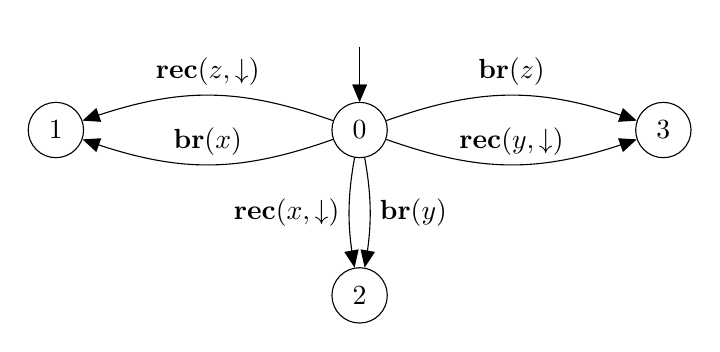
\begin{tikzpicture}[xscale=0.5,AUT style,node distance=2.1cm,auto,>= triangle
	45]
	\tikzstyle{initial}= [initial by arrow,initial text=,initial
	distance=.7cm, initial above]
	%	\tikzstyle{accepting}= [accepting by arrow,accepting text=,accepting
	%	distance=.7cm,accepting where =right]
	
	\node[state,initial, minimum width=0.1pt] (0) at (0,0) {0};
	\node[state] [left of=0, xshift=-50] (x) {1};
	\node[state] [below of=0] (y) {2};
	\node[state] [right of=0, xshift=50] (z) {3};

	\path[->, bend left=10] 	
	(0) edge node[above] {$\brone{x}$} (x)
	(0) edge node {$\brone{z}$} (z)
	;
	\path[->, bend right=10] 	
	(0) edge node[above] {$\recone{y}{\enregact}$} (z)
	(0) edge node[above] {$\recone{z}{\enregact}$} (x)
	;
	\path[->, bend left=20] 	
	(0) edge node {$\brone{y}$} (y)
	;
	\path[->, bend right=20] 	
	(0) edge node[left] {$\recone{x}{\enregact}$} (y)
	;
\end{tikzpicture}
		\caption{An illustrating example}
		\label{fig:no-clique}
	\end{figure}
\end{example}



\begin{definition}
	We say that a "query" $\query$ is ""contradictory"" if either:
	\begin{itemize}
		\item there exists $\varz$ and $q \neq q' \in Q$ such that $\quotemarks{q(\varz)}, \quotemarks{q'(\varz)} \in \query$ or
		
		\item there exist $\var{z_1}, \ldots, \var{z_k} \in \varset$ and $j_1, \ldots, j_k$ with $k\geq 1$ such that $\quotemarks{R_{j_i}(\varz_{i}) = R_{j_{i+1}}(\varz_{i+1})} \in \query$ for all $i \in \set{1,\ldots,k-1}$ and $\quotemarks{R_{j_k}(\varz_k) \neq R_{j_1}(\varz_1)} \in \query$.
	\end{itemize}
\end{definition}

\begin{proposition}
	A "query" $\query$ is "contradictory" if and only if there exists no configuration satisfying $\query$. Additionnaly, one may decide whether $\query$ is contradictory in time polynomial in $\size{\prot} + \size{\query}$. 
\end{proposition}

\ifproofs
\begin{proof}
	Suppose first that $\query$ is "contradictory". If there exist $q \ne q'$ such that
	$\quotemarks{q(\varz)}, \quotemarks{q'(\varz)} \in \query$,  then a "configuration" satisfying $\query$ would need to have a single agent in two distinct states. If there exist $\var{z_1}, \ldots, \var{z_k}$ distinct variables with $k\geq 1$ such that $\quotemarks{R(\varz_{i}) = R(\varz_{i+1})} \in \query$ for all $i \in \set{1,\ldots,k-1}$ and $\quotemarks{R(\varz_k) \neq R(\varz_1)} \in \query$, then in any configuration satisfying $\query$,  the registers associated with $\varz_k$ and $\varz_1$ must have the same register value but also distinct register values, which is a contradiction. 
	
	Suppose now that the $\query$ is not "contradictory" and show that there exists some configuration satisfying $\query$.
	
	We consider the graph $G$ whose vertices are variables of $\varset$ appearing in $\query$ and with an edge between $\varz$ and $\varz'$ if and only if $R(\varz) = R(\varz') \in \query$. Since $\query$ is not "contradictory", for any $\varz, \varz'$ in the same connected component of $G$, $\quotemarks{R(\varz) \ne R(\varz')} \notin \query$. We construct a configuration satisfying $\query$ with an agent $a_\varz$ for every $\varz$ such that:
	\begin{itemize}
		\item if $\quotemarks{q(\varz)} \in \query$ then $a_\varz$ is in state $q$,
		\item the agents of the variables of a connected component of $G$ have all the same register value.  
	\end{itemize}
	The built configuration satisfies $\query$, which concludes the proof. 
\end{proof}
\fi

\begin{lemma}
	\label{lem:query-decomposition}
	Let $\query$ a  "non-contradictory" "query". There exist $K_1, \ldots, K_p \subseteq Q$ with $p \leq \size{\query}$ with the following property: there exists a "run" satisfying $\query$ if and only if for all $i \in \set{1,\ldots, p}$, there is a run satisfying $K_i$. Moreover,such sets $K_1, \dots, K_p$ may be computed in time polynomial in $\size{\prot}$. 
\end{lemma}


\ifproofs
\begin{proof}
	
	We consider the same graph $G$ as in the previous proof. We decompose $G$ into connected components $C_1, \ldots, C_p$. 
	For each $C_i$ we define $K_i = \set{q \in Q \mid \exists \varz \in C_i, q(\varz) \in \query}$. Note that $K_i$ may be empty when there is no constraints on the states of the variables in $C_i$. An empty set is satisfied by any "run". This is coherent with the fact that, when $K_i = \emptyset$, it suffices to assign all variables in $C_i$ to an agent that stays in $q_0$ for the whole "run".
	
	Suppose there is a "run" satisfying $\query$, let $\config$ be its final configuration, let $\nu$ be a valuation witnessing the satisfaction of $\query$ by $\config$.
	Let $i \in \set{1,\ldots, p}$, we show that $\config$ satisfies $K_i$. For all $\varz \in C_i$, let $(q_\varz,\aval_\varz) = \config(\nu(\varz))$. As $C_i$ is a connected component of $G$ and $\config$ satisfies $\query$, all $\nu(\varz)$ with $\varz \in C_i$ have the same register value, which we call $\aval$. 
	For all $q \in K_i$, there exists $\varz \in C_i$ such that $q(\varz) \in \query$ and thus $q_\varz =q$ and $\aval_\varz =\aval$, thus $C_i$ is satisfied.
	
	For the converse implication, suppose for all $i$ we have a run $\run_i$ over a set of agents $\agents_i$ satisfying $K_i$. We rename agents so that the $\agents_i$ are pairwise disjoint, we introduce fresh agents $a_1, \ldots, a_p$ and we set $\agents = \set{a_1, \ldots, a_p} \sqcup \bigsqcup_{i=1}^p \agents_i$. We consider $\run: \config_0 \step{*} \config$ a "run" in which the sequences of actions of each $\run_i$ are executed sequently by agents from $\agents_i$. In $\run$, agents $a_1$ to $a_p$ are left idle on $q_0$. We build the valuation $\nu$ witnessing that $\run$ satisfies $\query$ as follows. Let $i \in \nset{1}{p}$. If $K_i = \emptyset$ then $\nu$ assigns $a_i$ to every variable of $C_i$. Otherwise, we know that $\config|_{\agents_i}$ satisfies $K_i$ because the final configuration of $\run_i$ does: there exists $\aval_i \in \nats$ such that, for all $q \in K_i$, some agent $a_{i,q}$ has state $q$ and register value $\aval_i$ in $\config$. Let $\varz \in C_i$. If, for some $q \in Q$, $\quotemarks{q(\varz)} \in \query$, $\nu$ assigns agent $a_{i,q}$ to $\varz$ ($q$ is unique as $\query$ is not "contradictory"). If $\query$ has no constraint about the state of $\varz$, $\nu$ assigns to $\varz$ some $a_{i,q}$ with $q \in k_i$ arbitrary. 
	
	% We define a valuation $\nu$ as follows. Let $\varz \in \varset$ and $i$ so that $C_i$ is the connected component of $\varz$ in $G$. If  for some $q$, then this $q$ is unique as $\query$ is not "contradictory". We set $\nu(\varz) = a_q^i$.
	% If there is no $q(\varz)$ for any $q \in Q$ in $\query$ but there is one of the form $q'(\varz')$ with $\varz' \in C_i$, then we set $\nu(\varz) = \nu(\varz')$.
	% Otherwise we set $\nu(\varz) = a_i$.
	% This fully defines our valuation $\nu$.
	
	Clearly all formulas of the form $q(\varz)$ or $R(\varz) = R(\varz')$ are satisfied.
	For the formulas of the form $R(\varz) \neq R(\varz')$, we observe that as $\query$ is not "contradictory", $\varz$ and $\varz'$ are not in the same connected component of $G$. Because the runs $\run_i$ worked with disjoint sets of register values ($\config_0$ is initial), the agents assigned to $\varz$ and $\varz'$ end the run with distinct register values.
	Hence $\data{\config}(\nu(\varz)) \neq \data{\config}(\nu(\varz'))$. As a result, $\query$ is satisfied by $\run$.
\end{proof}
\fi
\fi


\subsection{Classical definitions}
\luin{here comes definitions of complexity classes, wqo and anything not related to our model}

\paragraph*{Fast-growing hierarchy}

For $\alpha$ an ordinal in Cantor normal form, we will denote by $\Ffunction{\alpha}$ the class of functions corresponding to level $\alpha$ in the Fast-Growing Hierarchy. We will moreover denote by $\Fcomplexity{\alpha}$ the associated complexity class and use the notion of $\Fcomplexity{\alpha}$-completeness. All these notions are defined in \cite{Schmitz13}. We will specifically work with complexity class $\Fcomplexity{\omega^{\omega}}$. For readers unfamiliar with these notions, $\Fcomplexity{\omega^{\omega}}$-complete problems are problems which are decidable but with very high complexity (they are non-primitive recursive, and even hyper-Ackermannian). 

We highlight that our main result is the decidability of the problem. In fact, proving that the problem lies in $\Fcomplexity{\omega^{\omega}}$ does not complicate our decidability proof significantly. Moreover, this result fits nicely into the landscape of high-complexity problems arising from well quasi-orders. 

\paragraph*{Well-quasi orders}

In order to prove our main decidability result, we rely on the theory of well quasi-orders in the context of the subword ordering.
Let $\Sigma$ be a finite alphabet, $w_1, w_2 \in \Sigma^*$, $w_1$ is a ""subword"" of $w_2$, denoted $w_1 \subword w_2$, when $w_1$ can be obtained from $w_2$ by erasing some letters. 
A sequence of words $w_0, w_1, \ldots$ is ""good"" if there exist $i<j$ such that $w_i \subword w_j$, and ""bad"" otherwise. Higman's lemma \cite{Higman52} states that every "bad" sequence of words over a finite alphabet is finite.
However, this will not suffice us as we will need a bound the length of a "bad" sequence. In order to obtain such a bound, it is necessary to bound the growth of the sequence of words. 
We will use the following result, known as the "Length function theorem" \cite{SchmitzS2011upperHigman}:

\begin{theorem}[Length function theorem \cite{SchmitzS2011upperHigman}]
	\label{lem:lengthfcttheorem}
	Let $\Sigma$ be a finite alphabet, let $g : \nats \to \nats$ be a primitive recursive function, $n\in \nats$.
	Then there exists a function $f \in \Ffunction{\omega^{\size{\Sigma} - 1}}$ such that every "bad sequence" $w_0, w_1, \ldots$ such that $\size{w_i} \leq g^{(i)}(n)$ for all $i$ is of length at most $f(n)$. 
\end{theorem}



\subsection{Link with LCS}

""Lossy channel systems"" ("LCS") are systems where finite-state processes communicate via sending messages from a finite alphabet through unbounded FIFO channels through which messages may be lost. The reachability problem asks whether a given control state of the system may be covered. Unlike in the non-lossy case \cite{BZ83}, reachability is decidable for "lossy channel systems" \cite{AK95,AbdullaJ1996undec}, but is proven to have non-primitive recursive complexity \cite{Schnoebelen2002verifying} and is in fact $\Fcomplexity{\omega^{\omega}}$-complete \cite{ChambartS2008ordinal}.

We argue that the "coverability problem" in BNRA is at least as hard as the reachability problem for "LCS", even with two registers. The reduction can be found in Appendix~\ref{app:reduction-lcs}; we provide here some intuition. Given a LCS $\los$, we build a protocol $\prot$ with two registers. In this protocol, register $1$ plays the role of the identifier and is read-only. Agents use their second register to store another agent's identifier at the start; an agent only accepts messages with this identifier, using an $\quotemarks{\eqtestact}$ on every reception. This way, agents will form chains where messages propagate in one direction only, with the property that an agent has at most one predecessor in the chain. Each agent of the chain will simulate a step of an execution of $\los$: an agent received from its predecessor a configuration of $\los$, chooses the next configuration of $\los$ and broadcasts it, sending first the location of $\los$ then, letter by letter, the content of the channel. Note that some letters of the channel might not be received, hence the lossiness. 
% Note that one special agent has to start the execution, and send the initial configuration before receiving anything. The final state is the final state of the "LCS" and if one agent reaches it, one can argue that there is an execution of the "LCS" described by the sent messages in the chain of agent starting with an agent sending the initial configuration.

\begin{restatable}{proposition}{propReductionLCS}
	\label{prop:reduction-LCS}
	The "coverability problem" for BNRAs is $\Fcomplexity{\omega^\omega}$-hard.
\end{restatable}

%The proof is in Appendix~\ref{app:reduction-lcs}.

\begin{remark}
	The reduction presented in the proof of Proposition~\ref{prop:reduction-LCS} can be adapted to show that the repeat coverability problem is undecidable for BNRA, as it is for LCS.
\end{remark}


	\section{Coverability Decidability for Signature Protocols}
\label{sec:cover-decidability}

This section and the next one are dedicated to the proof of our main result:

\begin{restatable}{theorem}{decidablecover}
\label{thm:decidable-cover}
\COVER for BNRA is decidable and $\Fcomplexity{\omega^\omega}$-complete.
\end{restatable}

For the sake of clarity, in this section, we will first focus on the case of "signature BNRA". 
As a preliminary, we start by defining a notion of "local run" meant to represent the projection of a run onto a given agent.

\subsection{Local runs}
\AP A ""local configuration"" is a pair $(q, \localdata) \in Q \times \nats^r$.  
\AP An ""internal step"" from $(q,\localdata)$ to $(q',\localdata')$ with transition $\atrans \in \transitions$, denoted $(q,\localdata) \intstep{\atrans} (q',\localdata')$, is defined when $\localdata = \localdata'$ and $\atrans =(q, \br{m}{i}, q')$ is a "broadcast".  
\AP A ""reception step"" from $(q,\localdata)$ to $(q',\localdata')$ with transition $\atrans \in \transitions$ and value $\aval \in \nats$, denoted $(q,\localdata) \extbr{\atrans}{\aval} (q',\localdata')$, is defined when $\atrans$ is of the form $(q,\rec{m}{j}{\anact},q')$ with $\localdata(j') = \localdata'(j')$ for all $j' \neq j$ and:
	
	\begin{minipage}[t]{6cm}
		\begin{itemize}
			\item if $\anact = \quotemarks{\dummyact}$ 
			then $\localdata(j) = \localdata'(j)$,
			\item if $\anact = \quotemarks{\enregact}$ then $\localdata'(j) = v$,
		\end{itemize}
	\end{minipage}
	\begin{minipage}[t]{6cm}
		\begin{itemize}
			\item if $\anact = \quotemarks{\eqtestact}$ then $\localdata(j) = \localdata'(j)= v$,
			\item if $\anact = \quotemarks{\diseqtestact}$ then $\localdata(j) = \localdata'(j) \ne v$.
		\end{itemize}
	\end{minipage}
	

	%Said otherwise, $(q,\localdata) \extbr{\atrans}{\aval} (q',\localdata')$ when an agent in $(q,\localdata)$ may perform $\atrans$ upon receiving a message of type $\amessage$ and of value $\aval$.
	\AP A ""local step"" $(q,\localdata) \step{} (q',\localdata')$ is either a "reception step" or an "internal step". 
	\AP A ""local run"" $\localrun$ is a sequence of "local steps" denoted $(q_0, \nu_0) \step{*} (q, \nu)$. Its ""size@@localrun"" $\size{\localrun}$ is its number of steps. %where $\nu_0$ has distinct values.
	A value $\aval \in \nats$ appearing in $\localrun$ is ""initial"" if it appears in $\nu_0$ and ""non-initial"" otherwise. 
%	The ""input"" of $\localrun$, written $\intro*\Input{\localrun} \in (\messages \times \nats)^*$, is the sequence of messages received in $\localrun$; its ""output"", written $\intro*\Output{\localrun} \in (\messages \times \nats)^*$, is the sequence of messages broadcast in $\localrun$. 
	% The $\aval$-input $\vinput{\aval}{\localrun}$ (resp. $\val$-output $\voutput{\aval}{\localrun}$) is the sequence containing message types of "reception steps" (resp. broadcast steps) of $\localrun$ with value $\val$. 
	For $\aval \in \nats$, the $\aval$-""input"" $\intro*\vinput{\aval}{\localrun}$ (resp. $\aval$-""output"" $\intro*\voutput{\aval}{\localrun}$) is the sequence $m_0 \cdots m_{\ell} \in \messages^*$ of message types received (resp. broadcast) with value $\aval$ in $\localrun$.

\subsection{Unfolding Trees}
\label{sec:unfolding_tree_signature}

We first prove decidability of \COVER for "signature BNRA". Note that, in "signature protocols", the initial values of "reception-only" registers are not relevant as they can never be shared with other agents. We deduce from this idea the following informal observation:
\begin{observation}
\label{obs:sg_reception} 
In "signature BNRA", when some agent receives a message, it can compare the value of the message only with the ones of previously received messages, \emph{i.e.}, check whether the sender is the same.
\end{observation}

If we want to turn a "local run" $u$ of an agent $a$ into an actual "run", we must match $a$'s receptions with broadcasts. Because of Observation~\ref{obs:sg_reception}, what matters is not the actual values of the receptions in $u$ but which ones are equal to which.  Therefore, for a value $v$ received in $u$, if $m_1 \dots m_k \in \messages^*$ are the message types received in $u$ with value $v$ in this order, it means that to execute $u$, $a$ need another agent $a'$ to broadcast messages types $m_1$ to $m_k$, all with the same value.  
We describe what an agent needs from other agents as a set of ""specifications@@sg"" which are words of $\messages^*$. 
% A ""specification@@sg"" $m_1 \cdots m_k \in \messages^*$ is accomplished by an agent if it broadcasts message types $m_1, \dots, m_k$ in this order. 

To represent runs, we consider "unfolding trees@@signature" that abstract runs by representing such specifications, dependencies between them and how they are carried out. In this tree, each node is assigned a "local run" and the "specification@@sg" that it carries out. 
Because of copycat arguments, we will in fact be able to duplicate agents so that each agent only accomplishes one task, hence the tree structure.

\begin{definition}
\label{def:unfolding_tree_signature}
\AP An ""unfolding tree@@sg"" $\tree$ over $\prot$ is
a finite tree where nodes $\node$ have three labels:
\begin{itemize}
	\item a "local run" of $\prot$, written $\intro*\localrunlabel{\node}$;
	
	\item a value in $\nats$, written $\intro*\valuelabel{\node}$;
	
	\item a "specification" $\intro*\speclabel{\node} \in \messages^*$.
\end{itemize} 
Moreover, all nodes $\node$ in $\tree$ must satisfy the three following conditions:
\begin{enumerate}[label= (\roman*), ref=(\roman*)]
	\item \label{item:condition1_initial_value_sg} Initial values of $\localrunlabel{\node}$ are never received in $\localrunlabel{\node}$,
	\item \label{item:condition3_boss_node_sg} $\speclabel{\node} \subword \voutput{\valuelabel{\node}}{\localrunlabel{\node}}$, \emph{(recall that $\subword$ denotes the "subword" relation)}
	\item \label{item:condition2_non_initial_value_sg} For each value $\aval$ received in $\localrunlabel{\node}$, $\node$ has a child $\node'$ s.t. $\vinput{\aval}{\localrunlabel{\node}} \subword \speclabel{\node'}$.
\end{enumerate}

\AP Lastly, given $\tree$ an "unfolding tree@@sg", we define its ""size@@treesg"" by $\size{\tree} := \sum_{\node \in \tree} \size{\node}$ where $\size{\node} := \size{\localrunlabel{\node}} + \size{\speclabel{\node}}$. Note that the "size@@treesg" of $\tree$ takes into account the size of its nodes, so that a tree $\tree$ can be stored in space polynomial in $\size{\tree}$ (renaming the values appearing in $\tree$ if needed). 
\end{definition}
% subword explaination

We explain this definition. Condition \ref{item:condition1_initial_value_sg} enforces that the "local run" cannot cheat by receiving its "initial values". 
 Condition \ref{item:condition3_boss_node_sg} expresses that $\localrunlabel{\node}$ broadcasts (at least) the messages of $\speclabel{\node}$. We can use the subword relation $\subword$, and not equality, because of the lossiness: if some unecessary messages are broadcast, simply consider that they are not received.
Condition \ref{item:condition2_non_initial_value_sg} expresses that, for each value received, $\node$ has a child that broadcasts the right sequence of messages.

\begin{figure}[t]
	\centering
	\resizebox*{!}{3.5cm}{
	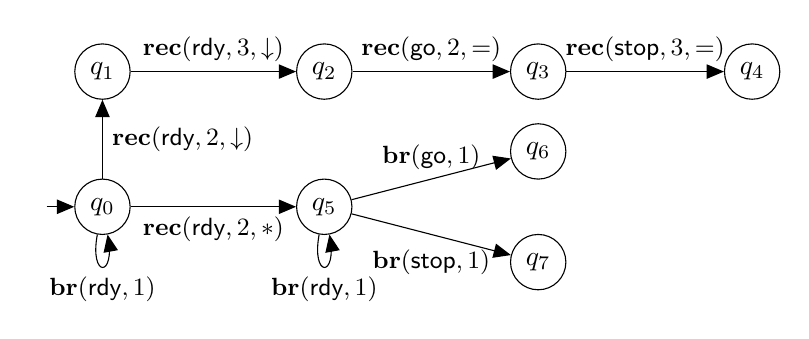
\begin{tikzpicture}[xscale=0.5,AUT style,node distance = 2cm,auto,>= triangle 45]
	\tikzstyle{initial}= [initial by arrow,initial text=,initial
	distance=.7cm]
	%	\tikzstyle{accepting}= [accepting by arrow,accepting text=,accepting
	%	distance=.7cm,accepting where =right]
	

	% \node[state,initial] {$q_0$};
	\node[state, initial] (0) {$q_0$};
	\node[state] [above = 1 of 0] (1) {$q_1$};
	\node[state] [right = 2.1 of 1] (2) {$q_2$};
	\node[state] [right = 2 of 2] (3) {$q_3$};
	\node[state] [right = 2 of 3] (4) {$q_4$};
	\node[state] [right = 2.1 of 0] (5) {$q_5$};
	\node[state] [right = 2 of 5, yshift = 20] (6) {$q_6$};
	\node[state] [right = 2 of 5, yshift = -20] (7) {$q_7$};
	
%	\node[state] [right = 2.5 of 4] (5) {$q_5$};
	
	
	%	\path[->, bend left=10] 	
	%	(0) edge node[above, xshift=-10] {$\br{init}{1}$} (x)
	%	;
	%	\path[->, bend right=10] 	
	%	(0) edge node[below, xshift=-10] {$\rec{init}{2}{\enregact}$} (y)
	%	;
	\path[->] 	
%	(0)  edge [out=240,in=300,looseness=3] node[below, xshift = -20] {\small$\br{\exready}{1}$} (0)
			
	(5) edge node[above] {\small$\br{\exgotwo}{1}$} (6)
	(5) edge node[below, yshift = -2] {\small$\br{\exgothree}{1}$} (7)
	(5) edge [out = -105, in = -75, looseness = 4] node[below] {\small$\br{\exready}{1}$} (5)
	(0) edge [out = -105, in = -75, looseness = 4] node[below] {\small $\br{\exready}{1}$} (0)
	(0) edge node[right] {\small $\rec{\exready}{2}{\enregact}$} (1)
	(1) edge node {\small $\rec{\exready}{3}{\enregact}$} (2)
	(2) edge node {\small $\rec{\exgotwo}{2}{\eqtestact}$} (3)
	(3) edge node {\small $\rec{\exgothree}{3}{\eqtestact}$} (4)
	(0) edge node [below]{\small $\rec{\exready}{2}{\dummyact}$} (5)


	;
	
\end{tikzpicture}
	}
	\caption{Example of a "signature protocol".}\label{fig:ex2}\label{fig:example-signature-protocol}
\end{figure}
\begin{example}
\label{ex:protocol-signature}
	Figure~\ref{fig:example-signature-protocol} provides an example of a "signature protocol".
Let $\agents = \set{a_1, a_2,a_3}$. We denote a configuration $\config$ by $\tuple{\st{\config}(a_1),(\data{\config}(a_1)), \\ \st{\config}(a_2),(\data{\config}(a_2)), \st{\config}(a_3), (\data{\config}(a_3))}$. Irrelevant register values are denoted by $\_$. Let $\run$ be the run over $\agents$ of initial configuration  \\$\tuple{q_0, (1,\_,\_), q_0, (2,\_,\_), q_0, (3,\_,\_)}$ where the following occurs:
\begin{itemize}
\item $a_2$ broadcasts $\exready$, $a_1$ receives: $\tuple{q_1, (1,2,\_), q_0, (2,\_,\_), q_0, (3,\_,\_)}$,
\item $a_3$ broadcasts $\exready$, $a_1$ and $a_2$ receive: $\tuple{q_2, (1,2,3), q_5, (2,\_,\_), q_0, (3,\_,\_)}$,
\item $a_2$ broadcasts $\exready$, $a_3$ receives: $\tuple{q_2, (1,2,3), q_5, (2,\_,\_), q_5, (3,\_,\_)}$,
\item $a_2$ broadcasts $\exgotwo$, $a_1$ receives: $\tuple{q_3, (1,2,3), q_6, (2,\_,\_), q_5, (3,\_,\_)}$,
\item $a_3$ broadcasts $\exgothree$, $a_1$ receives: $\tuple{q_4, (1,2,3), q_6, (2,\_,\_), q_7, (3,\_,\_)}$.
\end{itemize}
	
Figure~\ref{fig:ex-unfolding-tree-signature} provides an unfolding tree derived from $\run$ by applying a procedure introduced later. Because agents $a_2$ and $a_3$ broadcast to several other agents, they each correspond to several nodes of the tree.  
% the following sequence is an initial run covering $q_4$:
	% \begin{align*}
	% 	&\tuple{(q_0, (\valsymb{1},2,3)), (q_0, (x_2,\_,\_)) , (q_0, (x_3,\_,\_))} \step{} \tuple{(q_1, (x_1,x_2,z_1)), (q_5,(x_2,\_,\_)) , (q_0, (x_3,\_,\_))} \step{} \\ 
	% 	&\tuple{(q_2, (x_1,x_2,x_3)), (q_5,(x_2,\_,\_)), (q_5, (x_3,\_,\_))} \step{} \tuple{(q_3, (x_1,x_2,x_2)), (q_5,(x_2,\_,\_)), (q_5, (x_3,\_,\_))} \step{} \\
	% 	&\tuple{(q_4, (x_1,x_2,x_2)),(q_5,(x_2,\_,\_)), (q_5, (x_3,\_,\_))} 
	% \end{align*}
	% For readability's sake we don't write the second and third registers' values of agent $a_2$ and $a_3$ as there are neither broadcast, tested and nothing is store on those registers during the run.
	% First agent $a_2$ broadcasts message $hello$ with its second register's value, then $a_3$ broadcasts message $hey$ with its third register's value. Then, agent $a_2$ broadcasts message $ack$ with its second register's value and finally, agent $a_3$ broadcasts the same message but with its third register's value.
	% All messages are received by agent $a_1$ which hence reaches $q_4$.
	% We show now how to build the unfolding tree regarding the local run of agent $a_1$ in \cref{fig:unfolding-tree-sign}. Tables are (part of) "local runs", columns are (part of) "local configurations": we only display registers used in the local runs (the one broadcast or with a reception action on it). For $\node_2$, the transition between $q_0$ and $q_5$ should be understood as the broadcast of $hello$, whereas for $\node_3$ it should be understand as the broadcast of $hey$.
	% The local run of node $\node_1$ is the local run of agent $a_1$ of the run described above. 
	% By completing partial local runs by fresh integers in the other registers, one can verify that all nodes are labeled by local runs of the protocol (where the broadcast between $q_0$ and $q_5$ is with $hello$ for $\node_2$, and with $hey$ for $\node_3$).

	We explain why this tree is an "unfolding tree@@sg". Condition \ref{item:condition1_initial_value_sg} is trivially satisfied. 
	Condition \ref{item:condition3_boss_node_sg} holds at every node because the local run of each node exactly broadcasts the "specification@@sg" of the node. Condition  \ref{item:condition2_non_initial_value_sg} is satisfied at $\node_1$: $\vinput{2}{\localrunlabel{\node_1}}= \exready \cdot \exgotwo = \speclabel{\node_2}$ and $\vinput{3}{\localrunlabel{\node_1}}= \exready \cdot \exgothree = \speclabel{\node_3}$.
	It is also satisfied at $\node_2$, $\node_3$ and $\node_5$ because their local runs only receive $\exready$ and they each have a child with "specification@@sg" $\exready$. 
	It is trivially satisfied at $\node_4$ and $\node_6$ as their "local runs" have no reception. 
%	\corto{shorten?} \nico{plutôt non je dirais}
	% Values received in $\localrunlabel{\node_1}$ are $x_2$ and $x_3$, hence from condition \ref{item:condition2_non_initial_value_sg}, node $\node_1$ has two children $\node_2$ and $\node_3$. Note that $\vinput{x_2}{\localrunlabel{\node_2}} = \vinput{x_3}{\localrunlabel{\node_3}} = \epsilon$\lu{si on modifie la condition, on peut enlever cette phrase}. As $\spec(\node_1) = \epsilon$, condition \ref{item:condition3_boss_node_sg} is trivially true for $\node_1$. Note that nodes $\node_2$ and $\node_3$ don't receive any message on their respective local runs and so condition \ref{item:condition2_non_initial_value_sg} is trivially true. Furthermore, $\voutput{x_2}{\localrunlabel{\node_2}} = hello \cdot ack = \spec(\node_2)$ and $\voutput{x_3}{\localrunlabel{\node_3}} = hey \cdot ack = \spec(\node_3)$
\end{example}


\begin{figure}[t]
	\centering
	\newcommand{\tikzabstractconfig}[5]{% x, y, val1, val2, q, x1, y1
	\begin{tikzpicture}
		\draw (#1,#2) rectangle (1 + #1,0.5 +#2);
		\draw (#1,-0.5 + #2) rectangle (1 +#1 ,#2);
		\node[] (x1) at (0.5 + #1, 0.15 +#2) {#3};
		\node[] (x2) at (0.5 +#1 , 0.15- 0.5 +#2) {#4};
		\node [] (q) at (0.5 +#1, 0.7+#2) {#5};
	\end{tikzpicture}
}

\newcommand{\tikzvalue}[4]{% x, y, length, val
	\begin{tikzpicture}
		\node [] (v) at (#1 + #3 + 0.3, #2 + 1.2) {$\mathbf{v}= #4$};
	\end{tikzpicture}
}

\newcommand{\tikzspec}[4]{% x, y, length, spec
	\begin{tikzpicture}
		\node [] (sp) at (#3 /2, #2 - 0.2) {#4};
	\end{tikzpicture}
}

\newcommand{\displayone}[1]{{\color{Yellow!70!black} #1}}
\newcommand{\displaytwo}[1]{{\color{cyan} #1}}
\newcommand{\displaythree}[1]{{\color{Red} #1}}
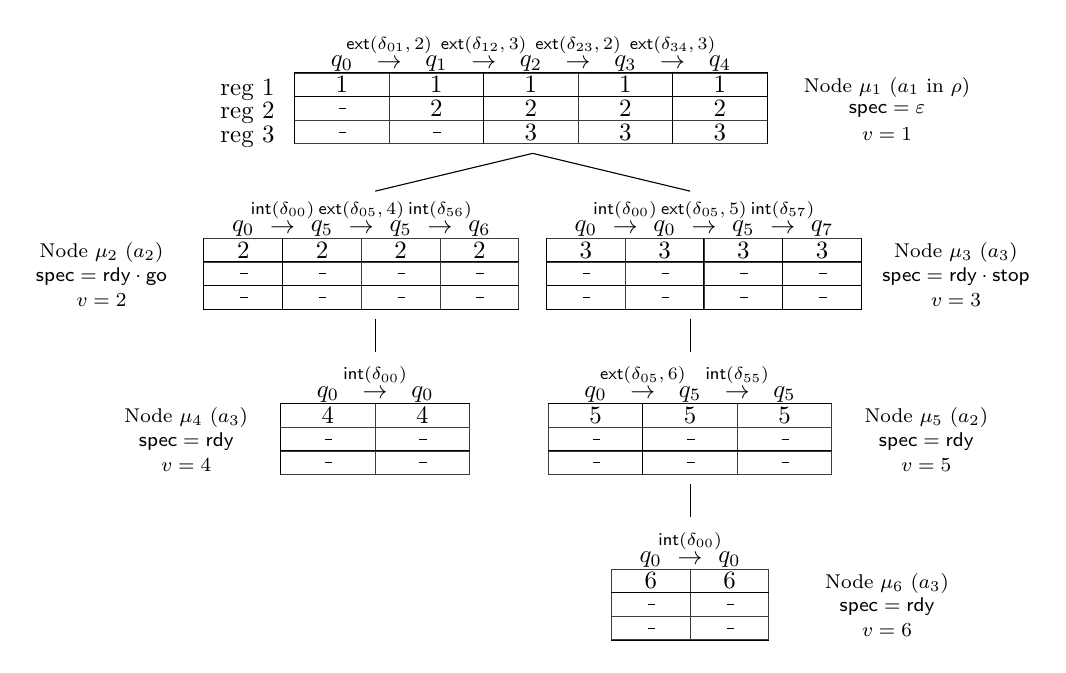
\begin{tikzpicture} [xscale = 1, yscale = 0.6, every node/.style = {scale = 0.9}]
	
	%	
	%	\tikzabstractconfig{0}{0}{$x_1$}{$y_1$}{$q_0$}
	%	\tikzabstractconfig{1}{0}{$x_1$}{$y_1$}{$q_1$}
	%	\tikzabstractconfig{2}{0}{$x_1$}{$y_2$}{$q_4$}
	%	\tikzabstractconfig{3}{0}{$x_1$}{$y_2$}{$q_6$}
	% \node [] (sp) at (6, 0.2) {Node $\node_1$};
	% \node [] (sp) at (6, 0.2-0.5) {$\spec(\node_1) = \epsilon$};
	% \node [] (sp) at (6, 0.2-1) {$v = 1$};
	% \draw (-0.5,0) rectangle (0.5,0.5);
	% \draw (-0.5,-0.5 ) rectangle (0.5 ,0);
	% \draw (-0.5,-0.5) rectangle (0.5,-1);
	% \node (reg1) at (-1, 0.15) {reg $1$};
	% \node (reg2) at (-1, 0.15-0.5) {reg $2$};
	% \node (reg3) at (-1, 0.15-0.5-0.5) {reg $3$};

	% \node[] (x1) at (0, 0.15) {$1$};
	% \node[] (x2) at (0 , 0.15- 0.5) {$\_$};
	
	% \node[] (x2) at (0 , 0.15- 0.5-0.5) {$\_$};
	% \node [] (q) at (0 , 0.7) {$\_$};
	
	% \draw (0.5,0) rectangle (1.5,0.5);
	% \draw[fill = orange, opacity=0.4]  (0.5,-0.5) rectangle (1.5,0);
	% \draw (0.5,-0.5 ) rectangle (1.5 ,0);
	% \draw (0.5,-1) rectangle (1.5,-0.5);
	% \node[] (x1) at (1, 0.15) {$1$};
	% \node[] (x2) at (1 , 0.15- 0.5) {$2$};
	% \node[] (x2) at (1 , 0.15- 0.5-0.5) {$\_$};
	% \node [] (q) at (1 , 0.7) {$q_1$};
	
	% \draw (1.5,0) rectangle (2.5,0.5);
	% \draw[fill = orange, opacity=0.4] (1.5,-0.5) rectangle (2.5,0.5-0
	% .5);
	% \draw (1.5,-0.5 ) rectangle (2.5 ,0);
	% \draw[fill = white, opacity=0.4] (1.5,-0.5-0
	% .5 ) rectangle (2.5 ,0-0
	% .5);
	% \draw (1.5,-0.5-0.5 ) rectangle (2.5 ,0-0.5);
	% \node[] (x1) at (2, 0.15) {$1$};
	% \node[] (x2) at (2 , 0.15- 0.5) {$2$};
	% \node[] (x2) at (2 , 0.15- 0.5-0.5) {$3$};
	% \node [] (q) at (2 , 0.7) {$q_2$};
	
	
	% \draw[] (2.5,0) rectangle (3.5,0.5);
	% \draw[fill = orange, opacity=0.4] (2.5,0-0.5) rectangle (3.5,0.5-0.5);
	% \draw (2.5,-0.5 ) rectangle (3.5 ,0);
	% \draw[fill = white, opacity=0.4]  (2.5,-0.5-0.5 ) rectangle (3.5 ,0-0.5);
	% \draw (2.5,-0.5 -0.5) rectangle (3.5 ,0-0.5);
	% \node[] (x1) at (3, 0.15) {$1$};
	% \node[] (x2) at (3 , 0.15- 0.5) {$2$};
	% \node[] (x2) at (3 , 0.15- 0.5-0.5) {$3$};
	% \node [] (q) at (3 , 0.7) {$q_3$};
	
	% \draw[] (3.5,0) rectangle (4.5,0.5);
	% \draw[fill = orange, opacity=0.4] (3.5,0-0.5) rectangle (4.5,0.5-0.5);
	% \draw (3.5,-0.5 ) rectangle (4.5 ,0);
	% \draw[fill = white, opacity=0.4]  (3.5,-0.5 -0.5) rectangle (4.5 ,0-0.5);
	% \draw (3.5,-0.5-0.5 ) rectangle (4.5 ,0-0.5);
	% \node[] (x1) at (4, 0.15) {$1$};
	% \node[] (x2) at (4 , 0.15- 0.5) {$2$};
	% \node[] (x2) at (4 , 0.15- 0.5-0.5) {$3$};
	% \node [] (q) at (4 , 0.7) {$q_4$};
	

	\node [font = {\footnotesize}] (sp) at (6.5, 0.2-0.5) {Node $\node_1$ ($a_1$ in $\run$)};
	\node [font = {\footnotesize}] (sp) at (6.5, 0.2-1) {$\spec = \epsilon$};
	\node [font = {\footnotesize}] (sp) at (6.5, 0.2-1.5) {$v = 1$};
	\begin{scope}[xscale = 1.2, xshift = -10]
	\regbar{-1}{0}
	\onerow{-0.5}{0}{$q_0$}{$1$}{white}{$\_$}{white}{$\_$}{white}
	\transtable{0.5}{0}{$\displayone{\extlabel{\atrans_{01}}{2}}$}
	% \node [align = center] at (0.5, 0.2) {$\rightarrow$};
	% \node [align = center, font = {\tiny}] at (0.5,0.5) {$\extlabel{\atrans_{01}}{2}$};
	\onerow{0.5}{0}{$q_1$}{$1$}{white}{$2$}{white}{$\_$}{white}
	\transtable{1.5}{0}{$\displayone{\extlabel{\atrans_{12}}{3}}$}
	\onerow{1.5}{0}{$q_2$}{$1$}{white}{$2$}{white}{$3$}{white}
	\transtable{2.5}{0}{$\displaytwo{\extlabel{\atrans_{23}}{2}}$}
	\onerow{2.5}{0}{$q_3$}{$1$}{white}{$2$}{white}{$3$}{white}
	\transtable{3.5}{0}{$\displaythree{\extlabel{\atrans_{34}}{3}}$}
	\onerow{3.5}{0}{$q_4$}{$1$}{white}{$2$}{white}{$3$}{white}
	\end{scope}
	\draw (2, -1.7) -- (0, -2.5);
	\draw (2, -1.7) -- (4, -2.5);
	
	\begin{scope}[xshift = -5]
	% \regbar{-3.5}{-3}
	\onerow{-2}{-3.5}{$q_0$}{$2$}{white}{$\_$}{white}{$\_$}{white}
	\transtable{-1}{-3.5}{$\displayone{\intlabel{\atrans_{00}}}$}
	\onerow{-1}{-3.5}{$q_5$}{$2$}{white}{$\_$}{white}{$\_$}{white}
	\transtable{0}{-3.5}{$\displayone{\extlabel{\atrans_{05}}{4}}$}
	\onerow{-0}{-3.5}{$q_5$}{$2$}{white}{$\_$}{white}{$\_$}{white}
	\transtable{1}{-3.5}{\displaytwo{$\intlabel{\atrans_{56}}$}}
	\onerow{1}{-3.5}{$q_6$}{$2$}{white}{$\_$}{white}{$\_$}{white}
	\node [align=center, font = {\footnotesize}] (sp) at (-3.3, -3-0.8) {Node $\node_2$ ($a_2$)};
	\node [align = center, font = {\footnotesize}] (sp) at (-3.3,-3.5-0.8) {$\spec = \displayone{\exready} \cdot \displaytwo{\exgotwo}$};
	\node [align = center, font = {\footnotesize}] (sp) at (-3.3, -4-0.8) {$v = 2$};
	\end{scope}
	\begin{scope}[xshift = 5]
	% \regbar{3}{-3}
	\onerow{2}{-3.5}{$q_0$}{$3$}{white}{$\_$}{white}{$\_$}{white}
	\transtable{3}{-3.5}{\displayone{$\intlabel{\atrans_{00}}$}}
	\onerow{3}{-3.5}{$q_0$}{$3$}{white}{$\_$}{white}{$\_$}{white}
	\transtable{4}{-3.5}{$\displayone{\extlabel{\atrans_{05}}{5}}$}
	\onerow{4}{-3.5}{$q_5$}{$3$}{white}{$\_$}{white}{$\_$}{white}
	\transtable{5}{-3.5}{\displaythree{$\intlabel{\atrans_{57}}$}}
	\onerow{5}{-3.5}{$q_7$}{$3$}{white}{$\_$}{white}{$\_$}{white}
	\node [align=center, font = {\footnotesize}] (sp) at (7.2, -3-0.8) {Node $\node_3$ ($a_3$)};
	\node [align = center, font = {\footnotesize}] (sp) at (7.2,-3.5-0.8) {$\spec = \displayone{\exready} \cdot \displaythree{\exgothree}$};
	\node [align = center, font = {\footnotesize}] (sp) at (7.2, -4-0.8) {$v = 3$};
	\end{scope}
\draw (0, -3.5-1.7) -- (0, -3.5-1.7-0.7);
\draw (4, -3.5-1.7) -- (4, -3.5-1.7-0.7);
\begin{scope}[xscale = 1.2, xshift = 0]
	% \regbar{-2.5}{-6}
	\onerow{-1}{-7}{$q_0$}{$4$}{white}{$\_$}{white}{$\_$}{white}
	\transtable{0}{-7}{\displayone{$\intlabel{\atrans_{00}}{}$}}
	\onerow{-0}{-7}{$q_0$}{$4$}{white}{$\_$}{white}{$\_$}{white}
	\node [align=center, font = {\footnotesize}] (sp) at (-2, -3.5-0.8-3) {Node $\node_4$ ($a_3$)};
	\node [align = center, font = {\footnotesize}] (sp) at (-2,-4-0.8-3) {$\spec = {\displayone{\exready}}$};
	\node [align = center, font = {\footnotesize}] (sp) at (-2, -4.5-0.8-3) {$v = 4$};
	\end{scope}
	\begin{scope}[xscale = 1.2, xshift = -19]
	% \regbar{3}{-6}
	\onerow{2.5}{-7}{$q_0$}{$5$}{white}{$\_$}{white}{$\_$}{white}
	\transtable{3.5}{-7}{$\displayone{\extlabel{\atrans_{05}}{6}}$}
	\onerow{3.5}{-7}{$q_5$}{$5$}{white}{$\_$}{white}{$\_$}{white}
	\transtable{4.5}{-7}{\displayone{$\intlabel{\atrans_{55}}$}}
	\onerow{4.5}{-7}{$q_5$}{$5$}{white}{$\_$}{white}{$\_$}{white}
	\node [align=center, font = {\footnotesize}] (sp) at (6.5, -3.5-0.8-3) {Node $\node_5$ ($a_2$)};
	\node [align = center, font = {\footnotesize}] (sp) at (6.5,-4-0.8-3) {$\spec = {\displayone{\exready}}$};
	\node [align = center, font = {\footnotesize}] (sp) at (6.5, -4.5-0.8-3) {$v = 5$};
\end{scope}
\draw (4, -7-1.7) -- (4, -7-1.7-0.7);

	% \regbar{3.5}{-9}
	\onerow{3}{-10.5}{$q_0$}{$6$}{white}{$\_$}{white}{$\_$}{white}
	\transtable{4}{-10.5}{\displayone{$\intlabel{\atrans_{00}}$}}
	\onerow{4}{-10.5}{$q_0$}{$6$}{white}{$\_$}{white}{$\_$}{white}
	\node [align=center, font = {\footnotesize}] (sp) at (6.5, -10-0.8) {Node $\node_6$ ($a_3$)};
	\node [align = center, font = {\footnotesize}] (sp) at (6.5,-10.5-0.8) {$\spec = {\displayone{\exready}}$};
	\node [align = center, font = {\footnotesize}] (sp) at (6.5, -11-0.8) {$v = 6$};

% 	\draw (-2,-3) rectangle (-1,-2.5);
% 	\draw [fill = orange, opacity=0.4] (-2,-2.5) rectangle (-1,-2);
% %	\draw  [fill = white, opacity=0.4] (-2,-3 ) rectangle (-1 ,-2.5);    
% %	\draw  (-2,-3 ) rectangle (-1 ,-2.5);
% 	\node[] (x1) at (-1.5, 0.2 - 2.5) {$x_2$};
% %	\node[] (x2) at (-1.5 , 0.15- 0.5 - 2.5) {$y_2$};
% 	\node [] (q) at (-1.5 , 0.7 - 2.5) {$q_0$};
	
% 	\draw (-1,-2.5) rectangle (0,-2);
% 	\draw [fill = orange, opacity=0.4] (-1,-2.5) rectangle (0,-2);
% %	\draw [fill = white, opacity=0.4] (-1,-3 ) rectangle (0 ,-2.5);    
% %	\draw (-1,-3 ) rectangle (0 ,-2.5);
% 	\node[] (x1) at (-0.5, 0.2 -2.5) {$x_2$};
% %	\node[] (x2) at (-0.5 , 0.15- 0.5 - 2.5) {$y_2$};
% 	\node [] (q) at (-0.5 , 0.7-2.5) {$q_5$};
	
% 	\draw [fill = orange, opacity=0.4] (0,-2.5) rectangle (1,-2);
% 	\draw (0,-2.5) rectangle (1,-2);
% %	\draw (0,-3 ) rectangle (1 ,-2.5);
% %	\draw[fill = white, opacity=0.4] (0,-3 ) rectangle (1 ,-2.5);
% 	\node[] (x1) at (0.5, 0.2 -2.5) {$x_2$};
% %	\node[] (x2) at (0.5 , 0.15- 0.5 - 2.5) {$y_2$};
% 	\node [] (q) at (0.5 , 0.7-2.5) {$q_5$};
	
	
	
	

	

% 	%	\draw (-3,-2) rectangle (-2,0.5 -2);
% 	%	\draw (-3,-0.5 -2) rectangle (1 -3 ,-2);
% 	%\node[] (x1) at (0.5 + #1, 0.15 +#2) {#3};
% 	%\node[] (x2) at (0.5 +#1 , 0.15- 0.5 +#2
% 	%	
% 	%	\tikzabstractconfig{-3}{-2}{$x_1$}{$y_1$}{$q_0$} 
% 	%	\tikzabstractconfig{-2}{-2}{$x_1$}{$y_1$}{$q_1$}
	
	
% 	\draw (3.5,-2.5) rectangle (4.5,-2);
% %	\draw (3.5,-3 ) rectangle (4.5 ,-2.5);
% 	\node[] (x1) at (4, 0.15 - 2.5) {$x_3$};
% %	\node[] (x2) at (4 , 0.15- 0.5 - 2.5) {$y_4$};
% 	\node [] (q) at (4 , 0.7 - 2.5) {$q_0$};
	
% 	\draw (4.5,-2.5) rectangle (5.5,-2);
% 	\draw[fill = white, opacity=0.4]  (4.5,-2.5) rectangle (5.5,-2);
% %	\draw (4.5,-3 ) rectangle (5.5 ,-2.5);
% 	\node[] (x1) at (5, 0.15 - 2.5) {$x_3$};
% %	\node[] (x2) at (5 , 0.15- 0.5 - 2.5) {$y_4$};
% 	\node [] (q) at (5 , 0.7 - 2.5) {$q_5$};
	
% 	\draw (5.5,-2.5) rectangle (6.5,-2);
% 	\draw[fill = white, opacity=0.4] (5.5,-2.5) rectangle (6.5,-2);
% %	\draw (5.5,-3 ) rectangle (6.5 ,-2.5);
% 	\node[] (x1) at (6, 0.15 - 2.5) {$x_3$};
% %	\node[] (x2) at (6 , 0.15- 0.5 - 2.5) {$y_4$};
% 	\node [] (q) at (6 , 0.7 - 2.5) {$q_5$};
	
% %	\draw[fill = white, opacity=0.4] (6.5,-2.5) rectangle (7.5,-2);
% %	\draw (6.5,-2.5) rectangle (7.5,-2);
% %%	\draw (6.5,-3 ) rectangle (7.5 ,-2.5);
% %	\node[] (x1) at (7, 0.15 -2.5) {$x_1$};
% %%	\node[] (x2) at (7 , 0.15- 0.5 - 2.5) {$y_4$};
% %	\node [] (q) at (7 , 0.7-2.5) {$q_4$};
	
% 	\node [] (sp) at (7.6, -2) {Node $\node_3$};
% 	\node [] (sp) at (7.9, -2.5) {$\spec = hey \cdot ack$};
% 	\node [] (sp) at (7.6, -3) {$v = x_3$};
	
	%	\draw (7.5,-2.5) rectangle (8.5,-2);
	%	\draw (7.5,-3 ) rectangle (8.5,-2.5);
	%	\node[] (x1) at (8, 0.2 -2.5) {$x'_2$};
	%	\node[] (x2) at (8 , 0.15- 0.5 - 2.5) {$y_2$};
	%	\node [] (q) at (8 , 0.7-2.5) {$q_4$};
	%	
\end{tikzpicture}
	\vspace{-0.5cm}
	\caption{Example of an unfolding tree derived from $\run$. Grids correspond to "local runs", a column of a grid is a "local configuration". Transition $\atrans_{ij}$ is the transition between state $q_i$ and state $q_j$, for example $\atrans_{01} = (q_0, \rec{\exready}{2}{\enregact}, q_1)$. If $\atrans$ is a reception of $m\in \messages$, $\extlabel{\atrans}{v}$ corresponds to receiving message $(m,v)$; if $\atrans$ is a broadcast of $m \in \messages$, $\intlabel{\atrans}$ corresponds to broadcasting $(m,\mathsf{id})$ where $\mathsf{id}$ is the value in the first register of the agent. Initial values of "reception-only" registers are irrevelant and written as $\quotemarks{\_}$. Colors correspond to message types.}
	\label{fig:ex-unfolding-tree-signature}
\end{figure}
%	\todo{relire cette légende}
%We say that an "unfolding tree" $\tau$ ""covers@ut"" a state $q_f$ if the "local run" labeling its root goes through $q_f$. 

\begin{lemma}
\label{lem:coverability_witness_sg}
Given a "signature protocol" $\prot$ with a state $q_f$, $q_f$ is coverable in $\prot$ if and only if there exists an "unfolding tree@@sg" whose root is labelled by a "local run" covering $q_f$. We call such an "unfolding tree@@sg" a ""coverability witness@@sg"".
\end{lemma}
\begin{proof}
Given a "run" $\run$, agent $a$ \emph{satisfies a "specification@@sg"} $w \in \messages^*$ in $\run$ if the sequence of "message types" broadcast by $a$ admits $w$ as "subword".% if such an agent $a$ exists, we say that $\run$ satisfies "specification@@sg" $w$.   

% Suppose that we have such an "covrability witness@@sg" $\tree$. 
We prove the following property by strong induction on the depth of $\node$: for every $\node$ in $\tree$, there exists a "run" $\run$ with an agent $a$ satisfying the "specification@@sg" $\speclabel{\node}$ and whose "local run" in $\run$ is $\localrunlabel{\node}$. This is trivially true for leaves of $\tree$ because their "local runs" have no reception hence are actual "runs" by themselves. 
Let $\node$ a node of $\tree$, $\localrun := \localrunlabel{\node}$ and $\aval_1, \dots, \aval_c$ the values received in $\localrun$. 
These values are "non-initial" thanks to condition~\ref{item:condition1_initial_value_sg}; applying condition \ref{item:condition2_non_initial_value_sg} gives the existence of corresponding children $\node_1, \dots, \node_c$ in $\tree$. 
We apply the induction hypothesis on the subtrees rooted in $\node_1, \dots, \node_c$ to obtain "runs" $\run_1, \dots, \run_c$ satisfying the "specifications@@sg" of the children of $\node$. 
Up to renaming agents, we can assume the set of agents of these runs are disjoint; up to renaming values, we can assume that $\aval_j = \valuelabel{\node_j}$ for all $j$ and that all agents start with distinct values. 
We build an "initial run" $\run$ whose "agents" is the union of the "agents" of the $c$ runs along with a fresh agent $a$. In $\run$, we make $\run_1$ to $\run_c$ progress in parallel and make $a$ follow the "local run" $\localrun$, matching each reception with value $v_j$ in $\localrun$ with a broadcast in $\run_j$. 
This is possible because, for all $j$, $\vinput{v_j}{\localrun} \subword \speclabel{\node_j} \subword \voutput{v_j}{\run_j}$ (by \ref{item:condition3_boss_node_sg}). 

Conversely, we prove the following by induction on the length of $\run$: for every "initial run" $\run$, for every agent $a$ in $\run$ and for every $v \in \nats$, there exists an "unfolding tree" whose root has as "local run" the projection of $\run$ onto $a$ and as "specification@@sg" the $v$-"output" of $a$ in $\run$. If $\run$ is the empty run, consider the "unfolding tree" with a single node whose "local run" and "specification@@sg" are empty. Suppose now that $\run$ has non-zero length, let $a$ an agent in $\run$, $v \in \nats$ and let $\run_p$ the prefix run of $\run$ of length $\size{\run}-1$.
Let $\tree_1$ the "unfolding tree" obtained by applying the induction hypothesis to $\run_p$, $a$ and $v$, and consider $\tree_2$ obtained by simply appending the last step of $a$ in $\run$ to the "local run" at the root of $\tree_1$. If this last step is a broadcast, we obtain an "unfolding tree"; if the broadcast value is $v$, we append the broadcast "message type" to the "specification@@sg" at the root of $\tree_2$ and we are done. 
Suppose that, in the last step of $\run$, $a$ performs a reception $(q, \rec{m}{i}{\anact},q')$ of a message $(m,\aval')$. We might need to adapt $\tree_2$ to respect condition \ref{item:condition2_non_initial_value_sg} at the root. Let $a'$ the agent broadcasting in the last step of $\run$. Let $\tree_3$ the "unfolding tree@@sg" obtained by applying the induction to $\run_p$, $a'$ and $v'$. Let $\tree_4$ the "unfolding tree@@sg" obtained by appending the last broadcast to the "local run" at the root of $\tree_3$ and the corresponding "message type" to the "specification@@sg" at the root of $\tree_3$. Attaching $\tree_4$ below the root of $\tree_2$ gives an "unfolding tree@@sg" satisfying the desired properties. 
% Note that this construction may generate more children than needed at the root - maybe another child was already there to witness broadcasts of $a'$ in $\run_p$, in which case this child may be deleted. 
\end{proof}


	The "unfolding tree" $\tree$ of Figure~\ref{fig:ex-unfolding-tree-signature} is built from $\run$ of Example~\ref{ex:protocol-signature} using the previous procedure.
	 Observe that the "unfolding tree" $\tree$  is a "coverability witness@@sg" for $q_4$. However, one can find a smaller "coverability witness@@sg". 
	Indeed, in the right branch of $\tree$, $\node_5$ and $\node_6$ have the same "specification@@sg", therefore $\node_5$ can be deleted and replaced with $\node_6$. In fact, we would have also been able to shorten the tree if we only had $\speclabel{\node_5} \subword \speclabel{\node_6}$; we will use this argument to bound the size of the smallest "coverability witness@@sg".   

\subsubsection{Bounding the Size of the Unfolding Tree}
In all the following, we fix a positive instance $(\prot,q_f)$ of \COVER with $r+1$ registers (\emph{i.e.}, $r$ registers used for reception) and a  "coverability witness@@sg" $\tree$ of minimal size.
The following observation will be useful towards bounding the length of branches of a "coverability witness@@sg":

\begin{lemma}
\label{lem:no_subword_in_branch_sg}
If a "coverability witness@@sg" $\tau$ for $(\prot, q_f)$ of minimal size has two nodes $\node, \node'$ with $\node$ a strict ancestor of $\node'$ then  $\speclabel{\node}$ cannot be a subword of $\speclabel{\node'}$. 
\end{lemma}
\begin{proof}
Otherwise, replacing the subtree rooted in $\node$ with the one rooted in $\node'$ would contradict minimality of $\tree$.
\end{proof}

We would now like to use the "Length function theorem" to bound the height of $\tree$, using the previous lemma. To do so, we need a bound on the "size@@treesg" of a node with respect to its depth. The following lemma allows us to bound the "local run" of an agent between two local configurations: we argue that if the "local run" is long enough we can replace it with a shorter one that can be executed using the same input. This will in turn let us bound the "local run" of a node with respect to the "size@@sg" of its "specification@@sg", which is the first step towards our goal.

\begin{lemma}
\label{lem:towerbound_signature}
There exists a primitive recursive function $\towerfun$ such that, for every local run $\localrun: (q,\localdata) \step{*} (q', \localdata')$, there exists $u' : (q,\localdata) \step{*} (q',\localdata')$ with $\size{u'} <~\towerfun(\size{\prot},r)$ and for all value $v' \in \nats$, there exists $v \in \nats$ such that  $\vinput{v'}{u'} \subword \vinput{v}{u}$. 
\end{lemma}
\begin{proof}
Let $\towerfun(n,0) = n+1$ and $\towerfun(n,k+1) = 2 \towerfun(n,k) \cdot ({\size{\transitions}}^{2\towerfun(n,k)}+1)$ for all $k$. Observe that $\towerfun(n,k)$ is a tower of exponentials of height $k$, which is primitive-recursive although non-elementary. Register $i \geq 2$ is ""active@@sg"" in $u$ if $u$ has some $\quotemarks{\enregact}$ action on register $i$. Let $u$ a "local run", $k$ the number of "active@@sg" registers in $\localrun$, $n := \size{\prot}$ and $M := \towerfun(n,k)$.
We prove by induction on the number $k$ of "active@@sg" registers in $u$  that if $\size{u} >\towerfun(n,k)$ then $u$ can be shortened. 
 

If $k=0$, any state repetition can be removed. Suppose that $\size{u} > \towerfun(n,k+1)$ and that the set $I$ of "active@@sg" registers of $u$ is such that $\size{I} = k+1$. If there exists an infix run of $u$ of length $M$ with only $k$ "active@@sg" registers, we shorten $u$ using the induction hypothesis. Otherwise, every sequence of $M$ steps in $u$ has a $\quotemarks{\enregact}$ on every register of $I$. Because $\size{\localrun} > 2 M \, (\size{\transitions}^{2M} +1)$, one sequence $s \in \transitions^{2M}$ appears twice (disjointly) in $\localrun$: in infix run $u_1$ first, then in infix run $u_2$. Furthermore an action $\quotemarks{\enregact}$ is performed on each register of $I$ in each half of $s$. We shorten $u$ by removing all steps between $u_1$ and $u_2$ and merging $u_1$ and $u_2$ (see \cref{fig:proof-pumping-signed}). To merge them, we would like, for a given register $i \in I$, to use values of $u_1$ until some $\quotemarks{\enregact}$ then values of $u_2$. We however need to be careful that values may appear in several registers: in Figure~\ref{fig:proof-pumping-signed}, if $v_1 = v_2 =: v$ then merging $u_1$ and $u_2$ naively could result in interleaving receptions of $v$ on registers $2$ and $4$ which would not give $\vinput{v}{u'} \subword \vinput{v}{u}$. We make sure that such an interleaving does not happen by introducing fresh values in between values of $u_1$ and values of $u_2$. In the shortened run, for every register $i \in I$, we make the following:
\begin{itemize}
\item before the first $\quotemarks{\enregact}$ of $i$ in $s$, we use values of $u_1$,
\item between the first $\quotemarks{\enregact}$ of $i$ in $s$ (included) and the last $\quotemarks{\enregact}$ of $i$ in $s$ (excluded), we replace all values appearing in receptions with register $i$ with fresh values, \emph{i.e.}, values not seen elsewhere in the run (hatched blocks in \cref{fig:proof-pumping-signed}),
\item after the last $\quotemarks{\enregact}$ of $i$ in $s$, we use values of $u_2$.
\end{itemize}
Doing so, all equality and disequality tests pass. Also, there is no interleaving of received values of $u_1$ and $u_2$ because, for every register in $I$, the first $\quotemarks{\enregact}$ takes place in the first half of $s$ and the last $\quotemarks{\enregact}$ takes place in the second half of $s$. For every value that appeared in $u$, we have $\vinput{v}{u'} \subword \vinput{v}{u}$:  For every fresh value $v'$ there is a $v$ such that $\vinput{v'}{u'} \subword \vinput{v}{u}$. Moreover, $u'$ is shorter than $u$; we conclude by iterating this shortening procedure. \nico{preuve modifiee donc à relire, plus long qu'avant mais je trouvais que la construction était trop floue}
\end{proof}
% for each $i \in I$, let $j$ the index of the first $\quotemarks{\enregact}$ on register $i$ in $s$; we replace in $u_1$, from step $j$ onwards, the values of all receptions involving $i$ by the corresponding value $v$ in $u_2$. 
%  This guarantees that all equality and disequality tests still pass. However, it could be that, by letting $u'$ the obtained run, we do not have $\vinput{v}{u'} \subword \vinput{v}{u}$ because $v$ appears in $u_1$ on several registers: observe that in \cref{fig:proof-pumping-signed}, if $v_1 = v_2$ then the shortening operation may interleave the receptions of messages with that value in the two run segments in which case we would not have $\vinput{v_1}{u'} \subword \vinput{v_2}{u}$. This is why we made sure every register was renewed \emph{twice}. In $s$ in the shortened run, for every register $i \in I$, between the first $\quotemarks{\enregact}$ of $i$ (included) and the last  $\quotemarks{\enregact}$ of $i$ (excluded), we replace all values appearing in receptions with register $i$ with fresh values (hatched blocks in \cref{fig:proof-pumping-signed}). We then have $\vinput{v}{u'} \subword \vinput{v}{u}$ for every value that appeared in $u$ and for every fresh value $v'$ there is a $v$ such that $\vinput{v'}{u'} \subword \vinput{v}{u}$. Moreover, $u'$ is shorter than $u$; we conclude by iterating this shortening procedure.

\begin{figure}[t]

	% \resizebox*{!}{4.5cm}{
	\centering
	
\usetikzlibrary{calc,shapes.arrows,decorations.pathreplacing, patterns}

\begin{tikzpicture}[yscale = 0.8]
	
	
	
	\node at (3.5,1) [align = center] {Original \\ local run};
	
	%	\draw[decorate,decoration={brace,raise=0.1cm}] (7,2.2) -- (10, 2.2) ;	
	
	
	\node at (5,1.2) {reg $2$};
	\node at (5,0.7) {reg $3$};
	\node at (5,0.2) {reg $4$};
	\draw (5.5,0) rectangle (10.9,0.5);
	\draw (5.5,0.5) rectangle (10.3,1);
	\draw (5.5,1) rectangle (10.3,1.5);
	
	
	
	\draw[white,fill=blue!20] (7,0) rectangle (10,1.5);
	\draw[white,fill=green!20] (11.5,0) rectangle (14.5,1.5);
	
	\draw[white,fill=blue!30] (7,0) rectangle (7.5,0.5);
	\draw[white,fill=blue!40] (7.5,0) rectangle (8.8,0.5);
	%	\node at (8.15,0.2) {$v$};
	\draw[white,fill=blue!45] (8.8,0) rectangle (10,0.5);
	\draw (5.5,0) rectangle (6.5,0.5);
	\draw (5.5,0) rectangle (7.5,0.5);
	\draw (5.5,0) rectangle (8.8,0.5);
	
	\draw[white,fill=green!20] (11.5,0) rectangle (12,0.5);
	\draw[white,fill=green!40] (12,0) rectangle (13.3,0.5);
	\node at (12.65,0.2) {$v_2$};
	\draw[white,fill=green!57] (13.3,0) rectangle (14.5,0.5);
	\draw (5.5,0) rectangle (12,0.5);
	\draw (5.5,0) rectangle (13.3,0.5);
	
	\draw[white,fill=blue!50] (7,0.5) rectangle (7.7,1);
	\draw[white,fill=blue!20] (7.7,0.5) rectangle (9.4,1);
	\draw[white,fill=blue!35] (9.4,0.5) rectangle (10,1);
	\draw (5.5,0.5) rectangle (5.8,1);
	\draw (5.8,0.5) rectangle (6.8,1);
	\draw (5.5,0.5) rectangle (7.7,1);
	\draw (5.5,0.5) rectangle (9.4,1);
	
	\draw[white,fill=green!70] (11.5,0.5) rectangle (12.2,1);
	\draw[white,fill=green!20] (12.2,0.5) rectangle (13.9,1);
	\draw[white,fill=green!40] (13.9,0.5) rectangle (14.5,1);
	\draw (5.5,0.5) rectangle (12.2,1);
	\draw (5.5,0.5) rectangle (13.9,1);
	
	\draw[white,fill=blue!35] (7,1) rectangle (8.1,1.5);
	\draw[white,fill=blue!55] (8.1,1) rectangle (9.5,1.5);
	\draw[white,fill=blue!25] (9.5,1) rectangle (10,1.5);
	\draw (5.5,1) rectangle (6.7,1.5);
	\draw (5.5,1) rectangle (8.1,1.5);
	\draw (5.5,1) rectangle (9.5,1.5);
	
	\draw[white,fill=green!37] (11.5,1) rectangle (12.6,1.5);
	\draw[white,fill=green!60] (12.6,1) rectangle (14,1.5);
	\draw[white,fill=green!25] (14,1) rectangle (14.5,1.5);
	\draw (5.5,1) rectangle (12.6,1.5);
	\draw (5.5,1) rectangle (14,1.5);
	\draw (5.5,1) rectangle (14.7,1.5);
	\node at (7.4,1.2) {$v_1$};
	
	
	\node at (7.3,2) [align = center] {$\quotemarks{\enregact}$ actions};
	\draw[->] (6.7,1.8) -- (6.7,1.6);
	\draw[->] (8.1,1.8) -- (8.1,1.6);
	
	
	
	%	\draw[<->] (8.5, 1.7) -- (13,1.7);
	%	\node[align = center] at (10.75,1.9) {removed part};
	%	
	%	\draw[dashed] (8.5,0) -- (8.5,1.55);
	%	\draw[dashed] (13,0) -- (13,1.55);
	%	
	
	\begin{scope}[xshift = 2cm, yshift = 0.5cm]
		
		\node at (3.5, -2) [align = center] {Shortened \\ local run};
		\node at (5,-1.8) {reg $2$};
		\node at (5,-2.3) {reg $3$};
		\node at (5,-2.8) {reg $4$};
		\draw[<->] (7,-1.3) -- (10,-1.3);
		\node at (8.5, -1.1) {$s$};
		\draw[white,fill=blue!30] (7,-3) rectangle (7.5,-2.5);
		\draw[white,pattern=north west lines, pattern color=green] (7.5,-3) rectangle (8.8,-2.5);
		
		\node at (8.15,-2.75) {$v_2'$};
		\draw[white,fill=green!57] (8.8,-3) rectangle (10,-2.5);
		
		\draw[white,fill=blue!50] (7,-2.5) rectangle (7.7,-2);
		\draw[white,,pattern=north west lines, pattern color=green!30!black] (7.7,-2.5) rectangle (9.4,-2);
		\draw[white,fill=green!40] (9.4,-2.5) rectangle (10,-2);
		
		\draw[white,fill=blue!35] (7,-2) rectangle (8.1,-1.5);
		\draw[white,fill=green!55,pattern=north west lines, pattern color=green!60!black] (8.1,-2) rectangle (9.5,-1.5);
		\draw[white,fill=green!25] (9.5,-2) rectangle (10,-1.5);
		
		
		\draw[white] (7, -1.5) rectangle (10.5, -1.5);
		
		\node at (8.5, -3.5) {fresh values};
		\draw[->] (8.7,-3.3) -- (8.7,-1.75);
		\draw[->] (8.6,-3.3) -- (8.6,-2.25);
		\draw[->] (8.5,-3.3) -- (8.5,-2.75);
		%		\draw[->] (8.4,-3.3) -- (8.4,-1.25);
		%		\draw[dashed] (8.5,-3) -- (8.5,-1.4);
		
		\draw (5.5,-3) rectangle (10.5,-2.5);
		\draw (5.5,-3) rectangle (10.5,-2);
		\draw (5.5,-3) rectangle (10.5,-1.5);
		%		\draw (6,-3) rectangle (10.5,-1);
		
		\draw (5.5,-3) rectangle (6.5,-2.5);
		\draw (5.5,-3) rectangle (7.5,-2.5);
		\draw (5.5,-3) rectangle (8.8,-2.5);
		
		\draw (5.5,-2.5) rectangle (7.7,-2);
		\draw (5.5,-2.5) rectangle (9.4,-2);
		
		\draw (5.5,-2) rectangle (6.7,-1.5);
		\draw (5.5,-2) rectangle (8.1,-1.5);
		\draw (5.5,-2) rectangle (9.5,-1.5);
		\draw (5.5,-2) rectangle (10.2,-1.5);
		
		\draw (5.8,-2.5) rectangle (6.8,-2);
		\node at (7.4,-1.8) {$v_1$};
		
	\end{scope}
	
	\draw (5.5,0) rectangle (15,0.5);
	\draw (5.5,0) rectangle (15,1);
	\draw (5.5,0) rectangle (15,1.5);
	\draw (5.5,0) rectangle (15,1.5);
	
	\draw[<->] (7,-0.2) -- (10,-0.2);
	\draw[<->] (11.5,-0.2) -- (14.5,-0.2);
	
	\node (s1) at (8.5,-0.4) {$s$};
	\node (s2) at (13,-0.4) {$s$};
\end{tikzpicture}
	% }
	\caption{Illustration of the proof of \cref{lem:towerbound_signature}. We introduce fresh values so that, in the shortened run, for every register in $I$, the value between the first and last $\quotemarks{\enregact}$ of $s$ never appears elsewhere in the local run: every hatched block corresponds to a value never seen before, in particular $v_2' \neq v_2$. 
%		For example, if $v_1 = v_2$, we transform the r
%		We make sure that we shorten the run so the new $\quotemarks{\enregact}$ actions are made on fresh values. If it was not the case on $u_2$ (here for example value $v$ is not fresh as it appeared before in the run), we introduce a new value never seen before (here value $v'$).
	}
	\label{fig:proof-pumping-signed}
\end{figure}



Using the previous lemma, we may bound the size of a node in $\tree$: we bound the "size@@localrun" of its "local run" with respect to the one of its "specification", and then bound its specification with respect to the size of its father, if it exists. Thanks to this lemma. we will be able to bound the size of a node with respect to its depth, by induction. We will then apply the "Length function theorem" to bound the height of the tree, and then its total size. 

\begin{lemma}
\label{lem:bounds_tree_sg}
For all nodes $\node, \node'$ in $\tree$: \begin{enumerate}
\item \label{item:bound_node_1_sg} $\size{\localrunlabel{\node}} \leq (\towerfun(\size{\prot}, r)+1) \size{\speclabel{\node}}$,
\item \label{item:bound_node_2_sg} if $\node$ is the child of $\node'$, $\size{\speclabel{\node}} \leq (\towerfun(\size{\prot}, r)+1) \, \size{\speclabel{\node'}}$,
%\item \label{item:bound_node_3_sg} if $\node$ is the child of $\node'$, $\size{\node} \leq (\size{\node'}+1) \, (\towerfun(\size{\prot},r)+1)$.
\end{enumerate} 
\end{lemma}
\begin{proof}
For \ref{item:bound_node_1_sg}, if $\node$ is not the root, we identify in $\localrunlabel{\node}$ the broadcasts witnessing $\speclabel{\node}$ and shorten the "local run" between these steps using Lemma~\ref{lem:towerbound_signature}. We can also remove the suffix after the last of these broadcasts. The node $\node_r$ at the root of $\tree$ has empty "specification" by minimality of $\tree$ but must cover $q_f$ hence $\size{\localrunlabel{\node_r}} \leq \towerfun(\size{\prot},r)$ thanks to Lemma~\ref{lem:towerbound_signature}, proving \ref{item:bound_node_1_sg}.
For \ref{item:bound_node_2_sg}, we observe that, by minimality of $\tree$, $\size{\speclabel{\node}} \leq \max_{v \in \nats} \size{\vinput{v}{\localrunlabel{\node'}}} \leq \size{\localrunlabel{\node'}}$ and apply \ref{item:bound_node_1_sg}. 
%For \ref{item:bound_node_3_sg}, we use $\size{\node} = \size{\speclabel{\node}} + \size{\localrunlabel{\node}}$ and combine \ref{item:bound_node_1_sg} and \ref{item:bound_node_2_sg}.  
\end{proof}


\begin{proposition}
\label{prop:bounded_witness_sg}
There exists a function $f$ of class $\Ffunction{\omega^{\size{\messages}-1}}$ s.t. $\size{\tree} \leq f(\size{\prot})$. 
\end{proposition}
\begin{proof}
Let $n := \size{\prot}$, let $r+1$ be the number of registers in $\prot$. Thanks to Lemma~\ref{lem:no_subword_in_branch_sg}, for all $\node \ne \node'$ in 
$\tree$ with $\node$ ancestor of $\node'$, $\speclabel{\node}$ is not a subword of $\speclabel{\node'}$.  Let $\node_1, \dots, \node_m$ the node appearing in a branch of $\tree$, from root to leaf. The sequence $\speclabel{\node_1}, \dots, \speclabel{\node_m}$ is a "bad sequence".
For all $i \in \nset{1}{m}$, $\size{\speclabel{\node_{i+1}}}  \leq (\towerfun(n,r)+1) \, \size{\speclabel{\node_i}}$ by Lemma~\ref{lem:bounds_tree_sg}. By direct induction, $\size{\speclabel{\node_i}}$ is bounded by $g^{(i)}(n)$ where $g: n \mapsto (n+1)  \, \towerfun(n,n)$ is a primitive-recursive function. Let $h$ of class $\Ffunction{\omega^{\size{\messages}-1}}$ the function obtained when applying the "Length function theorem" on $g$ and $\messages$; we have $m \leq h(n)$. 

By immediate induction, thanks to the second item of Lemma~\ref{lem:bounds_tree_sg}, any node $\node$ at depth $d$ is such that $\size{\speclabel{\node_i}} \leq (\towerfun(n,r)+1)^{d+1}$, which, using the first item of Lemma~\ref{lem:bounds_tree_sg}, bounds the size of every node by $h'(n) = (\towerfun(n,n)+1)^{h(n) + 2}$. 
% (initialization thanks to Lemma~\ref{lem:towerbound_signature}). 
By minimality of $\tree$, the number of children of a node is bounded by the number of values appearing in its "local run" hence by $h'(n)$, so the total number of nodes in $\tree$ is bounded by $h'(n)^{h(n)+1}$ and the "size@@treesg" of $\tree$ by $f(n) := h'(n)^{h(n)+2}$. Because $\Ffunction{\omega^{\size{\messages}-1}}$ is closed under composition with primitive-recursive functions, $f$ is in $\Ffunction{\omega^{\size{\messages}-1}}$.
\end{proof}

The previous argument shows that \COVER for "signature protocols" is decidable and lies in complexity class $\Fcomplexity{\omega^\omega}$. Because the hardness from Proposition~\ref{prop:reduction-LCS} holds for "signature protocols", \COVER is in fact complete for this complexity class.

We now extend this method to the general case. 

%%%%%%%%%%%%%%%%%%%

\section{Coverability Decidability in the General Case}
\label{sec:cover-general-case}

\subsection{Generalizing Unfolding Trees}
\label{sec:unfolding-trees-general}
In the general case, a new phenomenon appears: an agent may broadcast a value that it did not have initially but that it received and stored. In particular, an agent starting with value $v$ could broadcast $v$ then require someone else to make a broadcast with value $v$ as well. For example, in the run described in \cref{ex:example-1}, $a_1$ receives message $(m_4, 1)$ to reach $q_4$; in this example, $1$ is initially a value of $a_1$ that $a_2$ receives and rebroadcasts to $a_1$.

 We now have two types of specifications. \emph{"Boss specifications"} describe the task of broadcasting with its own initial value; this is the "specification@@sg" we had in "signature protocols" and, as before, it consists of a word $\bossspec \in \messages^\ast$ describing a sequence of "message types" that should be all broadcast with the same value. \emph{"Follower specifications"} describe the task of broadcasting with a non-initial value received previously. More precisely, a "follower specification" is a pair $(\followwordspec, \followmessagespec) \in \messages^*\times \messages$ asking to broadcast a message $(\followmessagespec,v)$ under the condition of previously receiving the sequence of "message types" $\followwordspec$ with value $v$.

% As before, a "boss specification" consists of a word $\bossspec \in \messages^\ast$ describing a sequence of "message types" that should be all broadcast with the same value. A "follower specification" consists of a pair $(\followwordspec, \followmessagespec) \in \messages^*\times \messages$, meaning that one must be able to broadcast $\followmessagespec$ with value $v$ after receiving the sequence $\followwordspec$ with value $v$. 

A key idea for this proof is that if an agent that had $v$ initially receives some message $(m,v)$, then intuitively we can isolate a subset of agents that did not have $v$ initially but that are able to broadcast $(m,v)$ after receiving a sequence of messages with that value. We can then copy them many times in the spirit of the "copycat principle". Each copy receives the necessary sequence of messages in parallel, and they then provide us with an unbounded supply of messages $(m,v)$. In short, if an agent (or set of agents) is able to broadcast $(m,v)$ while not having $v$ as an "initial value", then we can consider that we have an unlimited supply of messages $(m,v)$.

\begin{example}

\label{ex:decomposition}
Assume that we have three agents $a_1,a_2$ and $a_3$ and let $v$ a value initially in $a_1$. Consider an execution where the following happens with value $v$: $a_1$ broadcasts $\textsf{a} \cdot \textsf{b}$, then $a_2$ broadcasts $\textsf{c}$, then $a_1$ broadcasts $\textsf{a}^3$ then $a_3$ broadcasts $\textsf{b}$. The "follower specification" corresponding to $a_2$'s task is of the form $(w, \textsf{c})$ where $w \subword \textsf{a} \cdot \textsf{b}$: $a_2$ must broadcast $(c,v)$, after receiving a subword of $\textsf{a} \cdot \textsf{b}$ with that value. By contrast, $a_3$'s "follower specification" may be of the form $(w \cdot w', \textsf{c})$ where $w \subword \textsf{a} \cdot \textsf{b}$ and $w' \in \set{\textsf{a},\textsf{c}}^*$ is a subword of $\textsf{a}^3$ enriched with as many $\textsf{c}$ as desired, because $a_2$ may be cloned at will (we may add many fresh agents which mimic $a_2$'s execution, receiving the same messages, meaning that we can obtain as many broadcasts $\textsf{c}$ with $v$ as $a_3$ needs).
%(we may mimic $a_2$'s execution with disjoints set of agents until the first reception on $v$ $a_2$ performs, all new agents then perform the same reception and go on with their execution on a similar fashion until broadcasting $\textsf{c}$). 
For example, one could have $w= \textsf{b} $ and $w' = \textsf{c} \cdot \textsf{a} \cdot \textsf{c}^4 \cdot \textsf{a} \cdot \textsf{c}^2$. This idea is formalized in the appendix with the notion of "decomposition"; in this case, the previous condition becomes: $w \cdot w'$ \emph{"admits decomposition"} $(\textsf{a} \cdot \textsf{b}, \textsf{c}, \textsf{a}^3)$.   
\end{example}
% Therefore, if one later needs an agent to broadcast $(m',v)$ then this agent is allowed  hence from a finite set of message types which can be sent with value $v$, there is an infinite set of possible $\followwordspec$ to chose: if a message $(m, v)$ is sent from the agent with initial value $v$ then the "copycat principle" does not apply, however, if $(m, v)$ is sent from an agent without $v$ as initial value, message type $m$ can appear as many times as one wants in $\followwordspec$ once it has been sent once. 
%For instance, in the protocol described in \cref{fig:ex1}, message ($m_6, )

In our new "unfolding trees", a node is either a "boss node" or a "follower node", depending on its type of specification. 
A "follower node" $\node$ with "follower specification" $(\followwordspec, \followmessagespec)$ is allowed to receive sequence of messages $\followwordspec$ with value $\valuelabel{\node}$ (which must be "non-initial") without it being broadcast by its children. 
Other conditions are similar to the ones for "signature protocols": if $\node$ is a node and $v \ne \valuelabel{\node}$ a "non-initial" value received in its "local run", $\node$ must have a "boss" child broadcasting this word. Moreover, for each $(m,v)$ received where $v$ is an "initial value" of the "local run", $\node$ must have a "follower" child that is able to broadcast the message after receiving previous messages with value $v$; the formal statement is more technical because it takes into account the observation of Example~\ref{ex:decomposition}. 
The formal definition of "unfolding tree" is given in \cref{app:def-trees}.


\begin{example}
	Figure~\ref{fig:ex-unfolding-tree} depicts the unfolding tree associated to $a_1$ in the execution of \cref{ex:example-1}. 
	Observe that the "follower node" $\node_3$ has a $m_2$ reception that is not matched by its children; this is possible because $m_2$ is in $\followwordspec(\node_3)$ and the "local run" at $\node_1$ broadcasts $(m_2,1)$ before receiving $(m_6,1)$.  
\end{example}
\begin{figure}[t]
	\begin{center}
			% \resizebox{\textwidth}{!}{
					\newcommand{\tikzabstractconfig}[5]{% x, y, val1, val2, q, x1, y1
	\begin{tikzpicture}
		\draw (#1,#2) rectangle (1 + #1,0.5 +#2);
		\draw (#1,-0.5 + #2) rectangle (1 +#1 ,#2);
		\node[] (x1) at (0.5 + #1, 0.15 +#2) {#3};
		\node[] (x2) at (0.5 +#1 , 0.15- 0.5 +#2) {#4};
		\node [] (q) at (0.5 +#1, 0.7+#2) {#5};
	\end{tikzpicture}
}

\newcommand{\tikzvalue}[4]{% x, y, length, val
	\begin{tikzpicture}
		\node [] (v) at (#1 + #3 + 0.3, #2 + 1.2) {$\mathbf{v}= #4$};
	\end{tikzpicture}
}

\newcommand{\tikzspec}[4]{% x, y, length, spec
	\begin{tikzpicture}
		\node [] (sp) at (#3 /2, #2 - 0.2) {#4};
	\end{tikzpicture}
}

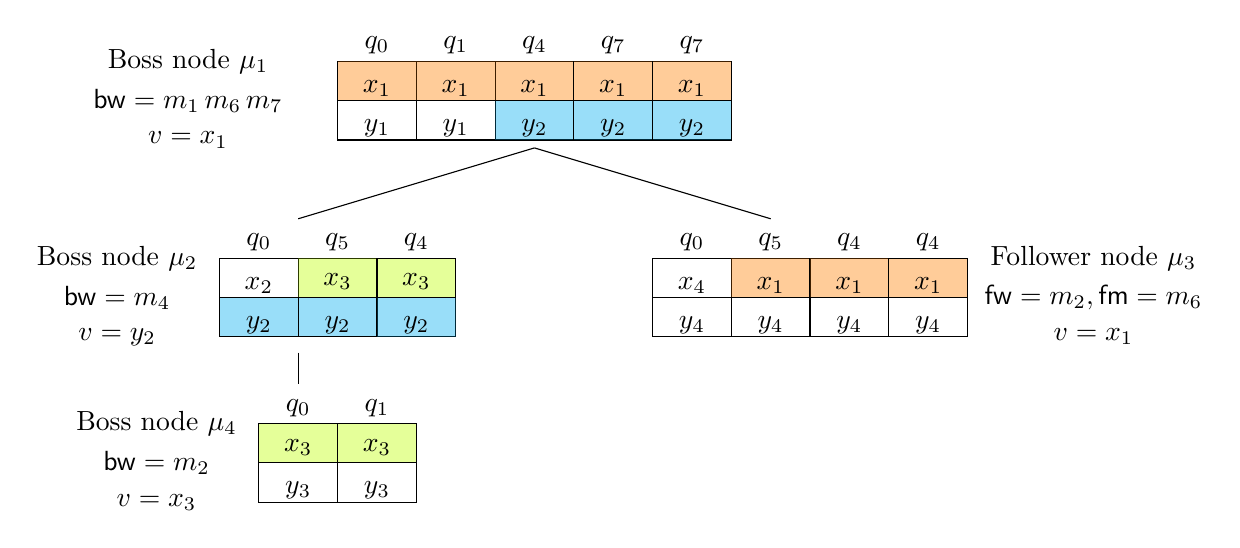
\begin{tikzpicture}
	
	

%	
%	\tikzabstractconfig{0}{0}{$x_1$}{$y_1$}{$q_0$}
%	\tikzabstractconfig{1}{0}{$x_1$}{$y_1$}{$q_1$}
%	\tikzabstractconfig{2}{0}{$x_1$}{$y_2$}{$q_4$}
%	\tikzabstractconfig{3}{0}{$x_1$}{$y_2$}{$q_6$}
	\node [] (sp) at (-2.4, 0.5) {Boss node $\node_1$};
	\node [] (sp) at (-2.4, 0) {$\bossspec = m_1 \, m_6 \, m_7$};
	\node [] (sp) at (-2.4, -0.5) {$v = x_1$};

	\draw (-0.5,0) rectangle (0.5,0.5);
	\draw[fill = orange, opacity=0.4]  (-0.5,0) rectangle (0.5,0.5);
	\draw (-0.5,-0.5 ) rectangle (0.5 ,0);
	\node[] (x1) at (0, 0.15) {$x_1$};
	\node[] (x2) at (0 , 0.15- 0.5) {$y_1$};
	\node [] (q) at (0 , 0.7) {$q_0$};
	
	\draw (0.5,0) rectangle (1.5,0.5);
	\draw[fill = orange, opacity=0.4]  (0.5,0) rectangle (1.5,0.5);
	\draw (0.5,-0.5 ) rectangle (1.5 ,0);
	\node[] (x1) at (1, 0.15) {$x_1$};
	\node[] (x2) at (1 , 0.15- 0.5) {$y_1$};
	\node [] (q) at (1 , 0.7) {$q_1$};
	
	\draw (1.5,0) rectangle (2.5,0.5);
	\draw[fill = orange, opacity=0.4] (1.5,0) rectangle (2.5,0.5);
	\draw (1.5,-0.5 ) rectangle (2.5 ,0);
	\draw[fill = cyan, opacity=0.4] (1.5,-0.5 ) rectangle (2.5 ,0);
	\node[] (x1) at (2, 0.15) {$x_1$};
	\node[] (x2) at (2 , 0.15- 0.5) {$y_2$};
	\node [] (q) at (2 , 0.7) {$q_4$};
	
	
	\draw[] (2.5,0) rectangle (3.5,0.5);
	\draw[fill = orange, opacity=0.4] (2.5,0) rectangle (3.5,0.5);
	\draw (2.5,-0.5 ) rectangle (3.5 ,0);
	\draw[fill = cyan, opacity=0.4]  (2.5,-0.5 ) rectangle (3.5 ,0);
	\node[] (x1) at (3, 0.15) {$x_1$};
	\node[] (x2) at (3 , 0.15- 0.5) {$y_2$};
	\node [] (q) at (3 , 0.7) {$q_7$};

	\draw[] (3.5,0) rectangle (4.5,0.5);
	\draw[fill = orange, opacity=0.4] (3.5,0) rectangle (4.5,0.5);
	\draw (3.5,-0.5 ) rectangle (4.5 ,0);
	\draw[fill = cyan, opacity=0.4]  (3.5,-0.5 ) rectangle (4.5 ,0);
	\node[] (x1) at (4, 0.15) {$x_1$};
	\node[] (x2) at (4 , 0.15- 0.5) {$y_2$};
	\node [] (q) at (4 , 0.7) {$q_7$};
	
    \draw (2, -0.6) -- (-1, -1.5);
    \draw (2, -0.6) -- (5, -1.5);
    
    
    
    \node [] (sp) at (-3.3, 0.7-2.5-0.2) {Boss node $\node_2$};
    \node [] (sp) at (-3.3, 0.7-2.5-0.2-0.5) {$\bossspec = m_4$};
    \node [] (sp) at (-3.3, 0.7-2.5-0.2-1) {$v = y_2$};
    
    \draw (-2,-2.5) rectangle (-1,-2);
    \draw  [fill = cyan, opacity=0.4] (-2,-3 ) rectangle (-1 ,-2.5);    
    \draw  (-2,-3 ) rectangle (-1 ,-2.5);
    \node[] (x1) at (-1.5, 0.15 - 2.5) {$x_2$};
    \node[] (x2) at (-1.5 , 0.15- 0.5 - 2.5) {$y_2$};
    \node [] (q) at (-1.5 , 0.7 - 2.5) {$q_0$};
    
    \draw (-1,-2.5) rectangle (0,-2);
     \draw [fill = lime, opacity=0.4] (-1,-2.5) rectangle (0,-2);
    \draw [fill = cyan, opacity=0.4] (-1,-3 ) rectangle (0 ,-2.5);    
    \draw (-1,-3 ) rectangle (0 ,-2.5);
    \node[] (x1) at (-0.5, 0.2 -2.5) {$x_3$};
    \node[] (x2) at (-0.5 , 0.15- 0.5 - 2.5) {$y_2$};
    \node [] (q) at (-0.5 , 0.7-2.5) {$q_5$};
    
    \draw [fill = lime, opacity=0.4] (0,-2.5) rectangle (1,-2);
    \draw (0,-2.5) rectangle (1,-2);
    \draw (0,-3 ) rectangle (1 ,-2.5);
    \draw[fill = cyan, opacity=0.4] (0,-3 ) rectangle (1 ,-2.5);
    \node[] (x1) at (0.5, 0.2 -2.5) {$x_3$};
    \node[] (x2) at (0.5 , 0.15- 0.5 - 2.5) {$y_2$};
    \node [] (q) at (0.5 , 0.7-2.5) {$q_4$};
    
    
    \draw (-1, -3.2) -- (-1, -3.6);
    
   
   \node [] (sp) at (-2.8, 0.7-4.6-0.2) {Boss node $\node_4$};
    \node [] (sp) at (-2.8, 0.7-4.6-0.2-0.5) {$\bossspec = m_2$};
   \node [] (sp) at (-2.8, 0.7-4.6-0.2-1) {$v = x_3$};
   
   
   \draw (-1.5,-4.6) rectangle (-0.5,-4.1);
   \draw [fill = lime, opacity=0.4] (-1.5,-4.6) rectangle (-0.5,-4.1);
   \draw (-1.5,-5.1 ) rectangle (-0.5 ,-4.6);
   \node[] (x1) at (-1, 0.2 -4.6) {$x_3$};
   \node[] (x2) at (-1 , 0.15- 0.5 - 4.6) {$y_3$};
   \node [] (q) at (-1 , 0.7-4.6) {$q_0$};
    
    
    \draw (-0.5,-4.6) rectangle (0.5,-4.1);
    \draw [fill = lime, opacity=0.4] (-0.5,-4.6) rectangle (0.5,-4.1);
    \draw (-0.5,-5.1 ) rectangle (0.5 ,-4.6);
    \node[] (x1) at (0, 0.2 -4.6) {$x_3$};
    \node[] (x2) at (0 , 0.15- 0.5 - 4.6) {$y_3$};
    \node [] (q) at (0 , 0.7-4.6) {$q_1$};
	
%	\draw (-3,-2) rectangle (-2,0.5 -2);
%	\draw (-3,-0.5 -2) rectangle (1 -3 ,-2);
	%\node[] (x1) at (0.5 + #1, 0.15 +#2) {#3};
	%\node[] (x2) at (0.5 +#1 , 0.15- 0.5 +#2
%	
%	\tikzabstractconfig{-3}{-2}{$x_1$}{$y_1$}{$q_0$} 
%	\tikzabstractconfig{-2}{-2}{$x_1$}{$y_1$}{$q_1$}
	
	
	\draw (3.5,-2.5) rectangle (4.5,-2);
	\draw (3.5,-3 ) rectangle (4.5 ,-2.5);
	\node[] (x1) at (4, 0.15 - 2.5) {$x_4$};
	\node[] (x2) at (4 , 0.15- 0.5 - 2.5) {$y_4$};
	\node [] (q) at (4 , 0.7 - 2.5) {$q_0$};
	
	\draw (4.5,-2.5) rectangle (5.5,-2);
	\draw[fill = orange, opacity=0.4]  (4.5,-2.5) rectangle (5.5,-2);
	\draw (4.5,-3 ) rectangle (5.5 ,-2.5);
	\node[] (x1) at (5, 0.15 - 2.5) {$x_1$};
	\node[] (x2) at (5 , 0.15- 0.5 - 2.5) {$y_4$};
	\node [] (q) at (5 , 0.7 - 2.5) {$q_5$};

	\draw (5.5,-2.5) rectangle (6.5,-2);
	\draw[fill = orange, opacity=0.4] (5.5,-2.5) rectangle (6.5,-2);
	\draw (5.5,-3 ) rectangle (6.5 ,-2.5);
	\node[] (x1) at (6, 0.15 - 2.5) {$x_1$};
	\node[] (x2) at (6 , 0.15- 0.5 - 2.5) {$y_4$};
	\node [] (q) at (6 , 0.7 - 2.5) {$q_4$};
	
	\draw[fill = orange, opacity=0.4] (6.5,-2.5) rectangle (7.5,-2);
	\draw (6.5,-2.5) rectangle (7.5,-2);
	\draw (6.5,-3 ) rectangle (7.5 ,-2.5);
	\node[] (x1) at (7, 0.15 -2.5) {$x_1$};
	\node[] (x2) at (7 , 0.15- 0.5 - 2.5) {$y_4$};
	\node [] (q) at (7 , 0.7-2.5) {$q_4$};
	
	\node [] (sp) at (9.1, -2) {Follower node $\node_3$};
	\node [] (sp) at (9.1, -2.5) {$\followwordspec = m_2, \followmessagespec= m_6$};
	\node [] (sp) at (9.1, -3) {$v = x_1$};
	
%	\draw (7.5,-2.5) rectangle (8.5,-2);
%	\draw (7.5,-3 ) rectangle (8.5,-2.5);
%	\node[] (x1) at (8, 0.2 -2.5) {$x'_2$};
%	\node[] (x2) at (8 , 0.15- 0.5 - 2.5) {$y_2$};
%	\node [] (q) at (8 , 0.7-2.5) {$q_4$};
%	
\end{tikzpicture}
				% }
		\end{center}
	\vspace*{-0.5cm}
	\caption{Example of an "unfolding tree". $\delta_{ri}$ (resp. $\delta_{bi}$) denotes the reception (resp. broadcast) transition of message $m_i$ in the protocol described in \cref{fig:ex1}. Initial values which are never broadcast are omitted and written as $\quotemarks{\_}$.}\label{fig:ex-unfolding-tree}
%	\vspace*{-0.5cm}
\end{figure}

A ""coverability witness"" is again an "unfolding tree" whose root covers $q_f$, with the extra condition that the root is a "boss node" (a "follower node" implicitely relies on its parent's ability to broadcast). 

\begin{restatable}{proposition}{treessoundcomplete}
	\label{prop:trees-sound-complete}
	An instance of \COVER $(\prot,q_f)$ is positive if and only if there exists a "coverability witness" for that instance.
\end{restatable}
\begin{proof}[Proof sketch]
	The proof is quite similar to the one of Lemma~\ref{lem:coverability_witness_sg}, but is made more technical by the addition of "follower" nodes. 
	When translating an "unfolding tree" to a "run", if the root of the tree is a "follower node" $\node$ of specification $(\followwordspec, \followmessagespec)$, then we actually obtain a "partial run", \emph{i.e.}, a "run" except that the receptions from $\followwordspec$ are not matched by broadcasts in the "run". We then need to interleave the runs of the parent of $\node$ with (several copies of) its follower children, as detailed in Lemma~\ref{lem:tree-to-run-technical}.
	For the translation from "run" to tree, we inductively construct the tree by extracting from the run the agents and values responsible for satisfying the specifications of each node and analysing the messages they receive to determine their set of children (as in Example~\ref{ex:decomposition}). See Appendix~\ref{app:trees-sound-complete} for the proof.
%	\corto{A relire} 
	% % The translation from "run" to tree works by induction on the length of the "run". We first define in a natural way what it means for a "run" to satisfy a "specification". We consider a "run" $\run$ and isolate a well-chosen agent $a$, whose "local run" witnesses that the "specification" is satisfied. We call the induction hypothesis with the "specifications" expressing what $a$ needs to receive from other agents. Each such "specification" is satisfied by a strict prefix of $\run$ (the only exception being if $a$ satisfies a "boss specification" with value $v$ and the last step of $\run$ is a broadcast with $v$ by another agent; in this case, we use the induction hypothesis on $\run$ but with a follower specification, hence the induction is well-founded).
	% We construct an "unfolding tree" by labeling the root with the "specification" and the "local run" of $a$, and attaching below it the subtrees obtained by induction hypothesis.
	% The translation from tree to "run" consists in an induction on the tree. A key concept is the one of "partial run", which extends the notion of "local run" to a subset of agents: in a "partial run", some receptions called \emph{external} are not matched by a broadcast. This is meant to represent the behavior of a subtree of the "unfolding tree": if the root of an "unfolding tree" is a "follower node" with "specification" $(\followwordspec, \followmessagespec)$ then the corresponding "partial run" receives an external sequence $\followwordspec$. The inductive step applies the induction hypothesis to the children of the "root" to obtain partial runs and merges them with the "local run" of the root by branching broadcasts to the right external receptions. 
	% 
\end{proof}





\subsubsection{Bounding the Size of the Unfolding Tree.}
\label{sec:tree-bounds}

Our aim is again to bound the "size@@tree" of a minimal "coverability witness". In the following, we fix an instance $(\prot,q_f)$ with $r$ registers and a "coverability witness" of minimal size. We start by providing new conditions under which a branch can be shortened; for "boss specifications", it is the condition of Lemma~\ref{lem:no_subword_in_branch_sg} but for "follower specifications", the subword relation goes the opposite direction because the shorter the requirement $\followwordspec$, the better.

\begin{restatable}{lemma}{lemShorteningBranches} 
\label{lem:shortening-branches}
	Let $\node \ne \node'$ be two nodes of $\tree$ such that $\node$ is an ancestor of $\node'$. If one of those conditions holds, then $\tree$ can be shortened  (contradicting its minimality):
	\begin{itemize}
	\item $\node$ and $\node'$ are "boss nodes" and $\bosslabel{\node} \subword \bosslabel{\node'}$; 
	\item $\node$ and $\node'$ are "follower nodes", $\followlabelword{\node'} \subword \followlabelword{\node}$ and $\followlabelmessage{\node'}=\followlabelmessage{\node}$.
	\end{itemize} 
\end{restatable}

We can generalize \cref{lem:towerbound_signature} to bound the size of a node by the number of messages that it must broadcast times a primitive-recursive function $\towerfun(\size{\prot},r)$. The proof is more technical than the one of \cref{lem:towerbound_signature} but the idea is essentially the same. The formal statement and the proof can be found in Appendix~\ref{app:tower-lemma} (\cref{lem:short-local-runs}). 
One can therefore bound the size of a node with respect to the size of the nodes that it must broadcast to.

It is however much harder to bound the size of the "coverability witness" in the general case than it was in the "signature" case. Indeed, the broadcasts no longer go only from children to parents in the "unfolding tree". If $\node$ is the parent of $\node'$, then $\node'$ broadcasts to $\node$ if $\node'$ is a "boss node", but $\node$ broadcasts to $\node'$ if $\node'$ is a "follower node", in which case $\node'$ only broadcasts one message to $\node$. Therefore, we cannot in general bound $\size{\node}$ with respect to $\size{\node'}$ nor $\size{\node'}$ with respect to $\size{\node}$, making us unable to apply the "Length function theorem" immediately. 

This leads us to arrange the "unfolding tree" so that long broadcast sequences are sent upwards, using the notion of "altitude" depicted in Figure~\ref{fig:rearrange-tree}, formally defined as follows:

The ""altitude"" of the root is $0$, the altitude of a "boss node" is the altitude of its parent minus one, and the altitude of a "follower node" is the altitude of its parent plus one.
We denote the "altitude" of $\node$ by $\altitude{\node}$.
This way the nodes of maximal "altitude" are the ones that do not need to send long sequences of messages. We will bound the size of nodes with respect to their "altitude", from the highest to the lowest, and then use the "Length function theorem" to bound the maximal and minimal "altitudes".


% note that this time the bound is on the exact number of registers (and not the number of registers minus one). We shall refer to this lemma as the Tower Function Lemma as it bounds "local runs" length by a function $\psi(n,k)$ which is in fact a tower of exponentials of height $k$ where each floor is a polynomial in $n$.

% Previously, \cref{lem:no_subword_in_branch_sg,lem:towerbound_signature} lead us to the "Length function theorem". We were able to bound the size of a node with respect to the nodes to which it must send long words of messages (in the signature protocol: from leaves to root), i.e. we could find a bound for a node $\node$ with respect to its parent's size. From what we argued above, we can not do so in the general case.
%However, this is not possible for "follower nodes", as it goes in the opposite direction: a node now might need to send long sequence of messages to its "follower node" child, in order for this node to repeat a value. 
% We will thus rearrange the tree in a convenient manner. 

% A new version of \cref{lem:no_subword_in_branch_sg} can be found below: \cref{lem:shortening-branches} provides two ways of shortening an "unfolding tree", its proof can be found in Appendix~\ref{app:proofs-reduction-branches}. 
%and \cref{lem:short-local-runs}~is the direct general case version of \cref{lem:towerbound_signature}.






%\cref{lem:no_subword_in_branch_sg} is then replaced by the following lemma, which 





%We now show that there is a computable bound on the "size@@tree" of the "unfolding tree" achieving a given specification and labeled with a "protocol" $\prot$. Lemma~\ref{lem:shortening-branches} leads us towards an application of the "Length function theorem"; however, this theorem requires a bound on the lengths of the words. In fact, there is no reason to think that the lengths of the labels of the children of a node can be bounded with respect to the length of the label of that node. 
%
%
%In order to bound the size of the nodes, we now wish to adapt \cref{lem:towerbound_signature}~to the general case.
%We use the following result, which essentially states that if there is a "local run" between two local configurations $(q, \nu)$ and $(q', \nu')$ then there is one of length bounded by a primitive recursive function and which does not require larger inputs than the previous one.

%\begin{restatable}{lemma}{lemShortLocalRuns}
%	\label{lem:short-local-runs}
%	There exists a primitive recursive function $\towerfun(n,r)$ such that, for every "protocol" with $r$ registers, for every local run $\localrun: (q,\localdata) \step{*} (q', \localdata')$, there exists $u' : (q,\localdata) \step{*} (q',\localdata')$ such that $\size{u'} < \towerfun(\size{\prot},r)$ and for all value $v \in \nats$,  $\vinput{v}{u'} \subword \vinput{v}{u}$. 
%%	\\
%%	
%%	There exists a primitive recursive function $\towerfun(n,r)$ such that, for every protocol $\prot$ with $r$ registers, for every "local run" $\localrun_0: (q_0, \localdata_0) \step{*} (q_f, \localdata_f)$ in $\prot$, for every section $\localrun : (q, \localdata) \step{*} (q, \localdata')$ of $\localrun_0$,  for every $V \subseteq \nats$ finite such that $V$ contains all message values appearing in $\localrun$, there exists a "local run" $\localrun': (q, \localdata) \step{*} (q', \localdata')$ such that we have $\length{\localrun''} \leq \towerfun(\size{\prot},r)$ and:
%%	\begin{enumerate}
%%		\item for all $\aval' \in \nats \setminus V$, there exists $\aval$ a "non-initial" value of $\localrun_0$ such that $\vinput{\aval'}{\localrun'}\subword \vinput{\aval}{\localrun}$,
%%		\item for all $\aval \in V$, $\vinput{\aval}{\localrun'} \subword \vinput{\aval}{\localrun}$. 
%%	\end{enumerate}
%\end{restatable}
%
%\begin{proof}[Proof sketch]
%	
%	
%	The proof follows the same reasoning as the proof of \cref{lem:towerbound_signature}, but this time all registers should be taken into consideration.
%	\luin{pour le moment j'ai juste déplacé l'ancien énoncé en annexe, vérifier si on peut adapter le lemme tower "signé" et sa preuve plus simplement}
%	
%%	First, as for \cref{lem:towerbound_signature}, we prove that any long portion of $\localrun$ must change the value of every register at least once; otherwise we can shorten the "run" using an induction on the number of registers. We then manage to prove that, if $\localrun$ includes twice the same sequence of transitions of sufficient length, then we can cut off anything in the middle and glue back together the ends. While shortening the "local run" we may add some fresh values to it (see Figure~\ref{fig:pumping} in the appendix), which is not a problem as we ensure that they are less constraining than the ones that were in the original "run". For technical reasons, we want to prevent fresh values added in the proof from mimicking "initial" values of the agent.\lu{je crois que c'est pour les local disequality tests qui ne sont plus là désormais, à enlever?}
%%	See Appendix~\ref{app:tower-lemma} for the full proof.
%	
%	

% Perhaps surprinsingly, this bound is tight: one may need a "local run" of length a tower of exponentials to reach a given "local configuration" while being allowed to receive sequences of messages of same value from a given fixed set. 
%\begin{remark}\lu{déplacer si manque de place ?}
%	The function $\towerfun(n,k)$ defined above is actually a tower of exponentials of height $k$ where each floor is a polynomial in $n$. Perhaps surprinsingly, this bound is tight: one may need a "local run" of length a tower of exponentials to reach a given "local configuration" while being allowed to receive sequences of messages of same value from a given fixed set. 
%\end{remark}

% \begin{remark}
% 	The function $\towerfun$ above is a tower of exponentials of height $\regnum$. Perhaps surpringly, this tower bound is tight in the sense that one can find a family of protocols and of "local runs" such that the best $\towerfun$ possible is a tower of exponentials of height linear in $\regnum$. Suppose that we have a protocol $\prot$ and a state $q_f$ such that $q_f$ may only be reached by going exactly $N$ times through some state $q_r$. From $\prot$, we build a "protocol" $\prot'$ with two extra registers $r_0$ and $r_1$; $\prot'$ uses $\prot$ to consider sequences of messages of length $N$ (duplicate $q_r$ into $q_r'$ and $q_r''$ and add transitions in between). Words received by $r_0$ and $r_1$ are of length $N$ with the same value, we see those as binary encodings using $\mathsf{0}, \mathsf{1} \in \messages$. $\prot'$ first requires that $r_0$ receives a word of length $N$ encoding $0$, then iteratively requires that $r_{1-i}$ receives a message encoding value $m+1$ where $m$ is the value last received in $r_i$ (to be able to compare, the words received are of the form $w \#w$ with $w$ of length $N$; the comparison requires to be able to store the value of $i$, whether there is a carry,... which can be done using a third register to avoid a multiplicative factor between sizes of $\prot$ and $\prot'$). We only cover $q_f'$ when word $\mathsf{1}^N$ is received, which is only possible after going exactly $N'$ times through $q_r'$ steps with $N'$ exponential in $N$.
% \end{remark}
%\begin{definition}
%	Let $\tree$ an "unfolding tree". We define the ""altitude"" of a node $\node$ of $\tree$, written $\altitude{\node}$, recursively as follows:
%	\begin{itemize}
%		\item The altitude of the root is $0$,
%		\item The altitude of a "boss node" is the altitude of its parent minus one,
%		\item The altitude of a "follower node" is the altitude of its parent plus one.
%	\end{itemize}
%\end{definition}

\begin{figure}[t]
	
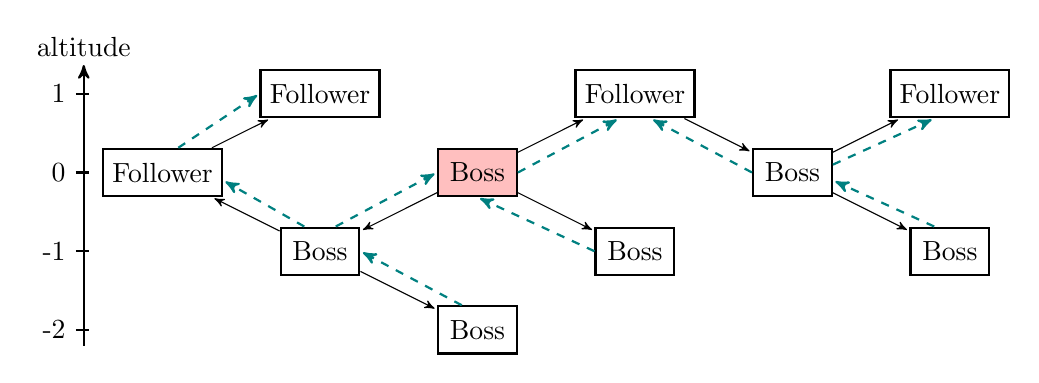
\begin{tikzpicture}[ >=stealth', shorten >=1pt,node distance=2cm,on grid, initial text = {}] 
	
	\tikzset{
		tnode/.style = {rectangle, draw, thick, minimum width=1cm,
			minimum height = 0.6cm}
	}



%	\begin{axis}[
%		xmin = -2,
%		xmax = 1,
%		grid = both,
%		grid style = {
%			line width=.1pt, 
%			draw=gray!10},
%		major grid style = {
%			line width = 0.2pt,
%			draw = gray!50},
%		axis lines = middle,
%		minor tick num = 0, % à changer pour plus de subdivisions
%		enlargelimits = { abs = 0 },
%		axis line style = {-},
%		ticklabel style = {
%			font = \tiny,
%			fill = white},
%		xlabel style = {
%			at = {(ticklabel* cs:1)},
%			anchor = north west
%		},
%		ylabel style = {
%			at = {(ticklabel* cs:1)},
%			anchor = south west
%		}
%		]

	\draw[black, ->, thick](-5,-2.2)--(-5,1.4);
	\node[black, thick] at (-5,1.6) {altitude};
	\foreach \y in {-2,...,1} \draw[black, thick] (-5.1, \y )node[left, thick]{\y} -- (-4.9, \y);
	
	 \node[tnode, fill=pink!] (root) { Boss};
	 \node[tnode] (n1) [above = 1cm of root, xshift = 2cm]{ Follower};
	 \node[tnode] (n2) [below = 1cm of root, xshift = 2cm]{ Boss};
	 \node[tnode] (n3) [right = 4cm of root]{ Boss};
	 \node[tnode] (n4) [above = 1cm of n3, xshift = 2cm]{ Follower};
	 \node[tnode] (n5) [below = 1cm of n3, xshift = 2cm]{ Boss};
%	 \node[tnode] (n6) [below = 3cm of root]{ $\bossspec$};
%	\node[tnode] (n7) [above = 2.6cm of root]{ $(\followwordspec, \followmessagespec)$};
%	\node[tnode] (n8) [above = 1cm of n4, xshift = -2cm]{ $(\followwordspec, \followmessagespec)$};

	
	\node[tnode] (m1) [below = 1cm of root, xshift = -2cm]{ Boss};
	\node[tnode] (m2) [above = 1cm of m1, xshift = -2cm]{Follower};
	\node [tnode] (m3) [above = 1cm of m2, xshift = 2cm] {Follower};
	\node[tnode] (n9) [below = 1cm of m1, xshift = 2cm]{ Boss};
	
	
	\path[->]
	(root) edge [ ]  node {} (n1)
				edge node {} (n2)
				edge [ ] node {} (m1)
	(n1) edge node {} (n3)
	(n3) edge node {}  (n4)
			edge node {}   (n5)
			
	(m1) edge node {} (m2)
	(m2) edge node {} (m3)
%	(n4) edge [  ] node {} (n8) 
	(m1) edge [ ] node {} (n9)
	;
	
	
		\path[->, dashed, teal, thick] 
		(root.east) edge node {} ([xshift = -0.2cm]n1.south)
		(n2.west) edge node {} (root.south)
		([xshift = 0.2cm]m1.north) edge node {} (root.west)
		(n3.west) edge node {} ([xshift = 0.2cm]n1.south)
		([yshift = 0.1cm]n3.east) edge node {} ([xshift = -0.2cm]n4.south)
		 
		([xshift = -0.2cm]n5.north) edge node {}  ([yshift = -0.1cm]n3.east) 
%		([yshift = 0.1cm]n4.west) edge node {} ([xshift = 0.2cm]n8.south)
		
		([xshift = -0.2cm]m1.north) edge node {} ([yshift = -0.1cm]m2.east)
		([xshift = 0.2cm]m2.north) edge node {} (m3.west)
		 ([xshift = -0.2cm]n9.north) edge node {} (m1.east) 
		;
		
%		\path[->, dashed, teal] 
%		 ([xshift = -0.2cm]n1.south) edge node {} (root.east)
%		(root.south) edge node {} (n2.west)
%		(root.west) edge node {} ([xshift = 0.2cm]m1.north)
%		([xshift = 0.2cm]n1.south) edge node {} (n3.west)
%		([xshift = -0.2cm]n4.south) edge node {} ([yshift = 0.1cm]n3.east) 
%		([yshift = -0.1cm]n3.east) edge node {}   ([xshift = -0.2cm]n5.north)
%		([xshift = 0.2cm]n8.south) edge node {} ([yshift = 0.1cm]n4.west) 
%		
%		([yshift = -0.1cm]m2.east) edge node {} ([xshift = -0.2cm]m1.north)
%		(m3.west) edge node {} ([xshift = 0.2cm]m2.north)
%		(m1.east) edge node {} ([xshift = -0.2cm]n9.north)
%		;

	    %\draw[>={Stealth[round,sep]}](n8) --  (n7);
	
%	  \draw [->, red, thick, dotted] (n8) -- (n7);
%	  \draw[->, blue, thick, dotted] (n9) -- (n6);
	
	
	
\end{tikzpicture}
	\caption{Rearrangement of a tree. The root is in red, black solid arrows connect parents to children, blue dashed arrows highlight that long words of messages are sent upwards.}
	\label{fig:rearrange-tree}
\end{figure}

We bound the size of a node with respect to the size of its neighbors of higher altitude.

\begin{restatable}{lemma}{lemBoundSuccessorHeight}
	\label{lem:bound-successor-height}
	Let $\node$ be a node of $\tree$ such that all neighbors of $\node$ of higher altitude have size bounded by $K$.
	Then $\size{\node} \leq (\towerfun(\size{\prot}, r)+2) \, (\size{\messages} \, r \, K + K)$, with $\psi$ the primitive-recursive function defined in Lemma~\ref{lem:short-local-runs}. 
\end{restatable}

\begin{proof}
	The idea is similar to the one for Lemma~\ref{lem:bounds_tree_sg}. The neighbors of higher "altitude" are the nodes which require sequences of messages from $\node$. Their size bounds the number of messages that this node needs to send, and then we can apply Lemma~\ref{lem:short-local-runs} (which generalizes Lemma~\ref{lem:towerbound_signature}) to bound the local run of the node.
	The full proof can be found in Appendix~\ref{app:proofs_bounds}.
\end{proof}

The rest of the proof is sketched here and detailed in Appendix~\ref{app:proofs_bounds}. 
By inductively applying the previous result, we obtain the existence of a primitive-recursive function $f_0$ (depending only on $\size{\prot}$ and not on $\tree$) such that, given a node $\node$ in $\tree$, $\size{\node} \leq f_0(\altmax - \altitude{\node})$ where $\altmax$ denotes the maximal altitude in $\tree$ (Lemma~\ref{lem:bound-length-at-height-h}).

We now bound $\altmax$. Consider a branch of $\tree$ with a node at "altitude" $\altmax$; we follow this branch from the root and, for every $j \in \nset{1}{\altmax}$, set $\node_{j}$ as the first node of the branch at altitude $j$ (Figure~\ref{fig:max-height-bound} in the appendix); all such nodes are necessarily "follower nodes" as they are above their parent. Sequence $\node_{\altmax}, \dots, \node_2, \node_1$ is so that the $i$th term is at altitude $\altmax-i$ hence its size is bounded by $f_0(i)$. With the observation of Lemma~\ref{lem:shortening-branches}, we apply the "Length function theorem" to bound $\altmax$ (Lemma~\ref{lem:bound-max-height} in the appendix).

This yields in turn a bound on the size of the root of $\tree$ as its altitude ($0$) has a bounded difference with the maximal one. Another application of the "Length function theorem", this time with "boss nodes", allows us to bound the minimal altitude of a node of this tree (Lemma~\ref{lem:bound-min-height}).
	
Once we have bounded both the maximal and minimal altitudes, we can infer a bound on the size of all nodes using Lemma~\ref{lem:bound-length-at-height-h}, and then on the length of branches: by minimality, a branch cannot have two nodes with the same specification. 
The bound on the "size@@tree" of the tree then follows from the observation that bounding the size of nodes of $\tree$ also allows to bound their number of children.
 

% \begin{restatable}{proposition}{PropBoundTreeSize}
% 	\label{prop:bound-tree-size}
% 	There exists a function $f$ of class $\Ffunction{\omega^{\size{\messages}+1}}$ s.t. $\size{\tree} \leq f(\size{\prot})$.
% \end{restatable}

%\subsubsection{Decidability}
%\label{sec:decidability-end}

We obtain a computable bound (of the class $\Ffunction{\omega^\omega}$) on the "size@@tree" of a minimal "coverability witness", if it exists. 
Our decidability procedure computes that bound, enumerates all trees of "size@@tree" below the bound and checks for each of them whether it is "coverability witness". Details can be found in Appendix~\ref{app:proofs_bounds} and Appendix~\ref{app:decidable_cover}.

\decidablecover*



%	\subsection{Undecidability of \Target}
\label{sec:undec-target}

The "target reachability problem" is a natural next step after coverability. 
It requires a more precise description of runs: while for \COVER we can produce a lot of waste, in the sense that we can add as many agents as we need to ensure that one of them reaches the given state, for \Target we need to guarantee that those agents can later reach the target state.

We show that \Target is undecidable for BNRAs, which suggests that while we can obtain decidability of \COVER thanks to the monotonicity of the problem, we cannot analyse precisely the set of runs of such systems.


\begin{restatable}{proposition}{propTargetUndecidable}
\label{prop:target-undec}
	The "target reachability problem" (asking whether there is a run in which all agents reach a state $q_f$) is undecidable for \BNRA with two registers.
\end{restatable}

The proof goes as follows: We simulate a Minsky machine with two counters. In an initialisation phase, all agents record a value  sent by another agent in their second register, which will be their ``predecessor''. Throughout the run they will only listen to broadcasts from that agent, and only broadcast with the initial value in their first register. As there are finitely many agents, there must be a cycle in the predecessor graph.

We exploit the fact that \textbf{all} agents must reach state $q_f$ to simulate faithfully a Minsky machine: we make agents alternate between receptions and broadcasts so that in the end they have received and sent the same number of messages, implying that all messages have been received along the cycle.

Once we guarantee that no messages are lost, we can simulate the machine by having an agent (the leader) choose transitions of the machine and the other ones simulate the counter values by memorizing a counter 1 or 2 and a bit 0 or 1. For instance, an increment of counter 1 is done by having the leader send a message around the cycle, which eventually finds an agent simulating counter 1 and with bit 0, which switches to 1 and sends a confirmation message to confirm to the leader that the operation has been executed.
	\section{Cover in 1-BNRAs}
	\label{sec:cover-1BNRA}
	\section{Definitions}

\begin{definition}
	A ""protocol"" is a tuple $\prot = (Q, \messages, \transitions, q_0)$  with $Q$ a finite set of states, $q_0 \in Q$ an initial state, $\messages$ a finite set of ""messages""  and $\transitions \subseteq Q \times \set{\br{\amessage}, \rec{\amessage}{\dummyact}, \rec{\amessage}{\enregact}, \rec{\amessage}{\eqtestact}, \rec{\amessage}{\diseqtestact} \mid \amessage \in \messages} \times Q$.
	
	Transitions labelled with $\brsymb$ are ""broadcasts"" and transitions labelled with $\recsymb$ are ""receptions"".
Given a reception $(q,\rec{\amessage}{\anact}, q') \in \transitions$, $\anact$ is the ""action"" of the reception.
\end{definition}

\begin{definition}
	Let $(Q,\messages, \transitions, q_0)$ be a protocol, and $\agents \subseteq \nats$ a finite set of \emph{agents}.
	A ""configuration"" over a set of agents $\agents$ is a labelling function $\config : \agents \to Q \times \nats$, associating a state and a ""register value"" to each agent. We write $\st{\config}$ for the state component of $\config$ and $\data{\config}$ for its register component. 
	An \emph{initial configuration} $\config$ is one where for all $a \in \agents$, $\st{\config}(a) = q_0$ and for all $a, a' \in \agents$, if $\data{\config}(a) = \data{\config}(a')$ then $a=a'$.
	
	\AP We denote by $\configs{\agents}$ the set of configurations over $\agents$, and by $\allconfigs := \cup_{\agents \subseteq \nats \text{ finite }} \configs{\agents}$ the set of all configurations. Given a configuration $\config$, we denote by $\agentsof{\config}$ the set of agents of $\config$.

	\AP Given two configurations $\config, \config' \in \configs{\agents}$, a ""step"" $\config \step{} \config'$ is defined when there exists $\amessage \in \messages$ and $a_0 \in \agents$ such that $(\st{\config}(a_0),\br{\amessage}, \st{\config'}(a_0)) \in \transitions$, $\data{\config}(a_0) = \data{\config'}(a_0)$ and for all $a \in \agents\setminus \set{a_0}$,  
	\begin{itemize}
		\item either $\config'(a) = \config(a)$
		
		\item or $\config'(a)$ is such that $(\st{\config}(a), \rec{\amessage}{\anact}, \st{\config'}(a)) \in \transitions$ with either
		\begin{itemize}
			\item $\anact = \quotemarks{\dummyact}$ 
			and $\data{\config'}(a) = \data{\config}(a)$
			\item $\anact = \quotemarks{\enregact}$ and $\data{\config'}(a) = \data{\config'}(a_0)$
			\item $\anact = \quotemarks{\eqtestact}$ and $\data{\config'}(a) = \data{\config}(a) =\data{\config'}(a_0)$
			\item $\anact = \quotemarks{\diseqtestact}$ and $\data{\config'}(a) = \data{\config}(a) \ne \data{\config'}(a_0)$
		\end{itemize}
	\end{itemize}

	\AP A ""run"" is a sequence of steps $\run : \config_0 \step{} \config_1 \step{} \cdots \step{} \config_k$ such that $\config_0$ is an "initial configuration". We write $\config_0 \step{*} \config_k$ the existence of such a "run". Given such a "run" $\run$, we write $\agentsof{\run}$ its set of agents and $\statesin{\run}:= \set{q \in Q \mid \exists i, \exists a, \st{\config_i}(a) = q}$ the set of states appearing in $\run$.  
% with current definition, every run is initial

%We say that it is ""initial@@run"" if $\config_0$ is an initial configuration.
\end{definition}

\begin{definition}
We define a preorder over the set of configurations $\allconfigs$ as follows: $\config \lessthan \config'$ if there exists an injective function $\pi: \agentsof{\config} \rightarrow \agentsof{\config'}$ such that, for all $a \in \agentsof{\config}$, $\config(a) = \config'(\pi(a))$. 
\end{definition}

\begin{definition}
	A ""query"" $\query$ is a finite set of formulas of the form $\quotemarks{q(\var{z})}$, $\quotemarks{R(\var{z}) = R(\var{z}')}$, $\quotemarks{R(\var{z}) \neq R(\var{z}')}$, with $\var{z}, \var{z}'$ taken in a set of variables $\varset$.
	It is \emph{satisfied} by a "configuration" $\config$ if there is a valuation $\nu : \varset \to \agentsof{\config}$ such that:
	\begin{itemize}
		\item for all $\quotemarks{q(\var{z})} \in \query$, $\st{\config}(\nu(\var{z})) = q$,
		
		\item for all $\quotemarks{R(\var{z}) = R(\var{z'})} \in \query$, $\data{\config}(\nu(\var{z})) = \data{\config}(\nu(\var{z'}))$,
		
		\item for all $\quotemarks{R(\var{z}) \neq R(\var{z'})} \in \query$, $\data{\config}(\nu(\var{z})) \neq \data{\config}(\nu(\var{z'}))$.
	\end{itemize}

	\AP The ""query coverability problem"" is to determine, given a "protocol" and a "query", whether there is a "run" of this protocol whose last "configuration" satisfies the query.
\end{definition}

\begin{remark}
\label{rem:bigger_config_query}
If some "configuration" $\config$ satisfies a "query" $\query$, then every configuration $\config'$ such that $\config \lessthan \config'$ satisfies $\query$. 
\end{remark}





	
\luin{exemples + rappel copy cat (sous angle de r = 1) + lemma no diseq}

%\begin{example}\lu{est ce que cet exemple a vraiment sa place dans la version conférence ? j'aurai plutot mis un exemple qui donne une idée de 1) pourquoi c'est plus facile que dans le cas général et/ou 2) pourquoi c'est plus compliqué que le papier de RP }
%	In some cases a protocol may require a "run" of exponential length (in the number of states) to reach a configuration satisfying a "query".
%	
%	\begin{figure}[h]
%		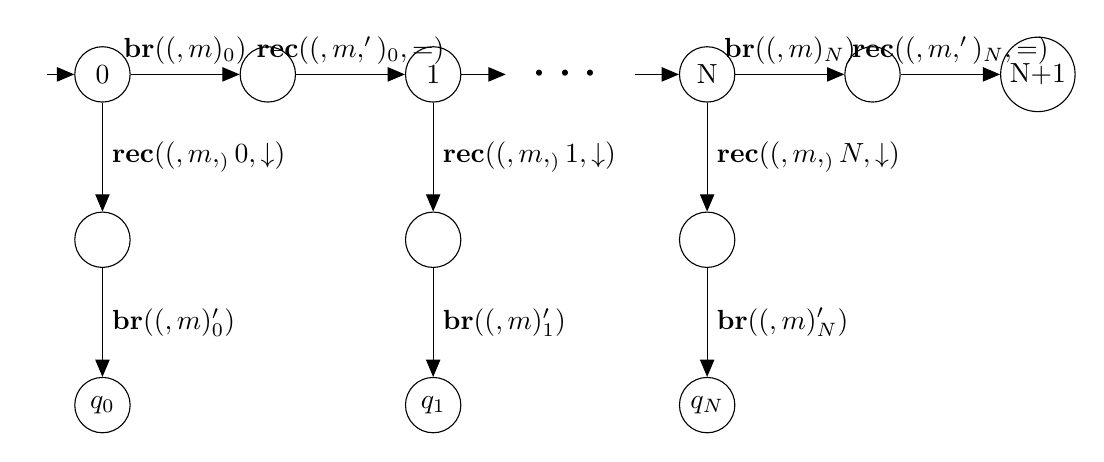
\begin{tikzpicture}[xscale=0.5,AUT style,node distance=2.1cm,auto,>= triangle
	45]
	\tikzstyle{initial}= [initial by arrow,initial text=,initial
	distance=.7cm]
	%	\tikzstyle{accepting}= [accepting by arrow,accepting text=,accepting
	%	distance=.7cm,accepting where =right]
	
	\node[state,initial, minimum width=0.1pt] (0a) at (0,0) {0};
	\node[state] [below of=0a] (0b) {};
	\node[state] [below of=0b] (0c) {$q_0$};
	\node[state] [right of=0a] (0') {};
	
	\node[state] [right of=0'] (1a) {1};
	\node[state] [below of=1a] (1b) {};
	\node[state] [below of=1b] (1c) {$q_1$};
	
	\node [right of=1a, xshift=-30pt] (token1) {};
	\node [right of=token1, xshift=-40pt] (dots) {\huge $\cdots$};
	\node [right of=dots, xshift=-40pt] (token2) {};
	
	\node[state] [right of=token2, xshift=-30pt] (Na) {N};
	\node[state] [below of=Na] (Nb) {};
	\node[state] [below of=Nb] (Nc) {$q_N$};
	
	\node[state] [right of=Na] (N') {};
	\node[state] [right of=N'] (end) {N+1};
	
	\path[->, bend left=20] 	
	;
	\path[->, bend right=20] 
	;
	\path[->]
	(0a) edge node[right] {$\rec(m_0, \enregact)$} (0b)
	(0b) edge node[right] {$\br(m'_0)$} (0c)
	
	(1a) edge node[right] {$\rec(m_1, \enregact)$} (1b)
	(1b) edge node[right] {$\br(m'_1)$} (1c)
	
	(Na) edge node[right] {$\rec(m_N, \enregact)$} (Nb)
	(Nb) edge node[right] {$\br(m'_N)$} (Nc)
	
	(0a) edge node {$\br(m_0)$} (0')
	(0') edge node {$\rec(m'_0, \eqtestact)$} (1a)
	
	(Na) edge node {$\br(m_N)$} (N')
	(N') edge node {$\rec(m'_N, \eqtestact)$} (end)
	
	(1a) edge node {} (token1)
	(token2) edge node {} (Na)
	;
\end{tikzpicture}
%		\caption{Example of a "protocol" with a state that requires an exponentially long "run" to be covered.}
%		\label{fig:exp-run}
%	\end{figure}
%
%	Consider the "protocol" displayed in Figure~\ref{fig:exp-run}. 
%	For all $n \in \set{0, \ldots, N+1}$ we call \emph{future} of $n$ the set of states accessible from state $n$ by a path in the protocol.
%	
%	There is an initial run covering $N+1$: we start with $2^{N+1}$ agents, which we pair two by two. We make each agent broadcast $m_0$ while its partner receives it, storing its register value and broadcasts $m'_0$, which the first one receives. After doing that with all pairs of agents we have $2^{N}$ agents in state $1$.
%	We repeat this process to put $2^{N+1-n}$ agents in state $n$ for each $n$, one after the other. In the end we have an agent in state $N+1$.
%	
%	We show by induction on $n$ that for all $k \in \nats$, any reachable configuration with at least $k$ agents in states of the future of $n$ has at least $k(2^n-1)$ agents in states $\set{q_i \mid i<n}$.
%	
%	For $n=0$ this is immediate. Let $n>0$, suppose the property true for $n-1$, then let $k \in \nats$ and let $\config$ be a configuration with at least $k$ agents in the future of $n$. Let $\agents_+$ be the set of those agents, let $a_+ \in \agents_+$, $a_+$ has taken the transitions broadcasting $m_{n-1}$ and receiving $m'_{n-1}$ with its own register value. As it never changed its identifier, the reception must contain its initial value $r$. Hence there exists an agent $a_-$ which broadcasts $m'_{n-1}$ at some point while having value $r$. All such $a_-$ are distinct as they all broadcast only once with $m'_{n-1}$ and the $a_+$ have distinct initial values.
%	Hence there are at least $k$ agents in state $q_{n-1}$, hence at least $2k$ in the future of $n-1$. By induction hypothesis this means there are $2k(2^{n-1}-1) = k(2^n-2)$ in $\set{q_i \mid i<n-1}$, thus at least $k(2^n-1)$ in $\set{q_i \mid i<n}$.
%	
%	As a consequence, any initial run covering $N+1$ needs to send at least $2^N-1$ agents to the $q_i$ states, hence it needs to be exponentially long as each of those agents needs to execute at least one broadcast.
%\end{example}



	%\subsection{Upper bound}
To prove that the "query coveravility problem" is in NP in the special case where there is only one register\lu{trouver abbréviation pour BNRA+1 reg}, we will present an abstraction on "configurations" and "runs". Intuitively, our abstraction keeps track of a set of reachable states and what we shall name a "gang". A "gang" represents a "boss" state and a set of "followers" states, it should represent all configurations in which a process is on the "boss" state and kept its initial value $v$ and other processes are on the "followers" states with register value $\val$. We will define an abstract semantics, and prove it to be sound and complete. Finally, we will present a NP-algorithm on this abstraction to answer the "query coverability problem".

In order to make proofs easier, and simplify the problem, we first present some preliminaries lemmas which allow us to (i) reduce our analysis to protocols that does not have receptions with actions $\quotemarks{\ne}$, or local tests, (ii) only consider "non-contradictory" queries.

\subsection{Preliminaries}



%\begin{definition}
%	Given two runs $\run, \run'$ over sets of agents $\agents, \agents'$ respectively, we define their ""parallel composition"" as the run over $\agents\times \set{0} \cup \agents'\times \set{1}$ defined as follows: 
%\end{definition}

\cortoin{Copycats are not used in the proofs. Remove?}
\luin{sometimes "copycat principle"}

In this model, given a run, we can clone it. Take a disjoint set of agents, with a disjoint set of initial values, each agent can mimick the behaviour of one agent of the initial run and reach the same state than its original agent. This idea is formalized in the following lemma.

\begin{lemma}[Weak copycat]\label{lem:weak_copycat}
Let $q \in Q$ and  $\run : \config_0 \step{*} \config_f$ a "run" over a set of agents $\agents$ with some distinguished agent $a_m \in \agents$ such that $\st{\config_f}(a_m) = q$. There exist $\agents' \subseteq \nats$ finite s.t. $\agents \cap \agents' = \emptyset$, $a_c \in \agents'$ and a "run" $\run': \config_0' \step{*} \config_f'$ over $\agents \cup \agents'$ such that:
\begin{itemize}
\item for all $a \in \agents$, $\config_f'(a) = \config_f(a)$ (agents of $\agents$ end the same in $\run$ and $\run'$),
\item for all $a \in \agents$, $a' \in \agents'$, $\data{\config_f}(a) \ne \data{\config_f'}(a')$,
\item $\st{\config_f}(a_m) = \st{\config_f'}(a_c)$.
\end{itemize}
\end{lemma}


\ifproofs
\begin{proof}
Let $\agents' \subseteq \nats$ such that $|\agents'|= |\agents|$ and $\agents \cap \agents' = \emptyset$.
There exists a bijection $\psi: \agents \mapsto \agents'$. Let $\config_0'$ an initial configuration over $\agents \cup \agents'$ which is equal to $\config_0$ on every agent of $\agents$. 
The constructed "run" $\run'$ starts on configuration $\config_0'$ and is composed of two parts. 
The first part consists in mimicking the sequence of steps of $\run$ with agents of $\agents$, while agents in $\agents'$ remain idle. This defines a run $\run_p' : \config_0' \step{*}  \config_m'$.  
The second part consists in a path $\apath': \config_m' \step{*} \config_f'$ which replicates the sequence of actions of $\run$ but on agents of $\agents'$: if an agent $a \in \agents$ takes a transition at step $i$ of $\run$, we make $\psi(a)$ take that transition at step $i$ of $\apath'$.
In this second part, agents of $\agents$ are left idle. $\run'$ is obtained by concatenating $\run_p'$ and $\apath'$. Since agents of $\agents$ behave the same in $\run$ and $\run'$, for all $a \in \agents$, $\config_f(a) = \config_f'(a')$. Also, $\psi(a_m)$ took the same transitions as $a_m$ hence $\st{\config_f}(\psi(a_m)) = q$. Finally, thanks to Remark~\ref{rem:run_no_new_register_values}, the register values of agents of $\agents'$ are in the set $\data{\config_0'}(\agents')$ while the register values of agents of $\agents$ are in $\data{\config_0'}(\agents')$; both sets are disjoint as $\config_0'$ is initial and for all $a \in \agents, a' \in \agents'$, $\data{\config_f'}(a) \ne \data{\config_f'}(a'_q)$.
\end{proof}
\fi


We can also clone some agents with their values. 
Take any run in which one agent broadcast its initial value, each time it sends its value, any number of processes can receive it. If one process stores the value at one point, any number of agents can do the same. This way, we can create run with any arbitrary number of processes storing the same value of the initial agent. This idea is formalized in the following lemma.

\begin{lemma}[Strong copycat]\label{lem:strong_copycat}
Let $\run : \config_0 \step{*} \config_f$ a "run" over a set of agents $\agents$ with some distinguished agent $a_m \in \agents$ such that $\data{\config_f}(a_m) \ne \data{\config_0}(a_m)$. % note that this condition may be relaxed to : a_m's register value did not stay the same throughout all of $\run$. 
 There exist $\agents' \in \nats$ st. $\agents \cap \agents' = \emptyset$, $a_c \in \nats\setminus (\agents \cup \agents')$ and a "run" $\run': \config_0' \step{*} \config_f'$ over $\agents \cup \agents' \cup \set{a_c}$ such that:
\begin{itemize}
\item for all $a \in \agents$, $\config_f'(a) = \config_f(a)$ (agents of $\agents$ behave the same in $\run$ and $\run'$),
\item for all $a \in \agents$, $a' \in \agents'$, $\data{\config_f}(a) \ne \data{\config_f'}(a')$,
\item $\st{\config_f'}(a_c) = \st{\config_f'}(a_m)$ and $\data{\config_f'}(a_c) = \data{\config_f'}(a_m)$.
\end{itemize}
\end{lemma}

\ifproofs
\begin{proof}
Write $\aval := \data{\config_f}(a_m)$. Since $a_m$ does not start with $v$, $a_m$ does a $\quotemarks{\enregact}$ action in $\run$.
Decompose $\run$ into $\run_p: \config_0 \step{*} \config_{m,1}$, $\apath_i: \config_{m,1} \step{} \config_{m,2}$ and $\apath_s: \config_{m,2} \step{*} \config_f$ where $\apath_i$ is the step where $a_m$ does a $\quotemarks{\enregact}$ action for the last time; write $(q,\rec{\amessage}{\enregact},q') \in\transitions$ the transition taken by $a_m$ in $\apath_i$. By applying weak copycat on $\run_p : \config_0 \step{*} \config$, we add an agent $a_c$ on state $q$ at the cost of adding a set of agents $\agents'$ whose data is disjoint from  the one of agents in $\agents$. Agents of $\agents'$ are left idle in subsequent steps. We make $a_c$ take the $\quotemarks{\enregact}$ transition at the same time as $a_m$, so that there are both on $q'$ with value $v$. We finally make $a_c$ mimick $a_m$ throughout $\apath_s$: to do so, whenever $a_m$ takes a reception transition, we make $a_c$ take the same transition in the same step (which is possible as they have the same register value). When $a_m$ broadcasts, we duplicate the broadcast step to make $a_c$ broadcast immediatly after, although no agent receives $a_c$'s broadcast. We end up with $a_m$ and $a_c$ on the same state with the same register value, which concludes the proof. 
 \end{proof}
\fi

\begin{corollary}
\label{cor:removing_diseq_tests}
Let $(\prot, \query)$ an instance of the "query coverability problem". This instance is positive if and only if $(\tilde{\prot}, \query)$ is positive, where $\tilde{\prot}$ is equal to $\prot$ where every disequality test $\quotemarks{\diseqtestact}$ is replaced by dummy action $\quotemarks{\dummyact}$.  
\end{corollary}

\ifproofs
\begin{proof}
First, if $(\prot, \query)$ is positive then so is $(\tilde{\prot}, \query)$, as one can easily lift any "run" in $\prot$ to an equivalent "run" in $\tilde{\prot}$ (transitions are less guarded  in $\tilde{\prot}$ that in $\prot$). 

Suppose now that $(\tilde{\prot}, \query)$ is a positive instance of the "query coverability problem". There exists a "run" $\tilde{\run}: \tilde{\config}_0 \step{*} \tilde{\config}$ in $\tilde{\prot}$ that satisfies $\query$. We prove by induction on the length of $\tilde{\run}$ that there exists a "run" $\run$ reaching a configuration $\config$ such that $\tilde{\config} \lessthan \config$ (Remark~\ref{rem:bigger_config_query} then allows us to conclude). 

If $\config = \config_0$ then $\run = \tilde{\run}$ suffices. Suppose that $\tilde{\run}$ has length $k \geq 1$, and that the result if true for "runs" of length $k-1$. Decompose $\tilde{\run}$ into $\tilde{\run_{k-1}}: \tilde{\config_0} \step{*} \tilde{\config_{k-1}}$ of length $k-1$ and a final step $\tilde{\config_{k-1}} \step{} \tilde{\config_k}$. 
By induction hypothesis, there exists $\run_{k-1}: \config_0 \step{*} \config_{k-1}$ such that $\tilde{\config_{k-1}} \lessthan \config_{k-1}$: there exists an injective function $\pi : \tilde{\agents} \rightarrow \agents$
 such that, for all $a \in \tilde{\agents}$, $\tilde{\config_{k-1}}(a) = \config_{k-1}(\pi(a))$, where $\tilde{\agents} := \agentsof{\tilde{\run}}$ and $\agents := \agentsof{\run}$. If $\tilde{\config_{k-1}} \step{} \tilde{\config_k}$ involves no reception transition from $\tilde{\prot}$ whose corresponding transition in $\prot$ has action $\quotemarks{\diseqtestact}$, then we directly lift this step into a step appended at the end of $\run_{k-1}$ (making $\pi(a)$ take a transition whenever $a$ does so in $\tilde{\config_{k-1}} \step{} \tilde{\config_k}$). Otherwise, write $\tilde{\agents}_{\diseqtestact}$ the subset of $\tilde{\agents}$ corresponding to agents taking in $\tilde{\config_{k-1}} \step{} \tilde{\config_k}$ a reception transition from $\tilde{\prot}$ whose corresponding transition in $\prot$ has action $\quotemarks{\diseqtestact}$ . Write $(q, \brone{m}, q') \in \transitions$ the broadcast transition used in this step.  Using Lemma~\ref{lem:weak_copycat}, we add to $\config_{k-1}$ a fresh agent $a_{\mathsf{new}}$ with state $q$ and a register value that does not appear in $\config_{k-1}$. 
We first mimic this broadcast step at the end of $\run_{k-1}$, making any agent $\pi(a) \in \pi(\tilde{\agents} \setminus \tilde{\agents}_{\diseqtestact})$ take the transition that $a$ takes in $\tilde{\config_{k-1}} \step{} \tilde{\config_k}$. We then add a new step where $a_{\mathsf{new}}$ broadcasts using transition $(q, \brone{m}, q')$, and every agent $\pi(a) \in \pi(\tilde{\agents}_{\diseqtestact})$ takes the transition corresponding to the transition taken by $a$ in $\tilde{\config_{k-1}} \step{} \tilde{\config_k}$. Such a transition is a reception with action $\quotemarks{\diseqtestact}$ in $\prot$; however, because $a_{\mathsf{new}}$ does not share its register value with any process from $\tilde{\agents}$, all disequality conditions are satisfied and this step is valid. In this end, every agent $\pi(a) \in \pi(\tilde{\agents})$ has taken the transition in $\prot$ corresponding to the one $a$ took in $\tilde{\prot}$ in step $\tilde{\config_{k-1}} \step{} \tilde{\config_k}$, hence the configuration $\config_k$ reached by the constructed run is such that $\tilde{\config_k} \lessthan \config_k$. 
\end{proof}
\fi

Thanks to Corollary~\ref{cor:removing_diseq_tests}, we shall from now on suppose that all considered protocols have no disequality tests. 

\begin{definition}
	Given a set of states $K \subseteq Q$, $\config$ a "configuration" over a set of agents $\agents$ and $\aval \in \nats$, we say that the pair $\config, \aval$ satisfies $K$ if for all $q \in K$, there exists $a \in \agents$ such that $\config(a) = (q,\aval)$.
	A configuration $\config$ satisfies $K$ if there exists $\aval \in \nats$ such that $\config, \aval $ satisfies $K$. 
	A "run" satisfies $K$ if its final configuration does.
\end{definition}
Note that if a "run" satisfies $K$, then it covers every state in $K$. The converse is not true as, in order to satisfy $K$, one needs to have agents of every state of $K$ that all share the same register value. See for instance the example below.

\begin{example}
	Consider the "protocol" displayed in Figure~\ref{fig:no-clique}.
	We can obtain configurations satisfying $\set{1,2}$, $\set{2,3}$ or $\set{1,3}$, but we cannot obtain one satisfying $\set{1,2,3}$.
	
	\begin{figure}[h]
		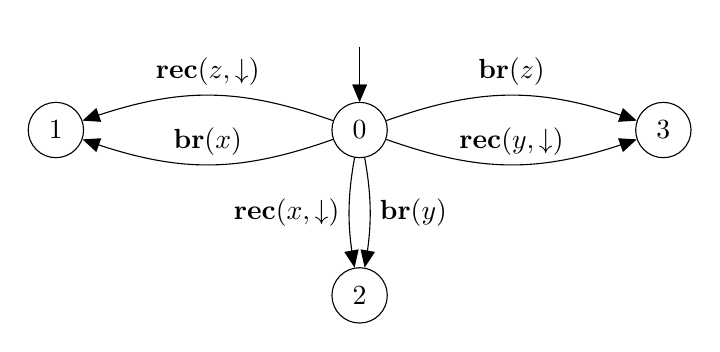
\begin{tikzpicture}[xscale=0.5,AUT style,node distance=2.1cm,auto,>= triangle
	45]
	\tikzstyle{initial}= [initial by arrow,initial text=,initial
	distance=.7cm, initial above]
	%	\tikzstyle{accepting}= [accepting by arrow,accepting text=,accepting
	%	distance=.7cm,accepting where =right]
	
	\node[state,initial, minimum width=0.1pt] (0) at (0,0) {0};
	\node[state] [left of=0, xshift=-50] (x) {1};
	\node[state] [below of=0] (y) {2};
	\node[state] [right of=0, xshift=50] (z) {3};

	\path[->, bend left=10] 	
	(0) edge node[above] {$\brone{x}$} (x)
	(0) edge node {$\brone{z}$} (z)
	;
	\path[->, bend right=10] 	
	(0) edge node[above] {$\recone{y}{\enregact}$} (z)
	(0) edge node[above] {$\recone{z}{\enregact}$} (x)
	;
	\path[->, bend left=20] 	
	(0) edge node {$\brone{y}$} (y)
	;
	\path[->, bend right=20] 	
	(0) edge node[left] {$\recone{x}{\enregact}$} (y)
	;
\end{tikzpicture}
		\caption{An illustrating example}
		\label{fig:no-clique}
	\end{figure}
\end{example}


The rest of this subsection aims to prove that one can only consider "non-contradictory" queries. We formalize this term in the following definition.
\begin{definition}
We say that a "query" $\query$ is ""contradictory"" if either:
	\begin{itemize}
		\item there exists $\varz$ and $q \neq q' \in Q$ such that $\quotemarks{q(\varz)}, \quotemarks{q'(\varz)} \in \query$ or
		
		\item there exist $\var{z_1}, \ldots, \var{z_k} \in \varset$ with $k\geq 1$ such that $\quotemarks{R(\varz_{i}) = R(\varz_{i+1})} \in \query$ for all $i \in \set{1,\ldots,k-1}$ and $\quotemarks{R(\varz_k) \neq R(\varz_1)} \in \query$.
	\end{itemize}
\end{definition}

\begin{proposition}
A "query" $\query$ is "contradictory" if and only if there exists no configuration satisfying $\query$. Additionnaly, one may decide whether $\query$ is contradictory in time polynomial in $\size{\prot} + \size{\query}$. 
\end{proposition}

\ifproofs
\begin{proof}
Suppose first that $\query$ is "contradictory". If there exist $q \ne q'$ such that
 $\quotemarks{q(\varz)}, \quotemarks{q'(\varz)} \in \query$,  then a "configuration" satisfying $\query$ would need to have a single agent in two distinct states. If there exist $\var{z_1}, \ldots, \var{z_k}$ distinct variables with $k>1$ such that $\quotemarks{R(\varz_{i}) = R(\varz_{i+1})} \in \query$ for all $i \in \set{1,\ldots,k-1}$ and $\quotemarks{R(\varz_k) \neq R(\varz_1)} \in \query$, then in any configuration satisfying $\query$, $\varz_k$ and $\varz_1$ must have the same register value but also distinct register values, which is a contradiction. 

Suppose now that the $\query$ is not "contradictory" and show that there exists some configuration satisfying $\query$.

We consider the graph $G$ whose vertices are variables of $\varset$ appearing in $\query$ and with an edge between $\varz$ and $\varz'$ if and only if $R(\varz) = R(\varz') \in \query$. Since $\query$ is not "contradictory", for any $\varz, \varz'$ in the same connected component of $G$, $\quotemarks{R(\varz) \ne R(\varz')} \notin \query$. We construct a configuration satisfying $\query$ with an agent $a_\varz$ for every $\varz$ such that:
\begin{itemize}
\item if $\quotemarks{q(\varz)} \in \query$ then $a_\varz$ is in state $q$,
\item the agents of the variables of a connected component of $G$ have all the same register value.  
\end{itemize}
The built configuration satisfies $\query$, which concludes the proof. 
\end{proof}
\fi

\begin{lemma}
\label{lem:query-decomposition}
Let $\query$ a  "non-contradictory" "query". There exist $K_1, \ldots, K_p \subseteq Q$ with $p \leq \size{\query}$ with the following property: there exists a "run" satisfying $\query$ if and only if for all $i \in \set{1,\ldots, p}$, there is a run satisfying $K_i$. Moreover,such sets $K_1, \dots, K_p$ may be computed in time polynomial in $\size{\prot}$. 
\end{lemma}

\ifproofs
\begin{proof}

	We consider the same graph $G$ as in the previous proof. We decompose $G$ into connected components $C_1, \ldots, C_p$. 
For each $C_i$ we define $K_i = \set{q \in Q \mid \exists \varz \in C_i, q(\varz) \in \query}$. Note that $K_i$ may be empty when there is no constraints on the states of the variables in $C_i$. An empty set is satisfied by any "run". This is coherent with the fact that, when $K_i = \emptyset$, it suffices to assign all variables in $C_i$ to an agent that stays in $q_0$ for the whole "run".

	Suppose there is a "run" satisfying $\query$, let $\config$ be its final configuration, let $\nu$ be a valuation witnessing the satisfaction of $\query$ by $\config$.
	Let $i \in \set{1,\ldots, p}$, we show that $\config$ satisfies $K_i$. For all $\varz \in C_i$, let $(q_\varz,\aval_\varz) = \config(\nu(\varz))$. As $C_i$ is a connected component of $G$ and $\config$ satisfies $\query$, all $\nu(\varz)$ with $\varz \in C_i$ have the same register value, which we call $\aval$. 
	For all $q \in K_i$, there exists $\varz \in C_i$ such that $q(\varz) \in \query$ and thus $q_\varz =q$ and $\aval_\varz =\aval$, thus $C_i$ is satisfied.
	
	For the converse implication, suppose for all $i$ we have a run $\run_i$ over a set of agents $\agents_i$ satisfying $K_i$. We rename agents so that the $\agents_i$ are pairwise disjoint, we introduce fresh agents $a_1, \ldots, a_p$ and we set $\agents = \set{a_1, \ldots, a_p} \sqcup \bigsqcup_{i=1}^p \agents_i$. We consider $\run: \config_0 \step{*} \config$ a "run" in which the sequences of actions of each $\run_i$ are executed sequently by agents from $\agents_i$. In $\run$, agents $a_1$ to $a_p$ are left idle on $q_0$. We build the valuation $\nu$ witnessing that $\run$ satisfies $\query$ as follows. Let $i \in \nset{1}{p}$. If $K_i = \emptyset$ then $\nu$ assigns $a_i$ to every variable of $C_i$. Otherwise, we know that $\config|_{\agents_i}$ satisfies $K_i$ because the final configuration of $\run_i$ does: there exists $\aval_i \in \nats$ such that, for all $q \in K_i$, some agent $a_{i,q}$ has state $q$ and register value $\aval_i$ in $\config$. Let $\varz \in C_i$. If, for some $q \in Q$, $\quotemarks{q(\varz)} \in \query$, $\nu$ assigns agent $a_{i,q}$ to $\varz$ ($q$ is unique as $\query$ is not "contradictory"). If $\query$ has no constraint about the state of $\varz$, $\nu$ assigns to $\varz$ some $a_{i,q}$ with $q \in k_i$ arbitrary. 
	
	% We define a valuation $\nu$ as follows. Let $\varz \in \varset$ and $i$ so that $C_i$ is the connected component of $\varz$ in $G$. If  for some $q$, then this $q$ is unique as $\query$ is not "contradictory". We set $\nu(\varz) = a_q^i$.
	% If there is no $q(\varz)$ for any $q \in Q$ in $\query$ but there is one of the form $q'(\varz')$ with $\varz' \in C_i$, then we set $\nu(\varz) = \nu(\varz')$.
	% Otherwise we set $\nu(\varz) = a_i$.
	% This fully defines our valuation $\nu$.
	
	Clearly all formulas of the form $q(\varz)$ or $R(\varz) = R(\varz')$ are satisfied.
	For the formulas of the form $R(\varz) \neq R(\varz')$, we observe that as $\query$ is not "contradictory", $\varz$ and $\varz'$ are not in the same connected component of $G$. Because the runs $\run_i$ worked with disjoint sets of register values ($\config_0$ is initial), the agents assigned to $\varz$ and $\varz'$ end the run with distinct register values.
	Hence $\data{\config}(\nu(\varz)) \neq \data{\config}(\nu(\varz'))$. As a result, $\query$ is satisfied by $\run$.
\end{proof}
\fi


We are now ready to define our abstraction.

\subsubsection{Abstraction}
\label{sec:abstraction}

The abstraction should keep track of a particular state (the state of the process with the initial register value) and a set of states in which any number of processes can be on with the same non-initial value. We name this tuple a "gang" which we define formally below.

\begin{definition}
	Let $(Q,\transitions, q_0)$ be a protocol.

	A ""gang"" is a pair $\gang = (\boss, \clique) \in (Q \cup \set{\noboss}) \times \powerset{Q}$. The element $\boss$ is the ""boss"" and the set $\clique$ is the ""clique"" of the "gang". %We write $\gangconfigs$ the set of "gangs". 

	Let $\run = \config_0 \step{} \config_1 \step{} \cdots \step{} \config_k$ be a "run" and $\aval \in \valsof{\run}$. The "gang" of value $\aval$ in $\run$, written $\gangof{\aval}{\run}$, is the "gang" $(\boss, \clique)$ such that, 
	\begin{itemize}
	\item if there exists $a_0 \in \agentsof{\run}$ such that, 
	for every 
	$i \in \nset{0}{k}$, 
	$\data{\config_i}(a_0) = \aval$ then $\boss := \st{\config_k}(a_0)$, otherwise $\boss := \noboss$, 
%	\nico{changement de def: pour etre le boss il faut garder sa valeur tt le long de l'execution}
	\item  $\clique := \set{q \in Q \mid \exists i \leq k, \exists a \in \agents\setminus \set{a_0}, \config_i(a) = (q,\aval)}$ %\\
%´\nico{j'ai changé la def pour fque ça soit plus facile: ancienne def $\clique := \set{q \in Q \mid \exists a \in \agents\setminus \set{\boss}, \config_k(a) = (q,\aval)}$}
	\end{itemize}
Note that, if such an agent $a_0$ exists, then it is unique as $\config_0$ is initial hence this definition is sound. If there exists no agents with value $\aval$ in $\config_0$, then trivially $\gangof{\aval}{\run} = (\noboss, \emptyset)$. 
\end{definition} 

Intuitively, a "gang" corresponds to the set of agents with a given "register value". The "boss" $\boss$ represents the process that had this value at the beginning and the "clique" $\clique$ the set of states of processes who have received and stored this register value. If the original owner of this value no longer has it, then $\boss = \noboss$. Note that we define the clique as the set of states $q$ such that \emph{at some point in the run} some agent was in state $q$ with value $v$. This is because we can use the copycat principle to add a large amount of agents that are in state $q$ with value $v$, and thus we can assume that there is always one.

We now define an abstract semantics based on gangs: intuitively, an abstract configuration is composed of a gang along with a set of states which are known to be coverable.

\begin{definition}
\label{def:abstract-configuration}
An ""abstract configuration"" over $\agents$ is a tuple of $2^Q \times \gangset$ where $\gangset$ designates the set of all "gangs". We write $\aconfigs{\agents}$ the set of "abstract configurations" over $\agents$ and $\allaconfigs := \bigcup_{\agents \subseteq \nats \text{ finite }}\aconfigs{\agents}$ the set of all abstract configurations. 

Given two abstract configurations $\aconfig = (\covset, \boss, \clique)$ and $\aconfig' = (\covset', \boss', \clique')$, there is an ""abstract step"" from $\aconfig$ to $\aconfig'$, denoted $\aconfig \step{} \aconfig'$, when $\clique' \subseteq \covset'$, $\boss' \in \covset' \cup \set{\noboss}$ and one of the following cases is satisfied.
\begin{enumerate}
\item \emph{Broadcast from "clique":}
	\begin{enumerate}[i]
		\item\label{item:broadcast_from_clique_broadcast} There exist $\amessage \in \messages$ and $\statebr \in \clique, \statebr' \in \clique'$ s.t. $(\statebr, \brone{m}, \statebr') \in \transitions$. 
		
		\item\label{item:broadcast_from_clique_boss} Either $\boss = \boss'$ or there exists $(\boss, \rec{\amessage}{\anact}, \boss') \in \transitions$ for some action $\anact$.

		\item\label{item:broadcast_from_clique_clique}$(\clique \cup \set{\statebr'}) \subseteq \clique'$ and, for all $q' \in \clique' \setminus (\clique \cup \set{\statebr'})$, there exists $q$ s.t. $(q, \rec{\amessage}{\anact}, q') \in \transitions$ where:
		\begin{itemize}
			\item $\anact = \quotemarks{\eqtestact}$ or $\quotemarks{\dummyact}$ and $q \in \clique$, or
			\item $\anact= \quotemarks{\enregact}$ and $q \in \covset$.
		\end{itemize}
		
		\item\label{item:broadcast_from_clique_covset}$(\covset \cup \set{\statebr'}) \subseteq \covset'$ and, for all $q' \in \covset' \setminus (\covset \cup \set{\statebr'})$, there exists $q$ s.t. $(q, \rec{\amessage}{\anact}, q') \in \transitions$ where:
		\begin{itemize}
			\item  $\anact = \quotemarks{\eqtestact}$ and $q \in \clique$, or
			\item $\anact = \quotemarks{\enregact}$ or $\quotemarks{\dummyact}$ and $q \in \covset$.
		\end{itemize}
	\end{enumerate}


	\item \emph{Broadcast from "boss":}
	\begin{enumerate}[i]
		\item \label{item:broadcast_from_boss_broadcast} there exists $\amessage \in \messages$ such that $(\boss, \brone{m}, \boss') \in \transitions$
		
		\item\label{item:broadcast_from_boss_boss} $\boss, \boss' \ne \noboss$ (technically implied by \ref{item:broadcast_from_boss_broadcast} but written here to match other cases)

		\item\label{item:broadcast_from_boss_clique} 	$\clique \subseteq \clique'$ and, for all $q' \in \clique' \setminus \clique$, there exists $q$ s.t. $(q, \rec{\amessage}{\anact}, q') \in \transitions$ where:
		\begin{itemize}
			\item $\anact = \quotemarks{\eqtestact}$ or $\quotemarks{\dummyact}$ and $q \in \clique$, or
			\item $\anact= \quotemarks{\enregact}$ and $q \in \covset$.
		\end{itemize}
				
		\item\label{item:broadcast_from_boss_covset} $\covset \cup \set{\boss'} \subseteq \covset'$ and, for all $q' \in \covset' \setminus (\covset \cup \set{\boss'})$, there exists $q$ s.t. $(q, \rec{\amessage}{\anact}, q') \in \transitions$ where:
		\begin{itemize}
			\item  $\anact = \quotemarks{\eqtestact}$ and $q \in \clique$, or
			\item $\anact = \quotemarks{\enregact}$ or $\quotemarks{\dummyact}$ and $q \in \covset$.
		\end{itemize}
	\end{enumerate}


	\item \emph{External broadcast:}
	\begin{enumerate}[i]
		\item\label{item:external_broadcast_broadcast} There exists $\amessage \in \messages$ and $\statebr \in \covset, \statebr' \in \covset'$ s.t. $(\statebr, \brone{m}, \statebr') \in \transitions$. 
	
		\item\label{item:external_broadcast_boss}Either $\boss = \boss'$ or:
		\begin{itemize} 
			\item $\boss' \ne \noboss$ and there exists $(\boss, \rec{\amessage}{\dummyact}, \boss') \in \transitions$, or
			\item $\boss' = \noboss$ and there exists $(\boss, \rec{\amessage}{\enregact}, \boss') \in \transitions$.
		\end{itemize}

		\item\label{item:external_broadcast_clique}$\clique \subseteq \clique'$ and, for all $q' \in \clique' \setminus \clique$, there exists $q \in \clique$ s.t. $(q, \rec{\amessage}{\dummyact}, q') \in \transitions$.
		
		\item\label{item:external_broadcast_covset}$(\covset \cup \set{\statebr'}) \subseteq \covset'$ and, for all $q' \in \covset' \setminus (\covset \cup \set{\statebr'})$, there exists $q \in \covset$ s.t. $(q, \rec{\amessage}{\anact}, q') \in \transitions$ where $\anact = \quotemarks{\enregact}$ or $\anact = \quotemarks{\dummyact}$.
	\end{enumerate}
	\item \emph{""Gang reset"":} $S' = S$, $\clique' = \emptyset$ and $\boss'= q_0$
\end{enumerate}


Given a concrete run $\run: \config_0 \step{*} \config_k$, we write \AP  $\intro*\absproj{\aval}{\run}$ for the "abstract configuration" $(\covset, \gangof{\aval}{\run})$ where $\covset$ is the set of all states appearing in $\run$. 

%The set of \emph{initial abstract configurations} is $\aconfiginitset := \set{(\set{q_0}, \boss, \clique)  \mid \boss \in \set{q_0, \noboss}, \clique \subseteq \set{q_0}}$.
The \emph{initial abstract configuration} is $\aconfiginit := (\set{q_0}, q_0, \emptyset)$. 
As in the concrete case, an ""abstract run"" is a sequence $\arun = \aconfig_0, \dots, \aconfig_k$ such that $\aconfig_0 = \aconfiginit$ is the initial configuration and, for all $i$, $\aconfig_i \step{} \aconfig_{i+1}$. We denote such a run $\aconfig_0 \step{*} \aconfig_k$. Similarly, we denote by $\aconfig \step{*} \aconfig'$ the existence of a sequence of steps from $\aconfig$ to $\aconfig'$.
\end{definition}


\begin{lemma}
	\label{lem:short-run}
For every $\aconfig \in \allaconfigs$ such that $\aconfiginit \step{*} \aconfig$, there exists an abstract run $\arun: \aconfig_0 \step{*} \aconfig$ of less that $(|Q|+2)^3$ steps.
% note: this bound is not optimal and is chosen to keep the proof simple
\end{lemma}

\ifproofs
\begin{proof}
Note that $\covset$ may never decrease along an abstract execution and that $\clique$ may only decrease at "gang resets".

We can hence enforce in the abstract semantics that, at least every $|Q|+2$ steps without "reset", either $\covset$ or $\clique$ has increased. Indeed, otherwise the configuration has looped as the boss may only take $|Q| +1$ values. We may also enforce that $\covset$ has strictly increased between two "resets", as otherwise one may remove anything that happened between the two "resets". Therefore, there are at most $|Q|-1$ "gang resets" in total, and each portion of the execution with no "reset" has at most $(|Q|+2)(|Q|+1)$ steps. This yields the bound of the proposition. 
\end{proof}
\fi

We now prove that our abstraction is sound and complete for our problem of interest. 

\subsection{Completeness}
This subsection is devoted to proving Lemma~\ref{lem:abstraction_complete}.

\begin{lemma}
\label{lem:abstraction_complete}
If $\run$ is a (concrete) "run" and $\aval \in \valsof{\run}$, then $\aconfiginit \step{*} \absproj{\aval}{\run}$. 
\end{lemma}


% The following lemma shall later be useful:
% \begin{lemma}
% \label{lem:adding_states_in_covset}
% If $\aconfig = (\covset, \gang), \aconfig' = (\covset', \gang') \in \allaconfigs$ are such that $\aconfig \step{*} \aconfig'$ then $\covset \subseteq \covset'$ and, for all $T \subseteq Q$, $(\covset \cup T, \gang) \step{*} (\covset' \cup T, \gang')$. 
% \end{lemma}
% \begin{proof}
% To prove the first statement, in suffices to observe that, in a step of the abstract semantics, the set $\covset$ may not decrease.
% To prove the second statement, it suffices to notice in the abstract semantics that a larger $\covset$ may never hinder a step. 
% \end{proof}

\begin{lemma}
\label{lem:proof_completeness_covset_constant}
For all "runs" $\run: \config_0 \step{*} \config$ and $\aval \in \valsof{\run}$, $(\statesin{\run}, q_0, \emptyset) \step{*} \absproj{\aval}{\run}$. 
\end{lemma}

\ifproofs
\begin{proof}
Let $\covset := \statesin{\run}$ and $\agents = \agentsof{\run}$.

Thanks to Remark~\ref{rem:run_no_new_register_values},  $\aval$ appears in $\config_0$; let $a_0$ be the (unique) agent such that $\data{\config_0}(a_0) = \aval$. We write $\run : \config_0 \step{} \config_1 \step{} \dots \step{} \config_k = \config$. For every $i \leq k$, let $\run_i : \config_0 \step{*} \config_i$ be the prefix of $\run$ of length $i$, and write $\aconfig^i := (\covset, \gangof{\aval}{\run_i})$. Note that $\gangof{\aval}{\run_0} = (q_0, \emptyset)$ hence $\aconfig^0 = (\covset, q_0, \emptyset)$. Also, we write $(\covset, \boss_i, \clique_i) := \aconfig^i$.

We prove by induction on $i$ that $\aconfig^0 \step{*} \aconfig^i$.
The statement is trivially true for $i =0$. 

Suppose now that $(\covset, \emptyset, \noboss) \step{*} \aconfig^i$. 
If suffices to prove that $\aconfig^i \step{} \aconfig^{i+1}$. First of all we clearly have, by definition, $K_{i+1} \subseteq S$ and $\boss_{i+1}\in S\cup\set{\noboss}$. We consider the last step of $\run_{i+1}$, which is referred to under the name $s_{i+1}$ in what follows; $s_{i+1}: \config_i \step{} \config_{i+1}$. Let $\agentbr$ the agent making the broadcast transition in $s_{i+1}$ and $A_{\recsymb}$ the set of agents receiving this broadcast in $s_{i+1}$. Let $(\statebr, \brone{\amessage}, \statebr') \in \transitions$ denote the transition taken by $\agentbr$ in $s_{i+1}$.

We now make the following case distinction to determine the type of the abstract step $\aconfig^i \step{} \aconfig^{i+1}$:
\begin{enumerate}
\item\label{proof_completeness:case_broadcast_clique} if $\data{\config_{i}}(\agentbr) = \aval$ but there exists $j<i$ such that $\data{\config_{j}}(\agentbr) \ne \aval$ then it is a ``broadcast from clique'',
\item\label{proof_completeness:case_broadcast_boss} if, for all $j \leq i$, $\data{\config_j}(\agentbr) = \aval$ then it is a ``broadcast from boss'',
\item\label{proof_completeness:case_external_broadcast} otherwise it is an ``external broadcast''. 
\end{enumerate}
Note that $\agentbr$ may not change its register value in $s_{i+1}$ hence $\data{\config_i}(\agentbr) = \data{\config_{i+1}}(\agentbr)$. 

Let $\agentboss$ the agent such that $\data{\config_0}(\agentboss) = \aval$. In case~\ref{proof_completeness:case_broadcast_boss}, $\agentboss = \agentbr$; in the other two cases, $\agentboss \ne \agentbr$. 

We now prove the other conditions:
\begin{enumerate}[i]
\item In case~\ref{proof_completeness:case_broadcast_clique}, since $\agentbr$ has value $\aval$ in $\config_i$ and $\config_{i+1}$ but not in every $\config_j$ for $j \leq i$, we directly have $\statebr \in \clique_i$ and $\statebr' \in \clique_{i+1}$. In case~\ref{proof_completeness:case_broadcast_boss}, it suffices to note that $\boss_i = \st{\config}(\agentbr)$ and $\boss_{i+1} = \st{\config_{i+1}}(\agentbr)$. In case~\ref{proof_completeness:case_external_broadcast}, it suffices to note that $\statebr, \statebr' \in \covset$ as both states appear in $\run$.
\item In case~\ref{proof_completeness:case_broadcast_boss}, this condition is automatically satisfied. In the other two cases, we look at what $\agentboss$ does in $s_{i+1}$. If it remains idle then we have $\boss_i = \boss_{i+1}$. Otherwise it takes a reception transition as $\agentbr \ne \agentboss$. 
In case~\ref{proof_completeness:case_external_broadcast}, this reception may not have action $\quotemarks{\eqtestact}$ as the broadcast is from an agent with register value that is not $\aval$ ($\data{\config_i}(\agentbr) \ne \aval$ by hypothesis). For the same reason, if this reception has action $\quotemarks{\enregact}$ then $\boss_{i+1}= \noboss$. If this reception has action $\quotemarks{\dummyact}$ and $\boss_i \ne \noboss$ then $\boss_{i+1} \ne \noboss$ as $\agentboss$ keeps value $\aval$.
\item We have $\clique_i \subseteq \clique_{i+1}$ because $\run_{i}$ is a prefix of $\run_{i+1}$; also, in case~\ref{proof_completeness:case_broadcast_clique}, $\statebr' \in \clique_{i+1}$ because of $\agentbr$. Let $q' \in \clique_{i+1} \setminus \clique_i$ with, in case~\ref{proof_completeness:case_broadcast_clique}, $q' \ne \statebr'$. There exist $q\in \covset$ and an agent $a$ that takes a reception transition $(q, \rec{\amessage}{\anact}, q')$ in $s_{i+1}$ and has value $\aval$ in $\config_{i+1}$. In cases~\ref{proof_completeness:case_broadcast_clique} and \ref{proof_completeness:case_broadcast_boss}, the broadcast has value $\aval$ hence if $\anact = \quotemarks{\eqtestact}$ or $\quotemarks{\dummyact}$ then $a$ has value $\aval$ in $\config_i$ and $q \in \clique_i$. In case~\ref{proof_completeness:case_external_broadcast}, the broadcast has value $\ne \aval$ hence $a$ may have value $\aval$ in $\config_{i+1}$ only when $\anact = \quotemarks{\dummyact}$ and $a$ had value $\aval$ in $\config_i$, which implies $q \in \clique_i$. 
\item It suffices to note that the first components of $\aconfig^i$ and $\aconfig^{i+1}$ are equal to $\covset$ and $\statebr' \in \covset$, and $\boss_{i+1} \in \covset \cup \set{\bot}$. 
\end{enumerate}
 
Overall, we have proven that $\aconfig^i \step{} \aconfig^{i+1}$, which concludes the induction step. Appyling the result with $i = k$ proves Lemma~\ref{lem:proof_completeness_covset_constant}. 

\end{proof}
\fi

\ifproofs
We may now prove Lemma~\ref{lem:abstraction_complete}. 

\begin{proof}[Proof of Lemma~\ref{lem:abstraction_complete}]
Let $\run$ a run.
We proceed by induction on the size of the set $\statesin{\run}$. 
First, if $\statesin{\run}$ is of size $1$ then $\statesin{\run} = \set{q_0}$. Applying Lemma~\ref{lem:proof_completeness_covset_constant} directly gives $\aconfiginit = (\set{q_0}, q_0, \noboss) \step{*} \absproj{\aval}{\run}$.


Suppose now that the statement is true for any $\run$ such that $\statesin{\run}$ is of size $k$, and suppose that we have a run $\run$ such that $\statesin{\run}$ is of size $k+1$. Let $\aval \in \valsof{\run}$. Let $\run_p: \config_0 \step{*}\config_p$ the longest suffix of $\run$ such that $\statesin{\run} \ne \statesin{\run_p}$. By induction hypothesis, we know that for all $\aval \in \valsof{\run}$, $\aconfiginit \step{*} \absproj{\aval}{\run_p}$. Write $s$ the step immediatly after $\run_p$ in $\run$. By maximality of $\run_p$, $\run_p s$ covers all states in $\statesin{\run} \setminus \statesin{\run_p}$. 

Write $\agentbr$ the agent broadcasting in $s$, $(\statebr, \brone{\amessage}, \statebr')$ the corresponding transition and $\avalbr$ the broadcast value. By induction hypothesis applied to $\run_p$ and $\avalbr$, $\aconfiginit \step{*} \absproj{\avalbr}{\run_p}$. Applying Lemma~\ref{lem:proof_completeness_covset_constant} on $\run$ and $\aval$ gives that $(\statesin{\run}, q_0, \emptyset) \step{*} \absproj{\aval}{\run}$. Therefore, it remains to prove that $\absproj{\aval}{\run_p} \step{*} (\statesin{\run}, q_0, \emptyset)$. It suffices to prove that there exists $\boss, \clique$ such that $\absproj{\avalbr}{\run_p} \step{} (\statesin{\run}, \boss,\clique)$, a "gang reset" allowing us to then reach $(\statesin{\run}, q_0, \emptyset)$. In other words, we prove that, from $\absproj{\avalbr}{\run_p}$, one may cover all states in $\statesin{\run}$ in just one abstract step.

We aim at proving that $\absproj{\avalbr}{\run_p} \step{} (\statesin{\run}, \boss,\clique)$ for well-chosen $\boss$ and $\clique$.
Just like in the proof of Lemma~\ref{lem:proof_completeness_covset_constant}, we make a case disjunction to prove that the broadcast in $s$ may be mimicked in the abstraction from $\absproj{\avalbr}{\run_p}$. The type obtained is either a "broadcast from clique" or a "broadcast from boss", because by hypothesis the agent broadcasting has value $\avalbr$ and therefore its state before the broadcast is either the boss or in the clique in $\absproj{\avalbr}{\run_p}$. 

Because we may choose $\boss$ and $\clique$ freely, the only challenging condition is \ref{item:broadcast_from_clique_covset}.
Let $q' \in \statesin{\run} \setminus \statesin{\run_p}$, $q' \ne \statebr'$. 
There exists an agent $a$ that takes a reception transition $(q,\rec{m}{\anact},q')$ in $s$. 
If $\anact = \quotemarks{\eqtestact}$, then agent $a$ has value $\avalbr$ at the end of $\run_p$ hence $q$ is in the clique of $\absproj{\avalbr}{\run_p}$ and condition \ref{item:broadcast_from_clique_covset} is satisfied. Otherwise, one has $q \in \statesin{\run_p}$ and condition \ref{item:broadcast_from_clique_covset} is satisfied.
In the end, there exist $\boss$, $\clique$ such that $\absproj{\avalbr}{\run_p} \step{} (\statesin{\run}, \boss,\clique)$. By a "gang reset", this implies that $\absproj{\avalbr}{\run_p} \step{*} (\statesin{\run}, q_0, \emptyset)$; we have proven that $\aconfiginit \step{*}\absproj{\avalbr}{\run_p} \step{*} (\statesin{\run}, q_0, \emptyset) \step{*} \absproj{\aval}{\run}$ which concludes the proof. 
\end{proof}
\fi

\subsection{Soundness}
\label{sec:soundness}

%\begin{lemma}[Strong copycat]\label{lem:strong-copycat}
%	Let $q \in Q$ and  $\run : \config_0 \step{*} \config_f$ an "initial run"  that covers $q$. Write $\agents := \agentsof{\run}$. There exists $\agents' \subseteq \nats$ finite, a bijection $\psi : \agents \to \agents'$ and a "run" $\run': \config_0' \step{*} \config_f'$ over $\agents \cup \agents'$ such that:
%	\begin{itemize}
%		\item for all $a \in \agents$, $\config_f'(a) = \config_f(a)$ (agents of $\agents$ behave the same in $\run$ and $\run'$),
%		\item for all $a' \in \agents'$, $\st{\config_f'}(a') = \st{\config_f}(\psi^{-1}(a'))$,
%		\item for all $a \in \agents$, either $\data{\config_f}(a) = \data{\config_0}(a)$ and $\data{\config_f'}(a') = \data{\config_0'}(a')$ or $\data{\config_f'}(\psi(a)) = \data{\config_f'}(a)$.
%	\end{itemize}
%\end{lemma}
%
%\begin{proof}
%	Let $\agents' \subseteq \nats$ such that $|\agents'|= |\agents|$ and $\agents \cap \agents' = \emptyset$. 
%	There exists a bijection $\psi: \agents \mapsto \agents'$. Let $M = 1+ \max\set{\data{\config_0}(a) \mid a \in \agents}$.
%	Let $\config_0'$ an initial configuration over $\agents \cup \agents'$ which is equal to $\config_0$ on every agent of $\agents$, and such that $\config'_0(\psi(a)) = \config_0(a) +M$ for all $a \in \agents$. 
%	The constructed "run" $\run'$ over $\agents \cup \agents'$ starts on configuration $\config_0'$. We define it by induction on $\run$.
%	
%	Let $\run = \config_0 \to \config_1 \to \cdots \to \config_n$, let $u = \config_1 \to \cdots \to \config_{n-1}$, suppose we have a run $u' = \config_0' \to \cdots \to \config_{k}'$ over $\agents \cup \agents'$ such that $u$ and $u'$ satisfy the conditions of the lemma.
%	
%	Let $a$ be the broadcasting agent in the last step of $\run$, $m$ the corresponding message.
%	We have $\config_{n-1}(a) = \config_{k}'(a)$.
%	
%	First, we extend $u'$ by making $\psi(a)$ broadcast $m$, and no agent receives it.
%	We obtain a configuration $\config'_{k+1}$, which is equal to $\config'_k$ except that $\psi(a)$ is now in state $\st{\config_{n}}(a)$.
%	
%	Second we make $a$ broadcast $m$ and for all $a_r \in \agents$ that receives the message in $\config_{n-1} \to \config_n$ with an operation $\alpha$, we make both $a_r$ and $\psi(a_r)$ receive it with the same operation.
%	We have to show that this is a correct transition for all $a_r$.
%	
%	\paragraph{First case: $\config_{n-1}(a_r) \neq \config'_{k}(\psi(a_r))$}  Then $a_r$ and $\psi(a_r)$ both still have their initial value, hence the action $\alpha$ cannot be an equality test
%	
%	
%	First we make $a$ broadcast the same message, and 
%	
%	$\psi(a)$ moves in $\run'$ instead, and if the broadcasting agent has register value $v$ in $\run$ then it has value $v+M$ in $\run'$. In this second part, agents of $\agents$ are left idle. Write $\config_f'$ the final configuration of $\run'$. Since agents of $\agents$ behave the same in $\run$ and $\run'$, for all $a \in \agents$, $\config_f(a) = \config_f'(a')$.
%	A straightforward induction shows that this is indeed a correct run, and that in the end of $\run'$ the states and values of agents of $\agents$ are the same as at the end of $\run$, and that for all $a \in \agents$ we have $\config_f'(\psi(a)) = (\st{\config_f}(a), \data{\config_f}(a) +M)$.
%	
%	From this we immediately infer the conditions of the lemma.
%\end{proof}


\begin{lemma}
	\label{lem:correctness-construction}
	
	\luin{donner de l'intuition sur lemma 39}
	Let $\sigma_0 \in \aconfiginitset$, and $\sigma_0 \to \sigma_1 \to \cdots \to \sigma_n$ an abstract run. For all $i$ let $(S_i, b_i, K_i) := \sigma_i$. Let $M = \size{\Delta}+1$.
	
	For all $i$, there exist a set of agents $\agents_i$, a configuration $\config_i$, a run $\run_i : \config_0 \step{*} \config_i$ over $\agents_i$, agents $a_0, \cdots, a_n \in \agents_i$ and values $v_0, \ldots, v_n \in \nats$ such that:
	\begin{itemize}
		\item for all $s \in S_i$, there are at least $M^{n-i}$ agents (different from $a_i$) in state $s$ 
		
		\item for all $s \in K_i$, there are at least $M^{n-i}$ agents (different from $a_i$) in state $s$ with value $v_i$
		
		\item if $b_i \neq \noboss$, then $a_i$ is in state $b_i$ with value $v_i$.
	\end{itemize}
\end{lemma}

\ifproofs
\begin{proof}

We proceed by induction on $i$.
We set $\agents_0 = \set{1, \ldots, M^n}$, and we set $\config_0(a) = (q_0, a)$ for all $a$. Clearly $\config_0$ satisfies the requirements with respect to $\sigma_0$, with $a_0 = v_0 \in \agents$.

Now assume we constructed $\config_0 \step{*} \cdots \step{*} \config_{i}$ over $\agents_i$ satisfying the conditions of the lemma, we construct $\config_{i+1}$ using a case distinction on the form of the transition $\sigma_i \to \sigma_{i+1}$.
For each $s \in S\setminus K$ we define $\agents_{i,s}$ as the set of agents in state $s$ in $\config_{i}$. We have $\size{\agents_{i,s}} \geq M^{n-i}$ thus we can extract $M = \size{\Delta}+1$ disjoint sets of agents $(\agents_{i,s}^d)_{d \in \Delta\cup\set{\epsilon}}$ from it.
Similarly, for each $s \in K$ we define $\agents_{i,s}$ as the set of agents in state $s$ \textbf{with value $\mathbf{v_i}$} in $\config_{i}$. We have $\size{\agents_{i,s}} \geq \size{\Delta}^{n-i}$ thus we can extract $\size{\Delta}+1$ disjoint sets of agents $(\agents_{i,s}^d)_{d \in \Delta\cup\set{\epsilon}}$ from it.
\\

\textbf{Case 1: } If $\sigma_i \to \sigma_{i+1}$ is a \emph{broadcast from the clique} $d = (q, \brone{m}, q')$ with $q \in K_i$, then we make all agents $a \in \agents_{i,q}^{d}$ (which all have value $v_i$) execute that transition one by one.
None of those broadcasts are received by any other agent, except for the last one:
If $b \neq b'$ then there is a transition $(b, \rec{m}{\alpha}, b')$ and we make $a_i$ execute it upon receiving the broadcast. We then set $a_{i+1} = a_i$.
For all $k' \in K_{i+1} \setminus K_i$ there exists a transition $d'=(k, \rec{m}{\alpha}, k')$ such that either $\alpha$ is $\eqtestact$ or $*$ and $k \in K_i$ or $\alpha$ is $\enregact$ and $k\in S$.
In both cases we make all agents of $\agents_{i,k}^{d'}$ take that transition.

For all $s' \in S_{i+1} \setminus (S_i \cup K_{i+1})$ there exists a transition $d'=(s,\rec{m}{*},s')$ (the operation cannot be $\enregact$ or $\eqtestact$ as otherwise $s$ would be in $K_{i+1}$). We then make all agents of $\agents_{i,s}^{d'}$ follow that transition. 

We set $v_{i+1} = v_i$.
\\

\textbf{Case 2: }If $\sigma_i \to \sigma_{i+1}$ is a \emph{broadcast from the boss} $d = (b_i, \brone{m}, b_{i+1})$, then we make $a_i$ (which has value $v_i$) execute that transition, and we set $a_{i+1} = a_i$.
The agents receiving that message are as follows:

For all $k' \in K_{i+1} \setminus K_i $ there exists a transition $d'=(k, \rec{m}{\alpha}, k')$ such that $\alpha$ is either $\eqtestact$ or $*$ and $k \in K_i$ or $\alpha$ is $\enregact$ and $k\in S$.
In both cases we make all agents of $\agents_k^{d'}$ take that transition.

For all $s' \in S_{i+1} \setminus (S_i \cup K_{i+1} \cup \set{b_{i+1}})$ there exists a transition $d'=(s,\rec{m}{*},s')$ (the operation cannot be $\enregact$ or $\eqtestact$ as otherwise $s$ would be in $K_{i+1}$). We then make all agents of $\agents_s^{d'}$ follow that transition. 

By definition of an "abstract run", we must have $b_i \in S_i$.
Hence we can make all agents of $\agents_{i,s}^{d}$ execute $d$, with no agent receiving the corresponding broadcasts.

We set $v_{i+1} = v_i$.
\\

\textbf{Case 3: } If $\sigma_i \to \sigma_{i+1}$ is an \emph{external broadcast} $d = (q, \brone{m}, q')$ , then we make all agents $a \in \agents_q^{d}$ execute that transition one by one. None of those broadcasts are received by any other agent, except for the last one:
If $b_i \neq b_{i+1}$ then there is a transition $(b, \rec{m}{\alpha}, b'')$ and either $b_{i+1} = b'' \neq \noboss$ and $\alpha = *$ or $b_{i+1} = \noboss$ and $\alpha=\enregact$. In both cases we make $a_i$ execute that transition, and we set $a_{i+1} = a_i$.

For all $k' \in K_{i+1} \setminus K_i$ there exists a transition $d'=(k, \rec{m}{*}, k')$ with $k \in K_i$. We make all agents of $\agents_k^{d'}$ take that transition.

For all $s' \in S_{i+1} \setminus (S_i \cup K_{i+1})$ there exists a transition $d'=(s,\rec{m}{\alpha},s')$ with $\alpha \in \set{*, \enregact}$. We then make all agents of $\agents_s^{d'}$ follow that transition. 

We set $v_{i+1} = v_i$.
\\

\textbf{Case 4: }  If $\sigma_i \to \sigma_{i+1}$ is a \emph{gang reset} then no agent moves and we select some $a_{i+1}$ in $\agents_{q_0}$ and set $v_{i+1}$ to be its value.
\\
%\paragraph{In all cases:} After applying the given transitions, we use the copycat property: we add to $\agents_i$ $M^{n-i-1}$ disjoint copies of itself to obtain $\agents_{i+1}$, and repeat the run constructed thus far over each copy separately. This is to ensure that there are $M^{n-i-1}$ agents in $b_{i+1}$ (if it is not $\noboss$) after this step.

Throughout the case distinction we have ensured that:
\begin{itemize}
	\item If $b_{i+1} \neq \noboss$ then $a_{i+1}$ is an agent of value $v_{i+1}$.
	
	\item For all $k \in K_{i}$, the agents of $\agents_{i,k}^\epsilon$ do not move between configurations $\config_{i}$ and $\config_{i+1}$, hence they have state $k$ and value $v_{i+1}$ in $\config_{i+1}$.
	
	\item If the step is not a gang reset, then $v_{i+1} = v_i$ and for all $k' \in K_{i+1} \setminus K_i$, there exists $d \in \Delta$ from some $k$ to $k'$ such that all agents of $\agents_{i,k}^d$ take that transition. Furthermore, if $d$ is of the form $(k,\rec{m}{\enregact},k')$ then the broadcasting process has value $v_i$, thus all those agents keep value $v_i = v_{i+1}$. 
%	As $\size{\agents_{i,k}^d}\geq M^{n-i-1}$, there are at least that many agents with value $v_{i+1} = v_i$ in $k'$.
	
	\item For all $s \in S_{i}$, the agents of $\agents_{i,s}^\epsilon$ do not move between configurations $\config_{i}$ and $\config_{i+1}$, hence they have state $s$ in $\config_{i+1}$.
	
	\item If the step is not a gang reset, for all $s' \in S_{i+1} \setminus (S_i \cup \set{b_{i+1}})$, there exists $d \in \Delta$ from some $s \in S_i$ to $s'$ such that all agents of $\agents_{i,s}^d$ take that transition.
	
	\item If the step is a gang reset, the conditions of the lemma hold trivially.
\end{itemize}

As a result, we have ensured that the conditions of the lemma were respected.
This concludes our induction.
\end{proof}
\fi

\begin{corollary}
	\label{cor:soundness}
%	For all $\sigma_0 \in \aconfiginitset$ and $\sigma = (S, b, K) \in \Sigma$ such that $\sigma_0 \step{*} \sigma$ there exists a reachable configuration $\gamma$ 
%	satisfying $K \cup \set{b}$ if $b \neq \noboss$ and $K$ otherwise.
	For all $\sigma_0 \in \aconfiginitset$ and $\sigma = (S, b, K) \in \Sigma$ such that $\sigma_0 \step{*} \sigma$, for all $s \in S$, there exists a reachable configuration $\gamma$ covering $s$.
%	satisfying $K \cup \set{b}$ if $b \neq \noboss$ and $K$ otherwise.
\end{corollary}

\ifproofs
\begin{proof}
	We simply apply Lemma~\ref{lem:correctness-construction} to an "abstract run" $\sigma_0 \to \cdots \sigma_n = \sigma$ from $\sigma_0$ to $\sigma$ by setting $i = n$.
%	We obtain (by setting $i = n$) that there exists a value $v_n$ in the final configuration of the constructed run, for all $s \in K$, there is an agent with value $v_n$ in state $s$. Furthermore, if $b \neq \noboss$, then there is an agent in state $b$ with value $v_n$.  
\end{proof}
\fi


\section{An \np algorithm}

\begin{proposition}
	\label{prop:sound-and-complete}
	Let $K$ be a set of states, there exists a reachable "configuration" satisfying $K$ if and only if there exists a reachable "abstract configuration" $(S,b,K')$ with either $K \subseteq K'$ or $b \neq \noboss$ and $K \subseteq K' \cup \set{b}$.  
\end{proposition}

\begin{proof}
	The right-to-left direction is given by Corollary~\ref{cor:soundness}.
	
	For the left-to-right direction, let $\run$ be a run ending in a configuration $\config$ satisfying $K$. Let $v \in \nats$ be such that $\config$ has some agents with value $v$ in every state of $K$.
	
	We construct a suitable "abstract run" as follows: by Lemma~\ref{lem:abstraction_complete} there exists an abstract run from some $\sigma_0 \in \aconfiginitset$ to an abstract configuration $\absproj{v}{\run} = (S, b, K')$.
	
	As $\config, v$ satisfies $K$, for all $s \in K$ either $s = b$ or $s \neq b$ and there exists an agent with state $s$ and value $v$ in $\config$. 	
	By definition of the abstraction $\absproj{v}{\run}$, we have $K \subseteq K'$ if $b=\noboss$ and $K \subseteq K' \cup \set{b}$ otherwise, proving the proposition.
\end{proof}

\begin{theorem}
	\label{thm:np-complete-query-cover}
	The "query coverability problem" is \np-complete.
\end{theorem}

\begin{proof}
	The lower bound is given by Proposition~\ref{prop:np-hard-query-cover}.
	For the upper bound, say we are given a "protocol" $\prot = (Q, \messages, \Delta, q_0)$ and a "query" $\phi$.
	We start by decomposing $\phi$ into cliques $K_1, \ldots, K_p$ in polynomial time, as in Lemma~\ref{lem:query-decomposition}.
	For each $i$, we have to verify that there exists a reachable configuration $\config_i$ satisfying $K_i$. By Proposition~\ref{prop:sound-and-complete}, it is the case if and only if there is an "abstract run" to an "abstract configuration" $(S,b, K)$ with either $K_i \subseteq K$ or $b\neq \noboss$ and $K_i \subseteq K\cup\set{b}$.
	Furthermore, by Lemma~\ref{lem:short-run} if there is such an "abstract run" then there is one with at most $(\size{Q}+2)^3$ steps. 
	Thus we can simply guess such an abstract run and verify it in polynomial time.
	As a result, the "query coverability problem" is in \np. 
\end{proof}
%	
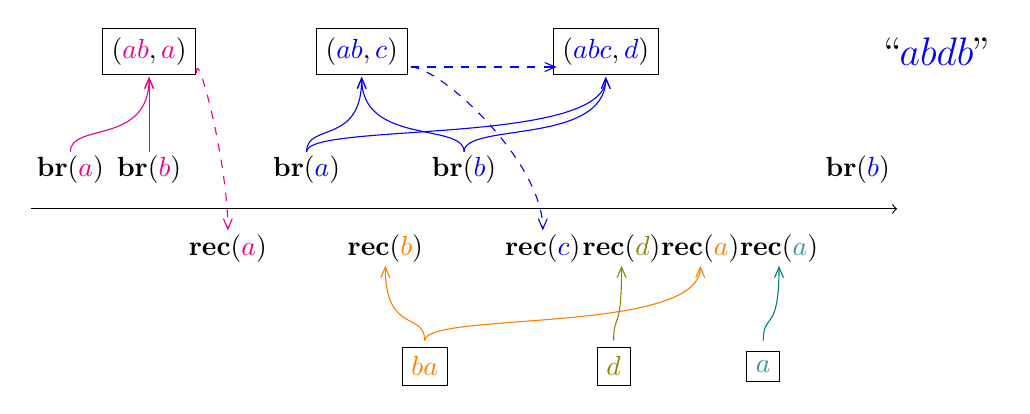
\begin{tikzpicture}
	
	\draw[->, ] (-0.5,0) -- (10.5,0);
	
	\node (b) at (0,0.5) {$\brone{\color{magenta}a\color{black}}$};
	\node (b) at (1,0.5) {$\brone{\color{magenta}b\color{black}}$};
	\node (b) at (3,0.5) {$\brone{\color{blue}a\color{black}}$};
	\node (b) at (5,0.5) {$\brone{\color{blue}b\color{black}}$};
	\node (b) at (10,0.5) {$\brone{\color{blue}b\color{black}}$};
	
	\node (b1) at (0,0.6) {};
	\node (b2) at (1,0.6) {};
	\node (b3) at (3,0.6) {};
	\node (b4) at (5,0.6) {};
	\node (b5) at (10,0.6) {};
	
	\node (sp) at (11,2) {\Large ``$\color{blue}abdb\color{black}$''};
	
	
	\node (r) at (2,-0.5) {$\recsymb(\color{magenta}a\color{black})$};
	\node (r) at (4,-0.5) {$\recsymb(\color{orange}b\color{black})$};
	\node (r) at (6,-0.5) {$\recsymb(\color{blue}c\color{black})$};
	\node (r) at (7,-0.5) {$\recsymb(\color{olive}d\color{black})$};
	\node (r) at (8,-0.5) {$\recsymb(\color{orange}a\color{black})$};
	\node (r) at (9,-0.5) {$\recsymb(\color{teal!80}a\color{black})$};
	
	 \node (r1) at (2,-0.4) {};
	 \node (r2) at (4,-0.6) {};
	 \node (r3) at (6,-0.4) {};
	 \node (r4) at (7,-0.6) {};
	 \node (r5) at (8,-0.6) {};
	 \node (r6) at (9,-0.6) {};
	
	\node[draw] (f1) at (1,2) {$(\color{magenta}ab\color{black}, \color{magenta}a\color{black})$};
	\node[draw] (f2) at (3.7,2) {$(\color{blue}ab\color{black}, \color{blue}c\color{black})$};
	\node[draw] (f3) at (6.8,2) {$(\color{blue}abc\color{black}, \color{blue}d\color{black})$};
	\node (fa1) at (1,1.8) {};
	\node (fa'1) at (1.6,1.6) {};
	\node (fa2) at (3.7,1.8) {};
	\node (fa'2) at (4.2,1.8) {};
	\node (fa3) at (6.8,1.8) {};
	\node (fa'3) at (6.3,1.8) {};
	
	
	\node[draw] (bo1) at (4.5,-2) {$\color{orange}ba\color{black}$};
	\node[draw] (bo2) at (6.9,-2) {$\color{olive}d\color{black}$};
	\node[draw] (bo3) at (8.8,-2) {$\color{teal!80}a\color{black}$};
	
	
	\node (ba1) at (4.5,-1.8) {};
	\node (ba2) at (6.9,-1.8) {};
	\node (ba3) at (8.8,-1.8) {};
	
	\draw[color=magenta, ->, >=angle 45] (b1) ..controls +(0,0.5) and +(0,-1).. (fa1);
	\draw[color=magenta, ->, >=angle 45] (b2) ..controls +(0,0.5) and +(0,-1).. (fa1);
	
	\draw[color=blue, ->, >=angle 45] (b3) ..controls +(0,0.5) and +(0,-1).. (fa2);
	\draw[color=blue, ->, >=angle 45] (b4) ..controls +(0,0.5) and +(0,-1).. (fa2);
	
	\draw[color=blue, ->, >=angle 45] (b3) ..controls +(0,0.5) and +(0,-1).. (fa3);
	\draw[color=blue, ->, >=angle 45] (b4) ..controls +(0,0.5) and +(0,-1).. (fa3);
	
	\draw[color=orange, ->, >=angle 45] (ba1) ..controls +(0,0.5) and +(0,-1).. (r2);
	\draw[color=orange, ->, >=angle 45] (ba1) ..controls +(0,0.5) and +(0,-1).. (r5);
	
	\draw[color=olive, ->, >=angle 45] (ba2) ..controls +(0,0.5) and +(0,-1).. (r4);
	\draw[color=teal, ->, >=angle 45] (ba3) ..controls +(0,0.5) and +(0,-1).. (r6);
	
	\draw[color=magenta, ->, >=angle 45, dashed] (fa'1) ..controls +(0,0.5) and +(0,1).. (r1);
	\draw[color=blue, ->, >=angle 45, dashed] (fa'2) ..controls +(0.5,0) and +(0,1).. (r3);
	\draw[color=blue, ->, >=angle 45, dashed] (fa'2) ..controls +(0.5,0) and +(-0.5,0).. (fa'3);
\end{tikzpicture}


	\section{Conclusion}
	\luin{parler target r = 1, pile, enrichir les tests possibles}
	
	\bibliography{biblio}
	
	\newpage
	
	\appendix
%	\section{Proof of Proposition~\ref{prop:reduction-LCS}}
\label{app:reduction-lcs}

\propReductionLCS*

\begin{proof}
	It is sufficient to prove that it is as hard as reachability for lossy channel systems with a single channel, which corresponds to a single finite-state machine that has the ability to buffer symbols in a lossy FIFO queue \cite{Schnoebelen2002verifying}. We present here a polynomial-time reduction.
	Let $\los := (\lstates,\Sigma)$ be a "lossy channel system", where $\lstates$ is a finite set of locations, $\Sigma$ is a finite set of symbols and $\ltransitions \subseteq \lstates \times \Sigma^* \times \set{!, ?} \times \lstates$; $\quotemarks{!}$ corresponds to a "push" (writing at the end of the channel) and $\quotemarks{?}$ to a "pop" (reading at the beginning the channel). A configuration of $\los$ is a pair of $\lstates \times \Sigma^*$ denoting the location of the system and the content of the channel. There exists a step from $(\lstate,w)$ to $(\lstate',w')$ using transition $\ltrans \in \ltransitions$, denoted $(\lstate,w) \lstep{\ltrans} (\lstate',w')$, when
	\begin{itemize}
		\item $\ltrans = (\lstate,u,!,\lstate')$ for some $u \in \Sigma^*$ and $w' \subword w \cdot u$ (a ""push""),
		\item $\ltrans = (\lstate,u,?,\lstate')$ for some $u \in \Sigma^*$ and $u \cdot w' \subword w$ (a ""pop"")
	\end{itemize}
	where $\subword$ denotes the "subword" order.
	This subword order encodes the lossiness of the channel (a non-lossy channel would have equalities instead); intuitively, it expresses the fact that letters in the channel may get lost. 
	
	The existence of such a transition for some $\ltrans \in \transitions$ is denoted $(\lstate,w) \lstep{} (\lstate',w')$, and its transitive closure is denoted $\lstep{*}$. The ""reachability problem@@lcs"" asks, given $\los$ and two locations $\lstate_i, \lstate_f \in \lstates$, whether there exists an execution $(\lstate_i,\epsilon) \lstep{*} (\lstate_f, w)$ for some $w$. 
	
	We aim at constructing a protocol $\prot$ with two registers with a distinguished state $q_f$ such that $q_f$ may be covered if and only if $(\los, q_i, q_f)$ is a positive instance of the "reachability problem@@lcs". 
	The intuition of $\prot$ is the following. Agents will organize in chains so that each agent of a chain knows the identifier of its predecessor in the chain, hence is able to check that messages received come from it. Each agent of the chain is meant to encode a step of the execution in the "lossy channel system". 
	An agent of the chain will only listen to their predecessor in the chain, from which they will obtain a location of the system and the content of the channel. As it receives those, it will broadcast the new location of the system and the new content of the channel to the next agent of the chain. 
	
	Note that the content of the channel might become big in a "lossy channel system", therefore agents will not store it but rather rebroadcast it letter by letter. An agent only applies a small modification at the beginning of the channel if it decides to encode a "pop" transition and at the end of the channel if it decides to encode a "push" transition. Messages might get lost, which is why we are able to encode "lossy channel systems" but not non-lossy ones.
	
	\AP In some initial phase, agents decide whether they are ""root"" (at the beginning of their chain) or ""link"". A "root" agent receives no message; it simply broadcasts its identifiers and the initial configuration of $\los$, $(\lstate_0,\epsilon)$. To encode this option, in $\prot$, from the initial state $q_0$ one has the possibility to move to a part where the only sequence of transitions possible is $\br{\mathsf{init}}{1}, \br{\mathsf{q_0}}{1}, \br{\mathsf{\#}}{1}$ which gets to $\finstate{\lstate_0} \in Q$. The symbol $\mathsf{\#} \in \Sigma$ is the final symbol meaning that the channel was fully broadcast. 
	
	A "link" agent first receives a broadcast with an identifier which it decides to be the one of its predecessor. It then broadcasts its own identifier. This construction guarantees that "link" agents have exactly one predecessor. It does not guarantee, however, than all agents are in the same chain or that any agent is the predecessor of at most one agent. Concretely, there is a sequence of two transitions from $q_0$ labeled by $\rec{\mathsf{init}}{2}{\enregact}, \br{\mathsf{init}}{1}$ that gets to $\waitstate \in Q$. 
	
	From $\waitstate$, there is, for every $\lstate \in \lstates$, a transition labeled by $\rec{\lstate}{2}{\eqtestact}$ that goes to state $\startstate{\lstate} \in Q$. 
	For every transition $\ltrans = (\lstate, \op, \lstate') \in \ltransitions$ in $\los$ (\emph{i.e.}, every transition of $\ltransitions$ whose source is location $\lstate$), there is a transition in $\prot$ labeled by $\br{\mathsf{\lstate'}}{1}$ that goes from $\startstate{\lstate}$ to $\transstateone{\ltrans} \in Q$. 
	Transitions from $\transstateone{\ltrans}$ in $\prot$ depend on $\ltrans$:
	\begin{itemize}
		\item If $\ltrans=(\lstate, u,?, \lstate')$ is a "pop" then $\prot$ has a sequence of transitions from $\transstateone{\ltrans}$ to $\transstatetwo{\ltrans} \in Q$ labeled by $\rec{\mathsf{u_1}}{2}{\eqtestact}, \rec{\mathsf{u_2}}{2}{\eqtestact}, \dots, \rec{\mathsf{u_k}}{2}{\eqtestact}$ where $u = u_1 u_2 \cdots u_k$. Moreover, there is, for every $x \in \Sigma$, a loop on $\transstatetwo{\ltrans}$ labeled with sequence of actions $\rec{\mathsf{x}}{2}{\eqtestact}, \br{\mathsf{x}}{1}$. There is also a sequence of  transitions from $\transstatetwo{\ltrans}$ to $\finstate{\lstate'}$ labeled by $\rec{\mathsf{\#}}{2}{\eqtestact}, \br{\mathsf{\#}}{1}$.
		\item If $\ltrans= (\lstate, u,!, \lstate')$ is a "push" then there is, for every $x \in \Sigma$, a loop on $\transstateone{\ltrans}$ labeled with sequence of actions $\rec{\mathsf{x}}{2}{\eqtestact}, \br{\mathsf{x}}{1}$. There also is a sequence of transitions from $\transstateone{\ltrans}$ to $\transstatetwo{\ltrans}$ labeled by $\br{\mathsf{u_1}}{1}, \br{\mathsf{u_2}}{1}, \dots, \br{\mathsf{u_k}}{1}$ where $u = u_1 \cdot u_2 \cdots u_k$. From $\transstatetwo{\ltrans}$, there is  a sequence of transitions going to $\finstate{\lstate'}$ labeled by $\rec{\mathsf{\#}}{2}{\eqtestact}, \br{\mathsf{\#}}{1}$.
	\end{itemize}
	Finally, the objective state of our system is $q_f := \finstate{\lstate_f}$.
	
	Note that, in this protocol, register $1$ is broadcast-only, therefore acting as a signature for message, and register $2$ is reception-only, therefore used to check the signature of messages.
	
	We claim that $(\prot, q_f)$ is a positive instance of \COVER if and only if $(\los, \lstate_f)$ is a positive instance of the reachability problem for "lossy channel systems".
	First, suppose that there exists $w \in \Sigma^*$ such that $(\lstate_0, \epsilon) \lstep{*} (\lstate_f, w)$. Decompose the witness into $(\lstate_0, w_0) \lstep{} (\lstate_1, w_1) \lstep{} (\lstate_2, w_2) \cdots \lstep{} (\lstate_n,w_n)$ with $\lstate_n = \lstate_f$ and $w_n =w$. 
	We build an run of $\prot$ that covers $q_f$ as follows. It has set of agents $\agents := \set{0,\dots, n}$. Agent $0$ becomes the "root" and for all $i \geq 1$, agent $i$ becomes a "link" with predecessor agent $i-1$. By induction on $i$, we build an execution using agents $0$ to $i$ such that agent $i$ ends on state $\finstate{\ltrans_i}$ and the sequence of messages sent by agent $i$ admits as subword $\mathsf{init} \cdot \mathsf{\lstate_i} \cdot w_i \cdot \mathsf{\#}$. For $i=0$, this condition is met as agent $0$ becomes "root". When the construction has been done up until agent $i$, we make agent $i+1$ do the following. It first places itself after agent $i$ in the chain and goes to $\waitstate$. It then received from agent $i$ state $l_i$ and goes to $\startstate{l_i}$. It then moves to $\transstateone{\ltrans}$ where $\ltrans = (\lstate_i, \op, \lstate_{i+1})$ is the transition of step $(\lstate_i, w_i) \lstep{} (\lstate_{i+1}, w_{i+1})$. Doing so, it broadcasts $\mathsf{\lstate_{i+1}}$. Its behavior then depends on $\ltrans$.
	\begin{itemize}
		\item if $\ltrans =(\lstate_i, u,!, \lstate_{i+1})$ is a "push" then $w_{i+1} \subword w_i \cdot u$; write $w_{i+1} = w_{i}' \cdot u'$ where $w_i' \subword w_i$ and $u' \subword u$. Agent $i+1$ receives every message in $w_i'$ and rebroadcasts it while looping on $\transstateone{\ltrans}$. It then broadcasts $u$ to get to $\transstatetwo{\ltrans}$. It finally receives $\mathsf{\#}$ from agent $i$ and rebroadcasts it, going to state $\finstate{\lstate_{i+1}}$. Overall the word broadcast by agent $i+1$ is $\mathsf{init} \cdot \mathsf{\lstate_i} \cdot w'_i \cdot u \cdot \mathsf{\#}$ which admits as subword $\mathsf{init} \cdot \mathsf{\lstate_i} \cdot w_{i+1} \cdot \mathsf{\#}$.
		\item if $\ltrans =(\lstate_i, u,?, \lstate_{i+1})$ is a "pop" then $u \cdot w_{i+1} \subword w_i$; write $w_{i} = u' \cdot w_{i+1}'$ where $w_{i+1} \subword w_{i+1}'$ and $u \subword u'$. Overall, agent $i+1$ receives from agent $i$ sequence of messages $\mathsf{init} \cdot \mathsf{\lstate_i} \cdot u \cdot w_{i+1}' \cdot \mathsf{\#}$ (some messages get lost). 
		From $\transstateone{\ltrans}$, agent $i+1$ receives $u$ and goes to $\transstatetwo{\ltrans}$. It then receives every message in $w_{i+1}'$ and rebroadcasts it while looping on $\transstatetwo{\ltrans}$. It finally received $\mathsf{\#}$ from agent $i$ and rebroadcasts it, going to state $\finstate{\lstate_{i+1}}$. Overall the word broadcast by agent $i+1$ is $\mathsf{init} \cdot \mathsf{\lstate_i} \cdot w_{i+1}'  \cdot \mathsf{\#}$ which admits as subword $\mathsf{init} \cdot \mathsf{\lstate_i} \cdot w_{i+1} \cdot \mathsf{\#}$.
	\end{itemize}
	This concludes the induction step.
	When applied to $i=n$, this builds an run where agent $n$ ends on $\finstate{\lstate_n}$, which is a witness that $(\prot, q_f)$ is positive.
	
	Suppose now that $(\prot, q_f)$ is positive. Let $\run: \aconfig_0 \step{*} \aconfig_f$ where $\config_f$ covers $q_f$. 
	Write $\agents$ the set of agents in $\run$. Observe that, in $\prot$, one may never change the value of register $1$. 
	Moreover, any agent either keeps its original value in register $2$ or changes it exactly once to take the value of some other agent's register $1$. Therefore, we define a function $\predfun: \agents \rightarrow \agents \cup \set{\bot}$ that associates to every agent $a$ the agent $\agentbr$ whose initial value in register $1$ eventually becomes the value in register $2$ of $a$ (and $\bot$ if such an agent does not exist). Consider $a_f$ the agent that first covers $q_f$ in $\config_f$. Let $a_1, \dots ,a_n$ the sequence of agents such that $a_f = a_n$, $\predfun(a_{i+1}) = a_i$ for all $i \in \nset{0}{n-1}$ and $\predfun(a_0) = \bot$. 
	Because $a_n$ covers $\finstate{\lstate_f}$, for all $i$, agent $i$ eventually broadcasts $\mathsf{\#}$ and it ends on some $\finstate{l_i}$ for $l_i \in \lstates$. Because $\predfun(a_0) = \bot$, $a_0$ has taken the "root" branch and therefore broadcasts sequence $\mathsf{init} \cdot \mathsf{\lstate_0} \cdot \mathsf{\#}$. 
	By structure of the protocol, because agent $i$ ends of $\finstate{\lstate_i}$, its broadcast sequence is of the form $\mathsf{init} \cdot \mathsf{\lstate_i} \cdot \mathsf{w_i} \cdot \mathsf{\#}$ where $w_i \in \Sigma^*$. 
	We prove by induction that, for every $i$, $(\lstate_i, w_i) \lstep{\ltrans_{i+1}} (\lstate_{i+1}, w_{i+1})$ where $\ltrans_{i+1}$ is such that agent $a_{i+1}$ goes through states $\transstateone{\ltrans_{i+1}}$ and $\transstatetwo{\ltrans_{i+1}}$ ($\ltrans_{i+1}$ is unique by construction of $\prot$).
	By construction, $\ltrans_{i+1}$ has source $\lstate_i$ (it is the value broadcast by $a_i$) and destination $\lstate_{i+1}$ ($a_{i+1}$ ends on $\finstate{\lstate_{i+1}$}). 
	Moreover, in order to get through $\transstateone{\ltrans_{i+1}}$ and $\transstatetwo{\ltrans_{i+1}}$, $a_{i+1}$ must indeed apply on the channel the "push" or "pop" that corresponds to transition $\ltrans_{i+1}$; because it receives stack $w_i$ from $a_i$, we have $(\lstate_i, w_i) \lstep{\ltrans_{i+1}} (\lstate_{i+1}, w_{i+1})$. 
	Since $w_0 = \epsilon$, we have proven that $(\lstate_0, \epsilon) \lstep{*} (\lstate_f, w_n)$ and the instance of $\los$ is positive. 
\end{proof} 
	\section{Proof of Proposition~\ref{prop:loc-eq-test-elimination}}
\label{sec:proof-lol-eq-test-elim}

\SimpleReduction*

\begin{proof}
	We construct a "protocol" $\prot'$ with no "local equality tests" so that any "run" of $\prot$ may be turned into an run of $\prot'$ and vice-versa. 
	The intuition is as follows. $\prot'$ corresponds to $\prot$, where an abstract layer is added in the treatments of the registers. In $\prot'$, we do not directly store each register but rather equality relations between them, so that a value shared by several registers is only stored once. We dub registers of $\prot'$ ""memory slots"" to distinguish them from the registers of $\prot$. A "memory slot" will be used to store a value shared between registers. 
	We will need $\regnum$ "memory slots" to do so. Moreover, we will need a mapping $\map : \nset{1}{r} \to \nset{1}{r}$ that tells, for each register, in which "memory slot" its value is stored. This mapping will be directly encoded in the set of states of $\prot'$, which causes an exponential blow-up in the "size" of the "protocol".
	
	For simplicity, we allow our "protocol" $\prot'$ to have dummy transitions with no effect (such transitions can be encoded using broadcasts with a dummy "message type"). 
	
	Let $\prot = (Q, \messages, \transitions, q_0, \regnum)$. 
	We define $\prot' := (Q', \messages, \transitions', q_0', \regnum)$ as follows. The set of states is $Q' := Q \times (\nset{1}{r} \to \nset{1}{r})$, its initial state is $q_0' := (q_0, \idmap)$ where $\idmap(i) = i$ for all $i \in \nset{1}{r}$. 
	
	The set of transitions $\transitions'$ is defined as follows.
	$\prot'$ mimics the operations of $\prot$ step-by-step. When $\prot$ stores a new value, $\prot'$ guesses whether this value is already stored in one of the "memory slots" (then it simply checks that the received value is the one of that "memory slot" with a $\rec{m}{i}{\eqtestact}$) or is not stored yet (then it stores it in an empty "memory slot"). In both cases it updates the mapping accordingly.
	Formally, for all $q,q' \in Q$ and $\map, \map' \in \nset{1}{r} \to \nset{1}{r}$, we have $((q, \map), \op, (q', \map')) \in \transitions'$ in the following cases:
	
	\begin{itemize}
		\item $\op = \br{m}{j}$, 
		$\map = \map'$ and $(q, \br{m}{i}, q') \in \transitions$ for some $i$ such that $\map(i) = j$ (we broadcast the value stored in the corresponding "memory slot").
		
		\item $\op=\rec{m}{j}{\enregact}$, there is a transition $(q, \rec{m}{i_0}{\enregact}, q') \in \transitions$ with $\map^{-1}(j) \subseteq \set{i_0}$ and for all $i \in \nset{1}{r}$, if $i \ne i_0$ then $\map'(i) = \map(i)$ and $\map'(i_0) = j$ (the received value is stored into a fresh "memory slot").
		
		\item $\op = \rec{m}{j}{\eqtestact}$ and either
		\begin{itemize}
			\item there is a transition $(q, \rec{m}{i}{\eqtestact}, q') \in \transitions$ such that $\map(i)=j$ and $\map'=\map$ (to test equality with register $i$, we test equality with the "memory slot" containing value of register $i$), or
			
			\item there is a transition $(q, \rec{m}{i_0}{\enregact}, q') \in \transitions$ such that $\map'(i_0)=j$ and $\map'(i) = \map(i)$ for every $i \neq i_0$ (register $i_0$ stores a value that is guessed as being already in a "memory slot" hence we simply modify the mapping).
		\end{itemize} 
		
		\item $\op = \rec{m}{j}{\diseqtestact}$ and there is a transition $(q, \rec{m}{i}{\diseqtestact}, q') \in \transitions$ such that $\map(i)=j$ (to test disequality with register $i$, we test disequality with the "memory slot" containing value of register $i$).
		

		\item $\op=\loc{j_1}{j_2}{\diseqtestact}$ and there is a transition $(q, \loc{i_1}{i_2}{\diseqtestact}, q')$ such that $\map(i_1)=j_1$ and $\map(i_2) = j_2$ (to implement a local disequality test, we do the corresponding test on "memory slots"; this test always fails if $j_1 = j_2$).
		
		
		\item $\op = \rec{m}{j}{\dummyact}$ and there is a transition $(q, \rec{m}{i}{\dummyact}, q') \in \transitions$ for some $i \in \nset{1}{r}$.
	\end{itemize}
	
	Additionally, there is a dummy transition between $(q,\map)$ and $(q',\map')$ whenever there exist $i_1, i_2$ such that $(q, \loc{i_1}{i_2}{\eqtestact}, q') \in \transitions$ and $\map(i_1) = \map(i_2)$ (an equality test on two registers mapped to the same "memory slot" automatically succeeds).

	Note that we cannot in fact guarantee that values stored in the "memory slots" are all distinct, because, upon reception of a value, we may only perform one test and therefore cannot test that the value is different from all stored values. This is why we still need "local disequality tests" in $\prot'$. In practice, when a agent in $\prot$ performs a $\quotemarks{\enregact}$ reception of a broadcast with a value that is already in one of its "memory slots", the corresponding agent in $\prot'$ may non-deterministically notice that it already has this value in a "memory slot" (corresponds to a $\rec{\amessage}{j}{\eqtestact}$ transition) but it may also store it in a fresh "memory slot" (corresponds to a $\rec{\amessage}{j}{\enregact}$ transition). Therefore, the encoding of the content of the registers into a mapping and "memory slots" is not unique, even up to permutation of the "memory slots". However, encodings that do not gather together registers with the same value will simply allow less transitions (it will forbid some equality tests), therefore this is not an issue. 

	We now prove that, for a given state $q_f \in Q$, $q_f$ may be covered in $\prot$ if and only if some state of $Q_f' := \set{(q_f, \map) \mid \map \in \nset{1}{r} \to \nset{1}{r}}$ may be covered in $\prot'$. To do so, we will prove that any "run" of $\prot$ may be turned into a "run" of $\prot'$ and vice-versa. 
  
	Let $\agents \subseteq \nats$.
	Given a configuration $\config$ of $\prot$, we denote by \AP $\intro*\memoryproj{\config}$ 
	the set of configurations $\config' \in \configs{\agents}$ such that:
	 for all $a \in \agents$, by denoting $(q, \localdata):= \config(a)$, one has $\config'(a) = ((q, \map), \localdata')$ where, for every $i \in \nset{1}{r}$, $\localdata'(\map(i)) = \localdata(i)$. 
	Moreover, we denote by $\intro*\perfproj{\config}$ 
	the subset of $\memoryproj{\config}$ containing configurations 
	$\config'$ that additionally satisfy that, for every agent, for every $j \ne j' \in \nset{1}{r}$, $\localdata'(j) \ne \localdata'(j')$ (we call such configurations ""perfect configurations"" of $\prot'$).

	Let $\run: \config_0 \step{*} \config_f$ a "run" on $\prot$ over some set of agents $\agents$. We prove by induction on the length of $\run$ that there exists a "run" $\run': \config_0' \step{*} \config_f'$ on $\prot'$ such that $\config_f' \in \perfproj{\config_f}$. This property is trivially true for $\run$ of length $0$. It therefore suffices to prove that given $\config_1 \step{} \config_2$ and $\config_1' \in \perfproj{\config_1}$, there exists $\config_2' \in \perfproj{\config_2}$ such that $\config_1' \step{} \config_2'$. We denote by $s$ the "step" $\config_1 \step{} \config_2$; and by $s'$ the "step" $\config'_1 \step{} \config'_2$ that we are building. 
	Let $a \in \agents$ that performs a transition in $s$.
	\begin{itemize}
	\item If $a$ performs a local test $\loc{i_1}{i_2}{\diseqtestact}$ in $s$, then it may perform the corresponding local test in $s'$ because $\config_1' \in \perfproj{\config_1}$ hence $\config_1'(a)$ maps $i_1$ and $i_2$ to "memory slots" of distinct values. 
	\item If $a$ performs a local test  $\loc{i_1}{i_2}{\eqtestact}$, then because $\config_1'\in \perfproj{\config_1}$, it maps $i_1$ and $i_2$ to the same "memory slot" and $a$ may perform the corresponding internal transition in $\prot'$.  
	\item If $a$ performs a broadcast in $s$, then we make it perform the corresponding broadcast in $s'$. Note that, because $\config_1' \in \memoryproj{\config_1}$, the broadcast value is the same in $s$ and $s'$. 
	\item 
	Suppose now that $a$ performs a reception $\rec{\amessage}{i}{\anact}$ in $s$. Let $\aval$ the value of the message. By the previous case, the corresponding broadcast is performed in $s'$ with the same value $\aval$. 
		\begin{itemize}
		\item If $\anact = \quotemarks{\dummyact}$, then we make $a$ perform the corresponding transition in $s'$. 
		\item If $\anact = \quotemarks{\eqtestact}$, then if $\aval$ appears in some "memory slot" $j$ in $\config_1'$, we make $a$ perform the corresponding $\rec{\amessage}{j}{\eqtestact}$ transition in $s'$. 
		If $\aval$ does not appear in any "memory slot", then we make $a$ take the $\rec{\amessage}{j}{\enregact}$ transition with $j$ a "memory slot" that did not store the value of any register other that $i$ (it necessarily exists by the pigeonhole principle). This case disjunction guarantees that $\config_2'(a)$ does not have twice the same value in its "memory slots", hence that $\config_2'$ is "perfect".
		\item If $\anact = \quotemarks{\diseqtestact}$, then we make $a$ perform the corresponding transition in $s'$ with the operation $\rec{m}{\map(j)}{\neq}$; as $\config_1' \in \memoryproj{\config_1}$,  the value stored in $\map(j)$ is the one stored in $j$ in $\config_1(a)$, which is different from the one received, thus the test passes.
		\end{itemize}
	\end{itemize}

	Overall, we have built $\config_2' \in \perfproj{\config_2}$ such that $\config_1' \step{} \config_2'$ in $\prot'$, which concludes the induction. We have proven that for every $\run: \config_0 \step{*} \config_f$ there exists $\run': \config_0' \step{*} \config_f'$ on $\prot'$ such that $\config_f' \in \perfproj{\config_f}$. This proves that if $q_f$ may be covered in $\prot$, then $Q_f'$ may be covered in $\prot'$. 

	Conversely, let $\run' : \config_0' \step{*} \config_f'$ a "run" of $\prot$ over some set of agents $\agents$. We prove that there exists a "run" $\run: \config_0 \step{*} \config_f$ of $\prot$ such that $\config_f' \in \memoryproj{\config_f}$. The proof is by induction on the length of $\run'$. 

	For $\run'$ of length $0$, the property is trivially satisfied. For the heredity, it suffices to prove that if we are given $\config_1' \step{} \config_2'$ and $\config_1$ such that $\config_1' \in \memoryproj{\config_1}$, then there exists $\config_2$ such that $\config_2' \in \memoryproj{\config_2}$ and $\config_1 \step{} \config_2$. The proof is similar to the previous one but simpler. Let $a$ an agent. We pick $\atrans \in \transitions$ one of the transitions in $\prot$ that, when building $\prot'$, caused the transition taken by $a$ in $\config_1' \step{} \config_2'$ to be added to $\transitions'$. A simple case disjunction allows to prove that $a$ may perform $\atrans$ from $\config_1$ (under the assumption that the broadcast value is the same, which can be easily guaranteed by looking at the broadcasting agent). Overall we obtain a "step" $\config_1 \step{} \config_2$ with $\config_2' \in \memoryproj{\config_2}$ by construction. This concludes the induction. We have proven that if $Q_f'$ can be covered in $\prot'$ then $q_f$ can be covered in $\prot$, hence the two properties are equivalent.
	Finally, observe that the \COVER problem with a subset $Q_f' \subseteq Q'$ as objective can be easily reduced to \COVER with a single state as objective (using dummy transitions with no effect) concluding the reduction.
\end{proof}

	\section{Proof of Proposition~\ref{prop:trees-sound-complete}}
\label{app:trees-sound-complete}

We here prove that "unfolding trees" are sound and complete for the \COVER problem for \BNRA{}s. 
We start with a few definitions. 

First, we define the projection of a "run" onto an agent, which corresponds to the intuitive idea that a "local run" is used to describe the point of view of a single agent in a "run". Given a run $\run: \config_0 \step{} \config_1 \step{} \cdot \step{}\config_n$ and a agent $a$, the "local run" $\localrun$ of $a$ in $\run$ defined by induction as follows. The "local run" of $a$ in the empty run is the empty local run. Let $\localrun_i$ the local run of $a$ in $\config_0 \step{} \config_i$ (prefix of length $i$ of $\run$). We define $\localrun_{i+1}$ as follows:
\begin{itemize}
\item if in $\config_i \step{} \config_{i+1}$, $a$ performs a "local test" or a "broadcast" with a transition $\atrans$ then $u_{i+1}$ is $u_i$ to which a step labeled by $\intstep{\atrans}$ is appended,
\item if in $\config_i \step{} \config_{i+1}$, $a$ performs a "reception" with a transition $\atrans$ then, by letting $\aval$ the value of the message recevied, $u_{i+1}$ is $u_i$ to which a step labeled by $\extmessage{\atrans}{\aval}$ is appended,
\item if $\config_i \step{} \config_{i+1}$ does not involve $a$, then $u_{i+1} := u_i$.
\end{itemize}

A "run" $\run$ satisfies a boss specification $\bossspec$ if there exists $\aval \in \nats$ such that $\bossspec$ is a subword of the sequence of messages sent with value $\aval$ in $\run$.
A "run" $\run$ satisfies a follower specification $(\followwordspec, \followmessagespec)$ if there exists a value $\aval$ and an agent $a$ such that $\aval$ is not an initial value of $a$, the $\aval$-input of $a$ in $\run$ is a subword of $\followwordspec$ and agent $a$ broadcasts $\followmessagespec$ with value $\aval$ at some point.

An "unfolding tree" satisfies a boss specification $\bossspec$ if its root $\node$ is a "boss node" and $\bossspec$ is a subword of its specification label $\bosslabel{\node}$.
An "unfolding tree" satisfies a follower specification $(\followwordspec, \followmessagespec)$ if its root $\node$ is a "follower node" such that $\followmessagespec=\followlabelmessage{\node}$ and  $\followlabelword{\node}$ is a subword of $\followwordspec$.


% Also note that the interpretation of the "follower nodes" changes between the two directions: when building the tree a follower node labelled $(\followwordspec, \followmessagespec)$ means that there exists a global run in which some agent receives the sequence of messages $\followwordspec$ and broadcasts $\followmessagespec$, all with a value $\aval$ that is not one of its initial ones.

% When building the run a follower node means that there exists a "partial run" which receives a sequence of external messages which forms the word $fw$, with a value $v$ that it initially does not contain, and eventually broadcasts $m$ with that same value.

Note that one can modify the system so that the \COVER problem becomes the problem of the existence of a "run" satisfying a "boss specification"; to do so, it suffices to add a broadcast loop on $q_f$ that broadcasts a special message type. Therefore, it suffices to prove that "runs" of $\prot$ and "unfolding trees" satisfy the same "boss specifications". To do so, we prove the two following implications:

\begin{restatable}{lemma}{LemRunToTree}
	\label{lem:run-to-tree}
	If there exists a "run" $\run$ of $\prot$ satisfying some "specification" $\spec$ then there exists a finite "unfolding tree" $\tree$ over $\prot$ satisfying $\spec$.
\end{restatable}

\begin{restatable}{lemma}{LemTreeToRun}
	\label{lem:tree-to-run}
	If there exists an "unfolding tree" over $\prot$ satisfying a "boss specification" $\bossspec \in \messages^*$ then there exists a finite "run" $\run$ of $\prot$ satisfying $\bossspec$.
\end{restatable}
\subsection{Proof of Lemma~\ref{lem:run-to-tree}}

\LemRunToTree*

\begin{proof}
	
	We proceed by strong induction on the lexicographic order on $\nats \times \set{\text{follower}, \text{boss}}$ with the length of the run as first component and the type of "specification" as second component, ``boss'' being considered higher than ``follower'' (so that, for a fixed "run" length, we prove it for "boss specifications" then for "follower specifications"). 
	
	If $\spec = \epsilon$ is an empty "boss specification" then the tree with a single node labelled with an empty run and an empty "specification" satisfies it.
	This covers in particular the case of a "run" of length $0$, as they cannot satisfy any other specification.
	Let $\run$ be a "run", and assume that the property is true for "runs" whose length is less than the one of $\run$. Write $\agents$ the set of agents of $\run$.
	Because $\run$ satisfies $\spec$, there exists a value $v$ and an agent $a$ in $\run$ such that:
	\begin{itemize}
	\item if $\spec= \bossspec$ is a "boss specification", $\bossspec$ is a subword of the sequence of "message types" sent with value $v$ in $\run$ and $a$ is the agent which has $v$ as an "initial value",
	\item if $\spec$ is a "follower specification" $(\followwordspec, \followmessagespec)$, then $a$ is an agent whose $v$-input is a subword of $\followwordspec$ and that broadcasts $\followmessagespec$ with value $v$. 
	\end{itemize}

	Observe that, if the last step of $u$ does not include a broadcast with value $v$, then the run obtained by deleting this last step also satisfies the "specification" so we directly call the induction hypothesis on this new run. From now on, we will assume that the last step of $\run$ involves a broadcast with value $v$. 

	Let $u$ the local run of $a$ in $\run$. We set the root $\node$ of our tree $\tree$ to have local run $u$, value $v$ and "specification" $\spec$ as labels, and attach subtrees to it so that it forms an "unfolding tree".

	The construction is as follows.
	For every  "non-initial" value $v' \ne v$ of $a$ in $\run$, we do the following. Let $w$ the sequence of "message types" sent with value $v'$ in $\run$ by agents in $\agents \setminus \set{a}$; $\vinput{v'}{u}$ is a subword of $w$. Because the last "step" of $\run$ is a broadcast with value $v$, we apply the induction hypothesis on $\run$ without its last step to obtain an "unfolding tree" $\tree'$ whose root is a "boss node" with "boss specification" $\vinput{v'}{u}$, and we attach $\tree'$ below $\node$ in $\tree$.


	For every $v'$ "initial" value of $a$ in $\run$, we do the following.  
	Let $\mathsf{ext} \in \messages^*$ the sequence of "message types" sent in $\run$ with value $v'$ by agents other that $a$. Let $m_1, \dots, m_\ell \in \messages$ distinct message types so that $m_i$ is the $i$-th message type to appear in $\mathsf{ext}$; in particular, we have $\ell \leq \size{\messages}$. 
	Let $a_i$ the first agent other than $a$ to broadcast $m_i$ with value $v'$ in $\run$. For every $i \in \nset{0}{\ell}$, let $u_i$ be the "local run" executed by $a$ between the first broadcast of $m_i$ (included) and the first broadcast of $m_{i+1}$ (excluded) by agents of $\agents \setminus \set{a}$ (before $m_1$ for $i=0$, after $m_\ell$ for $i = \ell$) and let $w_i$ the sequence of "message types" broadcast by $a$ in $u_i$. This forms a "decomposition" $\decsymb := (w_0, m_1, w_1, \ldots, m_\ell, w_\ell)$.
	For all $i \in \nset{1}{\ell}$, we write $\decsymb_i$ for the "decomposition" $\decsymb_i = (w_0, m_1, w_1, \ldots, m_{i-1}, w_{i-1})$. Let $\run_i$ be the prefix of $\run$ up until the first broadcast of $m_i$ with value $v'$ (included), and $w'_i$ the $v'$-input of $a_i$ in $\run_i$. Observe that the sequence of "message types" broadcast with value $v'$ in $\run_i$ is in $\langdec{\decsymb_i}$ by construction of $\decsymb$, hence in particular so is $w'_i$. Agent $a_i$ is a witness that $\run_i$ satisfies "follower specification" $(w'_i, m_i)$. 
	If $\run_i$ is strictly shorter than $\run$, then by applying the induction we obtain an "unfolding tree" $\tree_i$ satisfying "follower specification" $(w_i', m_i)$. If $\run_i = \run$, then $\run$ ends with a broadcast $(m_\ell,v')$ by agent $a_\ell$; because the last step of $\run$ is a broadcast with value $v$, this implies $v = v'$ therefore $v$ is initial for $a$, which may happen only when $\spec$ is a "boss specification". In that case, because in our induction order "boss specifications" are above "follower specifications", we can also apply the induction hypothesis and obtain an "unfolding tree" $\tree_l$ satisfying "follower specification" $(w_\ell', m_\ell)$. Either way, we have obtained, for every $i \in \nset{1}{\ell}$, an "unfolding tree" $\tree_i$ satisfying "follower specification" $(w_i', m_i)$, which we attach below $\node$. 
	
	We claim that the tree constructed satisfies conditions \ref{item:condition1_non_initial_value} to \ref{item:condition4_boss_node} thus is an "unfolding tree". It suffices to check the conditions at the root $\node$, as all we did is attach "unfolding trees" below that root. 
	\begin{itemize}
	\item Condition \ref{item:condition1_non_initial_value} is satisfied by construction of the trees $\tree'$.
	\item For condition \ref{item:condition2_initial_value}, let $v'$ an initial value of $a$ in $u$. We reuse the notations from above. $u$ may be split into successive runs $u_0, \dots, u_\ell$. Moreover, $w_i  = \voutput{v'}{u_i}$ by definition and $\vinput{v}{u_i} \in \set{m_1,\dots,m_{i-1}}$ because $u_i$ is before the first broadcast of $m_i$ by some agent other that $a$. Also, for every $i$, $\tree_i$ satisfies "follower specification" $(w_i',m_i)$ and $w_i'$ is the $v'$-input of $a_i$ in $\run_i$ hence $w_i' \in \langdec{\decsymb_i}$.
	\item Condition \ref{item:condition3_follower_node}, assuming that $\spec$ is a "follower specification" $(\followwordspec, \followmessagespec)$, is immediate as we selected $a$  to be a witness that $\run$ satisfies $(\followwordspec, \followmessagespec)$ with value $v$. 
	\item For condition \ref{item:condition4_boss_node}, assume that $\spec$ is a "boss specification" $\bossspec$. We selected $a$ so that $v$ is an initial value of $a$. Let $w$ the sequence of messages broadcast with value $v$ in $\run$ (by all agents). 
	Because $\run$ satisfies $\bossspec$, $\bossspec \subword w$. Moreover, $w \in \langdec{\decsymb}$ by construction of $\decsymb$, therefore $w \in \langdec{\decsymb}$.
	\end{itemize}

	We have therefore built an "unfolding tree" $\tree$ satisfying $\spec$. 
\end{proof}


	\subsection{Proof of Lemma~\ref{lem:tree-to-run}}
\label{app:tree-to-run}

\LemTreeToRun*

We start with some useful definitions. Indeed, in the rest of this paper, we were using the notion of "local run", that corresponds to the behaviour of a given agent in a "run". For the proof of Lemma~\ref{app:tree-to-run}, we need the more general notion of "partial run", which corresponds to the projection of a "run" onto a subset of agents. Note that a "partial run" may receive message from outside, and therefore one cannot automatically turn a partial run into a run. Intuitively, we will make partial runs correspond with "subtrees" of an "unfolding tree" (by ""subtree"", we mean the tree composed of a node of the original tree and every node below it). 

We define a new semantics over the set of configurations, in which some messages may be received from the outside (without any condition as to where those messages come from). We denote the steps of this new semantics with $\pstep{}$.  
\begin{definition}
	Let $\config, \config'$ two configurations. 

	An ""internal test@@global"" from $\config$ to $\config'$, denoted $\config \inttest \config'$, is defined when there is a "step" $\config \step{} \config'$ in which an agent does a "local test". 
	
	An ""internal message@@global"" from $\config$ to $\config'$, denoted $\config \intmessage{m}{v} \config'$, is defined when there is a "step" $\config \step{} \config'$ in which an agent broadcasts a message $(m,v)$. 
	
	An ""external message@@global"" from $\config$ to $\config'$, denoted $\config \extmessage{m}{v} \config'$ is defined when for all agents $a$, either there is a "local step" $\config(a) \extbr{m}{v} \config'(a)$ or $\config(a) = \config'(a)$.
	
	A ""partial step"" $\config \pstep{} \config'$ is defined if either $\config \inttest \config'$ or $\config \intmessage{m}{v} \config'$ or $\config \extmessage{m}{v} \config'$ for some $m \in \messages$, $v\in \nats$.
	A ""partial run"" is a sequence of "partial steps" $\config_0 \pstep{} \config_1  \pstep{} \cdots \pstep{} \config_k$. We write $\config \pstep{\run} \config'$ the existence of such a "partial run" $\run$ from $\config$ to $\config'$.
	Note that a "local run" can be seen as a "partial run" with a single agent.

	We define the $v$-""projection"" $\vproj{\aval}{\run}$ of $\run$, which is the word $(b_0, x_0) \cdots (b_\ell, x_\ell) \in (\messages \times \set{in, out})^*$ obtained from $\run$ by mapping every "external message@@global" $\config \extmessage{m}{v} \config'$ to $(m, in)$, every "internal message@@global" $\config \intmessage{m}{v} \config'$ to $(m, out)$, and everything else to $\varepsilon$.
	
	\AP The ""input@@partial"" $\vinput{v}{\run}$ (resp. ""output@@partial"" $\voutput{v}{\run}$) of a "partial run" $\run$ is the sequence $m_0 \cdots m_k$ such that the projection on $\messages \times \set{in}$ (resp. $\messages\times \set{out}$) of $\vproj{v}{\run}$ is $(m_0, in) \cdots (m_k, in)$ (resp. $(m_0, out)\cdots(m_k, out)$).
	
	\AP Given a "local run" $\run$ and a value $v \in \nats$ appearing in $\run$, $v$ is ""initial@@partial"" in $\run$ if it is "initial" for some agent in $\run$. Note that this is not always true for partial runs, unlike for runs, because it could be that $v$ was received in $\run$ through an "external message@@global". 

	For all configurations $\config$ over $\agents$ and $\config'$ over $\agents'$ such that $\agents \cap \agents' = \emptyset$, we write $\config \sqcup \config'$ for the configuration over $\agents \cup \agents'$ such that $\config \sqcup \config'(a)$ is $\config(a)$ if $a \in \agents$ and $\config'(a)$ if $a \in \agents'$. 

	\end{definition}

The following lemma explains that, when a partial run $\run$ needs to receive a given word on a "non-initial@@partial" value $v$ and a "run" $\run'$ is able to provide this word for one of its "initial@@partial" values $v'$, then we can make a new partial run that no longer needs to receive anything on this value by ``plugging'' the output of $\run'$ on $v'$ and the input of $\run$ on $v$. All we need to do is execute those runs in parallel over disjoint sets of agents, after renaming values so that the $v'$-output of $\run'$ is now on $v$ (which does not induce any conflict as $v$ does not appear as an "initial@@partial" value in $\run$). We execute $\run$, and every time it requires a message $(m,v)$, we run $\run'$ up until its next broadcast of $(m,v)$ and use it to complete $\run$.

The conditions at the end of the lemma express the fact that this operation does not affect the behaviour of $\run$ on the values it used before, and that if new values are introduced (the ones appearing in $\run'$), they do not require any extra message from outside. Intuitively, the resulting run $\Tilde{\run}$ requires less input than $\run$ but achieves the same things. This lemma will be used to complete the local run of the root of an "unfolding tree" over its "non-initial@@partial" values using its "boss" children. 

\begin{lemma}
	\label{lem:boss-composition}
	Let $\run$ be a "partial run", $\run'$ a "run".
	If there exist values $v, v' \in \nats$ such that $\vinput{v}{\run} \subword \voutput{v'}{\run'}$ and $v'$ is an "initial@@partial" value in $\run'$ but $v$ is "non-initial@@partial" in $\run$, then there exists a "partial run" $\Tilde{\run}$ such that 
	\begin{itemize}
		\item $\vinput{v}{\Tilde{\run}} = \varepsilon$ 
		
		\item for all $v'' \neq v$ such that $\vproj{v''}{\run} \neq \varepsilon$, $\vproj{v''}{\Tilde{\run}} = \vproj{v''}{\run}$
		
		\item for all $v'' \neq v$ such that $\vproj{v''}{\run} = \varepsilon$, $\vinput{v''}{\Tilde{\run}} = \varepsilon$.
	\end{itemize}
\end{lemma}

\begin{proof}
	Let $\agents, \agents'$ be the sets of agents of $\run$ and $\run'$, respectively.
	We can rename agents so that those two sets are disjoint.	
	Let $m_1 \cdots m_k = \vinput{v}{\run}$, $\run$ can be split into \[ \run = \config_0 \pstep{\run_0} \overline{\config}_0 \extbr{m_1}{v} \config_1 \pstep{\run_1} \cdots \extbr{m_k}{v} \config_{k} \pstep{\run_k} \overline{\config}_k\] 
	so that for all $j\in \nset{0}{k}$, $\vinput{v}{\run_j} = \varepsilon$.
	
	Similarly, as $m_1\cdots m_k \subword \voutput{v}{\run'}$, $\run'$ can be split into \[\run' = \config'_0 \step{\run'_0} \overline{\config}'_0 \step{m_1, v} \config'_{1} \step{\run'_1} \cdots \step{m_k,v'} \config'_{k} \step{\run'_k} \overline{\config}'_k \]
	
	For all configurations $\config$ over $\agents$ and $\config'$ over $\agents'$, we write $\config \sqcup \config'$ for the configuration over $\agents \cup \agents'$ such that $(\config \sqcup \config')(a)$ is $\config(a)$ if $a \in \agents$ and $\config'(a)$ if $a \in \agents'$.
	
	We apply a renaming to the values of $\run'$ so that $v'$ is mapped to $v$ and all other values are mapped to distinct values that do not appear in $\run$.
	Hence the only value appearing in both runs is $v$, and it is "initial@@partial" only in $\run'$. As a consequence, the configuration $\config_0 \sqcup \config'_0$ is an "initial configuration".
	
	We then construct the desired run $\Tilde{\run}$ over $\agents \cup \agents'$ by matching the "external messages@@global" in $\run$ with the broadcasts in $\run'$ and executing the rest of the run in parallel. Recall that $\config \sqcup \config'$ is the configuration obtained when putting $\config$ and $\config'$ side by side, which is possible when they refer to disjoint sets of agents. 
	
	We have $\Tilde{\run} = \config_0 \sqcup \config'_0 \pstep{\run_0} \overline{\config}_0 \sqcup \config'_0 \pstep{\run'_0} \overline{\config}_0 \sqcup \overline{\config}'_0 \pstep{m_1, v} \config_{1} \sqcup \config'_1 \pstep{\run_1} \cdots \pstep{m_k,v} \config_{k}  \sqcup \config'_{k} \pstep{\run_k}  \overline{\config}_k \sqcup \config'_k \pstep{\run'_k} \overline{\config}_k \sqcup \overline{\config}'_k$.
	
	We indeed have $\overline{\config}_{j-1} \sqcup \overline{\config}'_{j-1} \pstep{m_j, v} \config_{j} \sqcup \config'_j$ as we can make all agents in $\agents$ that receive an "external messages@@global" with message $m_j$ and value $v$ receive the broadcast made in $\agents'$ instead.
	
	Hence we obtain a run with 
	\begin{itemize}		
		\item $\vinput{v}{\Tilde{\run}} = \varepsilon$ 
		
		\item for all $v'' \neq v$, if $\vproj{v''}{\run} \neq \varepsilon$ then $v''$ does not appear in $\run'$ after the renaming hence $\vproj{v''}{\Tilde{\run}} = \vproj{v''}{\run}$
		
		\item for all $v'' \neq v$, if $\vproj{v''}{\run} = \varepsilon$ then $\vinput{v''}{\run} = \varepsilon$ and $\vinput{v''}{\run'} = \varepsilon$ as $\run'$ is a "run" and not a "partial run", hence $\vinput{v''}{\Tilde{\run}} = \varepsilon$.
	\end{itemize}
	This concludes our proof.
\end{proof}

%\begin{lemma}
%	Let $M \subseteq \messages$, $m \in M$, $w \in \messages^*$ and $w_{-m}$ its projection on $\messages\setminus \set{m}$, suppose there exists a run $\run$ and a value $v$ such that $\vinput{v}{\run} \in M^*$ and $w_{-m} \subword \voutput{v}{\run}$. 
%	
%	Suppose also that there exists a run $\run'$ and a value $v'$ such that the $\vinput{}$ 
%	
%	$\config_0, \ldots, \config_{\ell+1}$ configurations and $v$ a value such that for all $j \in\nset{1}{\ell+1}$ there exists a "partial run" $\run_j$ from $\config_{j-1}$ to $\config_{j}$ with $\voutput{v}{\run_j} = w_j$, $\vinput{v}{\run_j} \in \set{m_1,\ldots, m_{j-1}}^*$.
%	
%	Suppose that for all $j \in\nset{1}{\ell}$ there exists a "partial run" $\run'_j$ and a value $v_j$ such that $\vinput{v_j}{\run'_j}$ "admits decomposition" $\decsymb_j = (w_0, m_1, \ldots, w_{j-1})$, $\voutput{v_j}{\run'_j}$ contains $m_j$ and $\vinput{v'}{\run'_j} = \varepsilon$ for all $v' \neq v_j$.
%	
%	Then there exists a "partial run" $\Tilde{\run}$ such that 
%	\begin{itemize}
%		\item $w \subword \voutput{v}{\Tilde{\run}}$, 
%		
%		\item $\vinput{v}{\run} = \varepsilon$,
%		
%		\item for all $v' \neq v$, if $\vproj{v'}{\run} \neq \varepsilon$ then $\vproj{v'}{\Tilde{\run}} = \vproj{v'}{\run}$
%		
%		\item for all $v' \neq v$, if $\vproj{v'}{\run} = \varepsilon$ then $\vinput{v'}{\Tilde{\run}} = \varepsilon$
%	\end{itemize}
%\end{lemma}

The following proofs are more technical, we now want to be able to merge a partial run broadcasting one of its "initial@@partial" values $v$ and partial runs that play the roles of follower nodes, i.e., receive a sequence of messages with value $v$ (which is not "initial@@partial" for them) and then broadcast in turn a message with value $v$. The following lemma will make a step in this direction.

Its statement can be understood as follows: Say we have a "partial run" $\run$ which requires some input over one of its "initial@@partial" values $v$. More precisely, we have a "decomposition" $\decsymb = (w_0, m_1, \ldots, w_\ell)$ such that $\run$ can be split into parts that each output $w_i$ while only requiring some "message types" in $\set{m_J \mid j<i }$ as input over $v$. On the other hand, we have for each $i$ a "partial run" $\run'_i$ which can output $m_i$ with some "non-initial@@partial" value $v_j$ while only requiring an input over $v_j$ that forms a word matching "decomposition" $\decsymb_i = (w_0, m_1, \ldots, w_{i-1})$. 
Then we can obtain  a run $\Tilde{\run}$ that can be split the same way as $\run$ but no longer requires input over $v$.

Intuitively, this is done by renaming values in those runs in a suitable way so that the $\run'_i$ now have an output over value $v$. We take the last message type $m_\ell$ and use (many copies of) $\run'_\ell$ to eliminate the $(m_\ell, v)$ inputs in the last part of $\run$, while using the output of $\run$ to complete some of the input of $\run'$. 
The remaining input then only consists of messages $m_{i}$ with $i<\ell$, which allows us to conclude by induction.

\begin{lemma}
	\label{lem:follower-composition-completion}
	Let $\decsymb = (w_0, m_1, \ldots, w_\ell)$ be a "decomposition", $\config_0, \ldots, \config_{\ell+1}$ configurations and $v$ a value appearing in $\config_0$ such that for all $j \in\nset{0}{\ell}$ there exists a "partial run" $\run_j$ from $\config_{j}$ to $\config_{j+1}$ with $w_j \subword \voutput{v}{\run_j}$ and $\vinput{v}{\run_j} \in \set{m_1,\ldots, m_{j-1}}^*$. 
	
	Suppose that for all $j \in\nset{1}{\ell}$ there exists a "partial run" $\run'_j$ and a value $v_j$ such that $\vinput{v_j}{\run'_j} \in \langdec{\decsymb_j}$ where $\decsymb_j = (w_0, m_1, \ldots, w_{j-1})$, $\vinput{v'}{\run'_j} = \varepsilon$ for all $v' \neq v_j$ and the last step of $\run'_j$ is an internal message $\intmessage{m}{v_j}$.
	
	Then, there exist "configurations" $\Tilde{\config}_0, \ldots, \Tilde{\config}_{\ell+1}$ such that for all $j \in\nset{0}{\ell}$, there is a "partial run" $\Tilde{\run}_j$ from $\Tilde{\config}_j$ to $\Tilde{\config}_{j+1}$ and
	\begin{itemize}
		\item $\voutput{v}{\run_j} \subword \voutput{v}{\Tilde{\run}_j}$, 
		
		\item $\vinput{v}{\Tilde{\run}_j} = \varepsilon$,
		
		\item for all $v' \neq v$, if $\vproj{v'}{\run_j} \neq \varepsilon$ then $\vproj{v'}{\Tilde{\run}_j} = \vproj{v'}{\run_j}$
		
		\item for all $v' \neq v$, if $\vproj{v'}{\run_j} = \varepsilon$ then $\vinput{v'}{\Tilde{\run}_j} = \varepsilon$
\end{itemize}
\end{lemma}


\begin{proof}
	
	We prove the property by strong induction on $(\size{\vinput{v}{\run}}_{m_\ell}, \ldots, \size{\vinput{v}{\run}}_{m_1})$, with the lexicographic ordering, $\run$ being the run obtained by concatenating $\run_1, \ldots, \run_\ell$.
	
	If $\vinput{v}{\run} = \epsilon$ then we can set $\Tilde{\run} = \run$ to obtain the result.
	
	If $\vinput{v}{\run} \neq \epsilon$, then let $j$ be such that $\vinput{v}{\run_j} \neq \epsilon$, then we can decompose $\run_j$ as $\run_j = \config_{j} \pstep{\run_j^-} \config_j^- \extmessage{m_{j'}}{v} \config_j^+ \pstep{\run_j^+} \config_{j+1}$ with $j'\leq j$. 
	
	By hypothesis, there exists a "partial run" $\run'_{j'}$ and a value $v_{j'}$ such that $\vinput{v_{j'}}{\run'_{j'}} \in \langdec{\decsymb_{j'}}$,  $\vinput{v'}{\run'_{j'}} = \varepsilon$ for all $v' \neq v_{j'}$  and the last step of $\run'_{j'}$ is an internal message $\intmessage{m}{v_{j'}}$.
	
	Hence $\run'_{j'}$ can be decomposed as $\config_{{j'},0} \pstep{\run_{{j'},1}'} \config_{{j'},1} \cdots \pstep{\run_{{j'},j'-1}'} \config_{{j'},j'} \intmessage{m_{j'}}{v} \config'_{j'}$ where, for all $i \in \nset{1}{j'-1}$, the projection of $\vinput{v_{j'}}{\run_{{j'},i}'}$ on ${\messages\setminus\set{m_1, \ldots, m_{{i}-1}}}$ is a subword of $w_i$. 
	
	We then proceed in a similar way as in Lemma~\ref{lem:boss-composition}.
	We can rename agents so that $\run$ and $\run'_j$ are on disjoint sets of agents, and apply a renaming of values in $\run_j'$ so that $v_j$ is mapped to $v$ and all other values are mapped to values that do not appear in $\run$.
	We then construct a sequence of runs by executing in parallel $\run_{j',i}'$ and $\run_i$ for all $i\in\nset{1}{\ell}$. As $w_i \subword \voutput{v}{\run_i}$, we can match the "internal messages@@global" of $\run_j$ with some "external messages@@global" of $\run'_{j',i}$ so that the remaining "external messages@@global" with value $v$ in $\run'_{j',i}$ are all in $\set{m_1, \ldots, m'_{j'}}$. 
	We obtain, for each $i \in \nset{1}{j'-1}$, a run $\run''_i$ from $\config_{i-1} \sqcup \config_{j', i-1}$ to $\config_{i} \sqcup \config_{j', i}$ with $\vinput{v}{\run''_i} \in \set{m_1, \ldots, m_{i-1}}^*$. 
	
	For each $i \in \nset{j'+1}{j-1}$, let $\run''_i$ be the run that goes from $\config_{i-1} \sqcup \config_{j', j'}$ to $\config_{i} \sqcup \config_{j', j'}$ by executing $\run_i$ on the first part and staying idle on the second one.
	
	Let $\run''_j$ be the run from $\config_{j-1} \sqcup \config_{j', j'}$ to $\config_{j} \sqcup \config'_{j'}$ by executing $\run_{j}^-$ on the first part, then matching the $\config_j^- \extmessage{m_{j'}}{v} \config_j^+$ step in $\run$ with the last step of $\run'_{j'}$ to obtain a  step $\config_j^- \sqcup \config_{j', j'} \intmessage{m_{j'}}{v} \config_j^+ \sqcup \config'_{j'}$, and then executing $\run_{j}^+$ on the first part.
	
	For each $i \in \nset{j+1}{\ell}$, let $\run''_i$ be the run that goes from $\config_{i-1} \sqcup \config'_{j'}$ to $\config_{i} \sqcup \config'_{j'}$ by executing $\run_i$ on the first part and staying idle on the second one.
	
	Note that for all $i \in \nset{0}{\ell}$, for all $v' \neq v$, if $\vproj{v'}{\run_i} \neq \epsilon$ then $\vproj{v'}{\run''_i} = \vproj{v'}{\run_i}$ (as we renamed values so that $\run$ and $\run'_j$ use disjoint sets of values apart from $v$) and if $\vproj{v'}{\run_i} = \epsilon$ then $\vinput{v'}{\run''_i} = \vinput{v'}{\run'_{j',i}} = \epsilon$.
	Let $\run''$ be the concatenation of the $\run''_i$.
	We can apply the induction hypothesis to the runs $\run''_i$ constructed above, as $\size{\vinput{v}{\run''}}_{m_{j'}} < \size{\vinput{v}{\run}}_{m_{j'}}$ and $\size{\vinput{v}{\run''}}_{m_{j''}} = \size{\vinput{v}{\run}}_{m_{j''}}$ for all $j''>j'$.
	
	We obtain a family of runs $\Tilde{\run}_0, \ldots, \Tilde{\run}_\ell$ such that, for all $i$, $\voutput{v}{\run''_i} \subword \voutput{v}{\Tilde{\run}_i}$, $\vinput{v}{\Tilde{\run}_i} = \epsilon$, and for all $v' \neq v$, if $\vproj{v'}{\run''_i} \neq \epsilon$ then $\vproj{v'}{\run''_i} = \vproj{v'}{\Tilde{\run}_i}$ and if $\vproj{v'}{\run''_i} = \epsilon$ then $\vinput{v'}{\Tilde{\run}_i} = \epsilon$.
	
	As a consequence, we have, for all $i\in\nset{0}{\ell}$:
	\begin{itemize}
		\item $\voutput{v}{\run_i} \subword \voutput{v}{\run''_i} \subword \voutput{v}{\Tilde{\run}_i}$
		
		\item $\vinput{v}{\Tilde{\run}_i} = \epsilon$
		
		\item for all $v' \neq v$, if $\vproj{v'}{\run_i} \neq \epsilon$ then $\vproj{v'}{\run''_i} = \vproj{v'}{\run_i} \neq \epsilon$ and thus $\vproj{v'}{\run_i} = \vproj{v'}{\run''_i} = \vproj{v'}{\Tilde{\run}_i}$
		
		\item for all $v' \neq v$, if $\vproj{v'}{\run_i} = \epsilon$ then $\vinput{v'}{\run''_i} = \epsilon$ and either $\vproj{v'}{\run''_i} = \vproj{v'}{\Tilde{\run}_i}$, hence in particular $\vinput{v'}{\Tilde{\run}_i} = \vinput{v'}{\run''_i} = \epsilon$, or $\vinput{v'}{\Tilde{\run}_i} = \epsilon$.
	\end{itemize}

All the conditions are satisfied, the lemma is proven.
\end{proof}

However, the previous lemma will not suffice, as if we have a "boss node" with a specification $w$ and an "initial@@partial" value $v$, it may not suffice to complete the associated local run $u$ so that it does not require input over $v$: some extra messages may be needed to obtain $w$ as the output of $u$ may not suffice. This can be done by cloning the runs $\run_i'$ at will, using them to produce the missing messages in $w$, and then using the previous lemma to complete the resulting partial run so that it does not require input over $v$. The following lemma uses this idea to provide a convenient extension of Lemma~\ref{lem:follower-composition-completion} 

\begin{figure}
	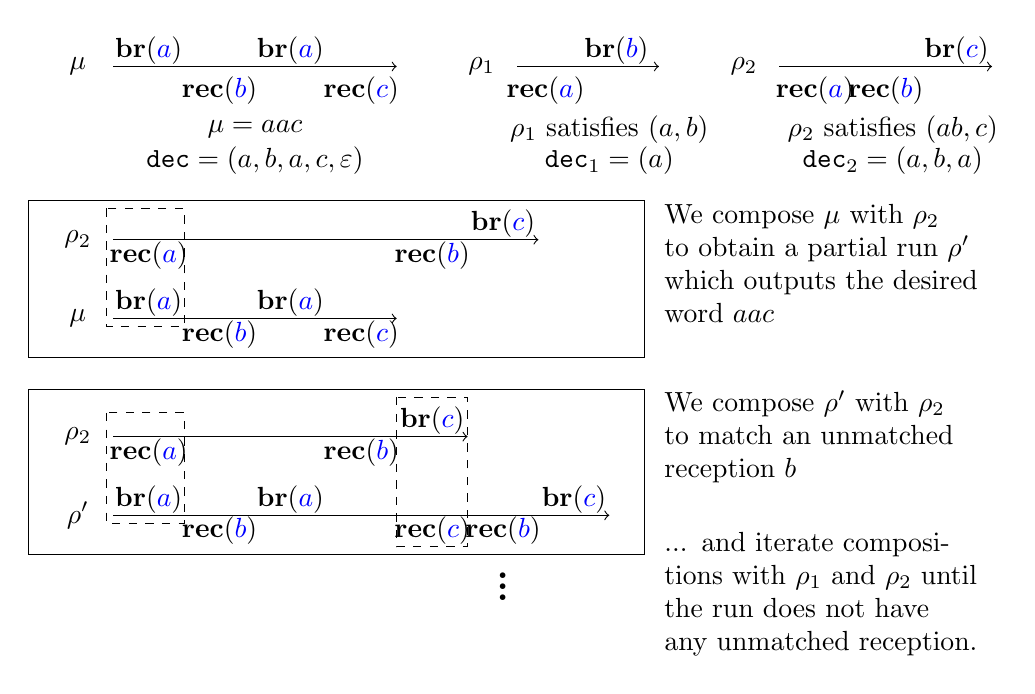
\begin{tikzpicture}[xscale=0.9]
	
	\draw[->] (-0.5,-1.8) -- (3.5,-1.8);
	\draw[->] (5.2,-1.8) -- (7.2,-1.8);
	\draw[->] (8.9,-1.8) -- (11.9,-1.8);
	
	\node (0) at (-1,-1.8) {$\localrunlabel{\node}$};
 	\node (1) at (4.7,-1.8) {$\run_1$};
 	\node (2) at (8.4,-1.8) {$\run_2$};


	\node (b) at (0,-1.6) {$\brone{\color{blue}a\color{black}}$};
	\node (b) at (1,-2.1) {$\recsymb({\color{blue}b\color{black}})$};
	\node (b) at (2,-1.6) {$\brone{\color{blue}a\color{black}}$};
	\node (b) at (3,-2.1) {$\recsymb({\color{blue}c\color{black}})$};
	
	\node (b) at (5.6,-2.1) {$\recsymb({\color{blue}a\color{black}})$};
	\node (b) at (6.6,-1.6) {$\brone{\color{blue}b\color{black}}$};
	
	\node (b) at (9.4,-2.1) {$\recsymb({\color{blue}a\color{black}})$};
	\node (b) at (10.4,-2.1) {$\recsymb({\color{blue}b\color{black}})$};
	\node (b) at (11.4,-1.6) {$\brone{\color{blue}c\color{black}}$};

	\node (1) at (1.5,-2.6) {$\bosslabel{\node}=aac$};
	\node (1) at (6.5,-2.6) {$\run_1 \text{ satisfies } (a,b)$};
	\node (1) at (10.5,-2.6) {$\run_2 \text{ satisfies } (ab,c)$};

	\node (1) at (1.5,-3) {$\decsymb = (a,b, a, c, \epsilon)$};
	\node (1) at (6.5,-3) {$\decsymb_1 = (a)$};
	\node (1) at (10.5,-3) {$\decsymb_2 = (a, b, a)$};

%	\draw[->] (-0.5,-3) -- (7.5,-3);
	\draw[->] (-0.5,-4) -- (5.5,-4);
	\draw[->] (-0.5,-5) -- (3.5,-5);
	\draw[dashed] (-0.6, -3.6) rectangle (0.5, -5.1);
	
	\node (b) at (0,-4.8) {$\brone{\color{blue}a\color{black}}$};
	\node (b) at (1,-5.2) {$\recsymb({\color{blue}b\color{black}})$};
	\node (b) at (2,-4.8) {$\brone{\color{blue}a\color{black}}$};
	\node (b) at (3,-5.2) {$\recsymb({\color{blue}c\color{black}})$};

%	\node (b) at (0,-3.2) {$\recsymb({\color{blue}a\color{black}})$};
%	\node (b) at (6,-3.2) {$\recsymb({\color{blue}b\color{black}})$};
%	\node (b) at (7,-2.7) {$\brone{\color{blue}c\color{black}}$};
	
	\node (b) at (0,-4.2) {$\recsymb({\color{blue}a\color{black}})$};
	\node (b) at (4,-4.2) {$\recsymb({\color{blue}b\color{black}})$};
	\node (b) at (5,-3.8) {$\brone{\color{blue}c\color{black}}$};
	
%	\node (0) at (-1,-3) {$\run_2$};
	\node (0) at (-1,-4) {$\run_2$};
	\node (0) at (-1,-5) {$\localrunlabel{\node}$};
	
	\draw (-1.7, -5.5) rectangle (7, -3.5);
	\node[text width =4cm] (txt2) at (9.5, -4.3) {We compose $\localrunlabel{\node}$ with $\run_2$ to obtain a "partial run" $\run'$ which outputs the desired word $aac$};
	
	\draw[->] (-0.5,-6.5) -- (4.5,-6.5);
	\draw[->] (-0.5,-7.5) -- (6.5,-7.5);
	\draw[dashed] (-0.6, -6.2) rectangle (0.5, -7.6);
	\draw[dashed] (3.5, -6) rectangle (4.5, -7.9);
	
	\node (b) at (0,-7.3) {$\brone{\color{blue}a\color{black}}$};
	\node (b) at (1,-7.7) {$\recsymb({\color{blue}b\color{black}})$};
	\node (b) at (2,-7.3) {$\brone{\color{blue}a\color{black}}$};
	\node (b) at (4,-7.7) {$\recsymb({\color{blue}c\color{black}})$};
	\node (b) at (5,-7.7) {$\recsymb({\color{blue}b\color{black}})$};
	\node (b) at (6,-7.3) {$\brone{\color{blue}c\color{black}}$};
%	\node (b) at (7,-7.7) {$\recsymb({\color{blue}b\color{black}})$};
%	\node (b) at (8,-7.3) {$\brone{\color{blue}c\color{black}}$};
	
	\node (b) at (0,-6.7) {$\recsymb({\color{blue}a\color{black}})$};
	\node (b) at (3,-6.7) {$\recsymb({\color{blue}b\color{black}})$};
	\node (b) at (4,-6.3) {$\brone{\color{blue}c\color{black}}$};
	
	\node (0) at (-1,-6.5) {$\run_2$};
	\node (0) at (-1,-7.5) {$\run'$};
	
	\draw (-1.7, -8) rectangle (7, -5.9);
%	\node (r') at (9.5, -7) {$\run''$};
	\node[text width = 4cm] (txt1) at (9.5, -6.5) {We compose $\run'$ with $\run_2$ to match an "unmatched reception" $b$};
	
%	\node (b) at (0,-9.8) {$\brone{\color{blue}a\color{black}}$};
%	\node (b) at (1,-10.2) {$\recsymb({\color{blue}b\color{black}})$};
%	\node (b) at (2,-9.8) {$\brone{\color{blue}a\color{black}}$};
%	\node (b) at (3,-10.2) {$\recsymb({\color{blue}b\color{black}})$};
%	\node (b) at (4,-9.8) {$\brone{\color{blue}c\color{black}}$};
%	\node (b) at (5,-10.2) {$\recsymb({\color{blue}b\color{black}})$};
%	\node (b) at (6,-9.8) {$\brone{\color{blue}c\color{black}}$};
%	\node (b) at (7,-10.2) {$\recsymb({\color{blue}b\color{black}})$};
%	\node (b) at (8,-9.8) {$\brone{\color{blue}c\color{black}}$};
%	
%	\node (b) at (0,-9.2) {$\recsymb({\color{blue}a\color{black}})$};
%	\node (b) at (7,-8.8) {$\brone{\color{blue}b\color{black}}$};
%	
%		\draw[->] (-0.5,-9) -- (7.5,-9);
%	\draw[->] (-0.5,-10) -- (8.5,-10);
%	\draw[dashed] (-0.6, -8.8) rectangle (0.5, -10.1);
%	\draw[dashed] (6.4, -8.6) rectangle (7.5, -10.4);
	
%	\node (0) at (-1,-9) {$\run_1$};
%	\node (0) at (-1,-10) {$\run''$};
%	
%	\draw (-1.7, -10.5) rectangle (9, -8.4);
%	\node (r') at (9.5, -7) {$\run''$};
%	\node (txt1) at (11.7, -9) {We compose $\run''$ with $\run_1$ to};
%	\node (txt2) at (11.7, -9.5) {eliminate the last $b$ input};
	
	\node (d) at (5,-8.3) {\Huge \vdots};
 	\node[text width=4cm] (d) at (9.5,-8.5) {... and iterate compositions with $\run_{1}$ and $\run_2$ until the "run" does not have any "unmatched reception".};
%	\node (b1) at (0,0.6) {};
%	\node (b2) at (1,0.6) {};
%	\node (b3) at (3,0.6) {};
%	\node (b4) at (5,0.6) {};
%	\node (b5) at (10,0.6) {};
%	
%	\node (sp) at (11,2) {\Large ``$\color{blue}abdb\color{black}$''};
%	
%	
%	\node (r) at (2,-0.5) {$\recsymb(\color{magenta}a\color{black})$};
%	\node (r) at (4,-0.5) {$\recsymb(\color{orange}b\color{black})$};
%	\node (r) at (6,-0.5) {$\recsymb(\color{blue}c\color{black})$};
%	\node (r) at (7,-0.5) {$\recsymb(\color{olive}d\color{black})$};
%	\node (r) at (8,-0.5) {$\recsymb(\color{orange}a\color{black})$};
%	\node (r) at (9,-0.5) {$\recsymb(\color{teal!80}a\color{black})$};
%	
%	\node (r1) at (2,-0.4) {};
%	\node (r2) at (4,-0.6) {};
%	\node (r3) at (6,-0.4) {};
%	\node (r4) at (7,-0.6) {};
%	\node (r5) at (8,-0.6) {};
%	\node (r6) at (9,-0.6) {};
%	
%	\node[draw] (f1) at (1,2) {$(\color{magenta}ab\color{black}, \color{magenta}a\color{black})$};
%	\node[draw] (f2) at (3.7,2) {$(\color{blue}ab\color{black}, \color{blue}c\color{black})$};
%	\node[draw] (f3) at (6.8,2) {$(\color{blue}abc\color{black}, \color{blue}d\color{black})$};
%	\node (fa1) at (1,1.8) {};
%	\node (fa'1) at (1.6,1.6) {};
%	\node (fa2) at (3.7,1.8) {};
%	\node (fa'2) at (4.2,1.8) {};
%	\node (fa3) at (6.8,1.8) {};
%	\node (fa'3) at (6.3,1.8) {};
%	
%	
%	\node[draw] (bo1) at (4.5,-2) {$\color{orange}ba\color{black}$};
%	\node[draw] (bo2) at (6.9,-2) {$\color{olive}d\color{black}$};
%	\node[draw] (bo3) at (8.8,-2) {$\color{teal!80}a\color{black}$};
%	
%	
%	\node (ba1) at (4.5,-1.8) {};
%	\node (ba2) at (6.9,-1.8) {};
%	\node (ba3) at (8.8,-1.8) {};
%	
%	\draw[color=magenta, ->, >=angle 45] (b1) ..controls +(0,0.5) and +(0,-1).. (fa1);
%	\draw[color=magenta, ->, >=angle 45] (b2) ..controls +(0,0.5) and +(0,-1).. (fa1);
%	
%	\draw[color=blue, ->, >=angle 45] (b3) ..controls +(0,0.5) and +(0,-1).. (fa2);
%	\draw[color=blue, ->, >=angle 45] (b4) ..controls +(0,0.5) and +(0,-1).. (fa2);
%	
%	\draw[color=blue, ->, >=angle 45] (b3) ..controls +(0,0.5) and +(0,-1).. (fa3);
%	\draw[color=blue, ->, >=angle 45] (b4) ..controls +(0,0.5) and +(0,-1).. (fa3);
%	
%	\draw[color=orange, ->, >=angle 45] (ba1) ..controls +(0,0.5) and +(0,-1).. (r2);
%	\draw[color=orange, ->, >=angle 45] (ba1) ..controls +(0,0.5) and +(0,-1).. (r5);
%	
%	\draw[color=olive, ->, >=angle 45] (ba2) ..controls +(0,0.5) and +(0,-1).. (r4);
%	\draw[color=teal, ->, >=angle 45] (ba3) ..controls +(0,0.5) and +(0,-1).. (r6);
%	
%	\draw[color=magenta, ->, >=angle 45, dashed] (fa'1) ..controls +(0,0.5) and +(0,1).. (r1);
%	\draw[color=blue, ->, >=angle 45, dashed] (fa'2) ..controls +(0.5,0) and +(0,1).. (r3);
%	\draw[color=blue, ->, >=angle 45, dashed] (fa'2) ..controls +(0.5,0) and +(-0.5,0).. (fa'3);
\end{tikzpicture}
	\caption{Illustration of Lemma~\ref{lem:follower-composition-output}}
	\label{fig:tree-to-run}
\end{figure}


\begin{lemma}
	\label{lem:follower-composition-output}
	Let $\decsymb = (w_0, m_1, \ldots, w_\ell)$ be a "decomposition", $w'_0, \ldots, w'_\ell \in \messages^*$ such that for all $i \in \nset{0}{\ell}$, the projection of $w'_i$ on $\messages\setminus \set{m_1, \ldots, m_{i-1}}$ is a subword of $w_i$.
	
	Let $\config_0, \ldots, \config_{\ell+1}$ be configurations and $v$ a value such that for all $j \in\nset{1}{\ell+1}$ there exists a "partial run" $\run_j$ from $\config_{j-1}$ to $\config_{j}$ with $w_j \subword \voutput{v}{\run_j}$ and $\vinput{v}{\run_j} \in \set{m_1,\ldots, m_{j-1}}^*$.
	
	Suppose that for all $j \in\nset{1}{\ell}$ there exists a "partial run" $\run'_j$ and a value $v_j$ such that $\vinput{v_j}{\run'_j} \in \langdec{\decsymb_j}$ where $\decsymb_j = (w_0, m_1, \ldots, w_{j-1})$, $\vinput{v'}{\run'_j} = \varepsilon$ for all $v' \neq v_j$ and the last step of $\run'_j$ is an internal message $\intmessage{m}{v_j}$.
	
	Then, there exist "configurations" $\Tilde{\config}_0, \ldots, \Tilde{\config}_{\ell+1}$ such that for all $j \in\nset{0}{\ell}$, there is a "partial run" $\Tilde{\run}_j$ from $\Tilde{\config}_j$ to $\Tilde{\config}_{j+1}$ and
\begin{itemize}
	\item $w'_j \subword \voutput{v}{\Tilde{\run}_j}$, 
	
	\item $\vinput{v}{\Tilde{\run}_j} = \varepsilon$,
	
	\item for all $v' \neq v$, if $\vproj{v'}{\run_j} \neq \varepsilon$ then $\vproj{v'}{\Tilde{\run}_j} = \vproj{v'}{\run_j}$
	
	\item for all $v' \neq v$, if $\vproj{v'}{\run_j} = \varepsilon$ then $\vinput{v'}{\Tilde{\run}_j} = \varepsilon$
\end{itemize}
\end{lemma}

\begin{proof}
	Let $w' = w'_0 \cdots w'_\ell$.
	We proceed by strong induction on $\size{w'}$.
	
	If for all $j$ we have $w'_j \subword w_j$  (and thus $w'_j \subword \voutput{v}{\run_j}$), the result is a direct consequence of Lemma~\ref{lem:follower-composition-completion}.
	
	Suppose it is not the case. Then there exists $j, j'$ such that $j' \leq j$ and $m_{j'}$ appears in $w'_j$. Let $w'_j = w^-_j m_{j'} w^+_j$ and let $w''_j$ be the word $w^-_jw^+_j$.
	
	Then, there exist "configurations" $\widehat{\config}_0, \ldots, \widehat{\config}_{\ell+1}$ such that for all $i \in\nset{0}{\ell}$, there is a "partial run" $\widehat{\run}_i$ from $\widehat{\config}_i$ to $\widehat{\config}_{i+1}$ and
\begin{itemize}
	\item $w'_i \subword \voutput{v}{\widehat{\run}_i}$ if $i \neq j$,
	
	\item $w''_j \subword \voutput{v}{\widehat{\run}_j}$ 
	
	\item $\vinput{v}{\widehat{\run}_i} = \varepsilon$,
	
	\item for all $v' \neq v$, if $\vproj{v'}{\run_i} \neq \varepsilon$ then $\vproj{v'}{\widehat{\run}_i} = \vproj{v'}{\run_i}$
	
	\item for all $v' \neq v$, if $\vproj{v'}{\run_j} = \varepsilon$ then $\vinput{v'}{\widehat{\run}_i} = \varepsilon$
\end{itemize}

From these runs we infer a sequence of "partial runs" that output $w'_0, \ldots, w'_\ell$ but have a non-empty $v$-input. We then use Lemma~\ref{lem:follower-composition-completion} to obtain the desired runs with an empty $v$-input.

We proceed in a similar manner as in Lemma~\ref{lem:follower-composition-completion}.
There exists a "partial run" $\run'_{j'}$ and a value $v_{j'}$ such that $\vinput{v_{j'}}{\run'_{j'}} \in \langdec{\decsymb_{j'}}$,  $\vinput{v'}{\run'_{j'}} = \varepsilon$ for all $v' \neq v_j$  and the last step of $\run'_{j'}$ is an internal message $\intmessage{m}{v_{j'}}$.

Hence $\run'_{j'}$ can be decomposed as $\config_{{j'},0} \pstep{\run_{{j'},1}'} \config_{{j'},1} \cdots \pstep{\run_{{j'},j'-1}'} \config_{{j'},j'} \intmessage{m_{j'}}{v} \config'_{j'}$ where, for all $i \in \nset{1}{j'-1}$, the projection of $\vinput{v_{j'}}{\run_{{j'},i}'}$ on ${\messages\setminus\set{m_1, \ldots, m_{{i}-1}}}$ is a subword of $w_i$.

We can rename agents so that the $\widehat{\run}_i$ and $\run'_{j',i}$ are on disjoint sets of agents, and apply a renaming of values in $\run'_{j'}$ so that $v_{j'}$ is mapped to $v$ and all other values are mapped to values that do not appear in $\run$.
We then construct a sequence of runs by executing in parallel $\run_{j',i}'$ and $\widehat{\run}_i$ for all $i\in\nset{1}{\ell}$. As $w_i \subword \voutput{v}{\widehat{\run}_i}$, we can match the "internal messages@@global" of $\widehat{\run}_i$ with some "external messages@@global" of $\run'_{j',i}$ so that the remaining "external messages@@global" with value $v$ in $\run'_{j',i}$ are all in $\set{m_1, \ldots, m'_{j'}}$. 
We obtain, for each $i \in \nset{1}{j'-1}$, a run $\run''_i$ from $\widehat{\config}_{i-1} \sqcup \config_{j', i-1}$ to $\widehat{\config}_{i} \sqcup \config_{j', i}$ with $\vinput{v}{\run''_i} \in \set{m_1, \ldots, m_{i-1}}^*$. 

For each $i \in \nset{j'+1}{j-1}$, let $\run''_i$ be the run that goes from $\widehat{\config}_{i-1} \sqcup \config_{j', j'}$ to $\widehat{\config}_{i} \sqcup \config_{j', j'}$ by executing $\widehat{\run}_i$ on the first part and staying idle on the second one.

We can split $\widehat{\run}$ into $\widehat{\config}_{j} \pstep{\widehat{\run}^-} \widehat{\config}^- \pstep{\widehat{\run}^+} \widehat{\config}_{j+1}$
Let $\run''_j$ be the run from $\widehat{\config}_{j-1} \sqcup \config_{j', j'}$ to $\widehat{\config}_{j} \sqcup \config'_{j'}$ obtained by executing $\widehat{\run}_{j}^-$ on the first part, then executing the last step of $\run'_{j'}$ to broadcast $m_{j'}$ with value $v$ and then executing $\run_{j}^+$ on the first part.

For each $i \in \nset{j+1}{\ell}$, let $\run''_i$ be the run that goes from $\widehat{\config}_{i-1} \sqcup \config'_{j'}$ to $\widehat{\config}_{i} \sqcup \config'_{j'}$ by executing $\run_i$ on the first part and staying idle on the second one.

Note that for all $i \in \nset{0}{\ell}$, for all $v' \neq v$, if $\vproj{v'}{\run_i} \neq \epsilon$ then $\vproj{v'}{\run''_i} = \vproj{v'}{\run_i}$ (as we renamed values so that $\run$ and $\run'_j$ use disjoint sets of values apart from $v$) and if $\vproj{v'}{\run_i} = \epsilon$ then $\vinput{v'}{\run''_i} = \vinput{v'}{\run'_{j',i}} = \epsilon$.

Note that for all $i$ we have $w'_i \subword \voutput{v}{\widehat{\run}_i}$
We can apply Lemma~\ref{lem:follower-composition-completion} to the $\widehat{\run}_i$ and the $w'_i$.

We obtain a sequence of runs $\Tilde{\run}_0, \ldots, \Tilde{\run}_\ell$ such that, for all $i\in\nset{0}{\ell}$:
\begin{itemize}
	\item $\voutput{v}{\widehat{\run}_i} \subword \voutput{v}{\Tilde{\run}_i}$
	
	\item $\vinput{v}{\Tilde{\run}_i} = \epsilon$
	
	\item for all $v' \neq v$, if $\vproj{v'}{\widehat{\run}_i} \neq \epsilon$ then $\vproj{v'}{\widehat{\run}_i} = \vproj{v'}{\Tilde{\run}_i}$
	
	\item for all $v' \neq v$, if $\vproj{v'}{\widehat{\run}_i} = \epsilon$ then  $\vinput{v'}{\Tilde{\run}_i} = \epsilon$.
\end{itemize}

As a result, we have the following properties for all $i$:
\begin{itemize}
	\item $w'_i \subword \voutput{v}{\widehat{\run}_i} \subword \voutput{v}{\Tilde{\run}_i}$
	
	\item $\vinput{v}{\Tilde{\run}_i} = \epsilon$
	
	\item for all $v' \neq v$, if $\vproj{v'}{\run_i} \neq \epsilon$ then $\vproj{v'}{\run_i} = \vproj{v'}{\widehat{\run}_i} = \vproj{v'}{\Tilde{\run}_i}$
	
	\item for all $v' \neq v$, if $\vproj{v'}{\run_i} = \epsilon$ then either $\vproj{v'}{\widehat{\run}_i} = \epsilon$ and thus $\vinput{v'}{\Tilde{\run}_i} = \epsilon$, or $\vproj{v'}{\widehat{\run}_i} \neq \epsilon$ and then $\vproj{v'}{\Tilde{\run}_i} = \vproj{v'}{\widehat{\run}_i}$, thus in particular $\vinput{v'}{\Tilde{\run}_i} = \vinput{v'}{\widehat{\run}_i} = \epsilon$. 
\end{itemize}

Hence the $\Tilde{\run}_i$ satisfy all the required conditions.
\end{proof}

We are now ready to prove Lemma~\ref{lem:tree-to-run}.

\LemTreeToRun*


	We prove the following statement by induction on the length of the longest branche in the "unfolding tree" $\tree$.  
	
	The induction property is as follows. For every "unfolding tree" $\tree$:
	\begin{itemize}
		\item if $\tree$ satisfies a "boss specification" $w \in \messages^*$, then there exists a run $\run$ satisfying $w$.
		\item if $\tree$ satisfies a "follower specification" $(\followwordspec, \followmessagespec)$ then there exists a "partial run" $\run$ and a value $v$ such that $\Input{\run} \in (\messages\times \set{v})^*$, $\vinput{v}{\run} \subword \followwordspec$, and $\voutput{v}{\run}$ contains $\followmessagespec$.
	\end{itemize}
	
	Let $\tree$ be a "unfolding tree", let $\node$ be its root.
	
	We see $u := \localrunlabel{\node}$ as a "partial run" with a single agent.
	We are going to compose $u$ with some runs given by the children of $\node$ to construct a run satisfying the properties above.
	Let $V$ be the set of values appearing in $u$ and $V_{init}$ be the set of "initial@@partial" values of $u$.
	
	
	\subsubsection{Step 1: "Non-initial@@partial" values}
	\label{sec:tree-to-run-step-one}
	
	We show the following statement by induction on $\size{V'}$. It expresses that we can complete $u$ into a "partial run" that does not require any input over its "non-initial@@partial" values. This is done by induction, using Lemma~\ref{lem:boss-composition} and the runs obtained via the "boss" children to eliminate the input of $u$ over each of its "non-initial@@partial" values without adding some input requirements on other values or modifying its behaviour over values that were previously there.
	
For all $V' \subseteq V \setminus (V_{init}\cup \set{\valuelabel{\node}})$, there exists a "partial run" $\run$ such that for all $v \in \nats$:
\begin{itemize}
	\item If $v \in V \setminus V'$ then $\vproj{v}{\run} = \vproj{v}{u}$
	
	\item If $v \in V' \cup \nats \setminus V$ then $\vinput{v}{\run} = \epsilon$
\end{itemize}  
	
	If $V' = \emptyset$ then this is clear as we can simply take $\run := \localrun$.
	
	Now suppose there exists $v \in V \setminus (V_{init}\cup \set{\valuelabel{\node}} \cup V')$. Let $V'' = V' \cup \set{v}$. By induction hypothesis (on $\size{V'}$) there exists a "partial run" $\run'$ such that for all $v' \in \nats$:
	\begin{itemize}
		\item If $v' \in V \setminus V''$ then $\vproj{v'}{\run} = \vproj{v'}{u}$
		
		\item If $v' \in (\nats \setminus V) \cup V''$ then $\vinput{v'}{\run} = \epsilon$
	\end{itemize}

	As $v \neq \valuelabel{\node}$, by condition~\ref{item:condition1_non_initial_value} $\node$ has a child $\node'$ such that $\vinput{v}{\localrunlabel{\mu}} \subword  \bosslabel{\node'}$.
	By induction hypothesis (on the "unfolding tree"), as the subtree rooted in $\mu'$ satisfies the "boss specification" $\vinput{v}{\mu}$, there exists a run $\run_v$ satisfying $\vinput{v}{\localrunlabel{\mu}}$.
	
	Let $v' \in \nats$ be such that $\vinput{v}{\localrunlabel{\node}} \subword \voutput{v'}{\run_v}$. 
	
	We apply Lemma~\ref{lem:boss-composition} to obtain a run $\Tilde{\run}$ such that 
		\begin{itemize}			
		\item $\vinput{v}{\Tilde{\run}} = \varepsilon$ 
		
		\item for all $v'' \neq v$, if $\vproj{v''}{\run} \neq \varepsilon$ then $\vproj{v''}{\Tilde{\run}} = \vproj{v''}{\run}$
		
		\item for all $v'' \neq v$, if $\vproj{v''}{\run} = \varepsilon$ then $\vinput{v''}{\Tilde{\run}} = \varepsilon$.
	\end{itemize}
	
	As a result, $\Tilde{\run}$ is a partial run satisfying the three requirements for $V''$.  This concludes our induction.
	
	In particular, with $V' = V\setminus (V_{init}\cup \set{\valuelabel{\node}})$, we obtain that there exists a run $\run$ such that,
	for all $v \in \nats$:
	\begin{itemize}
		\item $\voutput{v}{u} \subword \voutput{v}{\run}$
		
		\item If $v \in (V_{init}\cup \set{\valuelabel{\node}})$ then $\vproj{v}{\run} = \vproj{v}{u}$
		
		\item If $v \notin (V_{init}\cup \set{\valuelabel{\node}})$ then $\vinput{v}{\run} = \epsilon$
	\end{itemize}  
	
	\subsubsection{Step 2: "Initial@@partial" values}
	\label{sec:tree-to-run-step-two}
	
	We proceed in the same way as in the previous part: the goal is now to use the "partial runs" yielded by the "follower" children to eliminate, one by one, using Lemma~\ref{lem:follower-composition-completion}, the input over each "non-initial@@partial" value of $u$, except maybe for $\valuelabel{\node}$, which requires a special case.
	
	We show the following statement by induction on $\size{V'}$.
	
	For all $V'$ such that $V \setminus (V_{init} \cup \set{\valuelabel{\node}}) \subseteq V' \subseteq V \setminus \set{\valuelabel{\node}}$, there exists a "partial run" $\run'$ such that for all $v \in \nats$:
	\begin{itemize}		
		\item If $v \in V \setminus V'$ then $\vproj{v}{\run'} = \vproj{v}{u}$
		
		\item If $v \in V' \cup (\nats \setminus V)$ then $\vinput{v}{\run'} = \epsilon$
	\end{itemize}  

If $V' = V \setminus (V_{init} \cup \set{\valuelabel{\node}})$ then this is clear as we can simply take the run $\run$ constructed in Section~\ref{sec:tree-to-run-step-one}.

Now suppose there exists $v \in V \setminus (\set{\valuelabel{\node}} \cup V')$. Let $V'' = V' \cup \set{v}$. By induction hypothesis (on $\size{V'}$) there exists a "partial run" $\run'$ such that for all $v' \in \nats$:
\begin{itemize}
	\item If $v' \in V \setminus V''$ then $\vproj{v'}{\run} = \vproj{v'}{u}$
	
	\item If $v' \in (\nats \setminus V) \cup V''$ then $\vinput{v'}{\run} = \epsilon$
\end{itemize}

As $v \neq \valuelabel{\node}$, by condition~\ref{item:condition2_initial_value}, there exists a "decomposition" $\decsymb = (w_0, m_1, \ldots, m_\ell, w_\ell)$ such that $u$ can be split into successive local runs $u_0, \cdots, u_\ell$ so that for all $i \in \nset{1}{\ell}$, $w_i \subword \voutput{v}{u_i}$, $\vinput{v}{u_i} \in \set{m_0, \ldots, m_{i-1}}^*$ and $\node$ has a child $\node_i$ such that $\followlabelmessage{\mu_i} = m_i$ and $\followlabelword{\node_i} \in \langdec{\decsymb_i}$ with $\decsymb_i = (w_0, m_1, \ldots, w_{i-1})$.

By induction hypothesis (on the "unfolding tree"), for each $i \in\nset{1}{\ell}$ there exists a run $\run'_i$ and a value $v'_i$ such that $\vinput{v''}{\run'_i} = \epsilon$ for all $v'' \neq v_i'$, $\vinput{v'_i}{\run'_i} \subword \followlabelword{\node_i}$ and $\voutput{v'_i}{\run'_i}$ contains $\followlabelmessage{\node_i}$.

For each $i$ we consider the shortest prefix $\run''_i$ of $\run'_i$ ending with an "internal message@@global" $\intmessage{\followlabelmessage{\node_i}}{v'_i}$, we have that $\vinput{v'_i}{\run''_i} \subword \vinput{v'_i}{\run'_i} \subword \followlabelword{\node_i}$.

Furthermore, as $u$ can be split into $u_0, \cdots, u_\ell$ so that for all $i \in \nset{1}{\ell}$, $w_i \subword \voutput{v}{u_i}$ and $\vinput{v}{u_i} \in \set{m_0, \ldots, m_{i-1}}^*$, we can do the same for $\run$ as $v \in V_{init}$ and thus by definition of $\run$ we have $\vproj{v}{\run} = \vproj{v}{u}$.
Hence we obtain a sequence of runs $\run_0, \ldots, \run_\ell$ such that for all $i \in \nset{1}{\ell}$, $w_i \subword \voutput{v}{\run_i}$ and $\vinput{v}{\run_i} \in \set{m_0, \ldots, m_{i-1}}^*$.

We apply Lemma~\ref{lem:follower-composition-completion} to obtain a sequence of runs $\Tilde{\run}_0, \ldots, \Tilde{\run}_\ell$ such that, for all $i$, 
\begin{itemize}	
	\item $\vinput{v}{\Tilde{\run}_i} = \varepsilon$ 
	
	\item for all $v' \neq v$, if $\vproj{v}{\run_i} \neq \varepsilon$ then $\vproj{v'}{\Tilde{\run}} = \vproj{v'}{\run}$
	
	\item for all $v' \neq v$, if $\vproj{v}{\run} = \varepsilon$ then $\vinput{v''}{\Tilde{\run}} = \varepsilon$.
\end{itemize}

As a result, $\Tilde{\run}$ is a partial run satisfying the three requirements for $V''$.  This concludes our induction.

	In particular, with $V' = V\setminus \set{\valuelabel{\node}}$, we obtain that there exists a run $\widehat{\run}$ such that 
for all $v \in \nats$:
\begin{itemize}
	\item If $v = \valuelabel{\node}$ then $\vproj{v}{\widehat{\run}} = \vproj{v}{\run} = \vproj{v}{u}$
	
	\item If $v \neq \valuelabel{\node}$ then $\vinput{v}{\widehat{\run}} = \vinput{v}{\run} = \epsilon$
\end{itemize}  

\subsubsection{Step 3: $\valuelabel{\node}$}

In this final part, we use Lemma~\ref{lem:follower-composition-output} to complete the "partial run" previously obtained so that it has enough output on $\valuelabel{\node}$ to satisfy the specification of $\node$. In fact, if $\node$ is a "follower node", the "partial run" constructed so far suffices. If $\node$ is a "boss node", we need to apply Lemma~\ref{lem:follower-composition-output}.
	
In Section~\ref{sec:tree-to-run-step-two} we constructed a run $\widehat{\run}$ such that for all $v \in \nats$:
\begin{itemize}
	\item If $v = \valuelabel{\node}$ then $\vproj{v}{\widehat{\run}} = \vproj{v}{u}$
	
	\item If $v \neq \valuelabel{\node}$ then $\vinput{v}{\widehat{\run}} = \epsilon$
\end{itemize}  

We have two cases: either $\mu$ is a "boss node" or a "follower node".

If $\mu$ is a "boss node" then there exists a decomposition $\decsymb=(w_0, m_1, \ldots, w_\ell)$ such that $\bosslabel{\node} \in \langdec{\decsymb}$ and $u$ can be split into $u_0, \cdots, u_\ell$ so that for all $i \in \nset{1}{\ell}$, $w_i \subword \voutput{v}{u_i}$ and $\vinput{v}{u_i} \in \set{m_0, \ldots, m_{i-1}}^*$ and $\node$ has a child $\node_i$ such that $\followlabelmessage{\mu_i} = m_i$ and $\followlabelword{\node_i} \in \langdec{\decsymb_i}$, with $\decsymb_i = (w_0, m_1, \ldots, w_{i-1})$.

As $\bosslabel{\node} \in \langdec{\decsymb}$, we have $\bosslabel{\node} = w'_0 \cdots w'_\ell$ where for all $i$ the projection of $w'_i$ on $\messages\setminus\set{m_1, \ldots, m_{i-1}}$ is a subword of $w_i$. 

We repeat the arguments from Section~\ref{sec:tree-to-run-step-two}, but we use Lemma~\ref{lem:follower-composition-output} instead of Lemma~\ref{lem:follower-composition-completion} to obtain a run $\Tilde{\run}$ such that,
\begin{itemize}	
	\item $\vinput{v}{\Tilde{\run}} = \epsilon$ for all $v \in \nats$
	
	\item $\bosslabel{\node} \subword \voutput{\valuelabel{\node}}{\Tilde{\run}}$
\end{itemize}

If $\tree$ satisfies a "boss specification" $w$  then $w \subword \bosslabel{\node} $ and thus $w \subword \voutput{\valuelabel{\node}}{\Tilde{\run}}$.

As a result, $\Tilde{\run}$ satisfies $w$ as well.

If $\node$ is a "follower node" then the run $\widehat{\run}$ previously constructed is such that  

\begin{itemize}	
	\item $\vinput{v}{\Tilde{\run}} = \epsilon$ for all $v \neq \valuelabel{\node}$
	
	\item $\vinput{\valuelabel{\node}}{\widehat{\run}} = \voutput{\valuelabel{\node}}{\localrunlabel{\node}} \subword \followlabelword{\node}$
	
	\item $\voutput{\valuelabel{\node}}{\widehat{\run}} = \voutput{\valuelabel{\node}}{\localrunlabel{\node}}$ contains $\followlabelmessage{\node}$
\end{itemize}

Hence $\widehat{\run}$ satisfies the required properties.
This concludes our induction.



%	\section{Proofs of Lemma~\ref{lem:shortening-branches}}
\label{app:proofs-reduction-branches}
We prove the following two lemmas:

\begin{restatable}{lemma}{lemIncreasingBosses}
	\label{lem:increasing-bosses}
	Let $\tree$ be a "unfolding tree" satisfying a specification $\spec$.
	Let $\node, \node'$ be two "boss nodes" of $\tree$.
	If $\node$ is an ancestor of $\node'$ and $\bosslabel{\node}$ is a subword of $\bosslabel{\node'}$ then there exists a smaller "unfolding tree" satisfying $\spec$.  
\end{restatable}

\begin{restatable}{lemma}{lemIncreasingFollowers}
	\label{lem:increasing-followers}
	Let $\tree$ be a "unfolding tree" satisfying a specification $\spec$.
	Let $\node, \node'$ be two "follower nodes" of $\tree$.
	If $\node$ is an ancestor of $\node'$, $\followlabelword{\node'} \subword \followlabelword{\node}$ and $\followlabelmessage{\node'}=\followlabelmessage{\node}$ then there exists a smaller "unfolding tree" satisfying $\spec$. 
\end{restatable}


\lemIncreasingBosses*

\begin{proof}
	Let $\tree_{\node}$, $\tree_{\node'}$ be the subtrees rooted in $\node$, $\node'$ respectively. 
	Let $\tree'$ be the tree obtained by replacing $\tree_{\node}$ with $\tree_{\node'}$. The size of $\tree'$ is smaller than the one of $\tree$, as $\tree_{\node'}$ is a strict subtree of $\tree_{\node}$.
	
	If $\node$ is the root of $\tree$, then $\tree'$ is a "unfolding tree" with $\node'$ as root. As $\node$ is a "boss node" and $\tree$ satisfies $\spec$, $\spec$ is a "boss specification", and a subword of $\bosslabel{\node}$.
	As $\bosslabel{\node}$ is a subword of $\bosslabel{\node'}$, $\spec$ is a subword of $\bosslabel{\node'}$ and thus $\tree'$ satisfies $\spec$.
	
	If $\node$ is not the root of $\tree$ then let $\node''$ be its father. We have to check that $\tree'$ is a "unfolding tree". 
	All nodes other than $\node''$ have the same label and children as before, thus the conditions of "unfolding trees" are still respected for them.
	As for $\node''$, it has the same "follower" children, hence conditions \ref{unfoldingC1} and \ref{unfoldingC3.1} are respected. Condition \ref{unfoldingC2} only depends on its label, which hasn't changed.
	
	Finally, let $v'$ be a value that is not initial in $\localrunlabel{\node''}$. Either $\node''$ has a "boss" child other than $\node'$ such that $\vinput{v'}{\localrunlabel{\node''}}$ is a subword of its label, or $\vinput{v'}{\localrunlabel{\node''}}$ is a subword of $\bosslabel{\node}$, which is a subword of $\bosslabel{\node'}$, hence condition \ref{unfoldingC3.2} is satisfied. 
	
	As a result, in both cases $\tree'$ is a "unfolding tree" smaller than $\tree$ that satisfies $\spec$. 
\end{proof}

\lemIncreasingFollowers*

\begin{proof}
	Let $\tree_{\node}$, $\tree_{\node'}$ be the subtrees rooted in $\node$, $\node'$ respectively. 
	Let $\tree'$ be the tree obtained by replacing $\tree_{\node}$ with $\tree_{\node'}$. The size of $\tree'$ is smaller than the one of $\tree$, as $\tree_{\node'}$ is a strict subtree of $\tree_{\node}$.
	
	If $\node$ is the root of $\tree$, then $\tree'$ is a "unfolding tree" with $\node'$ as root. As $\node$ is a "follower node" and $\tree$ satisfies $\spec$, $\spec$ is a "follower specification". Let $(\followwordspec, \followmessagespec) = \spec$, we have $\followlabelword{\node} \subword \followwordspec$ and $\followlabelmessage{\node} = \followmessagespec$. 
	Hence we have $\followlabelword{\node'} \subword \followlabelword{\node} \subword \followwordspec $ and $\followlabelmessage{\node'} = \followlabelmessage{\node} = \followmessagespec$, thus $\tree'$ satisfies $\spec$.
	
	If  $\node$ is not the root of $\tree$ then let $\node''$ be the father of $\node$. We have to check that $\tree'$ is a "unfolding tree". 
	All nodes other than $\node''$ have the same children as before, thus the conditions of "unfolding trees" are still respected for them.
	As for $\node''$, it has the same "boss" children, hence condition \ref{unfoldingC3.2} is respected. Condition \ref{unfoldingC2} only depends on its label, which hasn't changed.
	
	For conditions \ref{unfoldingC1} and \ref{unfoldingC3.1}, we can check that they are still satisfied by observing that since $\followlabelword{\node'} \subword \followlabelword{\node}$, for all "decomposition" $\decsymb$, if $\followlabelword{\node} \in \langdec{\decsymb}$ then $\followlabelword{\node'} \in \langdec{\decsymb}$. One can see that both conditions are satisfied by using the same "decompositions" and applying this fact.
	
	As a result, in both cases $\tree'$ is a "unfolding tree" smaller than $\tree$ that satisfies $\spec$. 
\end{proof}


	\section{Proof of Lemma~\ref{lem:short-run-for-output}}
\label{app:tower-lemma}

We first prove the following result:

\begin{restatable}{lemma}{lemShortLocalRuns}
	\label{lem:short-local-runs}
	There exists a primitive recursive function $\towerfun(n,r)$ such that, for every protocol $\prot$ with $r$ registers per agent, for every "local run" $\localrun: (q, \localdata) \step{*} (q', \localdata')$ in $\prot$, for every $V \subseteq \nats$ finite such that $V$ contains all message values appearing in $\localrun$,  for every $\Vinit \subseteq V$, there exists a "local run" $\localrun': (q, \localdata) \step{*} (q', \localdata')$ such that, denoting by $\Vinit$ the set of initial values in $\localrun$, we have $\length{\localrun'} \leq \towerfun(\size{\prot} + \size{\Vinit},r)$ and:
	\begin{enumerate}
		\item \label{item:shorterrun_anyvalue} for all $\aval' \in \nats \setminus V$, there exists $\aval \in \nats \setminus \Vinit$ such that $\vinput{\aval'}{\localrun'}$ is a subword of $\vinput{\aval}{\localrun}$,
		\item \label{item:shorterrun_oldvalues} for all $\aval \in V$, $\vinput{\aval}{\localrun'}$ is a subword of $\vinput{\aval}{\localrun}$. 
		% \item by writing $V := \nats \setminus \set{\localdata_i(k) \mid k \in \nset{1}{\regnum}}$, for every $\aval' \in V$, there exists $\aval \in V$ such that $\vinput{\aval'}{\localrun'}$ is a subword of $\vinput{\aval}{\localrun}$.
	\end{enumerate}
		%  with an "input" $I$.
% 	Let $u_1, u_2, u_3$ be such that $u=u_1u_2u_3$.
% 	If $\size{u_2} > TOWER$, then there exists $u'_2$ with $|u_2'| \leq \towerfun(\prot)$ such that $u_1u'_2u_3$ is a local run of $\prot$ with smaller "input" than $u$. 
\end{restatable}
Intuitively, the set $V$ represents values that are already used somewhere and therefore cannot be used as fresh values, and $\Vinit$ represents values that other values should not copy because their behavior is special (this will later correspond to initial values of the run). However, because this lemma is meant to be applied to several parts of a run, we have to state it for any value for $V$ and $\Vinit$.  

\begin{figure}
	

	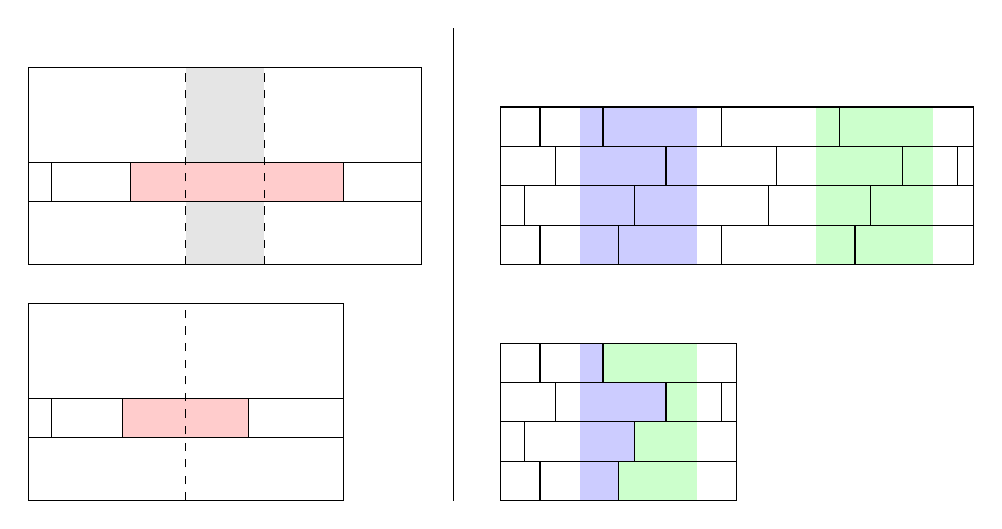
\begin{tikzpicture}
		\draw[white,fill=gray!20] (2,0) rectangle (3,0.8);
		\draw[white,fill=gray!20] (2,1.3) rectangle (3,2.5);
		
		\draw (0,0) rectangle (5,2.5);
		
		\draw (0,0.8) rectangle (5,1.3);
		
		\draw (0,0.8) rectangle (0.3,1.3);
		\draw (0,0.8) rectangle (1.3,1.3);
		\draw[fill=red!20] (1.3,0.8) rectangle (4,1.3);
		
		\draw[dashed] (2,0) -- (2,2.5);
		\draw[dashed] (3,0) -- (3,2.5);
		
		
		
		\draw (0,-3) rectangle (4,-0.5);
		
		\draw (0,-2.2) rectangle (4,-1.7);
		
		\draw (0,-2.2) rectangle (0.3,-1.7);
		\draw (0.3,-2.2) rectangle (1.3,-1.7);
		\draw[fill=red!20] (1.2,-2.2) rectangle (2.8,-1.7);
		
		\draw[dashed] (2,-3) -- (2,-0.5);
		
		\draw (5.4,-3) -- (5.4,3);
		
		
		\draw[white,fill=blue!20] (7,0) rectangle (8.5,2);
		\draw[white,fill=green!20] (10,0) rectangle (11.5,2);
		
		\draw (6,0) rectangle (12,2);
		
		\draw (6,0) rectangle (12,0.5);
		\draw (6,0) rectangle (12,1);
		\draw (6,0) rectangle (12,1.5);
		
		\draw (6,0) rectangle (6.5,0.5);
		\draw (6,0) rectangle (7.5,0.5);
		\draw (6,0) rectangle (8.8,0.5);
		\draw (6,0) rectangle (10.5,0.5);
		
		\draw (6,0.5) rectangle (6.3,1);
		\draw (6,0.5) rectangle (7.7,1);
		\draw (6,0.5) rectangle (9.4,1);
		\draw (6,0.5) rectangle (10.7,1);
		
		\draw (6,1) rectangle (6.7,1.5);
		\draw (6,1) rectangle (8.1,1.5);
		\draw (6,1) rectangle (9.5,1.5);
		\draw (6,1) rectangle (11.1,1.5);
		\draw (6,1) rectangle (11.8,1.5);
		
		\draw (6,1.5) rectangle (6.5,2);
		\draw (6,1.5) rectangle (7.3,2);
		\draw (6,1.5) rectangle (8.8,2);
		\draw (6,1.5) rectangle (10.3,2);
		
		
		\draw[white, fill=blue!20] (7,-3) rectangle (7.5,-2.5);
		\draw[white,fill=blue!20] (7,-2.5) rectangle (7.7,-2);
		\draw[white,fill=blue!20] (7,-2) rectangle (8.1,-1.5);
		\draw[white,fill=blue!20] (7,-1.5) rectangle (7.3,-1);
		
		\draw[white,fill=green!20] (7.5,-3) rectangle (8.5,-2.5);
		\draw[white,fill=green!20] (7.7,-2.5) rectangle (8.5,-2);
		\draw[white,fill=green!20] (8.1,-2) rectangle (8.5,-1.5);
		\draw[white,fill=green!20] (7.3,-1.5) rectangle (8.5,-1);
		
		
		
		\draw (6,-3) rectangle (9,-2.5);
		\draw (6,-3) rectangle (9,-2);
		\draw (6,-3) rectangle (9,-1.5);
		\draw (6,-3) rectangle (9,-1);
		
		\draw (6,-3) rectangle (6.5,-2.5);
		\draw (6,-3) rectangle (7.5,-2.5);
		
		\draw (6,-2.5) rectangle (6.3,-2);
		\draw (6,-2.5) rectangle (7.7,-2);
		
		\draw (6,-2) rectangle (6.7,-1.5);
		\draw (6,-2) rectangle (8.1,-1.5);
		\draw (6,-2) rectangle (8.8,-1.5);
		
		\draw (6,-1.5) rectangle (6.5,-1);
		\draw (6,-1.5) rectangle (7.3,-1);
		
	\end{tikzpicture}


	\caption{Illustration of the proof of Lemma~\ref{lem:short-local-runs}. We represent local runs as above, where Lines correspond to registers, and vertical separations are times at which a $\enregact$ operation is performed on that register. If one register $i$ keeps the same value for a long enough time (on the left), we apply the induction hypothesis to shorten the projection of the run on the other registers. As the value of $i$ does not change, the resulting run is still valid. If all registers change values often, say every $M$ steps (on the right), then if the run is long enough we can find two identical sequences of transitions during which all values are renewed twice. We can then obtain a shorter run by glueing them together as in the picture. The colored rectangles in the shortened runs correspond to fresh values that we introduce to make sure that all local disequality tests succeed.}
\end{figure}

\begin{proof}
	Given a "local run" $\localrun$, register $i$ is ""active"" in $\localrun$ if at least one $\quotemarks{\enregact}$ step on register $i$ is performed in $\localrun$. 
	
	We define the function $\towerfun(n,k)$ recursively as $\towerfun(n,0) = n+1$ and $\towerfun(n,k+1) = 2(\towerfun(n,k) +1) [(n+1)^{4(\towerfun(n,k)+1)} +1]$. This function is clearly primitive recursive, although non-elementary; it grows as a tower of exponentials of height $k$ where each floor of the tower is polynomial in $n$.
	% A straightforward induction allows one to bound (roughly) $\towerfun(n)(k)$ between the towers of exponentials
	% $n^{n^{{\scriptstyle\cdot^{\scriptstyle\cdot^{\scriptstyle\cdot^{\scriptstyle n}}}}}}$ and $(4n^8+2)^{(4n^8+2)^{\scriptstyle {~\cdot^{\scriptstyle~\cdot^{\scriptstyle~\cdot^{\scriptstyle (4n^8+2)}}}}}}$  of height $k+1$.
	
	Let $n:=\size{\prot} + \size{\Vinit}$.
	We prove the ""shortening property"": \\
	Let a "local run" $\localrun: (q_i, \localdata_i) \step{*} (q_f, \localdata_f)$ with $k$ "active registers" such that $\length{\localrun} > \towerfun(n,k)$ and let $V \subseteq \nats$ finite that contains every message value appearing in $\localrun$. We claim that $\localrun$ can be shortened into a local run $\localrun': (q_i, \localdata_i) \step{*} (q_f, \localdata_f)$ with $k$ active registers such that $\length{\localrun'} < \length{\localrun}$ and:
	\begin{itemize}
		\item for all $\aval' \in \nats$, there exists $\aval \in \nats$ such that $\vinput{\aval'}{\localrun'}$ is a subword of $\vinput{\aval}{\localrun}$,
		\item for all $\aval \in V$, $\vinput{\aval}{\localrun'}$ is a subword of $\vinput{\aval}{\localrun}$. 
	\end{itemize}
	
	We proceed by induction on the number $k$ of "active registers" in the "local run". If $k=0$, register values do not change in $\localrun$. As $\towerfun(n,0) = n+1 \geq \size{Q}+1$, $\localrun$ goes through the same state twice, hence all steps in between may be removed. 
	
	Suppose that the property is true for any protocol with $\leq k$ "active registers", and consider a run $\localrun: (q_i,\localdata_i) \step{*} (q_f,\localdata_f)$ with $k+1$ "active registers" such that $\length{\localrun} > \towerfun(n,k+1)$.
	
	First, if there exists an infix "local run" $\localrun_i$ of $\localrun$ of length $\towerfun(n,k)+1$ with only $k$ active registers, then it suffices to apply the induction hypothesis on $u_i$ and $V$.
	
	Suppose now that there exists no such infix "local run".
	Let $I \subseteq \nset{1}{r}$ the set of "active registers" in $\localrun$, $|I| = k+1$. Let $M:= \towerfun(n,k){+}1$, we have $\towerfun(n,k+1) = 2M [((n+1)^2)^{2M}+1]$. 
	In any sequence of $M$ "local steps" in a row in $\localrun$, 
	there is a $\quotemarks{\enregact}$ transition on every register in $I$. Suppose that $\length{\localrun} > \towerfun(n,k+1)$. Additionally, suppose that  no local configuration appears twice in $\localrun$ (otherwise $\localrun$ may easily be shortened). 
	
	
	For every $i$, let $\atrans_i$ the $i$-th transition in $\localrun$, and let $\theta_i\in \Vinit \cup \set{\bot}$ be such that 
	\[
	\theta_i = 
	\begin{cases}
		& 	v \text{ if the $i$th step of $u$ is a "reception step" $\extlabel{\delta_i}{v}$ with $v \in \Vinit$ } \\ 
		& 	\bot \text{ otherwise}
	\end{cases}
	\]

	For every $i \in \nset{0}{(n+1)^{2M}}$, we write $s_i$ the sequence $\delta_{2  M \cdot i+1}, \delta_{2  M \cdot i+2}, \cdots, \delta_{2 M \cdot i+2M}$ and $\Theta_i$ the sequence $\theta_{2  M \cdot i}, \theta_{2 M \cdot i+1}, \cdots, \theta_{2 M \cdot i+2M}$.
	There are $|\transitions|^{2M}$ possible sequences for $s_i$ and $[\size{\Vinit} +1]^{2M}$ possible sequences for $\Theta_i$.
	By the pigeonhole principle there exist two indices $i_a, i_b$ such that the sequences $s_{i_a}$ and $s_{i_b}$ are equal and also the sequences $\Theta_{i_a}$ and $\Theta_{i_b}$ are equal (as $|\transitions| (\size{\Vinit}+1) \leq (n+1)^2$). 
	There exist two infix "local runs" $\localrun_a: (q_1, \localdata_1) \step{*} (q_2, \localdata_2)$, $\localrun_b: (q_3, \localdata_3) \step{*} (q_4, \localdata_4)$ in $\localrun$ such that $(q_2,\localdata_2)$ appears strictly before $(q_3,\localdata_3)$ in $\localrun$ and $\localrun_a$ and $\localrun_b$ both have the same sequences of transitions, which we call $s$, and of receptions of values from $\Vinit$, which we call $\Theta$.
	
	Although $\localrun_a$ and $\localrun_b$ have the same sequence of transitions, their "traces" may differ because their "reception steps" may have different values.
	We build a "trace" $\atrace$ such that $(q_1,\localdata_1) \step{\atrace} (q_4, \localdata_4)$ where the underlying sequence of transitions of $\atrace$ is $s$ and the receptions of values of $\Vinit$ matches $\Theta$.
	
	For every active register $i \in I$, let $e_i \in \nset{1}{2M}$ denote the index of the first $\quotemarks{\enregact}$ on register $i$ in $s$ and $f_i \in \nset{1}{2M}$ the index of the last $\quotemarks{\enregact}$ on register $i$ in $s$. By hypothesis, because $s$ is of length $2M$, it contains at least two $\quotemarks{\enregact}$ on register $i$, one in the first half and one in the second half, hence $e_i \leq M < M +1 \leq f_i$. 
	
	For every $j \in \nset{1}{2M}$, let $\delta_j$ denote the $j$-th transition of $s$. First, if  $\delta_j$ is a "broadcast" or a "local test", we define the $j$-th "local step" of $\atrace$ as $\intlabel{\delta_j}$. 
	Suppose now that $\delta_j$ is a "reception" of the form $\rec{\amessage}{i}{\anact}$. The $j$-th "local step" of $\localrun_a$ (resp. $\localrun_b$) has underlying transition $\delta_j$ hence is an "reception step" of the form $\extlabel{\delta_j}{\aval_a}$ for some $\aval_a \in V$ (resp. $\extlabel{\delta_j}{\aval_b}$ for some $\aval_b \in V$).
	Because $V$ is finite and $\Vinit \subseteq V$, there exists an injective function $\phi: V \rightarrow \nats$ such that for all $v \in \Vinit$, $\phi(v) = v$ and for all $v \notin \Vinit$, $\phi(v) \notin V$.
	We define the $j$-th "local step" of $\atrace$ to be $\extlabel{\delta_j}{\aval}$ where:
	\begin{itemize}
		\item if $i \notin I$ then its value stays the same throughout $\localrun$, then we set $\aval = \aval_a (= \aval_b)$ 
		\item if $i \in I$ then  
		\begin{itemize}
			\item if $j < e_i$, $\aval = \aval_a$,
			\item if $e_i \leq j < f_i$, $\aval = \phi(\aval_a)$,
			\item if $f_i \leq j$, $\aval = \aval_b$.
		\end{itemize}
	\end{itemize}
	We now claim that $(q_1,\localdata_1) \step{\atrace} (q_4,\localdata_4)$. 
	First, for every active register $i$, the last $\quotemarks{\enregact}$ step on register $i$ has value $\localdata_4(i)$ in $\atrace$ (as we are in the case $f_i \leq j$). Hence if every "local step" is valid then the final "local configuration" is $(q_4, \localdata_4)$.
	For every $l \in \nset{0}{2M}$, let $\atrace_l$ denote the prefix of $\atrace$ of length $l$.
	We prove by induction on $l$ that $\atrace_l$ is valid from $(q_1, \localdata_1)$. It is trivially true for $l =0$. Assume that we have $(q_1, \localdata_1) \step{\atrace_l} (q, \localdata)$ and let $\locallabel$ such that $\atrace_l \cdot \locallabel = \atrace_{l+1}$. Let $\atrans$ the underlying transition of $\locallabel$.
	First, $q$ is the initial state of $\atrans$ because $\locallabel$ is valid at step $l+1$ of $\localrun_a$ (and $\localrun_b$). Hence if $\atrans$ is a "broadcast" then $\locallabel$ is valid from $(q,\localdata)$.
	
	For every register $i$, let $\localdata_a(i), \localdata_b(i)$ the content of register $i$ after the $l$-th step in $\localrun_a$ and $\localrun_b$ respectively.
	
	\noindent \textbf{$\locallabel$ is an "reception step"} \\
	If $\locallabel$ is an "reception step" of the form $\extlabel{\atrans}{\aval}$, then $\atrans$ has action $\rec{\amessage}{i}{\anact}$. Let $\aval_a$, $\aval_b$ the value of the corresponding "reception step" in $\localrun_a$ and $\localrun_b$ respectively. If $i \notin I$ then $\alpha$ is either $\quotemarks{\dummyact}$ or a test, which is valid as  $\localdata(i) = \localdata_a(i) = \localdata_b(i)$.
	
	The only problematic cases are when $i \in I$ and either $\anact = \quotemarks{\diseqtestact}$ or $\anact = \quotemarks{\eqtestact}$. 
	
	In this case, we prove that $\binrel{\aval}{\anact}{\localdata(i)}$ with $\anact \in \set{\quotemarks{\eqtestact}, \quotemarks{\diseqtestact}}$. First, because the corresponding step is valid in $\localrun_a$ and $\localrun_b$, we have $\binrel{\localdata_a(i)}{\anact}{\aval_a}$ and $\binrel{\localdata_b(i)}{\anact}{\aval_b}$. We distinguish cases depending on the value of $l+1$:
	\begin{itemize}
		\item $l+1<e_i$: $\localdata(i)= \localdata_a(i)$, $\aval = \aval_a$ and $\binrel{\localdata_a(i)}{\anact}{\aval_a}$. 
		\item $e_i \leq l+1 < f_i$: We have $\aval = \phi(\aval_a)$. 
		Moreover, because $e_i < l+1$, there is at least one $\quotemarks{\enregact}$ on register $i$ in $\atrace_l$. Consider the last such "transition" in $\atrace_l$; its index $j$ satisfies $e_i \leq j < f_i$ by definition of $e_i$, hence the value of the corresponding "reception step" in $\localrun_a$ is $\localdata_a(i)$ and its value in $\atrace_{l}$ is $\phi(\localdata_a(i))$. One has $\binrel{\localdata_a(i)}{\anact}{\aval_a}$ therefore (by injectivity of $\phi$ for $\anact = \quotemarks{\diseqtestact}$)
		$\binrel{\phi(\localdata_a(i))}{\anact}{\phi(\aval_a)}$.
		\item$f_i \leq l+1$: $\localdata(i)= \localdata_b(i)$ and $\aval = \aval_b$, and because the "internal step" is valid in $\localrun_b$ we have $\binrel{\localdata_b(i)}{\anact}{\aval_b}$. 
	\end{itemize}
	
	\noindent \textbf{$\locallabel$ is an "internal step"} \\
	The only problematic case is when $\locallabel =: \loc{i}{i'}{\diseqtestact}$ with $i,i' \in \nset{1}{\regnum}$ (we have no local equality tests thanks to Proposition~\ref{prop:loc-eq-test-elimination}). We have to prove that $\localdata(i) \ne \localdata(i')$. 
	Because the "local test" is satisfied in $\localrun_a$ and $\localrun_b$, we have $\localdata_a(i) \ne \localdata_a(i')$ and $\localdata_b(i) \ne \localdata_b(i')$.
	
	If $i \notin I$ and $i' \notin I$ (none are "active registers") then  $\localdata(i) = \localdata_a(i) \ne \localdata_a(i') = \localdata(i')$.
	
	If $i \in I$ and $i' \notin I$, then $\localdata(i') = \localdata_a(i') = \localdata_b(i')$ and:
	\begin{itemize}
		\item if $l+1<e_i$ then $\localdata(i) = \localdata_a(i) \ne \localdata_a(i')$,
		\item if $e_i \leq l+1 < f_i$ then $\localdata(i) = \phi(\localdata_a(i))$ and either
		\begin{itemize}
			\item $\localdata_a(i) \in \Vinit$ hence $\localdata(i) = \phi(\localdata_a(i)) = \localdata_a(i) \neq \localdata_a(i')$
			
			\item $\localdata(i') \notin \Vinit$ therefore $\phi(\localdata_a(i)) \notin V$ and, as $\localdata(i') = \localdata_a(i') \in V$,  $\localdata(i) \ne \localdata(i')$
		\end{itemize}
		\item if $f_i \leq l+1$ then $\localdata(i) = \localdata_b(i) \ne \localdata_b(i')$.
	\end{itemize}
	We treat the case $i \notin I$ and $i' \in I$ symmetrically.
	
	If $i \in I$ and $i' \in I$, recall that $e_i \leq M < f_{i'}$ and $e_{i'} \leq M < f_i$ thus $e_i < f_{i'}$ and $e_{i'}< f_i$. We again make a case disjunction on the value of $l+1$:
	\begin{itemize}
		\item $l+1<e_i$ and $l+1 <e_{i'}$: $\localdata(i)= \localdata_a(i)$, $\localdata(i')= \localdata_a(i')$ and $\localdata_a(i) \ne \localdata_a(i')$. 
		
		\item $e_i \leq l+1 < f_i$, $l+1<e_{i'}$: $\localdata(i) = \phi(\localdata_a(i))$ and either
		\begin{itemize}
			\item $\localdata_a(i) \in \Vinit$, hence $\localdata(i) = \phi(\localdata_a(i)) = \localdata_a(i) \neq  \localdata_a(i') = \localdata(i')$, or
			
			\item $\localdata_a(i) \notin \Vinit$, hence $\phi(\localdata_a(i)) \notin V$, and $\localdata(i') = \localdata_a(i') \in V$ therefore $\localdata(i') \ne \localdata(i)$.
		\end{itemize}
		
		\item $e_{i'} \leq l+1 < f_{i'}$, $l+1<e_{i}$: symmetric to the previous case.
		
		\item $e_i \leq l+1 < f_i$, $e_{i'} \leq l+1 < f_{i'}$: $\localdata(i) = \phi(\localdata_a(i))$, $\localdata(i') = \phi(\localdata_a(i'))$; however $\localdata_a(i) \ne \localdata_a(i')$ and $\phi$ is injective hence $\localdata(i') \ne \localdata(i)$.
		
		\item $e_i \leq l+1 < f_i$, $f_{i'} \leq l+1$: $\localdata(i') = \localdata_b(i') \in V$, $\localdata(i) = \phi(\localdata_a(i))$  and either
		\begin{itemize}
			\item $\localdata_a(i) \in \Vinit$, in which case $\localdata_a(i) = \localdata_b(i)$ because $\theta_{i_a} = \theta_{i_b}$ ($\localrun_a$ and $\localrun_b$ coincide on values in $\Vinit$) hence $\localdata(i) = \phi(\localdata_a(i)) = \phi(\localdata_b(i)) = \localdata_b(i) \neq  \localdata_b(i') = \localdata(i')$, or
			\item $\localdata_a(i) \notin \Vinit$, hence $\phi(\localdata_a(i)) \notin V$, and $\localdata(i') = \localdata_b(i') \in V$ therefore $\localdata(i') \ne \localdata(i)$.
		\end{itemize}
		
		
		\item $f_i \leq l+1$, $e_{i'} \leq l+1 < f_{i'}$: symmetric to the previous case.
		
		\item $f_i \leq l+1$, $f_{i'} \leq l+1$: $\localdata(i)= \localdata_b(i)$, $\localdata(i)= \localdata_b(i)$ and $\localdata_b(i) \ne \localdata_b(i')$. 
	\end{itemize}
	
	This proves that $\locallabel$ is valid from $(q,\localdata)$ which concludes the induction. 
	We have proven that $(q_1,\localdata_1) \step{\atrace} (q_4, \localdata_4)$; moreover $\atrace$ is of length $2M$ and there are at least $2M+1$ steps between $(q_1,\localdata_1)$ and $(q_4, \localdata_4)$ in $\localrun$. Therefore, replacing this part of $\localrun$ with $(q_1,\localdata_1) \step{\atrace} (q_4, \localdata_4)$ yields a "local run" $\localrun': (q_i, \localdata_i) \step{*} (q_f,\localdata_f)$ with strictly less steps that $\localrun$. 
	
	It remains to prove the conditions on the "$v$-inputs" of $\localrun'$. If suffices to prove the condition for the part between $(q_1, \localdata_1)$ to $(q_4, \localdata_4)$,
	because the rest of $\localrun$ is left untouched. 
	
	Let $(q_m, \localdata_m)$ the "local configuration" after $M$ steps of $\atrace$ from $(q_1, \localdata_1)$; write $\localrun_1$ the local run from $(q_1,\localdata_1)$ to $(q_m, \localdata_m)$ corresponding to the first $M$ steps of $\atrace$ in $\localrun'$, and $\localrun_2$ the "local run" from $(q_m, \localdata_m)$ to $(q_4, \localdata_4)$ corresponding to the last $M$ steps of $\atrace$ in $\localrun'$.  
	
	Let $\aval \in V$. We claim that $\vinput{\aval}{\localrun_{1}}$ is a subword of $\vinput{\aval}{\localrun_a}$ and $\vinput{\aval}{\localrun_{2}}$ is a subword of $\vinput{\aval}{\localrun_b}$. Indeed, in the construction of $\atrace$, the "reception steps" in the first $M$ steps were those of $\localrun_a$ except that some values were replaced with fresh values in $\nats \setminus V$, and similarly with $\localrun_b$ and the last $M$ steps. Overall, this proves that $\vinput{\aval}{\localrun'}$ is a subword of $\vinput{\aval}{\localrun}$ for every $\aval \in V$ and values of $V$ satisfy conditions \ref{item:shorterrun_anyvalue} and \ref{item:shorterrun_oldvalues}. 
	
	Let $\aval' \in \nats \setminus V$; $\aval'$ does not appear in $\localrun$. Either $\aval'$ does not appear in $\localrun'$ in which case the desired property is true, or there exists $\aval \in V$ such that $\aval' = \phi(\aval)$. As $\phi$ is injective and $\phi(\Vinit) = \Vinit$ and $\aval'\notin \Vinit$, $\aval \notin \Vinit$. 
	But then $\vinput{\aval'}{\localrun_{1}}$ is a subword of $\vinput{\aval}{\localrun_a}$ and $\vinput{\aval'}{\localrun_{2}}$ is a subword of $\vinput{\aval}{\localrun_b}$. Indeed, in $\localrun_1$, the "reception steps" with value $\phi(\aval)$ correspond to "reception steps" in $\localrun_a$ with value $\aval$, and similarly for $\localrun_2$ and $\localrun_b$. This proves condition \ref{item:shorterrun_anyvalue} for every $\aval' \in \nats \setminus V$.
	Overall, we have proven the existence of a "local run" $\localrun': (q_i,\localdata_i) \step{*} (q_f,\localdata_f)$ that satisfies conditions \ref{item:shorterrun_anyvalue} and \ref{item:shorterrun_oldvalues} and that is strictly shorter that $\localrun$, which proves the "shortening property".
	
	We build a "local run" of length less that $\towerfun(\size{\prot}+\size{\Vinit},\regnum)$ as follows. We start with $\localrun^{(0)} := \localrun$ and $V^{(0)}$ the set of values of messages appearing in $\localrun^{(0)}$. For every $k$ such that $\length{\localrun^{(0)}} > \towerfun(\size{\prot}+\size{\Vinit},\regnum)$, we apply the "shortening property" on $\localrun^{(k)}$ and $V^{(k)}$ to obtain $\localrun^{(k+1)}$ and define $V^{(k+1)}$ by $V^{(k)} \cup W$ where $W$ is the set of values of messages in $\localrun^{(k+1)}$, which is finite.
	The construction stops when $\length{\localrun^{(k)}} \leq \towerfun(\size{\prot} + \size{\Vinit},\regnum)$, which concludes the proof of Lemma~\ref{lem:short-local-runs}. 
\end{proof}

We now prove the following, stronger version of Lemma~\ref{lem:short-run-for-output}.

\begin{lemma}
There exists a primitive recursive function $\towerfun(n,r)$ such that, for every protocol $\prot$ with $r$ registers per agent, for every "local run" $\localrun: (q, \localdata) \step{*} (q', \localdata')$ in $\prot$, for every $V \subseteq \nats$ finite such that $V$ contains all message values appearing in $\localrun$,  for every $\Vinit \subseteq V$, there exists a "local run" $\localrun': (q, \localdata) \step{*} (q', \localdata')$ such that $\length{\localrun'} \leq \towerfun(\size{\prot}+\size{\Vinit}, \regnum) (\size{w_{out}}+1)$, $w_{out} \subword \Output{\localrun'}$ and:
	\begin{enumerate}
		\item for all $\aval' \in \nats \setminus V$, there exists $\aval \in \nats\setminus \Vinit$ such that $\vinput{\aval'}{\localrun'}$ is a subword of $\vinput{\aval}{\localrun}$,
		\item for all $\aval \in V$, $\vinput{\aval}{\localrun'}$ is a subword of $\vinput{\aval}{\localrun}$. 
	\end{enumerate}
\end{lemma}

\begin{proof}
	We set $\towerfun$ to be the same function as in Lemma~\ref{lem:short-local-runs}. 
	Let $n = \size{\prot} + \size{\Vinit}$.
	
	We proceed by induction on $\size{w_{out}}$.
	If $w_{out} = \epsilon$ we simply apply Lemma~\ref{lem:short-local-runs}.
	
	Otherwise let $w'_{out} (m,v) = w_{out}$.
	As $w_{out} \subword \Output{\localrun}$ we can split $\localrun$ in three $\localrun_0: (q, \localdata) \step{*} (q_0, \nu_0)$, $(q_0, \localdata_0) \intstep{\delta} (q_1, \localdata_1)$, $\localrun_1 :(q_1, \localdata_1) \step{*} (q', \localdata')$ where $\delta$ applies a broadcast operation $\br{m}{i}$ and $\nu_{0} (i) = v$.
	
	Let $V \subseteq \nats$ finite that contains every message value appearing in $\localrun$, and thus in particular every message value appearing in $\localrun_0$.
	By induction hypothesis applied to $\localrun_0$, $V$ and $\Vinit$, there exists a "local run" $\localrun_0': (q, \localdata) \step{*} (q_0, \localdata_0)$ such that $\length{\localrun_0'} \leq (\towerfun(\size{\prot}+ \size{\Vinit},r)+1)\size{w'_{in}}$, $w'_{in} \subword \Output{\localrun_0'}$ and:
	
	\begin{enumerate}
		\item for all $\aval' \in \nats \setminus V$, there exists $\aval \in \nats \setminus \Vinit$ such that $\vinput{\aval'}{\localrun_0'}$ is a subword of $\vinput{\aval}{\localrun_0}$,
		\item for all $\aval \in V$, $\vinput{\aval}{\localrun_0'}$ is a subword of $\vinput{\aval}{\localrun_0}$. 
	\end{enumerate}
	
	We set $V'$ as the set of values that either are in $V$ or appear in $\localrun_0'$.
	By Lemma~\ref{lem:short-local-runs} applied to $\localrun_0$, $V'$ and $\Vinit$, there exists a "local run" $\localrun_1': (q_1, \localdata_1) \step{*} (q', \localdata')$ such that $\length{\localrun_1'} \leq \towerfun(\size{\prot}+ \size{\Vinit},r)-1$ and:
	\begin{enumerate}
		\item for all $\aval' \in \nats \setminus V'$, there exists $\aval \in \nats \setminus \Vinit$ such that $\vinput{\aval'}{\localrun_1'}$ is a subword of $\vinput{\aval}{\localrun_1}$,
		\item for all $\aval \in V'$, $\vinput{\aval}{\localrun_1'}$ is a subword of $\vinput{\aval}{\localrun_1}$. 
	\end{enumerate}
	
	Let $\localrun'$ be the concatenation of $\localrun'_0$, $(q_0, \localdata_0) \intstep{\delta} (q_1, \localdata_1)$ and $\localrun'_1$. As $w'_{in} \subword \Output{\localrun'_0}$, we have $w_{in} \subword \Output{\localrun}$.
	The length of $\localrun'$ is $\length{\localrun'_0} + 1 + \length{\localrun'_1}$, which is at most $(\towerfun(\size{\prot},r)+1)\size{w'_{in}} + \towerfun(\size{\prot},r) = \towerfun(\size{\prot},r)\size{w_{in}}$.
	
	Moreover, for all $v' \in \nats$, 
	\begin{itemize}
		\item if $v'\in V$, and then $\vinput{v'}{\localrun_0'} \subword \vinput{v'}{\localrun_0}$ and $\vinput{v'}{\localrun_1'} \subword \vinput{v'}{\localrun_1}$, thus $\vinput{v'}{\localrun'} \subword \vinput{v'}{\localrun}$.
		
		\item if $v' \in V' \setminus V$, then $v'$ does not appear in $\localrun$ and there exists $v \in \nats\setminus \Vinit$ such that $\vinput{v'}{\localrun_0'} \subword \vinput{v}{\localrun_0}$. Further, as $v' \in V'$ we have $\vinput{v'}{\localrun_1'} \subword \vinput{v'}{\localrun_1} = \epsilon$, hence $\vinput{v'}{\localrun'} \subword \vinput{v}{\localrun}$.
		
		\item if $v' \in \nats \setminus V'$, then by definition of $V'$ we have $\vinput{v'}{\localrun_0'} = \epsilon$, and there exists $v \in \nats \setminus \Vinit$ such that $\vinput{v'}{\localrun_1'} \subword \vinput{v}{\localrun_1}$, hence $\vinput{v'}{\localrun'} \subword \vinput{v}{\localrun}$.
	\end{itemize}
	This concludes our proof.
\end{proof}

To prove Lemma~\ref{lem:short-run-for-output}, we apply the previous lemma with $\Vinit$ the set of initial values of $\localrun$ and observe that this gives $\size{\Vinit} \leq \regnum$.









\begin{lemma}
	\label{lem:short-dec}
	Let $\decsymb = (w_0, m_1, \ldots, w_\ell)$ be a decomposition, and for all $i\in \nset{0}{\ell}$ let $\decsymb_i = (w_0, m_1, \ldots, w_i)$.
	Let $w'_0, \ldots, w'_\ell$ be such that $w'_i \in \langdec{\decsymb_i}$ for all $i$.
	
	Then there exists $\widehat{\decsymb} = (\widehat{w}_0, m_1, \ldots, \widehat{w}_\ell)$ such that, for all $i$, $\widehat{w}_i \subword w_i$ and $w'_i \in \langdec{\widehat{\decsymb}_i}$ (where $\widehat{\decsymb}_i = (\widehat{w}_0, m_1, \ldots, \widehat{w}_\ell)$), and $\sum_{i=0}^{\ell} \size{\widehat{w}_i} \leq \sum_{i=0}^{\ell} \size{w'_i}$. 
\end{lemma}

\begin{proof}
	In the following proof, for $M \subseteq \messages$ a set of "message types" and $w \in \messages^*$, we define the word projection $\wordproj{M}{w}$ as the word obtained when deleting from $w$ every symbol not in $M$.
	
	For all $i$, as $w'_i \in \langdec{\decsymb_i}$, we can split $w'_i$ into $v_{i,0} \cdots v_{i,i}$ where, for all $j$, $\wordproj{v_{i,j}}{\messages\setminus\set{m_1, \ldots, m_{j}}}$ is a subword of $w_j$. 
	
	For all $j \in \nset{0}{\ell}$, for all $i\geq j$, $\wordproj{v_{i,j}}{\messages\setminus\set{m_1, \ldots, m_{j}}}$ is a subword of $w_j$.
	Hence we can find a subword $\widehat{w}_j$ of $w_j$ of size at most $\sum_{i=0}^{j} \size{\wordproj{v_{i,j}}{\messages\setminus\set{m_1, \ldots, m_{j}}}}$ such that $\wordproj{v_{i,j}}{\messages\setminus\set{m_1, \ldots, m_{j}}}$ is a subword of $\widehat{w}_j$ for all $i$, by considering for each $i$ a set of positions in $w_j$ that forms $\wordproj{v_{i,j}}{\messages\setminus\set{m_1, \ldots, m_{j}}}$, and then setting $\widehat{w}_j$ as the word formed by the union of those sets of positions.
	
	We then define $\widehat{\decsymb} = (\widehat{w}_0, m_1, \ldots, \widehat{w}_\ell)$ and for all $i$ $\widehat{\decsymb}_i = (\widehat{w}_0, m_1, \ldots, \widehat{w}_\ell)$.
	
	We obtain that for all $i$, $w'_i = v_{i,0} \cdots v_{i,i}$ with, for all $j \in \nset{0}{i}$, $\wordproj{v_{i,j}}{\messages\setminus\set{m_1, \ldots, m_j}} \subword \widehat{w}_j$. Hence we have $w'_i \in \langdec{\decsymb_i}$.
	
	Furthermore we have $\sum_{i=0}^{\ell} \size{\widehat{w}_i} \leq \sum_{i=0}^{\ell} \sum_{j=0}^i \size{v_{i,j}} = \sum_{i=0}^{\ell} \size{w'_i}$.
\end{proof}

\lemBoundSuccessorHeight*

\begin{proof}
	Let $\node$ be a node of $\tree$. \corto{properly define trees and nodes}
	Let $\Vinit$ be the set of "initial values" being broadcast or received in $\localrunlabel{\node}$. We have $\size{\Vinit}\leq r$ as there is at most one such value for each register.  
	
	For each $v \in \Vinit$, if $v \neq \valuelabel{\node}$ (resp. if $v = \valuelabel{\node}$), let $\decsymb_v = (w_{v,0}, m_{v,1}, \ldots, w_{v,\ell_v})$ be a "decomposition" and $\node_{v,1}, \ldots, \node_{v, \ell_v}$ "follower" children of $\node$ such that condition~\ref{item:condition2_initial_value} (resp. \ref{item:condition4_boss_node}) is respected.
	
	We can delete all other "follower" children of $\node$ and still have a "unfolding tree" satisfying $w$ as the $\node_{v,i}$ suffice to satisfy conditions \ref{item:condition2_initial_value} and \ref{item:condition4_boss_node} and the other conditions do not depend on "follower" children.
	As we assumed $\tree$ to be of minimal size, $\node$ does not have "follower" children besides the $\node_{v,i}$. As $\size{\Vinit} \leq r$ and $\ell_v \leq \size{\messages}$ for all $v$ (by definition of a "decomposition", as the $(m_{v,i})_{1\leq i \leq \ell_v}$ are all distinct), $\node$ has at most $\size{\messages}r$ "follower" children, proving property 1.
	
	Property 2 follows immediately from the fact that $\tree$ satisfies a "boss specification" $w$, which by definition implies that its root is a "boss node".
	
	Let $\node$ be a "boss node". If $\node$ is the root, then as $\tree$ satisfies $w$ we have $w \subword \bosslabel{\node}$. If $w \neq \bosslabel{\node}$, we can replace $\bosslabel{\node}$ with $w$: As $w \subword \bosslabel{\node}$, for all "decomposition" $\decsymb$, if $\bosslabel{\node} \in \langdec{\decsymb}$ then $w \in \langdec{\decsymb}$, hence condition~\ref{item:condition4_boss_node} is still satisfied, and the other conditions of a "unfolding tree" are unaffected by this change.
	Furthermore the resulting "unfolding tree" still satisfies $w$. This contradicts the minimality of $\tree$, hence we have $\bosslabel{\node} = w$.
	
	If $\node$ is not the root, then let $\node'$ be its father. 
	Let $V'$ be the set of non-initial values $v'$ of $\node'$ such that $\vinput{v'}{\localrunlabel{\node'}} \subword \bosslabel{\node}$.
	
	We can construct a subword $\bossspec'$ of $\bosslabel{\node}$ of length at most $\sum_{v' \in V'} \size{\vinput{v'}{\localrunlabel{\node'}}}$ such that all $\vinput{v'}{\localrunlabel{\node'}}$ are subwords of $\bossspec'$. It suffices to select for each $v'$ a set of positions in $\bosslabel{\node}$ forming $\vinput{v'}{\localrunlabel{\node'}}$, and then taking the word formed by the union of those sets of positions.
	Observe that we necessarily have $\sum_{v' \in V'} \size{\vinput{v'}{\localrunlabel{\node'}}} \leq \size{\localrunlabel{\node'}}$, thus $\size{\bossspec'} \leq \size{\localrunlabel{\node'}}$.
	
	Like in the previous case, as $\bossspec'$ is a subword of $\bosslabel{\node}$, for all "decomposition" $\decsymb$, if $\bosslabel{\node} \in \langdec{\decsymb}$ then $\bossspec' \in \langdec{\decsymb}$. As a result, condition~\ref{item:condition4_boss_node} is still satisfied after switching the label $\bosslabel{\node}$ to $\bossspec'$. Furthermore, by definition of $V'$ and $\bossspec'$, for all non-initial value $v'$ in $\localrunlabel{\node'}$, if $\vinput{v'}{\localrunlabel{\node'}} \subword \bosslabel{\node}$ then  $\vinput{v'}{\localrunlabel{\node'}} \subword \bossspec'$, hence condition~\ref{item:condition1_non_initial_value} is still satisfied as well. Other conditions are unaffected by this change.
	
	Hence if $\size{\bosslabel{\node}} > \size{\localrunlabel{\node'}}$ we can obtain a "unfolding tree" smaller than $\tree$ and satisfying $w$, contradicting the minimality of $\tree$. As a result, $\size{\bosslabel{\node}} \leq \size{\localrunlabel{\node'}}$.
	
	We have shown the first two points of property 3. For the third one, we isolate the broadcasts of $\localrunlabel{\node}$ that are necessary to satisfy the "unfolding tree" conditions and then bound the length of $\localrunlabel{\node}$ using Lemma~\ref{lem:short-run-for-output}.
	
	Let $u = \localrunlabel{\node}$, let $v$ be an initial value of $u$. If $v = \valuelabel{\node}$ then by condition~\ref{item:condition4_boss_node} there exists a "decomposition" $\decsymb_v = (w_{v,0}, m_{v,1}, \ldots, w_{v,\ell_v})$ and "follower" children $\node_1, \ldots, \node_{\ell_v}$ such that
	\begin{itemize}
		\item $\bosslabel{\node} \in \langdec{\decsymb_v}$
		\item $u$ can be split into $u_{v,0}, \ldots, u_{v,\ell_v}$ so that for all $i$, $w_{v,i} \subword \voutput{v}{u_{v,i}}$ and $\vinput{v}{u_{v,i}} \in \set{m_{v,1}, \ldots, m_{v,i-1}}^*$
		
		\item for all $i$, $\followlabelword{\node_i} \in \langdec{\decsymb_{v,i}}$, with $\decsymb_{v,i}= (w_{v,0}, m_{v,1}, \ldots, w_{v,i-1})$, and $\followlabelmessage{\node_i} = m_i$.
	\end{itemize}
	
	Similarly, if $v \neq \valuelabel{\node}$, we set $\decsymb_v = (w_{v,0}, m_{v,1}, \ldots, w_{v,\ell_v})$, "follower" children $\node_1, \ldots, \node_{\ell_v}$ and $u_{v,0}, \ldots, u_{v,\ell_v}$ such that condition~\ref{item:condition2_initial_value} is satisfied.
	
	In both cases by Lemma~\ref{lem:short-dec}, we can assume that $\sum_{i=0}^{\ell_v} \size{w_{v,i}} \leq \sum_{i=0}^{\ell_v} \size{\followlabelword{\node_i}}$.
	
	We define $J_v$ as a set of positions in $\localrun$ corresponding to the broadcasts of the letters of all the $w_{v,i}$. Formally, let $w_v = w_{v,0} \cdots w_{v,\ell_v}$, $J_v$ is a set of indices $j_1 < j_2 < \ldots < j_N$ such that: 
	\begin{itemize}
		\item $N = \size{w_v}$
		
		\item for all $a \in [1,N]$, the $j_a$th step of $u$ is a broadcast of the $a$th letter of $w_v$ with value $v$.
		
		\item for all index $j'$, if the $j'$th step in $u$ is a reception step of $m_{v, i}$ then $w_{v,0} \cdots w_{v,i-1}$ has already been broadcast, i.e., $w_{v,0} \cdots w_{v,i-1}$ is a prefix of the sequence of message types broadcast at positions in $J \cap [1, j']$.
	\end{itemize}
	 
	Let $J$ be the union of all $J_v$, we have $\size{J} \leq \sum_{i=0}^{\ell_v} \size{w_{v,i}} \leq \sum_{i=0}^{\ell_v} \size{\followlabelword{\node_i}} $
\end{proof}


	\section{Proof of Lemma~\ref{lem:bound-length-at-height-h}}
\label{app:bound-node-size-with-altitude}

\lemBoundLengthHeightH*

We actually prove the following, stronger statement:
\begin{restatable}{lemma}{lemBoundLengthHeightH}
	\label{lem:bound-length-at-height-h-extended}
	Let $\prot$ be a protocol, let $\node$ be a node of a "unfolding tree" of minimal size labeled by $\prot$ satisfying a "boss specification" $w$.
	Let $\altmax$ be the maximal "altitude" in $\tree$, let $N = \size{w} + \size{\prot} +1$ and let $f_0' : n \in \nats \mapsto ((n+2)^2 \towerfun(n,n))^{n+1}$, with $\towerfun$ the function defined in Lemma~\ref{lem:short-local-runs}.
	
	\begin{itemize}
		\item If $\node$ is a "boss node" then $\size{\bosslabel{\node}} \leq f_0'(\size{\prot} +\altmax - \altitude{\node})$ and $\size{\localrunlabel{\node}} \leq f_0'(\size{\prot} +\altmax - \altitude{\node}+1)$.
		
		\item If $\node$ is a "follower node" then $\size{\followlabelword{\node}} \leq \size{\localrunlabel{\node}} \leq f_0'(\size{\prot} + \altmax - \altitude{\node}+1)$.
	\end{itemize} 
\end{restatable}
\begin{proof}
	The proof is by strong induction on $\altmax-\altitude{\node}$.

	%initialization added for clarity although one could factorize it with the rest of the induction
	First, let $\node$ such that $\altitude{\node} = \altmax$. This implies that $\node$ has no follower node (hence we can set $K=0$ in Lemma~\ref{lem:bound-successor-height}).  If $\node$ is the root of the tree, then it is a "boss node"; we can impose that its "boss specification" is of length $1$ (coverability of $q_f$) and applying Lemma~\ref{lem:bound-successor-height} proves that $\size{\localrunlabel{\node}} \leq \towerfun(\size{\prot},r) \leq f_0'(\size{\prot})$ ($\towerfun$ defined in Lemma~\ref{lem:short-local-runs} is of course monotone for both arguments). If $\node$ is not the root of the tree, then it is necessarily a "follower node" (a "boss node" with a parent would not have maximum altitude), and the application of Lemma~\ref{lem:bound-successor-height} again yields that $\size{\followlabelword{\node}} \leq \size{\localrunlabel{\node}} \leq \towerfun(\size{\prot},r) \leq f_0'(\size{\prot})$.   

	Let $\node$ be a node, and suppose that the statement is true for all nodes of altitude greater than $\altitude{\node}$ and that $\altitude{\node} < \altmax$. 
	Let $\node_1, \ldots, \node_k$ be its "follower" children, and $K$ the maximum of all $\size{\followlabelword{\node_i}}$.  By induction hypothesis for all $i$ we have 
	$\size{\followlabelword{\node_i}} \leq f_0'(\size{\prot} + \altmax-\altitude{\node})$ because $\altitude{\node_i} = \altitude{\node}+1$, and thus $K \leq f_0'(\size{\prot} + \altmax-\altitude{\node})$. If $\node$ is not the root of $\tree$ then let $\node'$ be its parent.
	
	Suppose first that $\node$ is a "boss node". If it is at the root then we can assume that $\size{\bosslabel{\node}} \leq 1$.  If not, $\node'$ is above $\node$ therefore we have $\size{\bosslabel{\node}} \leq \size{\localrunlabel{\node'}} \leq f_0'(\size{\prot} + \altmax - \altitude{\node})$ by Lemma~\ref{lem:bound-successor-height} and induction hypothesis. In both cases we have $\size{\bosslabel{\node}} \leq f_0'(\size{\prot} +\altmax - \altitude{\node})$.	
	Again by Lemma~\ref{lem:bound-successor-height}, we obtain \[\size{\localrunlabel{\node}} \leq \towerfun(\size{\prot},r) \Big[f_0'(\size{\prot} + \altmax-\altitude{\node}) + \size{\messages}rK +1 \Big]. \]
	
	 As a result, 
	\begin{align*}
	\size{\localrunlabel{\node}}& 
	\leq \towerfun(\size{\prot},r) f_0'(\size{\prot} + \altmax-\altitude{\node})(\size{\messages} r +2) \\&  
	\leq (\size{\prot}+2)^2 \towerfun(\size{\prot},\size{\prot}) f_0'(\size{\prot} + \altmax - \altitude{\node}) \\& 
	\leq f_0'(\size{\prot} + \altmax - \altitude{\node}+1)
	\end{align*}
	
	Suppose now that $\node$ is a "follower node". By Lemma~\ref{lem:bound-successor-height}, we have 
	$\size{\followlabelword{\node}} \leq \size{\localrunlabel{\node}} \leq \towerfun(\size{\prot},r) \Big[1+\size{\messages}rK\Big]$.
	By the same argument as above, this proves that $\size{\localrunlabel{\node}} \leq f_0'(\size{\prot} + \altmax - \altitude{\node}+1)$.
\end{proof}



\section{Proofs of Proposition~\ref{prop:bound-tree-size}}
\label{app:bound-tree-size}

\begin{figure}[h]
	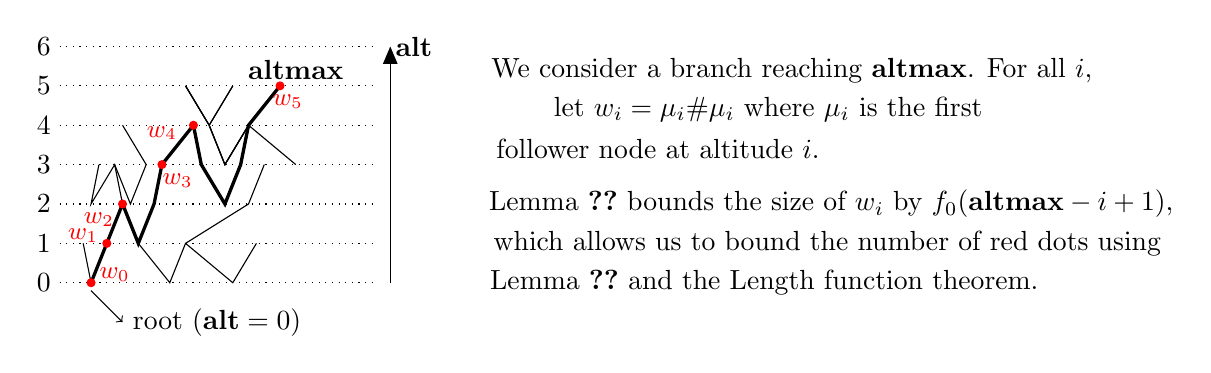
\begin{tikzpicture}
	
	\draw[dotted] (0,0) -- (4,0);
	\draw[dotted] (0,0.5) -- (4,0.5);
	\draw[dotted] (0,1) -- (4,1);
	\draw[dotted] (0,1.5) -- (4,1.5);
	\draw[dotted] (0,2) -- (4,2);
	\draw[dotted] (0,2.5) -- (4,2.5);
	\draw[dotted] (0,3) -- (4,3);
	
	\node at (-0.2,0) {$0$};
	\node at (-0.2,0.5) {$1$};
	\node at (-0.2,1) {$2$};
	\node at (-0.2,1.5) {$3$};
	\node at (-0.2,2) {$4$};
	\node at (-0.2,2.5) {$5$};
	\node at (-0.2,3) {$6$};
	
	\draw[very thick] (0.4,0) -- (0.6, 0.5) -- (0.8, 1) -- (1, 0.5) -- (1.2, 1) -- (1.3, 1.5) -- (1.7, 2) -- (1.8, 1.5) -- (2.1, 1) -- (2.3, 1.5) -- (2.4, 2) -- (2.8, 2.5);
	\draw (1, 0.5) -- (1.4, 0) -- (1.6, 0.5) -- (2.4, 1) -- (2.6, 1.5);
	\draw (1.6, 0.5) -- (2.2, 0) -- (2.5, 0.5);
	\draw (0.8, 1) -- (0.7, 1.5) -- (0.4, 1) -- (0.5, 1.5);
	\draw (0.7, 1.5) -- (0.9, 1) -- (1.1, 1.5) -- (0.8, 2);
	\draw (2.4, 2) -- (2.1, 1.5) -- (1.9, 2) -- (1.6, 2.5);
	\draw (2.4, 2) -- (2.1, 1.5) -- (1.9, 2) -- (1.6, 2.5);
	\draw (2.4, 2) -- (2.1, 1.5) -- (1.9, 2) -- (1.6, 2.5);
	\draw (1.9, 2) -- (2.2, 2.5);
	\draw (2.4, 2) -- (3, 1.5);
	\draw (1.9, 2) -- (2.2, 2.5);
	\draw (0.4, 0) -- (0.3, 0.5);
	
	\draw[->, >=triangle 45] (4.2, 0) -- (4.2, 3);
	
	
	\node (H) at (4.5, 3) {$\mathbf{alt}$};
	
	\draw[->] (0.4, -0.1) -- (0.8, -0.5);
	
	\node (R) at (2,-0.5) {root ($\mathbf{alt} =0$)};
	\node (AM) at (3,2.7) {$\altmax$};
	\draw[red, fill=red] (0.4, 0) circle (0.05);
	\draw[red, fill=red] (0.6, 0.5) circle (0.05);
	\draw[red, fill=red] (0.8, 1) circle (0.05);
	\draw[red, fill=red] (1.3, 1.5) circle (0.05);
	\draw[red, fill=red] (1.7, 2) circle (0.05);
	\draw[red, fill=red] (2.8, 2.5) circle (0.05);
	
	
	\node[red] at (0.7, 0.1) {\small $w_0$};
	\node[red] at (0.3, 0.6) {\small $w_1$};
	\node[red] at (0.5, 0.8) {\small $w_2$};
	\node[red] at (1.5, 1.3) {\small $w_3$};
	\node[red] at (1.3, 1.9) {\small $w_4$};
	\node[red] at (2.9, 2.3) {\small $w_5$};
	
	\node (txt) at (9.3, 2.7) {We consider a branch reaching $\altmax$. For all $i$,};
	\node (txt) at (9, 2.2) {let $w_i = \followlabelword{\node_i}\#\followlabelmessage{\node_i}$ where $\node_i$ is the first};
	\node (txt) at (7.6, 1.7) {"follower node" at altitude $i$.};
	
	\node (txt) at (9.8, 1) {Lemma~\ref{lem:bound-length-at-height-h} bounds the size of $w_i$ by $f_0(\altmax-i+1)$, };
	\node (txt) at (9.75, 0.5) {which allows us to bound the number of red dots using};
	\node (txt) at (8.95, 0) {Lemma~\ref{lem:shortening-branches} and the "Length function theorem".};
\end{tikzpicture}
	\caption{Illustration of the proof of Lemma~\ref{lem:bound-max-height}}.
	\label{fig:max-height-bound}
\end{figure}
\begin{restatable}{lemma}{lemBoundMaxHeight}
	\label{lem:bound-max-height}
	There exists a function $f_1$ of the class $\Ffunction{\omega^{\size{\messages}}}$ such that for all "protocol" $\prot$, for all "unfolding tree" $\tree$ of minimal size labeled by $\prot$ satisfying a "boss specification" $w$, the maximal altitude of a node of $\tree$ is bounded by $f_1(\size{\prot} + \size{w})$.
\end{restatable}
\begin{proof}
	Let $\tree$ be a "unfolding tree" of minimal size labeled by $\prot$ satisfying a "boss specification" $w$. Let $\altmax$ be the maximal altitude of a node in $\tree$. Let $\node_0$ the root of the tree, and  $\node_0, \ldots, \node_m$ a branch of the tree going from the root to a node $\node_m$ of altitude $\altmax$ (for all $i$, $\node_i$ is a child of $\node_{i-1}$).
	For all $a \in \nset{1}{\altmax}$, let $j_a$ be the minimal index such that $\altitude{\node_{j_a}} = a$. This index exists as $\altitude{\node_0} = 0$, $\altitude{\node_m} = \altmax$ and for all $i$, $\altitude{\node_{i}} \leq \altitude{\node_{i-1}}+1$.
	Furthermore, for every $a$, for every $j < j_a$, $\altitude{\node_j} < a$. 
	As a consequence, we have $j_1 < j_2 < \ldots < j_{\altmax}$. Moreover, $\node_{j_a}$ is necessarily a "follower node" as otherwise we would have $\altitude{\node_{j_a-1}} = a+1$ which contredicts minimality of $j_a$.
	
	We will bound $\altmax$ using Theorem~\ref{thm:lengthfcttheorem}. For simplicity, we will encode the $\followmessagespec$ part using a fresh character added to our alphabet (this is why we obtain a function in $\Ffunction{w^{\size{\messages}}}$ and not $\Ffunction{w^{\size{\messages}-1}}$; in fact, one could obtain the latter bound using Theorem 5.3. of~\cite{SchmitzS2011upperHigman}, but the proof would be more involved).

	Let $\# \notin \messages$ be a fresh letter, and let $N = \size{w} + \size{\prot}+1$. For all $i \in \nset{1}{\altmax}$ let $\node'_i = \node_{j_{\altmax - i+1}}$ and $w_i = \followlabelword{\node'_{i}} \# \followlabelmessage{\node'_{i}} \in (\messages \cup \set{\#})^*$.
	
	We claim that we cannot have $w_{i_1}\subword w_{i_2}$ for any  $i_1< i_2$.
	Suppose by contradiction that there exist such $i_1$ and $i_2$ with $i_1 < i_2$. Then we would have $\followlabelword{\node'_{i_1}} \subword \followlabelmessage{\node'_{i_2}}$ and $\followlabelmessage{\node'_{i_1}} = \followlabelword{\node'_{i_2}}$.
	Therefore, as $\node_{i_1}$ is a descendant of $\node_{i_2}$, by second case of Lemma~\ref{lem:shortening-branches} there would exist a "unfolding tree" of smaller size than $\tree$ satisfying $w$, contradicting the minimality of $\tree$.
	
	As a result, the sequence $(w_i)_{1\leq i \leq \altmax}$ is a "bad sequence" over the alphabet $\messages\cup\set{\#}$.
	Furthermore, by Lemma~\ref{lem:bound-length-at-height-h}, for all $i$, as $\altitude{\node'_{i}} = \altmax-i+1$, we have $\size{\followlabelword{\node_{j_a}}} \leq f_0(\size{\prot} + i)$ therefore $\size{w_i} \leq f_0^{(i)}(\size{\prot})$ (with $f_0^{(i)}$ denoting $f_0$ applied $i$ times).
	
	Because $f_0$ is primitive-recursive, we can apply Theorem~\ref{thm:lengthfcttheorem}: there exists a function $f_1' \in \Ffunction{\omega^{\size{\messages}}}$ such that the sequence $(w_i)_{i \in \nset{1}{\altmax}}$ is of length at most $f_1'(N)$. This prove that $\altmax \leq f_1'(N) = f_1'(\size{\prot} + \size{w} + 1)$. Letting $f_1 :n \mapsto f_1'(n+1)$ concludes the proof.
\end{proof}


The bound on the maximal altitude, along with Lemma~\ref{lem:bound-length-at-height-h}, gives us a bound on the size of the root. 
By using a similar argument as for the maximal altitude, we consider a branch reaching minimal altitude to obtain a "bad" sequence of "boss" nodes and apply the "Length function theorem" again to bound the minimal altitude.



\begin{restatable}{lemma}{lemBoundMinHeight}
	\label{lem:bound-min-height}
	There exists a function $f_2$ of the class $\Ffunction{\omega^{\size{\messages}+1}}$ such that for all "protocol" $\prot$, for all "unfolding tree" $\tree$ of minimal size labeled by $\prot$ satisfying a "boss specification" $w$, the absolute value of the minimal "altitude" of a node of $\tree$ is bounded by $f_2(\size{\prot} + \size{w})$.
\end{restatable}

\begin{proof}
	We proceed similarly as in the proof of Lemma~\ref{lem:bound-max-height}.
	
	Let $\tree$ be a "unfolding tree" of minimal size labeled by $\prot$ satisfying a "boss specification" $w$. Let $\altmin$ be the minimal altitude of a node in $\tree$. Let $\node_0, \ldots, \node_m$ be nodes of $\tree$ such that $\node_0$ is its root, $\altitude{\node_m} = \altmin$, and for all $i\in \nset{1}{m}$, $\node_i$ is a child of $\node_{i-1}$.
	For all $a \in \nset{\altmin}{0}$, let $j_a$ be the minimal index such that $\altitude{\node_{j_a}} = a$. This index exists as $\altitude{\node_0} = 0$, $\altitude{\node_m} = \altmin$ and for all $i$, $\altitude{\node_{i}} \geq \altitude{\node_{i-1}}-1$.
	Furthermore as $j_a$ is the minimal such index, we cannot have $\altitude{\node_j} \leq a$ for any $j < j_a$ as otherwise there would be a $j'$ such that $j' \leq j < j_a$ with $\altitude{\node_{j'}} = a$.
	
	As a consequence, we have $j_0 < j_1 < j_2 < \ldots < j_{|\altmin|}$. Moreover, $\node_{j_a}$ is necessarily a "boss node" for all $a<0$ as otherwise we would have $\altitude{\node_{j_a-1}} = a-1 \leq a$, and $\node_{j_0}$ is the root and therefore also a "boss node" as $\tree$ satisfies $w$.
	
	Let $N := \size{w} + \size{\prot}+1$. For all $i \in \nset{0}{|\altmin|}$ let $\node'_i = \node_{j_{-i}}$ and $w_i = \bosslabel{\node'_{i}} \in \messages^*$.
	
	We claim that we cannot have $w_{i_1}\subword w_{i_2}$ for any  $i_1< i_2$.
	Suppose by contradiction that there exist such $i_1$ and $i_2$ with $i_1 < i_2$. Then we would have $\bosslabel{\node'_{i_1}} \subword \bosslabel{\node'_{i_2}}$, hence, as $\node_{i_2}$ is a descendant of $\node_{i_1}$, by first case of Lemma~\ref{lem:shortening-branches} there would exist a "unfolding tree" of smaller size than $\tree$ satisfying $w$, contradicting the minimality of $\tree$.
	
	As a result, the sequence $(w_i)_{1\leq i \leq \altmax}$ is a "bad sequence" for the "subword order" over the alphabet $\messages\cup\set{\#}$.
	By Lemma~\ref{lem:bound-length-at-height-h}, for all $\node'_i$ we have $\size{\bosslabel{\node'_i}} \leq f_0(\size{\prot} + \altmax - \altitude{\node'_i}+1) = f_0(\size{\prot} + \altmax +i+1)$.
	By Lemma~\ref{lem:bound-max-height}, we have $\altmax \leq f_1(N)$ and thus $\size{\bosslabel{\node'_i}} \leq  f_0(N+f_1(N)+i)$. Let $g: k \geq 1 \mapsto f_0(k)$; clearly, for all $i$, $\size{w_i} \leq g^{(i)}(M)$ where $M := f_0(N + f_1(N)+1)$ (obviously, $f_0(k) > k+1$) and $g$ is primitive-recursive.
	
	We apply Theorem~\ref{thm:lengthfcttheorem} to obtain $h \in \Ffunction{\omega^{\size{\messages}}}$ such that $(w_i){1\leq i \leq \altmax}$ cannot have more than $h(M)$ elements, thus $|\altmin| \leq h(M)+1 = f_4(f_0(N+f_1(N)+1))$. By defining $f_2: n \mapsto f_4(f_0(n+f_1(n+1)+2))$, this means that $|\altmin| \leq f_2(\size{\prot} + \size{w})$. Moreover, $f_2$ is a function of $\Ffunction{\omega^{\size{\messages}+1}}$ as $f_0$, $f_1$ and $h$ are in $\Ffunction{\omega^{\size{\messages}}} \subseteq \Ffunction{\omega^{\size{\messages}+1}}$ and $\Ffunction{\omega^{\size{\messages}+1}}$ is closed by composition with functions of $\Ffunction{\omega^{\size{\messages}}}$.
\end{proof}

With the bounds on the maximal and minimal altitudes, Lemma~\ref{lem:bound-length-at-height-h} yields a bound on the size of all nodes in the tree.


\begin{lemma}
	\label{lem:bound-node-size}
	There exists a function $f_3$ of the class $\Ffunction{\omega^{\size{\messages}+1}}$ such that for all "protocol" $\prot$, for all "unfolding tree" $\tree$ of minimal size labeled by $\prot$ satisfying a "boss specification" $w$, for all node $\node$ of $\tree$,
	
		\begin{itemize}
		\item $\size{\localrunlabel{\node}} \leq f_3(\size{\prot}+ \size{w})$
			
		\item If $\node$ is a "boss node" then $\size{\bosslabel{\node}} \leq f_3(\size{\prot}+ \size{w})$.
		
		\item If $\node$ is a "follower node" then $\size{\followlabelword{\node}} \leq f_3(\size{\prot}+ \size{w})$.
	\end{itemize} 
\end{lemma}
\begin{proof}
	Using Lemmas~\ref{lem:bound-length-at-height-h}, \ref{lem:bound-max-height} and \ref{lem:bound-min-height}, we obtain that, for every node $\node$, the value $\altmax - \altitude{\node}$ is at most $f_1(\size{\prot} + \size{w}) + f_2(\size{\prot} + \size{w})$. We then apply Lemma~\ref{lem:bound-length-at-height-h} to bounds on $\localrunlabel{\node}$ and $\speclabel{\node}$ by $f_0(f_1(\size{\prot} + \size{w}) + f_2(\size{\prot} + \size{w})+1) \leq f_3(\size{\prot} + \size{w})$ where $f_3: n \mapsto f_0(f_1(n) + f_2(n)+1)$; $f_3$ is in $\Ffunction{\omega^{\size{\messages}+1}}$ as $\Ffunction{\omega^{\size{\messages}+1}}$ is closed by composition with elementary functions. 
\end{proof}

Finally, as we now have a bound on all nodes, we can easily bound the length of branches and the number of children of all nodes to get abound on the total size of the tree.

\PropBoundTreeSize*

	% There exists a function $f$ of the class $\Ffunction{\omega^{\size{\messages}+1}}$ such that for all "protocol" $\prot$, for all "unfolding tree" $\tree$ of minimal size labeled by $\prot$ satisfying a "boss specification" $w$, the size of $\tree$ is bounded by $f(\size{\prot} + \size{w})$.

\begin{proof}
	Recall that the size of $\tree$ is defined as the sum of the sizes of its nodes. 

	Thanks to Proposition~\ref{prop:trees-sound-complete}, $(\prot,q_f)$ is positive if and only if there exists a "coverability witness" for $(\prot,q_f)$.
	Let $\tree$ be a "coverability witness" of $(\prot,q_f)$, \emph{i.e.}, its root is a "boss node" whose local run covers $q_f$. Let $N = \size{\prot}+1$. Observe that one can encode the condition that this local run covers $q_f$ in the "boss specification" of the protocol (adding a special broadcast message only broadcast from $q_f$); in the following we will forget about the condition that the local run at the root covers $q_f$.
	
	We first bound the height of $\tree$ (\emph{i.e.}, the difference between its maximum and minimum "altitude"), then its arity (the maximal number of children of a node), which allows us to obtain a bound on the number of nodes. The sizes of the nodes will finally be bounded using the size of the height. 
	
	By Lemma~\ref{lem:bound-node-size}, for all "boss node" $\node$ in $\tree$ we have $\size{\bosslabel{\node}} \leq f_3(N)$.
	If a branch contains strictly more than $\sum_{i=0}^{f_3(N)}\size{\messages}^{i}$ "follower nodes", then there are two nodes in it with the same "boss" label, hence $\tree$ can be reduced and still satisfy $w$, contradicting the minimality of $\tree$.

	Similarly, by Lemma~\ref{lem:bound-node-size}, for all "follower node" $\node$ in $\tree$ we have $\size{\followlabelword{\node}} \leq f_3(N)$.
	If a branch contains strictly more than $\size{\messages} \sum_{i=0}^{f_3(N)}\size{\messages}^{i}$ "follower nodes", then there are two nodes in it with the same "follower" label, hence $\tree$ can be reduced and still satisfy $w$, contradicting the minimality of $\tree$.
	
	As a result, each branch of $\tree$ contains at most $(\size{\messages}+1) \sum_{i=0}^{f_3(N)}\size{\messages}^{i}$ nodes. We simplify this expression: let $H: n \mapsto n (f_3(n)+1) n^{f_3(n)+1}$, each branch of $\tree$ has less than $H(N)$ nodes.
	
	Furthermore, by Lemma~\ref{lem:bound-successor-height}, each node has at most $\size{\messages}r$ "follower" children. Moreover, if a node $\node$ has more than $f_3(N)$ "boss" children, then one of them can be removed as at most $f_3(N)$ non-initial values appear in $\localrunlabel{\node}$; this would contradict the minimality of $\tree$.	
	As a consequence, each node in $\tree$ has at most $f_3(N) + \size{\messages}(r+1)$ children.

	% Let $\node$ be a node of $\tree$, let $V$ be the set of non-initial values appearing in $\localrunlabel{\node}$ apart from $\valuelabel{\node}$.
	% By condition~\ref{item:condition1_non_initial_value}, for each $v' \in V$, $\node$ has a "boss" child $\node_{v'}$ such that $\vinput{v'}{\localrunlabel{\node}} \subword \bosslabel{\node_{v'}}$.
	% We simply observe that $\size{V} \leq \size{\localrunlabel{\node}}$ as every non-initial value needs to be received at some point in $\localrunlabel{\node}$. We also note that all other "boss" children of $\node$ can be removed, and the resulting tree still satisfies $w$ and is still a "unfolding tree". By minimality of $\tree$, this means that $\mu$ has at most $\size{\localrunlabel{\node}}$ "boss" children, hence at most $f_3(N)$ by Lemma~\ref{lem:bound-node-size}.
	
	By combining the bounds on the size of branches and the arity of nodes, we obtain that $\tree$ has at most $\sum_{h=0}^{H} (f_3(N) + \size{\messages}r)^h$ nodes. Let $G: n \mapsto (H(n)+1)(f_3(n) + n^2)^{H(n)}$. The total number of nodes in $\tree$ is at most $G(N)$.
	
	Finally, we obtain a bound on the size of $\tree$ by taking the product of the bounds on the number of nodes and on the size of each node label: 
	\[ \size{\tree} \leq  G(N) (2 f_3(N)+1)\]
	
	Let $f: n \mapsto  G(n+1) (2 f_3(n+1) +1)$; using the fact that $n \leq f_3(n)$, we can bound $f_4$ by the composition of an elementary fonction with $f_3$, hence as $f_3 \in \Ffunction{\omega^{\messages}}$ and $\Ffunction{\omega^{\messages}}$ is closed by composition with elementary functions, we have that $f_4 \in \Ffunction{\omega^{\messages}}$.
	Overall, we have shown that the size of a minimal "coverability witness" for $(\prot,q_f)$ is bounded by $f(\size{\prot})$ with $f \in \Ffunction{\omega^{\size{\messages}}}$.
\end{proof}


%	\section{Proof of Proposition~\ref{prop:target-undec}}

\propTargetUndecidable*

\begin{proof}
	We present a reduction of the "halting problem" for "Minsky machines" to "target reachability problem" for BNRA.
	
	A "Minsky Machine" is a tuple $M= (\Loc, \Delta, \Cpt, \ell_0, \ell_f)$ where $\Loc$ is a finite set of locations, $\Cpt = \{\cpt_1, \cpt_2\}$ is a set of two counters, $\Delta \subseteq \Loc \times (\{\dec{\cpt}\}_{\cpt \in \Cpt} \cup \{\inc{\cpt}\}_{\cpt \in \Cpt} \cup \{\testz{\cpt}\}_{\cpt \in \Cpt} ) \times \Loc$ is a finite set of transitions, $\ell_0 \in \Loc$ is an initial location, and $\ell_f \in \Loc$ is a final location. A \emph{configuration} of a Minsky machine is a tuple $(\ell, v_1, v_2) \in \Loc \times \nats \times \nats$ where $v_1$ (resp. $v_2$) stands for the value of the counter $\cpt_1$ (resp. $\cpt_2$). The initial configuration is the configuration $(\ell_0, 0, 0)$.
	For two configurations $(\ell, v_1, v_2)$ and  $(\ell', v'_1, v'_2)$, we note $(\ell, v_1, v_2) \stepMM{} (\ell', v'_1, v'_2)$ if $\exists \delta \in \Delta$ such that one of the following condition holds:
	\begin{itemize}
		\item $\delta = (\ell, \inc{\cpt_i}, \ell')$ and $v'_i = v_i+1$, $v_{3-i} = v'_{3-i}$;
		\item $\delta = (\ell, \dec{\cpt_i}, \ell')$ and $v'_i = v_i-1$, $v_{3-i} = v'_{3-i}$;
		\item $\delta = (\ell, \testz{\cpt_i}, \ell')$ and $v'_i = v_i = 0$, $v_{3-i} = v'_{3-i}$.
	\end{itemize}
	%	We will note $\stepMM{}$ for $\bigcup_{\delta \in \Delta} \stepMM{\delta}$. 
	An execution of the machine is a sequence $(\ell_1, v_1^1, v_2^1) \stepMM{} (\ell_2, v_1^2, v_2^2) \stepMM{} \dots \stepMM{} (\ell_k, v_1^k, v_2^k)$. We say that an execution is initial if it starts with the initial configuration.
	The "halting problem" asks whether there exists an initial execution ending with a configuration $(\ell_f, v_1, v_2)$ where $v_1$, $v_2$ are any values in $\nats$. This problem is well-known to be undecidable.
	%\luin{to make the proof easier, one might require that there is no two transitions doing the same operation from a same location, this does not change the undecidability}
	
	
	%	\begin{figure}
		%		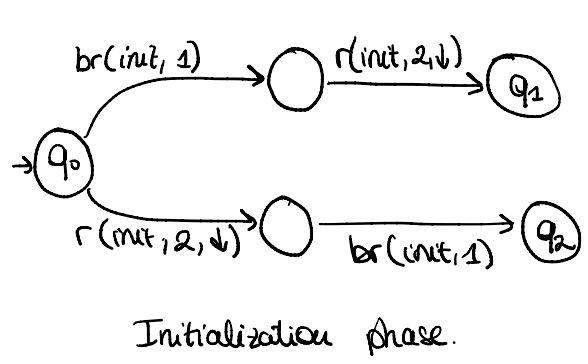
\includegraphics[scale = 0.25]{Figures/init.png}
		%		\caption{init}\label{fig:target:init}
		%	\end{figure}
	
	\begin{figure}
		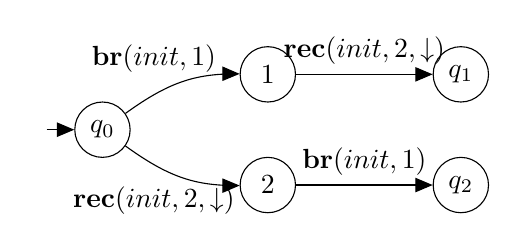
\begin{tikzpicture}[xscale=0.5,AUT style,node distance=2.1cm,auto,>= triangle
	45]
	\tikzstyle{initial}= [initial by arrow,initial text=,initial
	distance=.7cm]
	%	\tikzstyle{accepting}= [accepting by arrow,accepting text=,accepting
	%	distance=.7cm,accepting where =right]
	
	\node[state,initial, minimum width=0.1pt] (0) at (0,0) {$q_0$};
	\node[state] [right of=0, yshift=20] (x) {1};
	\node[state] [right of=0, yshift=-20] (y) {2};
	\node[state] [right of=x, xshift=10] (1) {$q_1$};
	\node[state] [right of=y, xshift=10] (2) {$q_2$};
	
	\path[->, bend left=10] 	
	(0) edge node[above, xshift=-10] {$\br{init}{1}$} (x)
	;
	\path[->, bend right=10] 	
	(0) edge node[below, xshift=-10] {$\rec{init}{2}{\enregact}$} (y)
	;
	\path[->] 	
	(x) edge node {$\rec{init}{2}{\enregact}$} (1)
	(y) edge node {$\br{init}{1}$} (2)
	;
\end{tikzpicture}
		\caption{init}\label{fig:target-init}
	\end{figure}
	
	%	\begin{figure}
		%		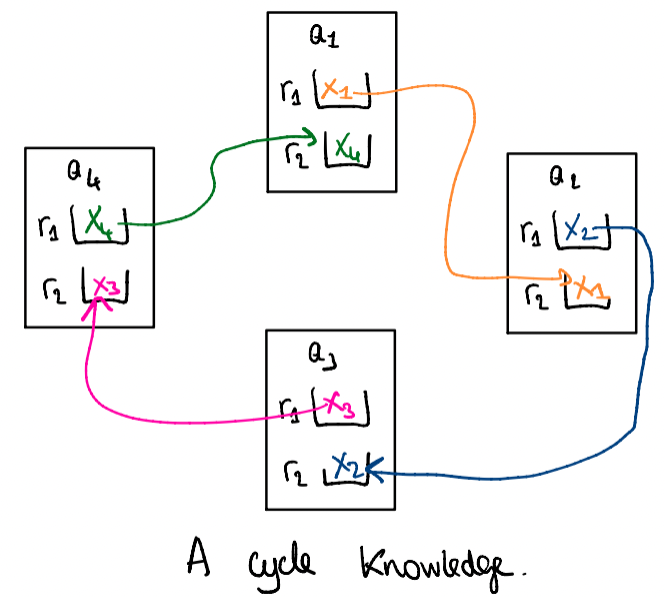
\includegraphics[scale = 0.3]{Figures/cycle-knowledge.png}
		%		\caption{ck}\label{fig:target:cycle-knowledge}
		%	\end{figure}
	
	
	
	
	\begin{figure}
		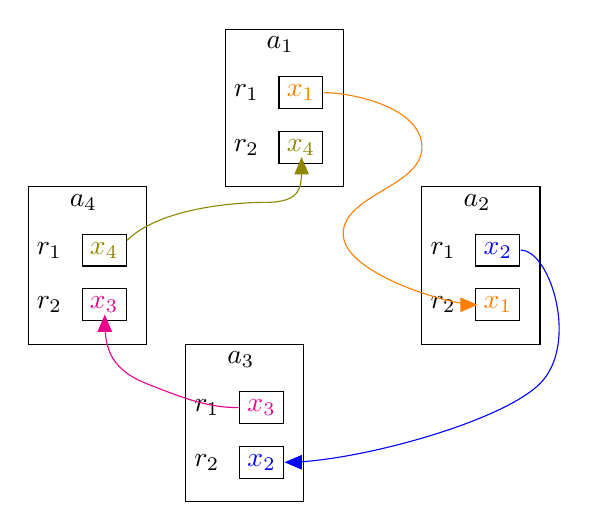
\begin{tikzpicture}[AUT style,node distance=2.1cm,auto,>= triangle
	45]
	\tikzstyle{initial}= [initial by arrow,initial text=,initial
	distance=.7cm]
	%	\tikzstyle{accepting}= [accepting by arrow,accepting text=,accepting
	%	distance=.7cm,accepting where =right]
	
	
	\draw (0,0) rectangle (1.5,2);
	\draw (3,2) rectangle (4.5,4);
	\draw (-2,2) rectangle (-0.5,4);
	\draw (0.5,4) rectangle (2,6);
	
	\node (Q1) at (1.2,5.8) {$a_1$};
	\node (Q2) at (3.7,3.8) {$a_2$};
	\node (Q3) at (0.7,1.8) {$a_3$};
	\node (Q4) at (-1.3,3.8) {$a_4$};
	
	\node (Q1R1) [below left of=Q1, xshift=30, yshift=25] {$r_1$};
	\node (Q2R1) [below left of=Q2, xshift=30, yshift=25] {$r_1$};
	\node (Q3R1) [below left of=Q3, xshift=30, yshift=25] {$r_1$};
	\node (Q4R1) [below left of=Q4, xshift=30, yshift=25] {$r_1$};
	
	\node (Q1R2) [below of=Q1R1, yshift=40] {$r_2$};
	\node (Q2R2) [below of=Q2R1, yshift=40] {$r_2$};
	\node (Q3R2) [below of=Q3R1, yshift=40] {$r_2$};
	\node (Q4R2) [below of=Q4R1, yshift=40] {$r_2$};
	
	\node[draw,inner sep=1mm] (Q1X1) [right of=Q1R1, xshift=-40] {\color{orange} $x_1$};
	\node[draw,inner sep=1mm] (Q2X2) [right of=Q2R1, xshift=-40] {\color{blue} $x_2$};
	\node[draw,inner sep=1mm] (Q3X3) [right of=Q3R1, xshift=-40] {\color{magenta}$x_3$};
	\node[draw,inner sep=1mm] (Q4X4) [right of=Q4R1, xshift=-40] {\color{olive} $x_4$};
	
	\node[draw,inner sep=1mm] (Q1X4) [below of=Q1X1, yshift=40] {\color{olive} $x_4$};
	\node[draw,inner sep=1mm] (Q2X1) [below of=Q2X2, yshift=40] {\color{orange} $x_1$};
	\node[draw,inner sep=1mm] (Q3X2) [below of=Q3X3, yshift=40] {\color{blue}$x_2$};
	\node[draw,inner sep=1mm] (Q4X3) [below of=Q4X4, yshift=40] {\color{magenta}$x_3$};
	
	\node (A11) [right of=Q1X1, xshift=-55] {};
	\node (A22) [right of=Q2X2, xshift=-55] {};
	\node (A44) [right of=Q4X4, xshift=-55] {};
	\node (A32) [right of=Q3X2, xshift=-55] {};
	
	\node (A33) [left of=Q3X3, xshift=55] {};
	\node (A14) [left of=Q1X4, xshift=60] {};
	\node (A21) [left of=Q2X1, xshift=56] {};
	\node (A43) [left of=Q4X3, xshift=60] {};
	
	\draw[color=orange] (A11) ..controls +(0.5,0) and +(0,0.5).. (3,4.5); % arc 1
	\draw[color=orange] (3,4.5) ..controls +(0,-0.5) and +(0,0.5).. (2,3.4); % arc 2
	\draw[color=orange, ->] (2,3.4) ..controls +(0,-0.5) and +(-0.5,0).. (A21); % arc 3
	
	
	\draw[color=blue] (A22) ..controls +(0.5,0) and +(0.5,0.5).. (4.5,1.5); % arc 1
	\draw[color=blue, ->] (4.5,1.5) ..controls +(-0.5,-0.5) and +(1,0).. (A32); % arc 2
	
	
	\draw[color=magenta] (A33) ..controls +(-0.5,0) and +(0.5,-0.2).. (-0.5,1.5); % arc 1
	\draw[color=magenta, ->] (-0.5,1.5) ..controls +(-0.5,0.2) and +(0,-0.5).. (A43); % arc 2
	
	\draw[color=olive] (A44) ..controls +(0.5,0.5) and +(-0.5,0).. (1,3.8); % arc 1
	\draw[color=olive, ->] (1,3.8) ..controls +(0.5,0) and +(0,-0.5).. (A14); % arc 2
\end{tikzpicture}
		\caption{Illustration of a cycle of knowledge of 4 agents. Each box represents an agent along with tis register's values.}\label{fig:target-cycle-knowledge}
	\end{figure}
	
	Fix a "Minsky Machine" $M= (\Loc, \Delta, \Cpt, \ell_0, \ell_f)$. The simulation will go as follows: 
	\begin{itemize}
		\item each agent will have two registers: one with its identity, which it will broadcast, and another in which it will store the value of a \emph{predecessor} process. To do so, in an initialization phase, each process makes one of the following choice: (i) it starts by broadcasting its first register value and then wait to receive (and store in its second register) a value, (ii) it waits first for a value to store in its second register and then broadcasts its first register value. This initialization part will appear in the protocol as displayed in \cref{fig:target-init}. Note that, after the initialization phase (once all processes reached $q_1$ and $q_2$), there is necessary a \emph{cycle of knowledge} in the reached configuration. A cycle of knowledge in a configuration $\config$ is a subset of agents $\{a_1, \dots a_k\}$ such that for all $1 \leq i < j \leq k$, $\data{\config}(a_i)(1) \ne \data{\config}(a_j)(1)$, for all $2 \leq i \leq k$, $\data{\config}(a_i)(2) = \data{\config}(a_{i-1})(1)$ and $\data{\config}(a_1)(2) = \data{\config}(a_{k})(1)$ (see \cref{fig:target-cycle-knowledge}). Indeed, consider the function wich associates to each agent $a$, an agent $a'$ such that $\data{\config}(a)(2) = \data{\config}(a')(1)$. This function is total as $\gamma$ is such that all agents reached states $q_1$ or $q_2$. By the pigeonhole principle, there exists a cycle of knowledge.
		
		%		configurations can be decomposed as an union of \emph{cycles of knowledge} (\cref{fig:target:cycle-knowledge}). A cycle of knowledge in a configuration $\config$ is a subset of agents $\{a_1, \dots a_k\}$ such that for all $1 \leq i < j \leq k$, $\data{\config}(a_i)(1) \ne \data{\config}(a_j)(1)$, for all $2 \leq i \leq k$, $\data{\config}(a_i)(2) = \data{\config}(a_{i-1})(1)$ and $\data{\config}(a_1)(2) = \data{\config}(a_{k})(1)$. Indeed, there exists an injective function from $\agentsof{\gamma}$ into itself associating to each agent $a_1$, any agent $a_2$ such that $\data{\config}(a_2)(2) = \data{\config}(a_1)(1)$. By the pigeonhole principle, the function is a union of cycles. \cortoin{Il peut aussi y avoir des agents sans successeurs, donc des arbres de flèches qui partent d'un cycle mais ne font pas partie d'un cycle.}
		
		From now, an agent will broadcast only its first register value (along with some messages) and shall only receive messages sent with its second register value. In other words, every reception transition after the initialisation phase is of the form $\rec{m}{2}{=}$ for some $m \in \messages$ and every broadcast transition after the initialisation  phase is of the form $\br{m}{1}$ for some $m \in \messages$;
		
		\item From now, we focus on one cycle of knowledge (any of them suits to simulate the machine). once it is done, the agents which made the first choice (i) during the initialization phase will simulate a machine execution. We shall name this type of agents \emph{leader} agents. Note that there is at least one such agent in the cycle of knowledge, otherwise, no agent sent its value first and the cycle cannot be created. 
		The other agents of the cycle will simulate the counters' values, each agent chooses one of the two counters to simulate, it is either on the zero-state or in the one-state of the appropriate counter. Given a configuration of the protocol, we associate a machine configuration as follows: the location machine is the state of any leader agent of the cycle, and the value of counter 1 (resp. 2) is the number of agents on the one-state of the counter.
		
		\item At the beginning, leader agents are location $\ell_0$ and other agents are all on one of the zero-states. Assume for now there is only one leader agent on the cycle, to a transition $(\ell, \inc{\cpt_1}, \ell')$, the leader agent sends message $\mathtt{inc_1}$ and waits to receive an acknowledgment message $\mathtt{Ainc_1}$ from its predecessor, then it moves to the location $\ell'$. The message $\mathtt{inc_1}$ is received by its successor on the cycle (and only by this agent). When an agent on the cycle receives a message from its predecessor, either it repeats it, either its changes its state (in this case, one agent on the zero-state of counter 1 shall move to the one-state of counter 1) and sends a acknowledgment message that the operation has been made (in this case $\mathtt{Ainc_1}$). If an agent receives an acknowledgment message, it only forwards it to its successor. This way, when the leader receives the acknowledgment message, it knows that one process (and only one) moved to the one-state of counter 1. Note that if one message is lost the run stops. Note as well that if no agent changes state, the run stops as well because a message will be lost. Decrements transitions are simulated in an analogous manner.
		
		\item When it comes to reduce halting problem of Minsky Machines, usually the tricky part is to simulate test to 0 of counters. Here, once we have this cycle of knowledge structure, it is quite simple: when the leader wants to simulate a transition $(\ell, \testz{\cpt_1}, \ell')$, it sends a message $\mathtt{test_1}$ to its successor and waits to receive the \emph{same} message from its predecessor before changing its state to $\ell'$. When an agent receives the message from its predecessor, if it is \emph{not} on the one-state of counter 1, it forwards it to its successor, otherwise, it reaches a deadlock state in which it can do anything anymore. It blocks the run.
		
		\item once the leader agent reaches $\ell_f$, it sends the message $\mathtt{end}$ to its successor, when an agent receives the message $\mathtt{end}$, it reaches $\ell_f$ and forwards it to its successor.
		
		\item If there are two agents (or more) in the cycle of knowledge, they should all simulate the same machine execution. All agents in between two leaders will simulate counters' values of one execution, and if two agents make different choices, it will block the run of the protocol. \lu{to explain better...}
	\end{itemize}
\end{proof}
%	
\section{Proofs of section \ref{sec:cover-1BNRA}}
\luin{Plan : 1) diseq test, 2) Completeness, 3) Soundness, 4) conclusion (abstraction sound and complete, NP hardness, NP-complete)}

\label{app:cover-one-reg}
\subsection{Removing disequality tests}
\label{sec:one-diseq-tests}

\lemRemoveDiseq*

\ifproofs
\begin{proof}
	First, if $(\prot, q_f)$ is positive then so is $(\tilde{\prot}, q_f)$, as one can easily lift any "run" in $\prot$ to an equivalent "run" in $\tilde{\prot}$ (transitions are less guarded  in $\tilde{\prot}$ that in $\prot$). 
	
	Suppose now that $(\tilde{\prot}, q_f)$ is a positive instance of the "coverability problem". There exists a "run" $\tilde{\run}: \tilde{\config}_0 \step{*} \tilde{\config}$ in $\tilde{\prot}$ that covers $q_f$. We prove by induction on the length of $\tilde{\run}$ that there exists a "run" $\run$ reaching a configuration $\config$ such that $\tilde{\config} \lessthan \config$ (Remark~\ref{rem:bigger_config_query} then allows us to conclude). 
	
	If $\config = \config_0$ then $\run = \tilde{\run}$ suffices. Suppose that $\tilde{\run}$ has length $k \geq 1$, and that the result if true for "runs" of length $k-1$. Decompose $\tilde{\run}$ into $\tilde{\run_{k-1}}: \tilde{\config_0} \step{*} \tilde{\config_{k-1}}$ of length $k-1$ and a final step $\tilde{\config_{k-1}} \step{} \tilde{\config_k}$. 
	By induction hypothesis, there exists $\run_{k-1}: \config_0 \step{*} \config_{k-1}$ such that $\tilde{\config_{k-1}} \lessthan \config_{k-1}$: there exists an injective function $\pi : \tilde{\agents} \rightarrow \agents$
	such that, for all $a \in \tilde{\agents}$, $\tilde{\config_{k-1}}(a) = \config_{k-1}(\pi(a))$, where $\tilde{\agents} := \agentsof{\tilde{\run}}$ and $\agents := \agentsof{\run}$. If $\tilde{\config_{k-1}} \step{} \tilde{\config_k}$ involves no reception transition from $\tilde{\prot}$ whose corresponding transition in $\prot$ has action $\quotemarks{\diseqtestact}$, then we directly lift this step into a step appended at the end of $\run_{k-1}$ (making $\pi(a)$ take a transition whenever $a$ does so in $\tilde{\config_{k-1}} \step{} \tilde{\config_k}$). Otherwise, write $\tilde{\agents}_{\diseqtestact}$ the subset of $\tilde{\agents}$ corresponding to agents taking in $\tilde{\config_{k-1}} \step{} \tilde{\config_k}$ a reception transition from $\tilde{\prot}$ whose corresponding transition in $\prot$ has action $\quotemarks{\diseqtestact}$ . Write $(q, \brone{m}, q') \in \transitions$ the broadcast transition used in this step.  Using the copycat principle, we add to $\config_{k-1}$ a fresh agent $a_{\mathsf{new}}$ with state $q$ and a register value that does not appear in $\config_{k-1}$. 
	We first mimic this broadcast step at the end of $\run_{k-1}$, making any agent $\pi(a) \in \pi(\tilde{\agents} \setminus \tilde{\agents}_{\diseqtestact})$ take the transition that $a$ takes in $\tilde{\config_{k-1}} \step{} \tilde{\config_k}$. We then add a new step where $a_{\mathsf{new}}$ broadcasts using transition $(q, \brone{m}, q')$, and every agent $\pi(a) \in \pi(\tilde{\agents}_{\diseqtestact})$ takes the transition corresponding to the transition taken by $a$ in $\tilde{\config_{k-1}} \step{} \tilde{\config_k}$. Such a transition is a reception with action $\quotemarks{\diseqtestact}$ in $\prot$; however, because $a_{\mathsf{new}}$ does not share its register value with any process from $\tilde{\agents}$, all disequality conditions are satisfied and this step is valid. In this end, every agent $\pi(a) \in \pi(\tilde{\agents})$ has taken the transition in $\prot$ corresponding to the one $a$ took in $\tilde{\prot}$ in step $\tilde{\config_{k-1}} \step{} \tilde{\config_k}$, hence the configuration $\config_k$ reached by the constructed run is such that $\tilde{\config_k} \lessthan \config_k$. 
\end{proof}
\fi

\subsection{Completeness}
\label{one-completeness}

This subsection is devoted to proving Lemma~\ref{lem:abstraction_complete}.

\begin{lemma}
	\label{lem:abstraction_complete}
	If $\run$ is a (concrete) "run" and $\aval \in \valsof{\run}$, then $\aconfiginit \step{*} \absproj{\aval}{\run}$. 
\end{lemma}


% The following lemma shall later be useful:
% \begin{lemma}
	% \label{lem:adding_states_in_covset}
	% If $\aconfig = (\covset, \gang), \aconfig' = (\covset', \gang') \in \allaconfigs$ are such that $\aconfig \step{*} \aconfig'$ then $\covset \subseteq \covset'$ and, for all $T \subseteq Q$, $(\covset \cup T, \gang) \step{*} (\covset' \cup T, \gang')$. 
	% \end{lemma}
% \begin{proof}
	% To prove the first statement, in suffices to observe that, in a step of the abstract semantics, the set $\covset$ may not decrease.
	% To prove the second statement, it suffices to notice in the abstract semantics that a larger $\covset$ may never hinder a step. 
	% \end{proof}

\begin{lemma}
	\label{lem:proof_completeness_covset_constant}
	For all "runs" $\run: \config_0 \step{*} \config$ and $\aval \in \valsof{\run}$, $(\statesin{\run}, q_0, \emptyset) \step{*} \absproj{\aval}{\run}$. 
\end{lemma}

\ifproofs
\begin{proof}
	Let $\covset := \statesin{\run}$ and $\agents = \agentsof{\run}$.
	
	Thanks to Remark~\ref{rem:run_no_new_register_values},  $\aval$ appears in $\config_0$; let $a_0$ be the (unique) agent such that $\data{\config_0}(a_0) = \aval$. We write $\run : \config_0 \step{} \config_1 \step{} \dots \step{} \config_k = \config$. For every $i \leq k$, let $\run_i : \config_0 \step{*} \config_i$ be the prefix of $\run$ of length $i$, and write $\aconfig^i := (\covset, \gangof{\aval}{\run_i})$. Note that $\gangof{\aval}{\run_0} = (q_0, \emptyset)$ hence $\aconfig^0 = (\covset, q_0, \emptyset)$. Also, we write $(\covset, \boss_i, \clique_i) := \aconfig^i$.
	
	We prove by induction on $i$ that $\aconfig^0 \step{*} \aconfig^i$.
	The statement is trivially true for $i =0$. 
	
	Suppose now that $(\covset, \emptyset, \noboss) \step{*} \aconfig^i$. 
	If suffices to prove that $\aconfig^i \step{} \aconfig^{i+1}$. First of all we clearly have, by definition, $K_{i+1} \subseteq S$ and $\boss_{i+1}\in S\cup\set{\noboss}$. We consider the last step of $\run_{i+1}$, which is referred to under the name $s_{i+1}$ in what follows; $s_{i+1}: \config_i \step{} \config_{i+1}$. Let $\agentbr$ the agent making the broadcast transition in $s_{i+1}$ and $A_{\recsymb}$ the set of agents receiving this broadcast in $s_{i+1}$. Let $(\statebr, \brone{\amessage}, \statebr') \in \transitions$ denote the transition taken by $\agentbr$ in $s_{i+1}$.
	
	We now make the following case distinction to determine the type of the abstract step $\aconfig^i \step{} \aconfig^{i+1}$:
	\begin{enumerate}
		\item\label{proof_completeness:case_broadcast_clique} if $\data{\config_{i}}(\agentbr) = \aval$ but there exists $j<i$ such that $\data{\config_{j}}(\agentbr) \ne \aval$ then it is a ``broadcast from clique'',
		\item\label{proof_completeness:case_broadcast_boss} if, for all $j \leq i$, $\data{\config_j}(\agentbr) = \aval$ then it is a ``broadcast from boss'',
		\item\label{proof_completeness:case_external_broadcast} otherwise it is an ``external broadcast''. 
	\end{enumerate}
	Note that $\agentbr$ may not change its register value in $s_{i+1}$ hence $\data{\config_i}(\agentbr) = \data{\config_{i+1}}(\agentbr)$. 
	
	Let $\agentboss$ the agent such that $\data{\config_0}(\agentboss) = \aval$. In case~\ref{proof_completeness:case_broadcast_boss}, $\agentboss = \agentbr$; in the other two cases, $\agentboss \ne \agentbr$. 
	
	We now prove the other conditions:
	\begin{enumerate}[i]
		\item In case~\ref{proof_completeness:case_broadcast_clique}, since $\agentbr$ has value $\aval$ in $\config_i$ and $\config_{i+1}$ but not in every $\config_j$ for $j \leq i$, we directly have $\statebr \in \clique_i$ and $\statebr' \in \clique_{i+1}$. In case~\ref{proof_completeness:case_broadcast_boss}, it suffices to note that $\boss_i = \st{\config}(\agentbr)$ and $\boss_{i+1} = \st{\config_{i+1}}(\agentbr)$. In case~\ref{proof_completeness:case_external_broadcast}, it suffices to note that $\statebr, \statebr' \in \covset$ as both states appear in $\run$.
		\item In case~\ref{proof_completeness:case_broadcast_boss}, this condition is automatically satisfied. In the other two cases, we look at what $\agentboss$ does in $s_{i+1}$. If it remains idle then we have $\boss_i = \boss_{i+1}$. Otherwise it takes a reception transition as $\agentbr \ne \agentboss$. 
		In case~\ref{proof_completeness:case_external_broadcast}, this reception may not have action $\quotemarks{\eqtestact}$ as the broadcast is from an agent with register value that is not $\aval$ ($\data{\config_i}(\agentbr) \ne \aval$ by hypothesis). For the same reason, if this reception has action $\quotemarks{\enregact}$ then $\boss_{i+1}= \noboss$. If this reception has action $\quotemarks{\dummyact}$ and $\boss_i \ne \noboss$ then $\boss_{i+1} \ne \noboss$ as $\agentboss$ keeps value $\aval$.
		\item We have $\clique_i \subseteq \clique_{i+1}$ because $\run_{i}$ is a prefix of $\run_{i+1}$; also, in case~\ref{proof_completeness:case_broadcast_clique}, $\statebr' \in \clique_{i+1}$ because of $\agentbr$. Let $q' \in \clique_{i+1} \setminus \clique_i$ with, in case~\ref{proof_completeness:case_broadcast_clique}, $q' \ne \statebr'$. There exist $q\in \covset$ and an agent $a$ that takes a reception transition $(q, \rec{\amessage}{\anact}, q')$ in $s_{i+1}$ and has value $\aval$ in $\config_{i+1}$. In cases~\ref{proof_completeness:case_broadcast_clique} and \ref{proof_completeness:case_broadcast_boss}, the broadcast has value $\aval$ hence if $\anact = \quotemarks{\eqtestact}$ or $\quotemarks{\dummyact}$ then $a$ has value $\aval$ in $\config_i$ and $q \in \clique_i$. In case~\ref{proof_completeness:case_external_broadcast}, the broadcast has value $\ne \aval$ hence $a$ may have value $\aval$ in $\config_{i+1}$ only when $\anact = \quotemarks{\dummyact}$ and $a$ had value $\aval$ in $\config_i$, which implies $q \in \clique_i$. 
		\item It suffices to note that the first components of $\aconfig^i$ and $\aconfig^{i+1}$ are equal to $\covset$ and $\statebr' \in \covset$, and $\boss_{i+1} \in \covset \cup \set{\bot}$. 
	\end{enumerate}
	
	Overall, we have proven that $\aconfig^i \step{} \aconfig^{i+1}$, which concludes the induction step. Appyling the result with $i = k$ proves Lemma~\ref{lem:proof_completeness_covset_constant}. 
	
\end{proof}
\fi

\ifproofs
We may now prove Lemma~\ref{lem:abstraction_complete}. 

\begin{proof}[Proof of Lemma~\ref{lem:abstraction_complete}]
	Let $\run$ a run.
	We proceed by induction on the size of the set $\statesin{\run}$. 
	First, if $\statesin{\run}$ is of size $1$ then $\statesin{\run} = \set{q_0}$. Applying Lemma~\ref{lem:proof_completeness_covset_constant} directly gives $\aconfiginit = (\set{q_0}, q_0, \noboss) \step{*} \absproj{\aval}{\run}$.
	
	
	Suppose now that the statement is true for any $\run$ such that $\statesin{\run}$ is of size $k$, and suppose that we have a run $\run$ such that $\statesin{\run}$ is of size $k+1$. Let $\aval \in \valsof{\run}$. Let $\run_p: \config_0 \step{*}\config_p$ the longest suffix of $\run$ such that $\statesin{\run} \ne \statesin{\run_p}$. By induction hypothesis, we know that for all $\aval \in \valsof{\run}$, $\aconfiginit \step{*} \absproj{\aval}{\run_p}$. Write $s$ the step immediatly after $\run_p$ in $\run$. By maximality of $\run_p$, $\run_p s$ covers all states in $\statesin{\run} \setminus \statesin{\run_p}$. 
	
	Write $\agentbr$ the agent broadcasting in $s$, $(\statebr, \brone{\amessage}, \statebr')$ the corresponding transition and $\avalbr$ the broadcast value. By induction hypothesis applied to $\run_p$ and $\avalbr$, $\aconfiginit \step{*} \absproj{\avalbr}{\run_p}$. Applying Lemma~\ref{lem:proof_completeness_covset_constant} on $\run$ and $\aval$ gives that $(\statesin{\run}, q_0, \emptyset) \step{*} \absproj{\aval}{\run}$. Therefore, it remains to prove that $\absproj{\aval}{\run_p} \step{*} (\statesin{\run}, q_0, \emptyset)$. It suffices to prove that there exists $\boss, \clique$ such that $\absproj{\avalbr}{\run_p} \step{} (\statesin{\run}, \boss,\clique)$, a "gang reset" allowing us to then reach $(\statesin{\run}, q_0, \emptyset)$. In other words, we prove that, from $\absproj{\avalbr}{\run_p}$, one may cover all states in $\statesin{\run}$ in just one abstract step.
	
	We aim at proving that $\absproj{\avalbr}{\run_p} \step{} (\statesin{\run}, \boss,\clique)$ for well-chosen $\boss$ and $\clique$.
	Just like in the proof of Lemma~\ref{lem:proof_completeness_covset_constant}, we make a case disjunction to prove that the broadcast in $s$ may be mimicked in the abstraction from $\absproj{\avalbr}{\run_p}$. The type obtained is either a "broadcast from clique" or a "broadcast from boss", because by hypothesis the agent broadcasting has value $\avalbr$ and therefore its state before the broadcast is either the boss or in the clique in $\absproj{\avalbr}{\run_p}$. 
	
	Because we may choose $\boss$ and $\clique$ freely, the only challenging condition is \ref{item:broadcast_from_clique_covset}.
	Let $q' \in \statesin{\run} \setminus \statesin{\run_p}$, $q' \ne \statebr'$. 
	There exists an agent $a$ that takes a reception transition $(q,\recone{m}{\anact},q')$ in $s$. 
	If $\anact = \quotemarks{\eqtestact}$, then agent $a$ has value $\avalbr$ at the end of $\run_p$ hence $q$ is in the clique of $\absproj{\avalbr}{\run_p}$ and condition \ref{item:broadcast_from_clique_covset} is satisfied. Otherwise, one has $q \in \statesin{\run_p}$ and condition \ref{item:broadcast_from_clique_covset} is satisfied.
	In the end, there exist $\boss$, $\clique$ such that $\absproj{\avalbr}{\run_p} \step{} (\statesin{\run}, \boss,\clique)$. By a "gang reset", this implies that $\absproj{\avalbr}{\run_p} \step{*} (\statesin{\run}, q_0, \emptyset)$; we have proven that $\aconfiginit \step{*}\absproj{\avalbr}{\run_p} \step{*} (\statesin{\run}, q_0, \emptyset) \step{*} \absproj{\aval}{\run}$ which concludes the proof. 
\end{proof}
\fi


\subsection{Soundness}
\label{sec:one-soundness}

\begin{corollary}
	\label{cor:soundness}
	For all $\sigma_0 \in \aconfiginitset$ and $\sigma = (S, b, K) \in \Sigma$ such that $\sigma_0 \step{*} \sigma$, for all $s \in S$, there exists a reachable configuration $\gamma$ covering $s$.
\end{corollary}

\ifproofs
\begin{proof}

We in fact prove the stronger lemma first.

\begin{lemma}
	\label{lem:correctness-construction}
	
	
	Let $\sigma_0 \in \aconfiginitset$, and $\sigma_0 \to \sigma_1 \to \cdots \to \sigma_n$ an abstract run. For all $i$ let $(S_i, b_i, K_i) := \sigma_i$. Let $M = \size{\Delta}+1$.
	
	For all $i$, there exists a set of agents $\agents_i$, a configuration $\config_i$, a run $\run_i : \config_0 \step{*} \config_i$ over $\agents_i$, agents $a_0, \cdots, a_n \in \agents_i$ and values $v_0, \ldots, v_n \in \nats$ such that:
	\begin{itemize}
		\item for all $s \in S_i$, there are at least $M^{n-i}$ agents (different from $a_i$) in state $s$ 
		
		\item for all $s \in K_i$, there are at least $M^{n-i}$ agents (different from $a_i$) in state $s$ with value $v_i$
		
		\item if $b_i \neq \noboss$, then $a_i$ is in state $b_i$ with value $v_i$.
	\end{itemize}
\end{lemma}

\ifproofs
\begin{proof}
	
	We proceed by induction on $i$.
	We set $\agents_0 = \set{1, \ldots, M^n}$, and we set $\config_0(a) = (q_0, a)$ for all $a$. Clearly $\config_0$ satisfies the requirements with respect to $\sigma_0$, with $a_0 = v_0 \in \agents$.
	
	Now assume we constructed $\config_0 \step{*} \cdots \step{*} \config_{i}$ over $\agents_i$ satisfying the conditions of the lemma, we construct $\config_{i+1}$ using a case distinction on the form of the transition $\sigma_i \to \sigma_{i+1}$.
	For each $s \in S\setminus K$ we define $\agents_{i,s}$ as the set of agents in state $s$ in $\config_{i}$. We have $\size{\agents_{i,s}} \geq M^{n-i}$ thus we can extract $M = \size{\Delta}+1$ disjoint sets of agents $(\agents_{i,s}^d)_{d \in \Delta\cup\set{\epsilon}}$ from it, each set having $M^{n-i-1}$ agents.
	Similarly, for each $s \in K$ we define $\agents_{i,s}$ as the set of agents in state $s$ \textbf{with value $\mathbf{v_i}$} in $\config_{i}$. We have $\size{\agents_{i,s}} \geq M^{n-i}$ thus we can extract $\size{\Delta}+1$ disjoint sets of agents $(\agents_{i,s}^d)_{d \in \Delta\cup\set{\epsilon}}$ from it each set having $M^{n-i-1}$ agents.
	\\
	
	\textbf{Case 1: } If $\sigma_i \to \sigma_{i+1}$ is a \emph{broadcast $d = (q, \brone{m}, q')$ from the clique} with $q \in K_i$, then we make all agents $a \in \agents_{i,q}^{d}$ (which all have value $v_i$) execute that transition one by one.
	None of those broadcasts are received by any other agent, except for the last one:
	If $b \neq b'$ then there is a transition $(b, \recone{m}{\alpha}, b')$ and we make $a_i$ execute it upon receiving the broadcast. We then set $a_{i+1} = a_i$.
	For all $k' \in K_{i+1} \setminus K_i$ there exists a transition $d'=(k, \recone{m}{\alpha}, k')$ such that either $\alpha$ is $\eqtestact$ or $*$ and $k \in K_i$ or $\alpha$ is $\enregact$ and $k\in S$.
	In both cases we make all agents of $\agents_{i,k}^{d'}$ take that transition.
	
	For all $s' \in S_{i+1} \setminus (S_i \cup K_{i+1})$ there exists a transition $d'=(s,\recone{m}{*},s')$ (the operation cannot be $\enregact$ or $\eqtestact$ as otherwise $s$ would be in $K_{i+1}$). We then make all agents of $\agents_{i,s}^{d'}$ follow that transition. 
	
	We set $v_{i+1} = v_i$.
	\\
	
	\textbf{Case 2: }If $\sigma_i \to \sigma_{i+1}$ is a \emph{broadcast $d = (b_i, \brone{m}, b_{i+1})$ from the boss}, then we make $a_i$ (which has value $v_i$) execute that transition, and we set $a_{i+1} = a_i$.
	The agents receiving that message are as follows:
	
	For all $k' \in K_{i+1} \setminus K_i $ there exists a transition $d'=(k, \recone{m}{\alpha}, k')$ such that $\alpha$ is either $\eqtestact$ or $*$ and $k \in K_i$ or $\alpha$ is $\enregact$ and $k\in S$.
	In both cases we make all agents of $\agents_k^{d'}$ take that transition.
	
	For all $s' \in S_{i+1} \setminus (S_i \cup K_{i+1} \cup \set{b_{i+1}})$ there exists a transition $d'=(s,\recone{m}{*},s')$ (the operation cannot be $\enregact$ or $\eqtestact$ as otherwise $s$ would be in $K_{i+1}$). We then make all agents of $\agents_s^{d'}$ follow that transition. 
	
	By definition of an "abstract run", we must have $b_i \in S_i$.
	Hence we can make all agents of $\agents_{i,s}^{d}$ execute $d$, with no agent receiving the corresponding broadcasts.
	
	We set $v_{i+1} = v_i$.
	\\
	
	\textbf{Case 3: } If $\sigma_i \to \sigma_{i+1}$ is an \emph{external broadcast} $d = (q, \brone{m}, q')$ , then we make all agents $a \in \agents_q^{d}$ execute that transition one by one. None of those broadcasts are received by any other agent, except for the last one:
	If $b_i \neq b_{i+1}$ then there is a transition $(b, \recone{m}{\alpha}, b'')$ and either $b_{i+1} = b'' \neq \noboss$ and $\alpha = *$ or $b_{i+1} = \noboss$ and $\alpha=\enregact$. In both cases we make $a_i$ execute that transition, and we set $a_{i+1} = a_i$.
	
	For all $k' \in K_{i+1} \setminus K_i$ there exists a transition $d'=(k, \recone{m}{*}, k')$ with $k \in K_i$. We make all agents of $\agents_k^{d'}$ take that transition.
	
	For all $s' \in S_{i+1} \setminus (S_i \cup K_{i+1})$ there exists a transition $d'=(s,\recone{m}{\alpha},s')$ with $\alpha \in \set{*, \enregact}$. We then make all agents of $\agents_s^{d'}$ follow that transition. 
	
	We set $v_{i+1} = v_i$.
	\\
	
	\textbf{Case 4: }  If $\sigma_i \to \sigma_{i+1}$ is a \emph{gang reset} then no agent moves and we select some $a_{i+1}$ in $\agents_{q_0}$ and set $v_{i+1}$ to be its value.
	\\
	%\paragraph{In all cases:} After applying the given transitions, we use the copycat property: we add to $\agents_i$ $M^{n-i-1}$ disjoint copies of itself to obtain $\agents_{i+1}$, and repeat the run constructed thus far over each copy separately. This is to ensure that there are $M^{n-i-1}$ agents in $b_{i+1}$ (if it is not $\noboss$) after this step.
	
	Throughout the case distinction we have ensured that:
	\begin{itemize}
		\item If $b_{i+1} \neq \noboss$ then $a_{i+1}$ is an agent of value $v_{i+1}$.
		
		\item For all $k \in K_{i}$, the agents of $\agents_{i,k}^\epsilon$ do not move between configurations $\config_{i}$ and $\config_{i+1}$, hence they have state $k$ and value $v_{i+1}$ in $\config_{i+1}$.
		
		\item If the step is not a gang reset, then $v_{i+1} = v_i$ and for all $k' \in K_{i+1} \setminus K_i$, there exists $d \in \Delta$ from some $k$ to $k'$ such that all agents of $\agents_{i,k}^d$ take that transition. Furthermore, if $d$ is of the form $(k,\recone{m}{\enregact},k')$ then the broadcasting process has value $v_i$, thus all those agents keep value $v_i = v_{i+1}$. 
		%	As $\size{\agents_{i,k}^d}\geq M^{n-i-1}$, there are at least that many agents with value $v_{i+1} = v_i$ in $k'$.
		
		\item For all $s \in S_{i}$, the agents of $\agents_{i,s}^\epsilon$ do not move between configurations $\config_{i}$ and $\config_{i+1}$, hence they have state $s$ in $\config_{i+1}$.
		
		\item If the step is not a gang reset, for all $s' \in S_{i+1} \setminus (S_i \cup \set{b_{i+1}})$, there exists $d \in \Delta$ from some $s \in S_i$ to $s'$ such that all agents of $\agents_{i,s}^d$ take that transition.
		
		\item If the step is a gang reset, the conditions of the lemma hold trivially.
	\end{itemize}
	
	As a result, we have ensured that the conditions of the lemma were respected.
	This concludes our induction.
\end{proof}
\fi

	We simply apply Lemma~\ref{lem:correctness-construction} to an "abstract run" $\sigma_0 \to \cdots \sigma_n = \sigma$ from $\sigma_0$ to $\sigma$ by setting $i = n$.
%	We obtain (by setting $i = n$) that there exists a value $v_n$ in the final configuration of the constructed run, for all $s \in K$, there is an agent with value $v_n$ in state $s$. Furthermore, if $b \neq \noboss$, then there is an agent in state $b$ with value $v_n$.  
\end{proof}
\fi

\subsection{Conclusion}


\begin{proposition}
	\label{prop:sound-and-complete}
	Let $q_f$ be a state, there exists a reachable "configuration" covering $q_f$ if and only if there exists a reachable "abstract configuration" $(S,b,K)$ with $q_f \in S$.
	%either $q_f \in K$ or $b \neq \noboss$ and $q_f = b$.  
\end{proposition}

\begin{proof}
	The right-to-left direction is given by Corollary~\ref{cor:soundness}.
	For the left-to-right direction, let $\run$ be a run ending in a configuration $\config$ covering $q_f$. Let $v \in \nats$ be such that $\config$ has some agents with value $v$ in state $q_f$.
	
	We construct a suitable "abstract run" as follows: by Lemma~\ref{lem:abstraction_complete} there exists an abstract run from some $\sigma_0 \in \aconfiginitset$ to an abstract configuration $\absproj{v}{\run} = (S, b, K')$ for some $S,b,K$ such that $q_f \in S$ and $q_f \in \set{b} \cup K$.
	%	
	%	As $\config, v$ covers $q_f$, either $q_f = b$ or $q_f \neq b$ and there exists an agent with state $q_f$ and value $v$ in $\config$. 	
	%	By definition of the abstraction $\absproj{v}{\run}$, we have $q_f \in K$ if $b=\noboss$ and $q_f = b$ otherwise, proving the proposition.
	
	%	For the left-to-right direction, let $\run$ be a run ending in a configuration $\config$ satisfying $K$. Let $v \in \nats$ be such that $\config$ has some agents with value $v$ in every state of $K$.
	%	
	%	We construct a suitable "abstract run" as follows: by Lemma~\ref{lem:abstraction_complete} there exists an abstract run from some $\sigma_0 \in \aconfiginitset$ to an abstract configuration $\absproj{v}{\run} = (S, b, K')$.
	%	
	%	As $\config, v$ satisfies $K$, for all $s \in K$ either $s = b$ or $s \neq b$ and there exists an agent with state $s$ and value $v$ in $\config$. 	
	%	By definition of the abstraction $\absproj{v}{\run}$, we have $K \subseteq K'$ if $b=\noboss$ and $K \subseteq K' \cup \set{b}$ otherwise, proving the proposition.
\end{proof}




\textbf{NP-hardness.} We present here a reduction of the 3SAT problem to the "cover problem" in 1-BNRAs.
%\label{sec:lower-bounds}

%\ifproofs
%\begin{proof}
\begin{figure}[h]
	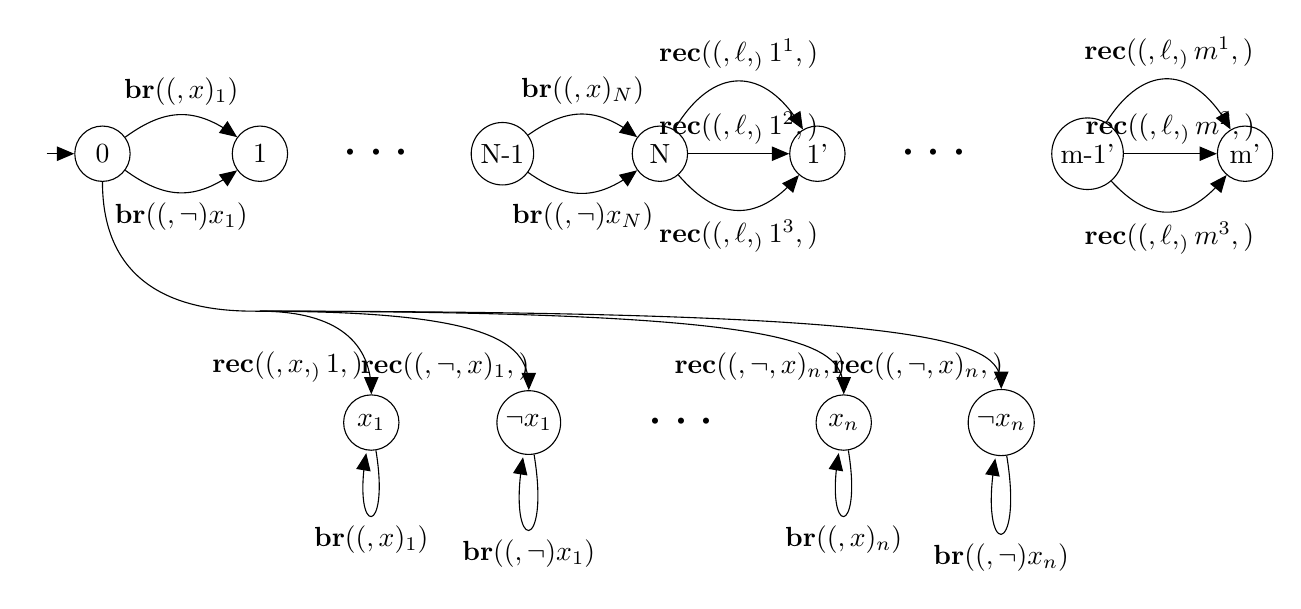
\begin{tikzpicture}[xscale=0.5,AUT style,node distance=2cm,auto,>= triangle
	45]
	\tikzstyle{initial}= [initial by arrow,initial text=,initial
	distance=.7cm]
	%	\tikzstyle{accepting}= [accepting by arrow,accepting text=,accepting
	%	distance=.7cm,accepting where =right]
	
	\node[state,initial, minimum width=0.1pt] (0) at (0,0) {0};
	
	\node[state] [right of=0] (1) {1};
	
	\node [right of=1, xshift=-20pt] (token1) {};
	\node [right of=token1, xshift=-50pt] (dots) {\huge $\cdots$};
	\node [right of=dots, xshift=-50pt] (token2) {};
	
	
	\node[state] [right of=token2, xshift=-20pt] (N-1) {N-1};
	\node[state] [right of=N-1] (N) {N};
	
	\node[state] [right of=N] (1') {1'};
	
	\node [right of=1', xshift=-20pt] (token3) {};
	\node [right of=token3, xshift=-50pt] (dots2) {\huge $\cdots$};
	\node [right of=dots2, xshift=-20pt] (token4) {};
	
	
	\node[state] [right of=token4, xshift=-40pt] (m-1) {m-1'};
	\node[state] [right of=m-1] (m) {m'};
	
	\coordinate[below of=1] (stop);
	\node[state] [below right of=stop] (r1) {$x_1$};
	\node [above left of=r1, yshift=-20pt, xshift=10pt] (r1') {$\rec(x_1, \enreg)$};
	\node[state] [right of=r1] (r1b) {$\neg x_1$};
	\node [above left of=r1b, yshift=-20pt, xshift=10pt] (r1b') {$\rec(\neg x_1, \enreg)$};
	\node [right of= r1b] (dots3) {\huge $\cdots$};
	\node[state] [right of=dots3] (rn) {$x_n$};
	\node [above left of=rn, yshift=-20pt, xshift=10pt] (rn') {$\rec(\neg x_n, \enreg)$};
	\node[state] [right of=rn] (rnb) {$\neg x_n$};
	\node [above left of=rnb, yshift=-20pt, xshift=10pt] (rnb') {$\rec(\neg x_n, \enreg)$};
	
	\draw (0) .. controls +(0,-2) and +(-1,0) .. (stop);
	\draw[->] (stop) .. controls +(2,0) and +(0,1) .. (r1);
	\draw[->] (stop) .. controls +(6,0) and +(0,1) .. (r1b);
	\draw[->] (stop) .. controls +(14,0) and +(0,1) .. (rn);
	\draw[->] (stop) .. controls +(18,0) and +(0,1) .. (rnb);
	\path[->, bend left=20]
	(0) edge node[above] {$\br(x_1)$} (1)
	(N-1) edge node[above] {$\br(x_N)$} (N) 	
	;
	\path[->, bend left=40]
	(N) edge node[above] {$\rec(\ell_1^1, \testeq)$} (1')
	(m-1) edge node[above] {$\rec(\ell_m^1, \testeq)$} (m) 	
	;
	\path[->, bend right=20] 
	(0) edge node[below] {$\br(\neg x_1)$} (1)
	(N-1) edge node[below] {$\br(\neg x_N)$} (N) 
	;
	\path[->, bend right=30] 
	(N) edge node[below] {$\rec(\ell_1^3, \testeq)$} (1')
	(m-1) edge node[below] {$\rec(\ell_m^3, \testeq)$} (m)	
	;
	\path[->]
	(N) edge node[above] {$\rec(\ell_1^2, \testeq)$} (1')
	(m-1) edge node[above] {$\rec(\ell_m^2, \testeq)$} (m) 	
	;
	\path[->, loop below]
	(r1) edge node[below] {$\br(x_1)$} (r1)
	(r1b) edge node[below] {$\br(\neg x_1)$} (r1b) 	
	(rn) edge node[below] {$\br(x_n)$} (rn)
	(rnb) edge node[below] {$\br(\neg x_n)$} (rnb) 	
	;
\end{tikzpicture}
	\caption{The "protocol" used for the NP-hardness proof.}
	\label{fig:np-hard}
\end{figure}

%We present here a reduction of the 3SAT problem to our problem.
Let $x_1, \ldots, x_n$ be variables and $\query = \bigwedge_{j=1}^m C_j$ with, for all $j$, $C_j = \ell_j^1 \lor \ell_j^2 \lor \ell_j^3$ and $\ell_j^1, \ell_j^2, \ell_j^3 \in \set{x_i, \neg x_i \mid 1 \leq i \leq n}$. 

Consider the "protocol" displayed in Figure~\ref{fig:np-hard}.
Our alphabet of messages is the set of literals $\set{x_i, \neg x_i \mid 1 \leq i \leq n}$.
Each agent may either receive a message, and repeat it forever or it may broadcast one of $x_i, \neg x_i$ for each $i$ and then try to receive a message one of $\ell_j^1, \ell_j^2, \ell_j^3$ for each $j$, with its own register value.

Suppose $\query$ is satisfiable, let $\nu$ be a satisfying assignment, then we set $\agents = \set{a, a_1, \ldots, a_n}$ as our set of agents. First for each $i$ we make $a$ broadcast $x_i$ if $\nu(x_i)= \top$ and $\neg x_i$ otherwise, this broadcast shall be received only by agent $a_i$. Agent $a_i$ will store $a$'s register value.
Then for each $j$ we select some $\ell_j^p$ satisfied by $\nu$. There exists $i$ such that $a_i$ is in state $\ell_j^p$. It broadcasts $\ell_j^p$ along with the initial register value of $a$, allowing $a$ to go to the next state.

As a result, there is an execution in which agent $a$ reaches $m'$.

Now suppose there is an execution $\run$ over some set of agents $\agents$ such that some agent $a \in \agents$ is in state $m'$ in the final configuration.
For each $i$, $a$ has broadcast either $x_i$ or $\neg x_i$, but not both.
Let $\nu$ be the valuation assigning $\top$ to $x_i$ if and only if $a$ has broadcast it.
The register of $a$ cannot have changed its value throughout the run. 
For each $j$ it has received one of $\ell_j^1, \ell_j^2, \ell_j^3$ along with its own initial register value (which we call $r$). Let $p_j$ be such that $a$ has received $\ell_j^{p_j}$.
Hence for all $j$ there exists an agent $a_j \in \agents$ such that at some point in the run the register value of $a_j$ is $r$ and $a_j$ broadcasts $\ell_j^{p_j}$.
This agent $a_j$ must be in state $\ell_j^{p_j}$ after receiving the broadcast $\brone{\ell_j^{p_j}}$ from $a$ (as all agents start with different register values).
Hence $\ell_j^{p_j}$ is satisfied by $\nu$. 

As a result, $\nu$ satisfies a literal of each clause of $\query$, and thus satisfies $\query$. This concludes our reduction.

%\end{proof}
%\fi

\begin{proposition}
	\label{prop:np-hard-query-cover}
	The "cover problem" is NP-hard.
\end{proposition}

\thmNPComplete*

\begin{proof}
	The lower bound is given by Proposition~\ref{prop:np-hard-query-cover}.
	For the upper bound, say we are given a "protocol" $\prot = (Q, \messages, \Delta, q_0, \regnum)$ and a state $q_f$. We have to verify that there exists a reachable configuration $\config_f$ convering $q_f$. By Proposition~\ref{prop:sound-and-complete}, it is the case if and only if there is an "abstract run" to an "abstract configuration" $(S,b, K)$ with $q_f \in S$.
	Furthermore, by Lemma~\ref{lem:short-run} if there is such an "abstract run" then there is one with at most $(\size{Q}+2)^3$ steps. 
	Thus we can simply guess such an abstract run and verify it in polynomial time.
	As a result, the "cover problem" is in \NP. 
\end{proof}
\end{document}